% !TEX program = tectonic
% Slides V2 « La couche données » — construit d'après PLAN_SLIDES_DONNEES.tex
% (une idée par slide, plan annoncé, chronologie, chiffres légendés, choix explicites, public neuf).
% RESTRUCTURATION 2026-07-17 (demande d'Alice) : « Donnée brute » et « Pipeline » FUSIONNÉES
% en PARTIE I — vision globale d'abord (0), puis 8 étapes numérotées, Chambre et Sénat
% traités ensemble à chaque étape (côte à côte quand ils diffèrent).
% FUSION 2026-07-17 (demande d'Alice) : Acquisition et Tri ne font plus qu'UNE étape (1),
% et l'on suit la Chambre EN ENTIER (1a acquisition → 1b tri type → 1c tri format)
% avant le Sénat (1d tri type → 1e tri format ; acquisition Sénat retirée = accès CSRF
% sans intérêt, le lien eFD suffit sur 1d) — l'alternance précédente « coupait la
% réflexion ». Tout l'aval a décalé
% d'un cran (ex-3 Extraction → 2 … ex-9 Table → 8) : 9 étapes → 8.
% Vérification = étape 9 de Partie I : Quiver + autres preuves. (univers retiré ; autres types & cohérence → Partie III)
% Périmètre : les DONNÉES seulement. Backtest et tables : hors périmètre.
% L'ancien deck SLIDES_DONNEES_S1S2.tex n'est PAS modifié.
% Chiffres : RAPPORT_QUALITE.md (source de vérité) + ANALYSE_FILING_TYPES_HOUSE.md
% + lignée v1-house (01_autres_filing_types/cache/) pour la Cohérence. Figures : png/{figs_deck,quality,figs_pop}/.
\documentclass[11pt,aspectratio=169]{beamer}
\definecolor{helec}{HTML}{3B6EA5}   % couleur maîtresse (Chambre électronique)
\usetheme{Madrid}
\usecolortheme[named=helec]{structure}
\setbeamertemplate{navigation symbols}{}
\setbeamertemplate{blocks}[rounded][shadow=false]
\setbeamerfont{frametitle}{series=\bfseries}
\usepackage[T1]{fontenc}
\usepackage{lmodern}
\usepackage[utf8]{inputenc}
\usepackage[french]{babel}
\usepackage{booktabs}
\usepackage{xcolor}
\usepackage{graphicx}
\usepackage{amssymb}
\usepackage{amsmath}
\usepackage{array}
\usepackage{newunicodechar}
\usepackage{tikz}
\usetikzlibrary{arrows.meta,positioning,calc}
\hypersetup{colorlinks=true, urlcolor=helec, linkcolor=white}

% Caractères Unicode → commandes (fontes T1)
\newunicodechar{→}{\ensuremath{\rightarrow}}
\newunicodechar{—}{\textemdash}
\newunicodechar{–}{\textendash}
\newunicodechar{…}{\ldots}
\newunicodechar{·}{\textperiodcentered}
\newunicodechar{≈}{\ensuremath{\approx}}
\newunicodechar{×}{\ensuremath{\times}}
\newunicodechar{≤}{\ensuremath{\leq}}
\newunicodechar{≥}{\ensuremath{\geq}}
\newunicodechar{−}{\ensuremath{-}}
\newunicodechar{✓}{\checkmark}
\newunicodechar{↔}{\ensuremath{\leftrightarrow}}
\newunicodechar{œ}{\oe}
\newunicodechar{Œ}{\OE}
\newunicodechar{°}{\textdegree}
\newunicodechar{§}{\S}
\newunicodechar{«}{\og}
\newunicodechar{»}{\fg{}}

% Code couleur des 4 voies
\definecolor{helec}{HTML}{3B6EA5}   % Chambre électronique
\definecolor{hocr}{HTML}{A9C5E2}    % Chambre OCR
\definecolor{selec}{HTML}{8E44AD}   % Sénat électronique
\definecolor{socr}{HTML}{CFAEDE}    % Sénat OCR
\definecolor{okgreen}{HTML}{2E8B57}
\definecolor{alertred}{HTML}{C0392B}
\definecolor{warnorange}{HTML}{E67E22}
\definecolor{dataC}{RGB}{176,110,14}
\definecolor{grisC}{RGB}{90,90,90}

\newcommand{\co}[1]{\texttt{#1}}
\tikzset{
  step/.style={rectangle, rounded corners=2pt, draw=#1, line width=0.8pt, fill=#1!8,
               align=center, font=\scriptsize, minimum height=0.72cm},
  bande/.style={rectangle, rounded corners=2pt, draw=#1, line width=0.8pt, fill=#1!8,
                align=center, font=\scriptsize, minimum height=0.62cm},
  arr/.style={-{Latex[length=2mm]}, line width=0.8pt, draw=gray!65},
}

% Tuile chiffre-clé : \tuile{couleur}{gros chiffre}{légende}
\newcommand{\tuile}[3]{%
  \begin{minipage}[t]{0.23\textwidth}\centering
    \colorbox{#1}{\parbox[c][21mm][c]{\dimexpr\linewidth-8pt}{\centering
      {\color{white}\Large\textbf{#2}}\\[0.6mm]
      {\color{white}\footnotesize #3}}}
  \end{minipage}}

\newcommand{\badge}[2]{\colorbox{#1}{\textcolor{white}{\footnotesize\textbf{#2}}}}
\newcommand{\badgel}[2]{\colorbox{#1}{\textcolor{black!80}{\footnotesize\textbf{#2}}}}

% Carte source : \carte{couleur}{titre}{contenu}
\newcommand{\carte}[3]{%
  \colorbox{#1!10}{\parbox[t][23mm][t]{\dimexpr\linewidth-8pt}{\vspace{1mm}
    {\color{#1}\footnotesize\textbf{#2}}\\[0.8mm]{\scriptsize #3}}}}

% Encadré CHOIX (un choix méthodologique, énoncé en une phrase)
\newcommand{\choixbox}[1]{%
  \colorbox{alertred!8}{\parbox{\dimexpr\linewidth-8pt}{\scriptsize
    \textbf{\textcolor{alertred}{CHOIX}}\; --- #1}}}

% Bandeau RÉPONSE (dernière slide d'une partie)
\newcommand{\repband}[1]{%
  \colorbox{okgreen!12}{\parbox{\dimexpr\textwidth-10pt}{\scriptsize
    \textbf{\textcolor{okgreen}{Réponse}}\; --- #1}}}

% Étiquette Chambre / Sénat (traitement côte à côte)
\newcommand{\chambre}{\textcolor{helec}{\textbf{Chambre}}}
\newcommand{\senat}{\textcolor{selec}{\textbf{Sénat}}}
% Bandeau « identique / différent » entre les deux chambres
\newcommand{\idem}[1]{\colorbox{grisC!10}{\parbox{\dimexpr\linewidth-8pt}{\scriptsize
  \textbf{\textcolor{grisC}{Chambre = Sénat}}\; --- #1}}}
\newcommand{\diff}[1]{\colorbox{warnorange!10}{\parbox{\dimexpr\linewidth-8pt}{\scriptsize
  \textbf{\textcolor{warnorange}{Chambre $\neq$ Sénat}}\; --- #1}}}

% ── Macros importées de la V1 (Parties Backtest & « autres ») ──
% Bande maths : \bmaths{noms de colonnes}{formule 1 ligne}
\newcommand{\bmaths}[2]{%
  {\scriptsize\color{black!55}#1}\\[0.2mm]
  {\small$\displaystyle #2$}\\[2mm]}
% Séparateur de partie plein cadre : \partdivider{couleur}{PARTIE X}{Grand titre}{sous-titre}
\newcommand{\partdivider}[4]{%
  {\setbeamercolor{background canvas}{bg=#1}
  \begin{frame}[plain]
    \centering\vfill
    {\color{white}\Large\textbf{#2}}\\[3.5mm]
    {\color{white!75}\rule{0.40\textwidth}{1pt}}\\[4.5mm]
    {\color{white}\fontsize{32}{36}\selectfont\textbf{#3}}\\[5.5mm]
    {\color{white!88}\large #4}
    \vfill
  \end{frame}}}
% Intercalaire de chapitre : \chapdivider{label}{Grand titre}{sous-titre}
\newcommand{\chapdivider}[3]{%
  \begin{frame}[plain]
    \centering\vfill
    {\color{helec!85}\large\textbf{#1}}\\[3.5mm]
    {\color{black!88}\fontsize{29}{33}\selectfont\textbf{#2}}\\[4mm]
    {\color{helec!45}\rule{0.30\textwidth}{1.2pt}}\\[4mm]
    {\color{black!55}\large #3}
    \vfill
  \end{frame}}

% Ligne d'étape dans un sommaire de partie : \etape{n}{titre}{glose}
\newcommand{\etape}[3]{%
  {\color{helec}\bfseries #1}\; & \textbf{#2} & {\scriptsize\color{black!60} #3}\\[0.6mm]}

% ── LE PIPELINE, dessin unique réutilisé ──
% \pipefig{k} : k = 0 → tout allumé (vue d'ensemble) ; k = 1..8 → seule l'étape k est
% allumée, le reste est estompé (repère « vous êtes ici »). Même dessin à chaque fois :
% seul le curseur bouge. La Partie I compte 8 étapes + la vérification (9).
% ⚠ Les lettres \opA..\opJ nomment les BANDES du dessin, PAS les étapes — depuis la
% fusion Acquisition+Tri (2026-07-17), l'étape 1 en allume deux. Correspondance :
%   étape 1 = \opA acquisition + \opB tri        étape 5 = \opF secteur  + \opJ
%   étape 2 = \opC extraction                    étape 6 = \opG dédup    + \opJ
%   étape 3 = \opD identité                      étape 7 = \opH entonnoir (+ prix)
%   étape 4 = \opE ticker                        étape 8 = \opI table de recherche
%   \opJ = la TABLE DU CORPUS (la frontière de sortie du pipeline), allumée en 5 et 6.
\newcommand{\pipefig}[1]{%
  \def\opA{0.16}\def\opB{0.16}\def\opC{0.16}\def\opD{0.16}\def\opE{0.16}%
  \def\opF{0.16}\def\opG{0.16}\def\opH{0.16}\def\opI{0.16}\def\opJ{0.16}\def\opK{0.16}%
  \ifnum#1=0 \def\opA{1}\def\opB{1}\def\opC{1}\def\opD{1}\def\opE{1}%
             \def\opF{1}\def\opG{1}\def\opH{1}\def\opI{1}\def\opJ{1}\def\opK{1}\fi
  \ifnum#1=1 \def\opA{1}\def\opB{1}\fi
  \ifnum#1=2 \def\opC{1}\fi  \ifnum#1=3 \def\opD{1}\fi  \ifnum#1=4 \def\opE{1}\fi
  \ifnum#1=5 \def\opF{1}\def\opJ{1}\fi
  \ifnum#1=6 \def\opG{1}\def\opJ{1}\fi
  \ifnum#1=7 \def\opH{1}\fi  \ifnum#1=8 \def\opI{1}\fi
  \ifnum#1=9 \def\opK{1}\fi
  \begin{tikzpicture}[node distance=3mm, every node/.style={transform shape}]
    % ---------- 1 · Acquisition ----------
    \begin{scope}[opacity=\opA, text opacity=\opA]
      \node[step=helec, text width=5.6cm] (acqH) at (-3.6,0)
        {\textbf{\color{helec}Chambre} --- \emph{House Clerk} : index → PDF
         \;·\; \textbf{8\,252 PTR}};
      \node[step=selec, text width=5.6cm] (acqS) at (3.6,0)
        {\textbf{\color{selec}Sénat} --- \emph{eFD} : recherche → liste
         \;·\; \textbf{2\,153 PTR}};
      % une seule étiquette pour l'étape 1 : elle couvre l'acquisition ET le tri,
      % d'où sa position entre les deux rangées.
      \node[font=\tiny\bfseries, text=helec!80, align=left] at (-7.9,-0.62)
        {1 Acquisition\\\& Tri};
    \end{scope}
    % ---------- 1 · Tri (même étape que l'acquisition : \opA et \opB s'allument ensemble)
    \begin{scope}[opacity=\opB, text opacity=\opB]
      \node[step=helec, text width=2.6cm] (hpdf) at (-5.3,-1.4)
        {\textbf{PDF lisible}\\texte\\[0.2mm]{\scriptsize\color{helec}\textbf{5\,828 PTR}}};
      \node[step=hocr, text width=2.6cm] (hscan) at (-1.9,-1.4)
        {\textbf{PDF scanné}\\image\\[0.2mm]{\scriptsize\color{black!80}\textbf{2\,424 PTR}}};
      \node[step=selec, text width=2.6cm] (shtml) at (1.9,-1.4)
        {\textbf{page web}\\texte\\[0.2mm]{\scriptsize\color{selec}\textbf{1\,780 PTR}}};
      \node[step=socr, text width=2.6cm] (sgif) at (5.3,-1.4)
        {\textbf{papier scanné}\\image\\[0.2mm]{\scriptsize\color{black!80}\textbf{373 PTR}}};
      \node[step=alertred, text width=2.6cm, font=\tiny] (hC) at (-1.9,-2.55)
        {\textbf{manuscrit} → écarté \;\textbf{−582}};
      % marqueur de niveau (marge droite) : au tri, on compte des DOCUMENTS
      \node[align=center, font=\scriptsize\bfseries, text=helec!85, text width=2.4cm]
        (mDoc) at (7.9,-1.4) {\rule{2.2cm}{0.6pt}\\[0.4mm]DOCUMENTS\\{\tiny (PTR déposés)}};
    \end{scope}
    % ---------- 2 · Extraction ---------- (chiffres BRUTS, avant dédup : leur somme = 170 920)
    \begin{scope}[opacity=\opC, text opacity=\opC]
      \node[step=helec, text width=2.6cm] (hpar) at (-5.3,-2.9)
        {\textbf{parsing}\\[0.3mm]{\small\textbf{\color{helec}58\,756}}\,{\tiny txns}};
      \node[step=hocr, text width=2.6cm] (hvis) at (-1.9,-3.6)
        {\textbf{OCR Vision}\\[0.3mm]{\small\textbf{\color{helec}93\,325}}\,{\tiny txns}};
      \node[step=selec, text width=2.6cm] (spar) at (1.9,-2.9)
        {\textbf{tableaux}\\[0.3mm]{\small\textbf{\color{selec}14\,813}}\,{\tiny txns}};
      \node[step=socr, text width=2.6cm] (svis) at (5.3,-2.9)
        {\textbf{OCR Vision}\\[0.3mm]{\small\textbf{\color{selec}4\,026}}\,{\tiny txns}};
      \node[font=\tiny, text=black!55, align=center, text width=9.6cm] at (-1.9,-4.35)
        {chaque \textbf{transaction} extraite porte ses \textbf{7 champs} ---
         \emph{qui · quand · quoi · sens · fourchette · détenteur · chambre} ---
         et son \textbf{montant} (milieu de la fourchette)};
      \node[font=\tiny\bfseries, text=helec!80] at (-7.9,-3.1) {2 Extraction};
      % marqueur de niveau (marge droite) : à l'extraction, on compte des TRANSACTIONS
      \node[align=center, font=\scriptsize\bfseries, text=dataC, text width=2.6cm]
        (mTxn) at (7.9,-3.15) {\rule{2.3cm}{0.6pt}\\[0.4mm]TRANSACTIONS\\{\tiny 1 PTR $\to$ plusieurs}};
    \end{scope}
    % ---------- 3 à 6 · le tronc commun ----------
    \begin{scope}[opacity=\opD, text opacity=\opD]
      \node[bande=grisC, text width=12.6cm] (ident) at (0,-4.95)
        {\textbf{identité} --- nom libre → identifiant officiel de l'élu \;·\; \textbf{100\,\%}};
      \node[font=\tiny\bfseries, text=helec!80] at (-7.9,-4.95) {3 Identité};
    \end{scope}
    \begin{scope}[opacity=\opE, text opacity=\opE]
      \node[bande=dataC, text width=12.6cm] (tick) at (0,-5.75)
        {\textbf{ticker} --- sur \textbf{tous les actifs} : \textbf{84,1\,\%} des transactions
         ont un symbole (Ch.)\ · \textbf{77,9\,\%} (Sén.) --- le reste = \textbf{surtout du non coté}};
      \node[font=\tiny\bfseries, text=helec!80] at (-7.9,-5.75) {4 Ticker};
    \end{scope}
    \begin{scope}[opacity=\opF, text opacity=\opF]
      \node[bande=dataC, text width=12.6cm] (sect) at (0,-6.55)
        {\textbf{secteur} --- GICS → ETF \;·\; sur \textbf{toutes les transactions} :
         \textbf{79,8\,\%} ont un secteur (Ch.)\ · \textbf{70,4\,\%} (Sén.)};
      \node[font=\tiny\bfseries, text=helec!80] at (-7.9,-6.55) {5 Secteur};
    \end{scope}
    % ---------- la sortie du pipeline (frontière) ----------
    \begin{scope}[opacity=\opJ, text opacity=\opJ]
      \node[bande=dataC, fill=dataC!16, text width=12.6cm] (corp) at (0,-7.35)
        {\textbf{TABLE DU CORPUS} --- \textbf{170\,920 lignes × 28 colonnes}};
    \end{scope}
    \begin{scope}[opacity=\opG, text opacity=\opG]
      \node[bande=grisC, text width=12.6cm] (ded) at (0,-8.2)
        {\textbf{dédoublonnage} --- un même trade re-déclaré compté \textbf{une seule fois},
         par l'empreinte à 7 champs : \textbf{−1\,920}
         re-divulgations → \textbf{169\,000 transactions uniques}};
      \node[font=\tiny\bfseries, text=helec!80] at (-7.9,-8.2) {6 Dédup};
    \end{scope}
    % ---------- 7 · Entonnoir : deux filtres consécutifs, lignes puis symboles ----------
    \begin{scope}[opacity=\opH, text opacity=\opH]
      \node[bande=okgreen, text width=12.6cm] (ent) at (0,-9.05)
        {\textbf{entonnoir des LIGNES} --- on ne garde que ce qu'un backtest peut valoriser :
         \textbf{action ou ETF coté}, date, sens et montant valides → \textbf{−34\,536}
         (surtout du non-coté : obligations, fonds)};
      \node[font=\tiny\bfseries, text=helec!80] at (-7.9,-9.05) {7 Entonnoir};
      \node[bande=okgreen, text width=12.6cm] (sym) at (0,-9.85)
        {\textbf{entonnoir des SYMBOLES} --- a-t-on un \textbf{vrai cours de bourse} ?
         4\,618 symboles → \textbf{3\,289} avec un historique de prix propre →
         \textbf{118\,029} trades valorisables (≈\,88\,\%)};
      \node[font=\tiny\bfseries, text=helec!80] at (-7.9,-9.85) {· prix};
    \end{scope}
    % ---------- 8 · Table finale (LE LIVRABLE) ----------
    \begin{scope}[opacity=\opI, text opacity=\opI]
      \node[bande=okgreen, fill=okgreen!16, text width=12.6cm] (fin) at (0,-10.75)
        {\textbf{TABLE DE RECHERCHE} --- ces \textbf{118\,029} trades, 36 colonnes
         \;{\tiny(le livrable, après les 2 entonnoirs)}};
      \node[font=\tiny\bfseries, text=helec!80] at (-7.9,-10.75) {8 Table};
    \end{scope}
    % ---------- 9 · Vérifier (après la table : peut-on lui faire confiance ?) ----------
    \begin{scope}[opacity=\opK, text opacity=\opK]
      \node[bande=helec, fill=helec!16, text width=12.6cm] (verif) at (0,-11.6)
        {\textbf{VÉRIFIER} --- la table est-elle \textbf{fiable} ? corroboration \textbf{Quiver}
         + autres preuves indépendantes};
      \node[font=\tiny\bfseries, text=helec!80] at (-7.9,-11.6) {9 Vérifier};
    \end{scope}
    % ---------- les flèches ----------
    \begin{scope}[opacity=0.30]
      \draw[arr] (acqH) -- (hpdf); \draw[arr] (acqH) -- (hscan);
      \draw[arr] (acqS) -- (shtml); \draw[arr] (acqS) -- (sgif);
      \draw[arr] (hscan) -- (hC);
      \draw[arr] (hpdf) -- (hpar); \draw[arr] (hscan) -- (hvis);
      \draw[arr] (shtml) -- (spar); \draw[arr] (sgif) -- (svis);
      \draw[arr] (hpar.south) -- (ident.north -| hpar.south);
      \draw[arr] (hvis.south) -- (ident.north -| hvis.south);
      \draw[arr] (spar.south) -- (ident.north -| spar.south);
      \draw[arr] (svis.south) -- (ident.north -| svis.south);
      \draw[arr] (ident) -- (tick); \draw[arr] (tick) -- (sect);
      \draw[arr] (sect) -- (corp); \draw[arr] (corp) -- (ded);
      \draw[arr] (ded) -- (ent); \draw[arr] (ent) -- (sym); \draw[arr] (sym) -- (fin);
    \draw[arr] (fin) -- (verif);
    \end{scope}
  \end{tikzpicture}}

% Slide-repère « vous êtes ici » : \pipeslide{k}{titre}{question}{ce qu'on en sort}
\newcommand{\pipeslide}[4]{%
  \begin{frame}{#2}
    \centering
    \resizebox{!}{0.66\textheight}{\pipefig{#1}}\\[2mm]
    \colorbox{helec!10}{\parbox{0.92\textwidth}{\centering\footnotesize\vspace{0.5mm}
      \emph{#3}\\[0.8mm]{\scriptsize\color{black!65} ce qu'on en sort : #4}\vspace{0.5mm}}}
  \end{frame}}

% ── Images cliquables « agrandir » : pastille loupe en coin + zoom plein écran (frames en annexe) ──
% \clickzoom{label}{image} : rend l'image cliquable vers la frame `zoom-label`, pose l'ancre retour.
\newcommand{\clickzoom}[2]{%
  \hypertarget{back-#1}{}%
  \hyperlink{zoom-#1}{%
    \tikz[baseline=(zc.south)]{%
      \node[inner sep=0] (zc) {#2};
      \node[anchor=north east, fill=selec, text=white, font=\tiny\bfseries,
            inner sep=1.4pt, rounded corners=1.5pt]
            at ([shift={(-1.2pt,-1.2pt)}]zc.north east) {$\oplus$};}}}
% \zoomframe{label}{chemin} : image plein écran, cliquable pour revenir à la slide (back-label).
\newcommand{\zoomframe}[2]{%
  \begin{frame}[plain]
    \hypertarget{zoom-#1}{}%
    \centering
    \hyperlink{back-#1}{%
      \includegraphics[width=0.92\paperwidth,height=0.9\paperheight,keepaspectratio]{#2}}%
  \end{frame}}
% Pied de page = réplique Madrid, mais le total = dernière page de contenu (\label{endmain}),
% pour que les frames de zoom (agrandissements, après endmain) ne gonflent pas le compteur.
\setbeamertemplate{footline}{%
  \leavevmode%
  \hbox{%
  \begin{beamercolorbox}[wd=.333333\paperwidth,ht=2.25ex,dp=1ex,center]{author in head/foot}%
    \usebeamerfont{author in head/foot}\insertshortauthor~(\insertshortinstitute)%
  \end{beamercolorbox}%
  \begin{beamercolorbox}[wd=.333333\paperwidth,ht=2.25ex,dp=1ex,center]{title in head/foot}%
    \usebeamerfont{title in head/foot}\insertshorttitle%
  \end{beamercolorbox}%
  \begin{beamercolorbox}[wd=.333333\paperwidth,ht=2.25ex,dp=1ex,right]{title in head/foot}%
    \usebeamerfont{title in head/foot}\insertshortdate{}\hspace*{2em}%
    \insertframenumber{} / \pageref{endmain}\hspace*{2ex}%
  \end{beamercolorbox}}%
  \vskip0pt%
}

\title[La couche données]{La couche données --- collecte \& validation}
\subtitle{Transactions boursières du Congrès américain · Chambre \& Sénat · 2014--2026}
\author[A.~Lemaire]{Alice Lemaire}
\institute[Ramify]{Document de recherche --- livrable Ramify}
\date{Juillet 2026}


% ── macros importées du deck backtest (pour la Partie II fusionnée) ──
\newcommand{\kpi}[3]{{\large\textbf{\textcolor{#1}{#2}}}~{\footnotesize #3}}
\newcommand{\defl}[1]{{\scriptsize\color{black!55}#1}}
\newcommand{\barreau}[2]{%
  \colorbox{helec}{\textcolor{white}{\footnotesize\textbf{~Test #1~}}}\;{\footnotesize\textbf{#2}}}
\tikzset{rung/.style={rectangle, rounded corners=3pt, draw=helec, line width=1pt,
  fill=helec!8, align=center, font=\footnotesize, minimum height=1.05cm, text width=2.35cm}}

\begin{document}

% ── Titre ──
\begin{frame}[plain]
  \titlepage
\end{frame}

% ══════════════════ OUVERTURE ══════════════════

% ── O1 · Le pourquoi ──
\begin{frame}{Depuis 2012, chaque élu du Congrès doit déclarer ses transactions en bourse}
  \centering
  {\normalsize le \textbf{STOCK Act} (2012) : toute transaction boursière de plus de
   1\,000~\$ d'un élu doit être déclarée dans un\\
   \emph{Periodic Transaction Report} (« \textbf{PTR} »)}\\[5mm]
  \tuile{helec}{45 j}{le délai légal pour\\déclarer un trade}\hfill
  \tuile{grisC}{2014--2026}{la fenêtre étudiée\\(la loi date de 2012)}\hfill
  \tuile{dataC}{2 chambres}{435 représentants\\+ 100 sénateurs}\\[5mm]
  \colorbox{helec!10}{\parbox{0.86\textwidth}{\centering\footnotesize\vspace{0.8mm}
    \textbf{la question de recherche} : ces déclarations publiques peuvent-elles nourrir
    une stratégie d'investissement ?\vspace{0.8mm}}}
\end{frame}

% ── O3 · Le plan : deux parties ──
% ── Slide « Le plan --- deux parties » RETIRÉE (2026-07-19, demande Alice) : plan pas à jour,
%    beaucoup de changements à venir ; à refaire une fois la structure stabilisée. ──

% ══════════════════ PARTIE I ══════════════════
\section{Partie I · Construire la table}

\begin{frame}[plain]
  \centering
  \vspace{12mm}
  {\color{helec!85}\large\textbf{PARTIE I}}\\[3mm]
  {\color{black!88}\fontsize{30}{34}\selectfont\textbf{Construire la table}}\\[3mm]
  {\color{helec!45}\rule{0.30\textwidth}{1.2pt}}\\[3mm]
  {\color{black!55}\large De $\sim$10\,000 documents publics hétérogènes à une seule table}
  \vspace{4mm}
  {\footnotesize\color{black!50}{\color{selec}$\oplus$}~ toutes les images du deck sont
   \textbf{cliquables} pour être agrandies (re-cliquez pour revenir).}
  \vspace{8mm}
\end{frame}

% ── 0 · Le pipeline complet ──
\begin{frame}{0 · Le pipeline complet --- tout le trajet de la donnée}
  \centering
  \resizebox{!}{0.78\textheight}{\pipefig{0}}
\end{frame}

% ════ 1 · ACQUISITION & TRI ════
\pipeslide{1}{1 · Acquisition \& Tri}%
  {Où vivent ces déclarations, lesquelles faut-il lire --- et dans quel état
   arrivent-elles ?}%
  {l'univers à traiter --- \textbf{8\,252} PTR à la \chambre{}, que l'index officiel
   \emph{déclare} \;·\; \textbf{2\,153} au \senat{}, qu'il faut \emph{recenser} ---
   répartis en \textbf{4 sous-corpus} (chambre × format)}

% ── 1a · Acquisition Chambre ──
\begin{frame}{1a · Chambre · acquisition --- récupérer les dépôts depuis l'index annuel}
  \begin{columns}[T]
    \begin{column}{0.40\textwidth}\centering
      \fcolorbox{black!25}{white}{\clickzoom{site_house_clerk}{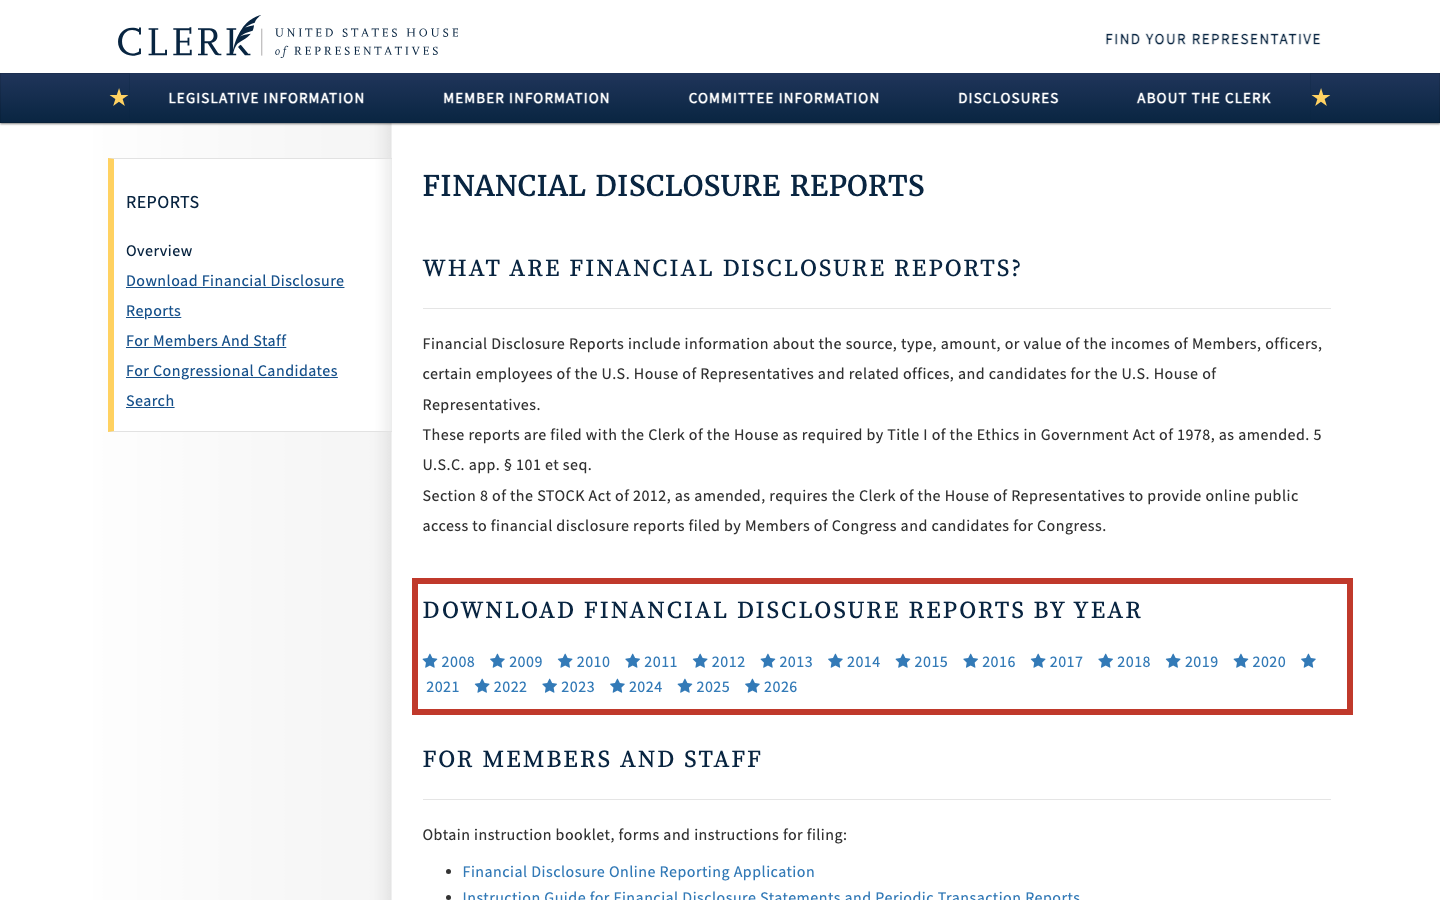
\includegraphics[width=0.95\linewidth,height=22mm,keepaspectratio]{png/figs_deck/site_house_clerk.png}}}\\[0.8mm]
      {\scriptsize \href{https://disclosures-clerk.house.gov/FinancialDisclosure}{\texttt{disclosures-clerk.house.gov}}}\\[1.5mm]
      \begin{tikzpicture}[node distance=1.6mm]
        \node[bande=helec, text width=4.6cm] (z) {une \textbf{archive par année}, 2014→2026};
        \node[bande=helec, text width=4.6cm, below=of z] (x) {elle contient l'\textbf{index annuel}};
        \node[bande=helec, text width=4.6cm, below=of x] (i) {un bloc par \textbf{dépôt}};
        \node[bande=okgreen, text width=4.6cm, below=of i] (u) {le \textbf{n\textsuperscript{o} (DocID)} donne l'\textbf{URL} du PDF};
        \draw[arr] (z) -- (x); \draw[arr] (x) -- (i); \draw[arr] (i) -- (u);
      \end{tikzpicture}
    \end{column}
    \begin{column}{0.57\textwidth}\centering
      \clickzoom{fichier_index_xml}{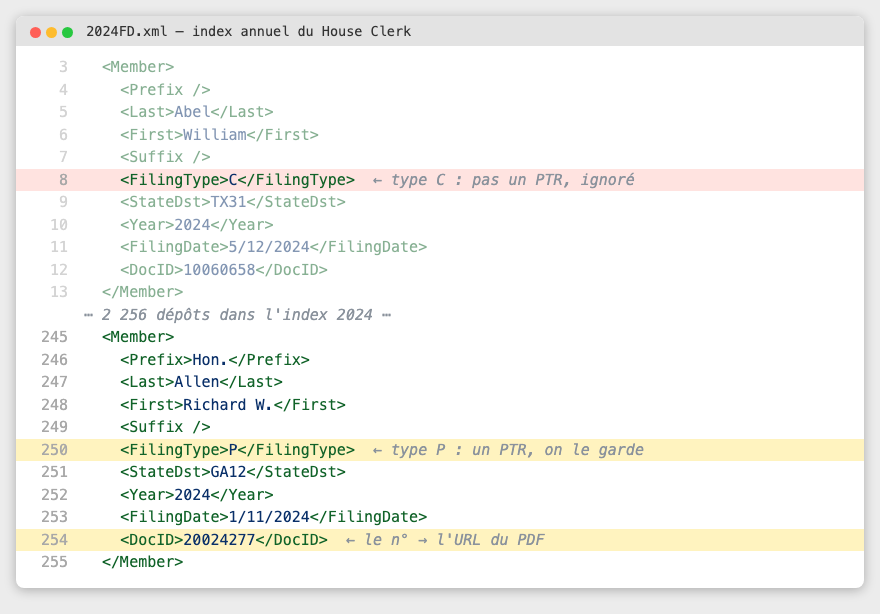
\includegraphics[width=0.94\linewidth,height=37mm,keepaspectratio]{png/figs_deck/fichier_index_xml.png}}\\[0.5mm]
      {\scriptsize\color{black!60} l'index réel : chaque dépôt y déclare son type, sa
       \textbf{date de dépôt (divulgation)} et son numéro de document}\\[1mm]
      {\scriptsize \textbf{exemple} --- le dépôt surligné (\textbf{n\textsuperscript{o} 20024277})
       s'ouvre à :\\
       \url{https://disclosures-clerk.house.gov/public_disc/ptr-pdfs/2024/20024277.pdf}}
    \end{column}
  \end{columns}
  \vspace{1mm}
  \centering
  {\footnotesize \textbf{35\,315} dépôts de tous types · \textbf{13 années} couvertes}
\end{frame}

% ── 1b · Tri Chambre ──
\begin{frame}{1a · Chambre · tri --- choisir les PTR : on lit la lettre \textbf{P} dans l'index}
  \centering
  \vspace{0.5mm}
  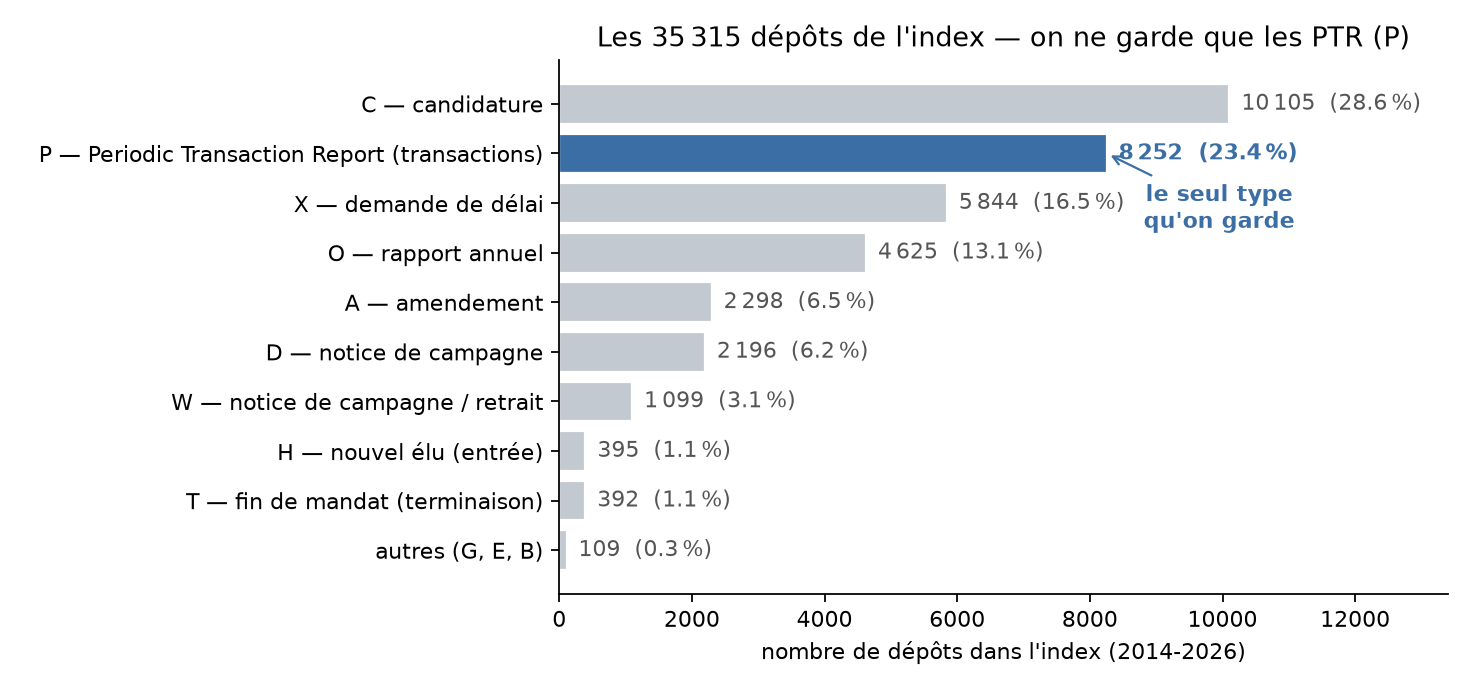
\includegraphics[width=0.70\textwidth,height=0.52\textheight,keepaspectratio]{png/figs_deck/fig_filingtypes.png}\\[3mm]
  {\footnotesize l'index déclare le \textbf{type} de chaque dépôt --- on ne garde que le
   type \textbf{P} (les \textbf{PTR}, les seules transactions datées) :
   \textbf{8\,252 sur 35\,315}}\\[1.5mm]
  {\footnotesize\color{black!60} les \textbf{11 autres types} pourraient être intéressants
   --- on les \textbf{regardera dans une autre partie}}
\end{frame}

% ── 1c · Tri Chambre · format (lisible vs scanné) ──
\begin{frame}{1a · Chambre · tri --- distinguer les PTR lisibles des scannés}
  \centering
  \vspace{1mm}
  {\footnotesize le \textbf{DocID} annonce déjà le format --- il commence par
   \textbf{\co{2\ldots}} = \textbf{lisible}, ou par \textbf{\co{8\ldots}}/\textbf{\co{9\ldots}}
   = \textbf{scanné} :}\\[3mm]
  \begin{columns}[T]
    \begin{column}{0.46\textwidth}\centering
      \fcolorbox{helec}{white}{\clickzoom{house_digital}{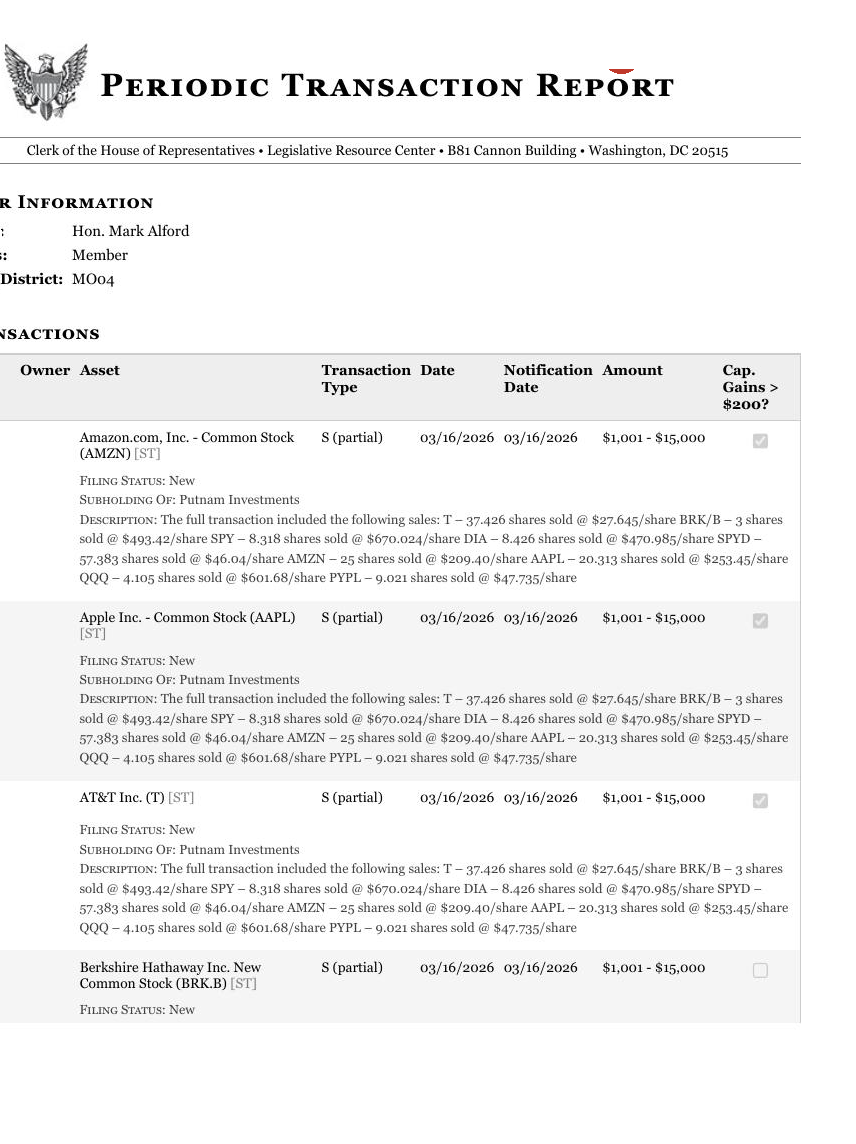
\includegraphics[width=0.58\linewidth,height=0.40\textheight,keepaspectratio]{png/figs_deck/house_digital.png}}}\\[1.2mm]
      \badge{helec}{PDF lisible --- 71\,\%}\\[0.6mm]
      {\scriptsize couche texte, lu directement \;·\; DocID en \co{2\ldots}}
    \end{column}
    \begin{column}{0.46\textwidth}\centering
      \fcolorbox{hocr}{white}{\clickzoom{house_ocr}{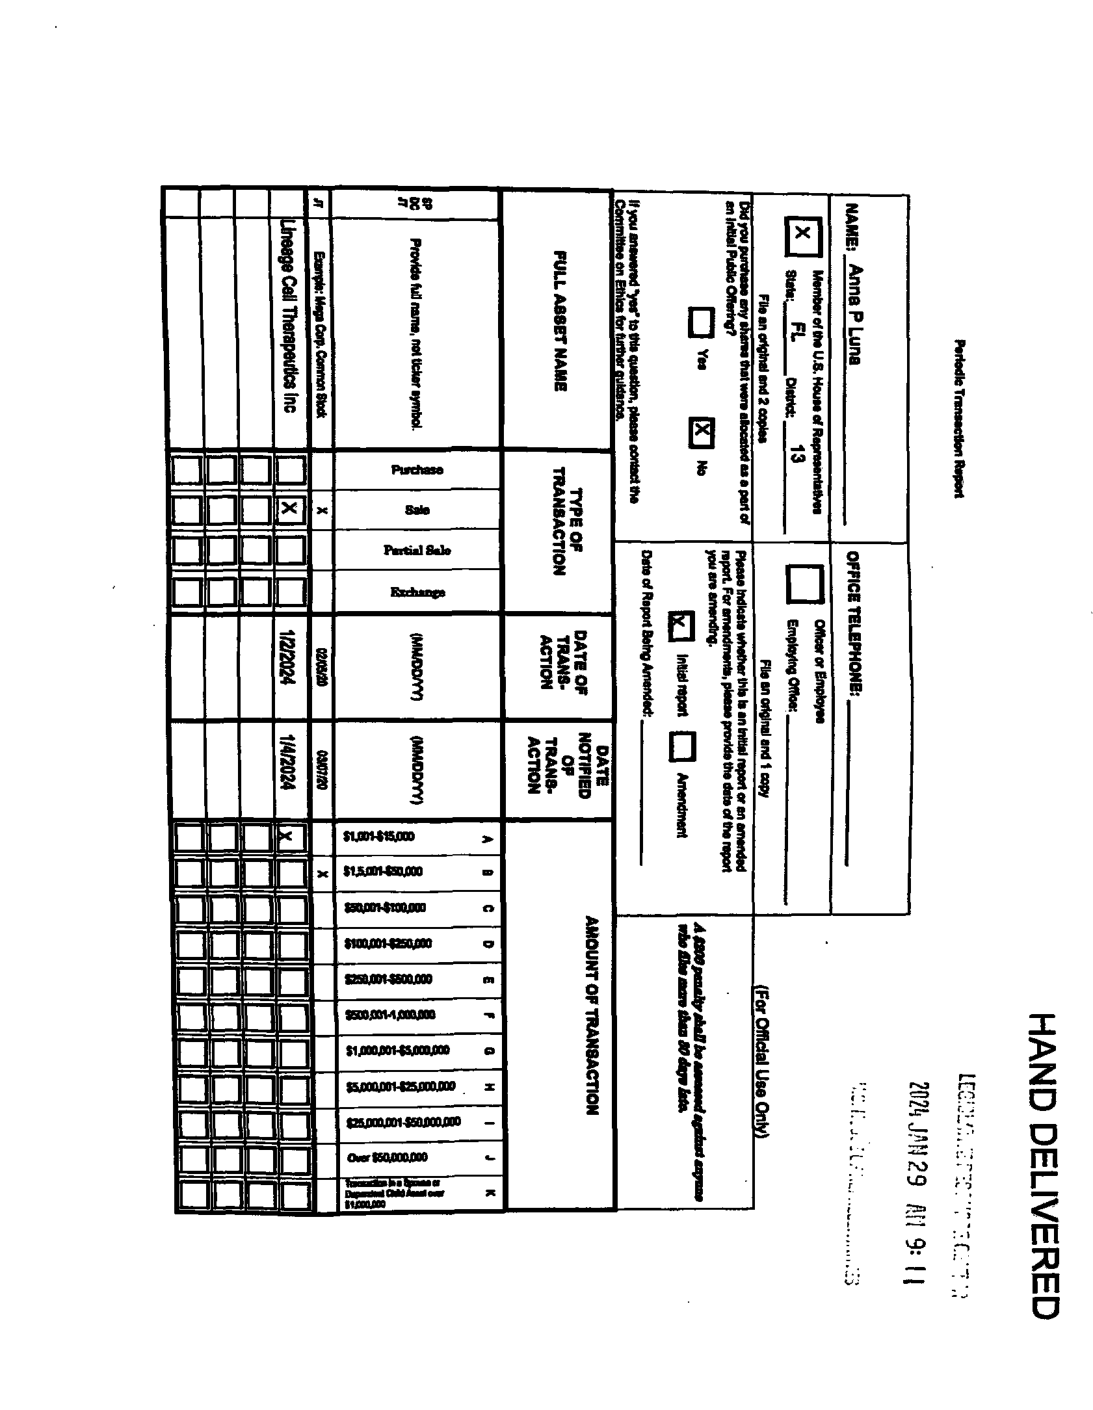
\includegraphics[width=0.58\linewidth,height=0.40\textheight,keepaspectratio]{png/figs_deck/house_ocr.png}}}\\[1.2mm]
      \badgel{hocr}{PDF scanné --- 29\,\%}\\[0.6mm]
      {\scriptsize image, à lire par \textbf{OCR} \;·\; DocID en \co{8\ldots}/\co{9\ldots}}
    \end{column}
  \end{columns}
\end{frame}

% ── 1d · Tri Sénat · type (PTR tous membres + liste + figure type & déposant) ──
\begin{frame}{1b · Sénat --- choisir les PTR de tous les membres}
  \begin{columns}[T]
    \begin{column}{0.40\textwidth}\centering
      \fcolorbox{black!25}{white}{\clickzoom{site_senate_form}{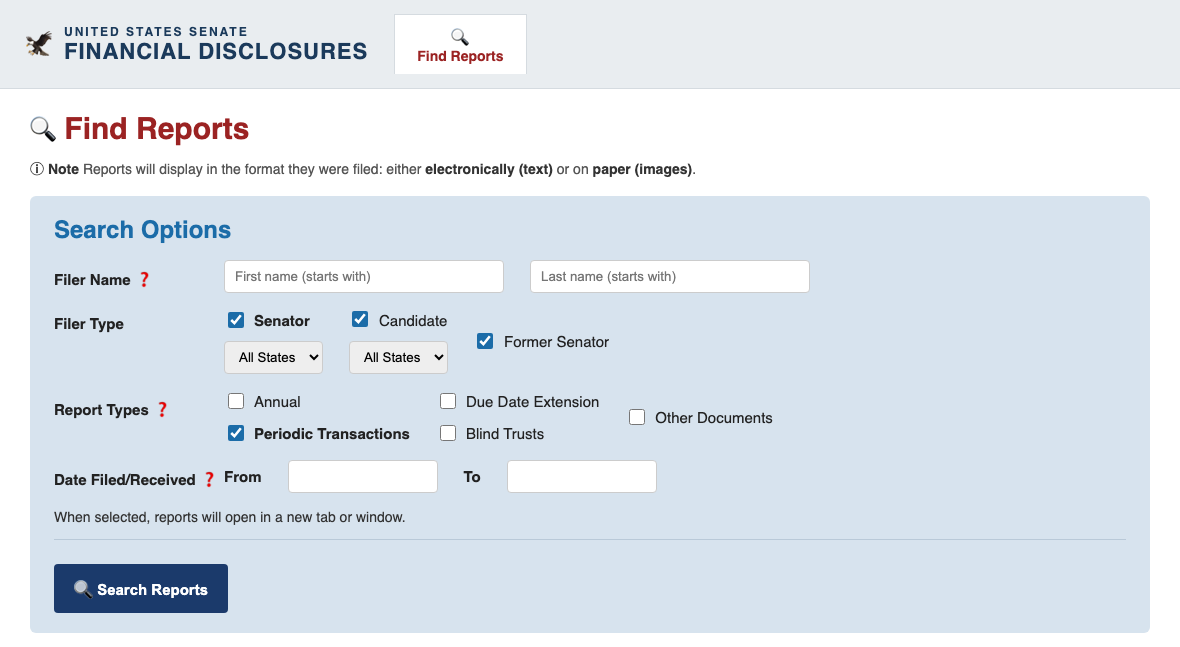
\includegraphics[width=\linewidth,height=0.42\textheight,keepaspectratio]{png/figs_deck/site_senate_form.png}}}\\[0.6mm]
      {\scriptsize \href{https://efdsearch.senate.gov/search/home/}{\texttt{efdsearch.senate.gov}}}\\[0.6mm]
      {\scriptsize\color{black!60} on coche \textbf{PTR} pour \textbf{tous les déposants} → la liste des dépôts}
    \end{column}
    \begin{column}{0.57\textwidth}\centering
      \badge{selec}{2\,160 \emph{Periodic Transactions} = \textbf{42\,\%} des \textbf{5\,096} dépôts}\\[1.2mm]
      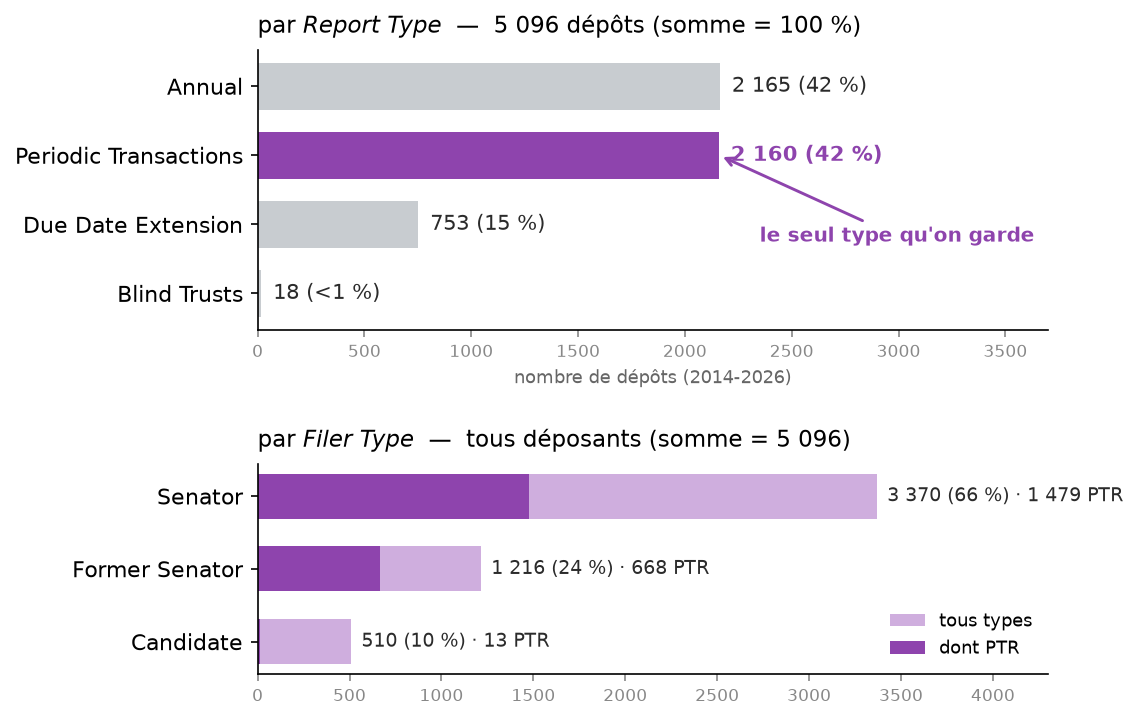
\includegraphics[width=\linewidth,height=0.62\textheight,keepaspectratio]{png/figs_deck/fig_senat_types.png}
    \end{column}
  \end{columns}
  \vspace{2mm}
  {\footnotesize on \textbf{choisit les PTR} --- les autres types \textbf{dans une autre partie}
   \;·\; {\color{black!55}les \textbf{13 PTR} de candidats sont tous d'un \textbf{sénateur réélu}
   (Sessions) ; \textbf{31\,\%} des PTR = anciens sénateurs}}
\end{frame}

% ── 1e · Tri Sénat · format (page web vs papier scanné) ──
\begin{frame}{1b · Sénat --- distinguer page web et papier scanné}
  \centering
  \vspace{1mm}
  {\footnotesize au \senat{}, chaque dépôt s'ouvre soit en \textbf{page web} (texte),
   soit en \textbf{image scannée} (à lire par OCR) :}\\[4mm]
  \begin{columns}[T]
    \begin{column}{0.46\textwidth}\centering
      \fcolorbox{selec}{white}{\clickzoom{senate_digital_1}{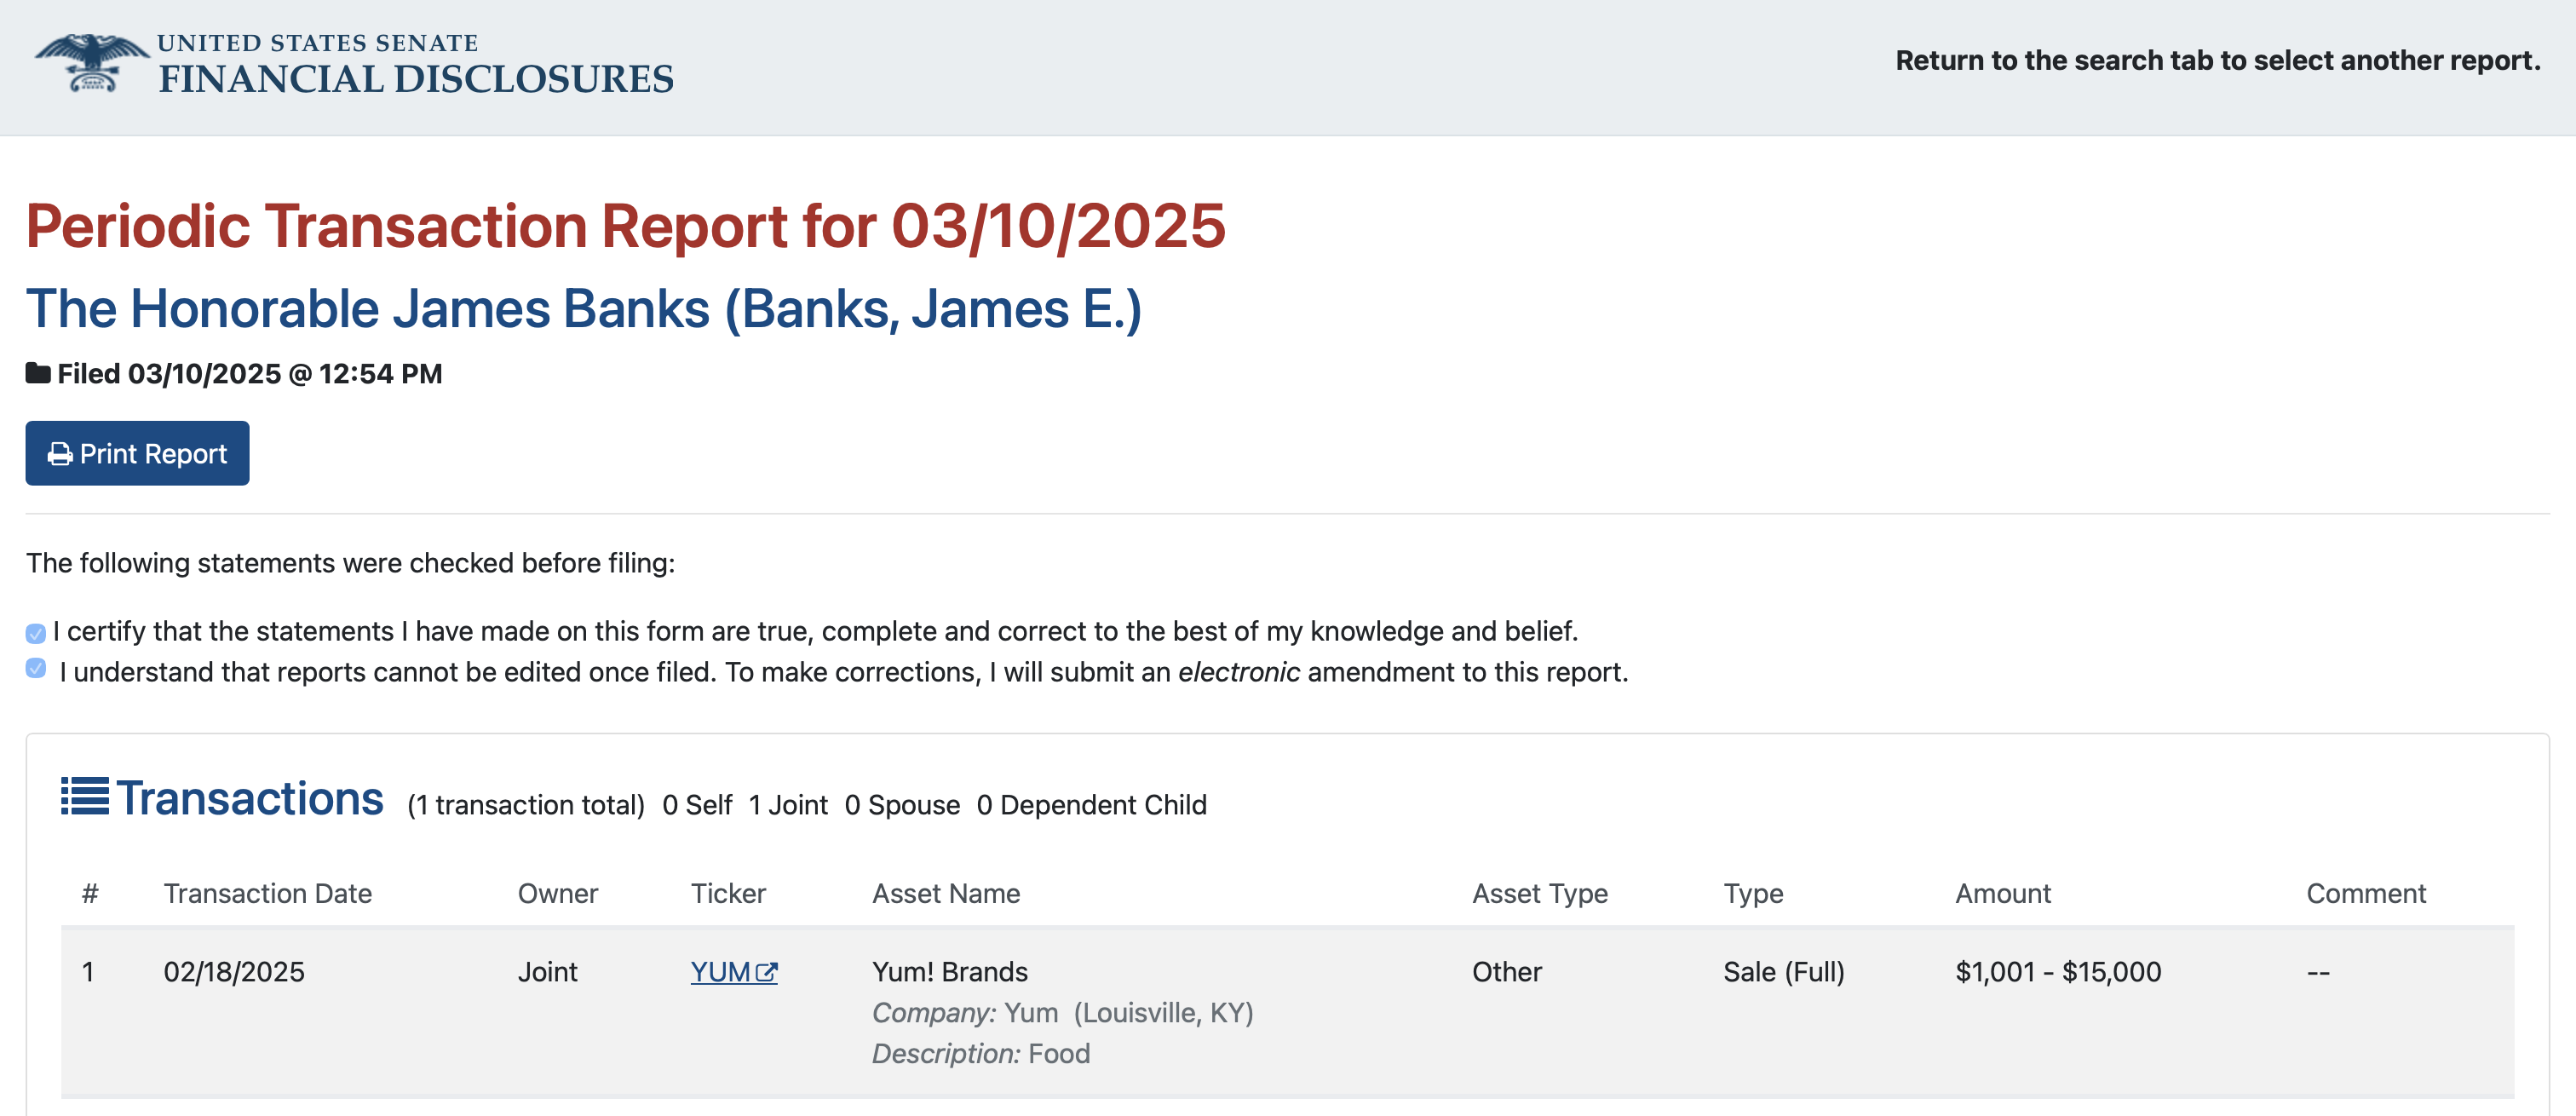
\includegraphics[width=0.72\linewidth,height=0.42\textheight,keepaspectratio]{png/figs_deck/senate_digital.png}}}\\[1.5mm]
      \badge{selec}{page web --- 1\,780}\\[0.8mm]
      {\scriptsize table déjà propre, lue directement}
    \end{column}
    \begin{column}{0.46\textwidth}\centering
      \fcolorbox{socr}{white}{\clickzoom{senat_papier_droit_1}{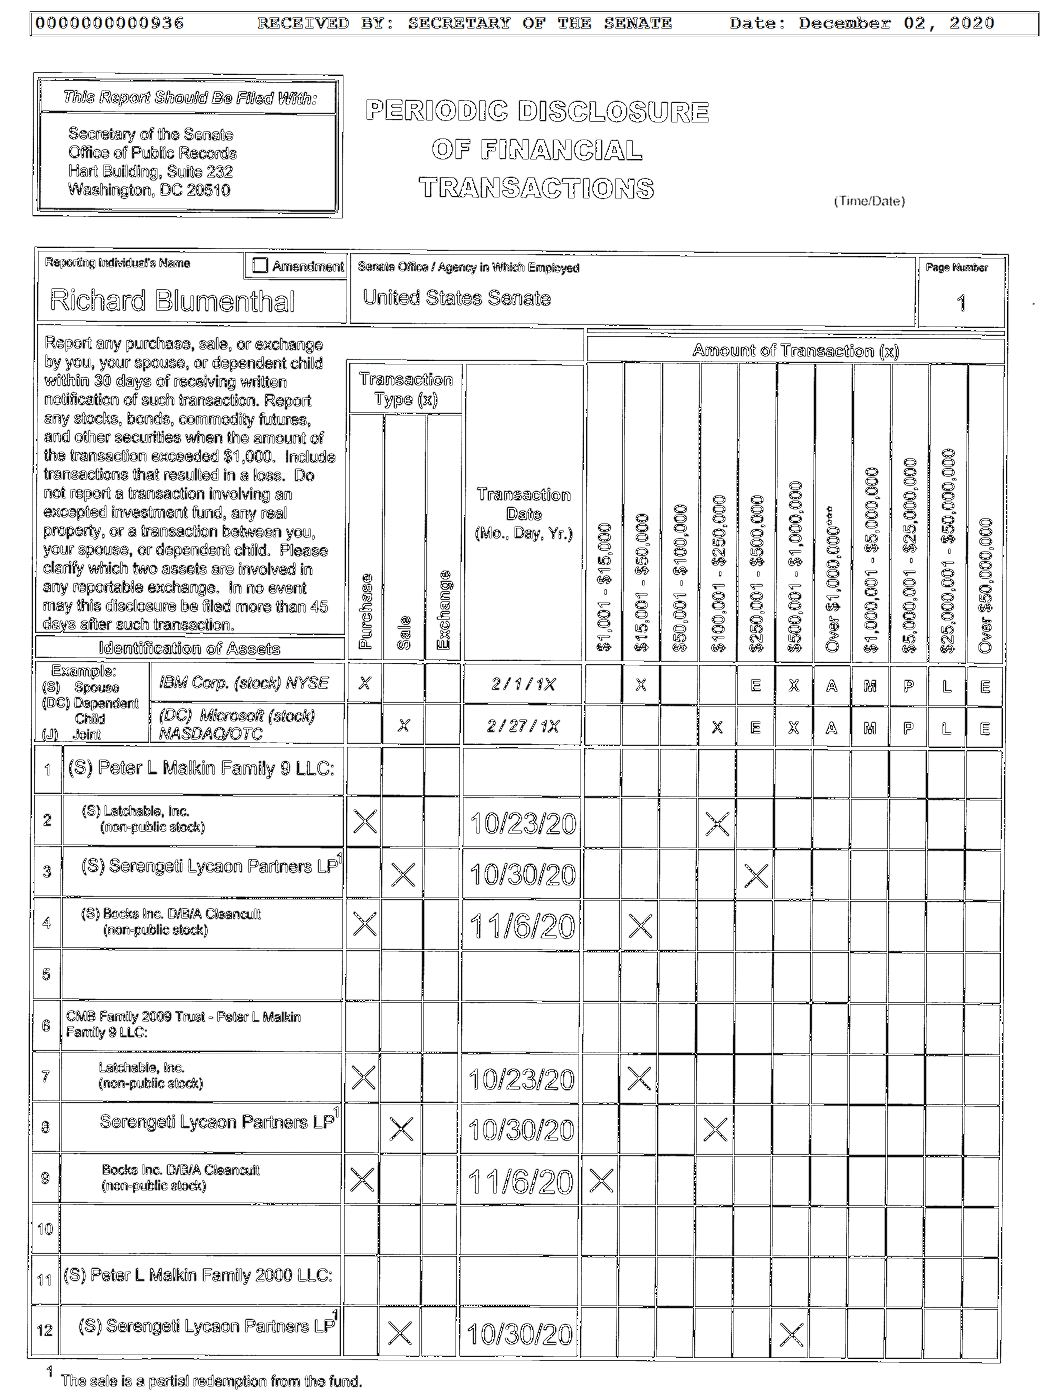
\includegraphics[width=0.52\linewidth,height=0.42\textheight,keepaspectratio]{png/figs_deck/senat_papier_droit.png}}}\\[1.5mm]
      \badgel{socr}{papier scanné --- 373}\\[0.8mm]
      {\scriptsize image, à lire par \textbf{OCR}}
    \end{column}
  \end{columns}
\end{frame}

% ── 1f · Bilan du tri : 4 sous-corpus → 4 extracteurs (charnière avant l'Extraction) ──
\begin{frame}{1c · Bilan --- quatre sous-corpus, quatre extracteurs}
  \centering
  \vspace{2mm}
  {\footnotesize la même donnée réglementaire arrive sous \textbf{4 formats}
   (chambre × format) :}\\[2mm]
  \begin{columns}[T]
    \begin{column}{0.24\textwidth}\centering
      \colorbox{helec}{\parbox{0.94\linewidth}{\centering\vspace{0.4mm}{\color{white}\scriptsize\textbf{Chambre · PDF lisible}}\vspace{0.4mm}}}\\[1mm]
      {\scriptsize \textbf{texte}\\→ \textbf{parsing} (2b)}
    \end{column}
    \begin{column}{0.24\textwidth}\centering
      \colorbox{hocr}{\parbox{0.94\linewidth}{\centering\vspace{0.4mm}{\color{black!80}\scriptsize\textbf{Chambre · PDF scanné}}\vspace{0.4mm}}}\\[1mm]
      {\scriptsize \textbf{image}\\→ \textbf{OCR} (2b)}
    \end{column}
    \begin{column}{0.24\textwidth}\centering
      \colorbox{selec}{\parbox{0.94\linewidth}{\centering\vspace{0.4mm}{\color{white}\scriptsize\textbf{Sénat · page web}}\vspace{0.4mm}}}\\[1mm]
      {\scriptsize \textbf{texte}\\→ \textbf{lecture} (2c)}
    \end{column}
    \begin{column}{0.24\textwidth}\centering
      \colorbox{socr}{\parbox{0.94\linewidth}{\centering\vspace{0.4mm}{\color{black!80}\scriptsize\textbf{Sénat · papier scanné}}\vspace{0.4mm}}}\\[1mm]
      {\scriptsize \textbf{image}\\→ \textbf{OCR} (2c)}
    \end{column}
  \end{columns}
\end{frame}

% ════ 2 · EXTRACTION ════
\pipeslide{2}{2 · Extraction}%
  {Comment fait-on sortir des transactions d'un PDF, d'une page web, d'une image ?}%
  {les \textbf{4 voies} lues : 58\,756 + 93\,325 + 14\,813 + 4\,026 =
   \textbf{170\,920 transactions extraites} (avant dédoublonnage) --- \textbf{tous
   types d'actifs} gardés ; le tri par type ne vient qu'à l'entonnoir (7)}

% ── 2a · Les dates : ce qu'on récupère de chaque ligne ──
\begin{frame}{2a · Les dates --- trois en jeu, on n'en garde que deux}
  \centering
  \vspace{1mm}
  {\footnotesize une ligne de PTR affiche \textbf{plusieurs dates} --- avant d'extraire,
   fixons laquelle compte :}\\[2mm]
  \begin{columns}[T]
    \begin{column}{0.31\textwidth}\centering
      \colorbox{warnorange}{\parbox{0.95\linewidth}{\centering\vspace{0.4mm}{\color{white}\scriptsize\textbf{Date de TRANSACTION}}\vspace{0.4mm}}}\\[1.5mm]
      {\scriptsize \emph{dans le document} --- quand le trade a eu lieu\\[1mm]
       → \textbf{on la lit} : la seule risquée (garde-fous $+$ flag, jamais inventée)}
    \end{column}
    \begin{column}{0.31\textwidth}\centering
      \colorbox{black!45}{\parbox{0.95\linewidth}{\centering\vspace{0.4mm}{\color{white}\scriptsize\textbf{Date de NOTIFICATION}}\vspace{0.4mm}}}\\[1.5mm]
      {\scriptsize \emph{dans le document} --- quand l'élu dit avoir été prévenu\\[1mm]
       → \textbf{on la jette} : inutile pour le signal}
    \end{column}
    \begin{column}{0.31\textwidth}\centering
      \colorbox{okgreen}{\parbox{0.95\linewidth}{\centering\vspace{0.4mm}{\color{white}\scriptsize\textbf{Date de DÉPÔT} (divulgation)}\vspace{0.4mm}}}\\[1.5mm]
      {\scriptsize \emph{PAS dans le document} : la \textbf{métadonnée} du dépôt\\[1mm]
       → \textbf{on la garde} = la date \textbf{signal} (anti-look-ahead)}
    \end{column}
  \end{columns}
  \vspace{4mm}
  \choixbox{la date fiable (\textbf{dépôt}) n'est \textbf{jamais lue dans le document} ---
   elle vient de l'\textbf{index} (Chambre) ou du \textbf{listing eFD} (Sénat) ; la seule
   qu'on lit vraiment dans le document, c'est la \textbf{transaction} (déposée en médiane
   \textbf{27 j} après le trade à la Chambre, \textbf{24 j} au Sénat).}
\end{frame}

% ── 2b · Extraction Chambre, texte ──
\begin{frame}{2b · Chambre · texte --- un PDF n'est pas un tableau}
  \begin{columns}[T]
    \begin{column}{0.40\textwidth}\centering
      \clickzoom{fig_ptr_multiligne}{
\includegraphics[width=\linewidth,height=0.56\textheight,keepaspectratio]{png/figs_deck/fig_ptr_multiligne.png}}\\[0.5mm]
      {\scriptsize\color{black!60} un \textbf{PTR réel} --- \textbf{un parseur naïf en
       raterait la moitié}}
    \end{column}
    \begin{column}{0.57\textwidth}
      \badge{helec}{58\,756 lignes extraites → 58\,728 uniques}\\[2mm]
      {\footnotesize \textbf{1.} \textbf{recoller} les lignes coupées\\[1mm]
       \textbf{2.} repérer la \textbf{signature} d'une transaction : opération +
       les \textbf{2 dates imprimées} (transaction, notification) + fourchette\\[1mm]
       \textbf{3.} \textbf{rattacher} le nom d'actif (toujours là) et le ticker
       \textbf{s'il est imprimé} --- sinon récupéré en (4)}\\[2.5mm]
      {\scriptsize\color{black!60} \textbf{pas d'IA} : code déterministe}
    \end{column}
  \end{columns}
  \vspace{1.5mm}
  \choixbox{le \co{[ST]} entre crochets = \textbf{« c'est une action »}, indiqué dans le
   formulaire --- mais ce marquage \textbf{n'existe pas avant 2018} : on ne s'en sert donc
   pas pour trier, c'est le \textbf{ticker} (coté = action à garder) qui décide.}
\end{frame}

% ── 2c · Extraction Chambre, image ──
\begin{frame}{2b · Chambre · image --- l'OCR lit, \textbf{Quiver} tranche}
  \centering
  {\footnotesize un PTR scanné est une \textbf{image}. Sur \textbf{2\,424 scans} :
   \textbf{1\,649 tapés} $+$ \textbf{775 manuscrits} --- lesquels garder ?}\\[4mm]
  \begin{columns}[c]
    \begin{column}{0.38\textwidth}\centering
      \begin{minipage}[t]{0.49\linewidth}\centering
        \fcolorbox{helec}{white}{\clickzoom{scan_full_droit}{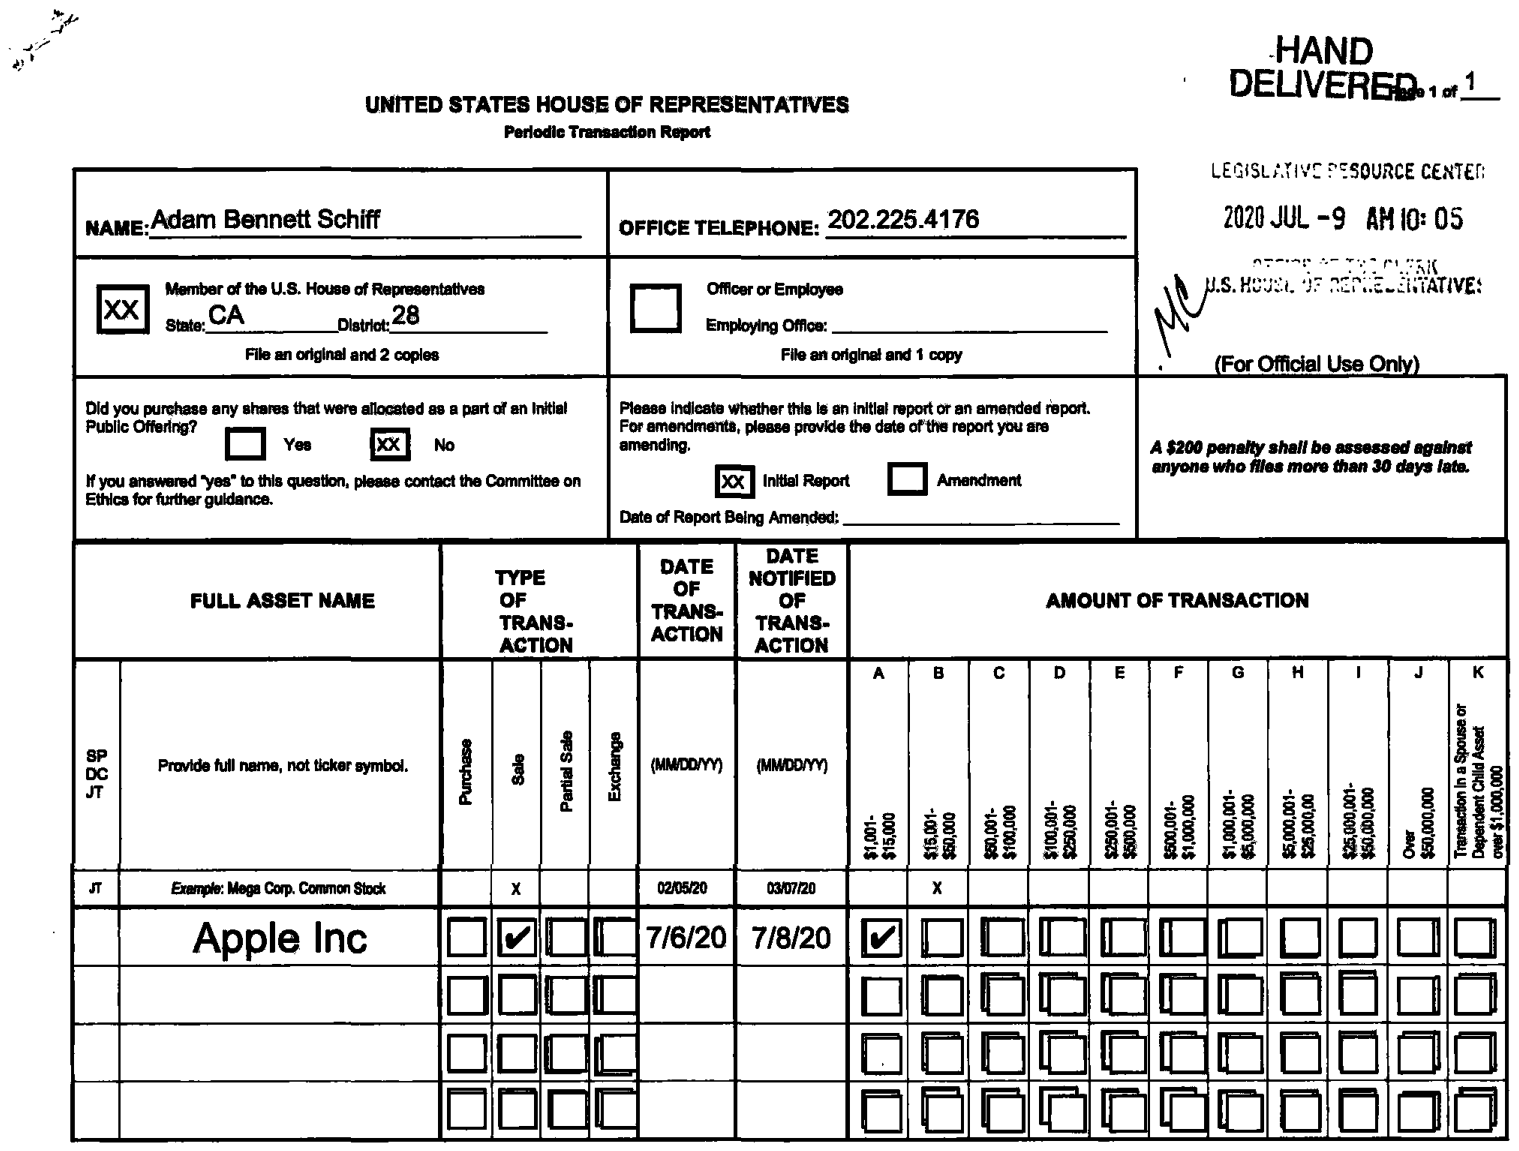
\includegraphics[width=0.9\linewidth,keepaspectratio]{png/figs_deck/scan_full_droit.png}}}\\[0.6mm]
        {\scriptsize\textbf{tapé}}
      \end{minipage}\hfill
      \begin{minipage}[t]{0.49\linewidth}\centering
        \fcolorbox{hocr}{white}{\clickzoom{scan_full_manuscrit}{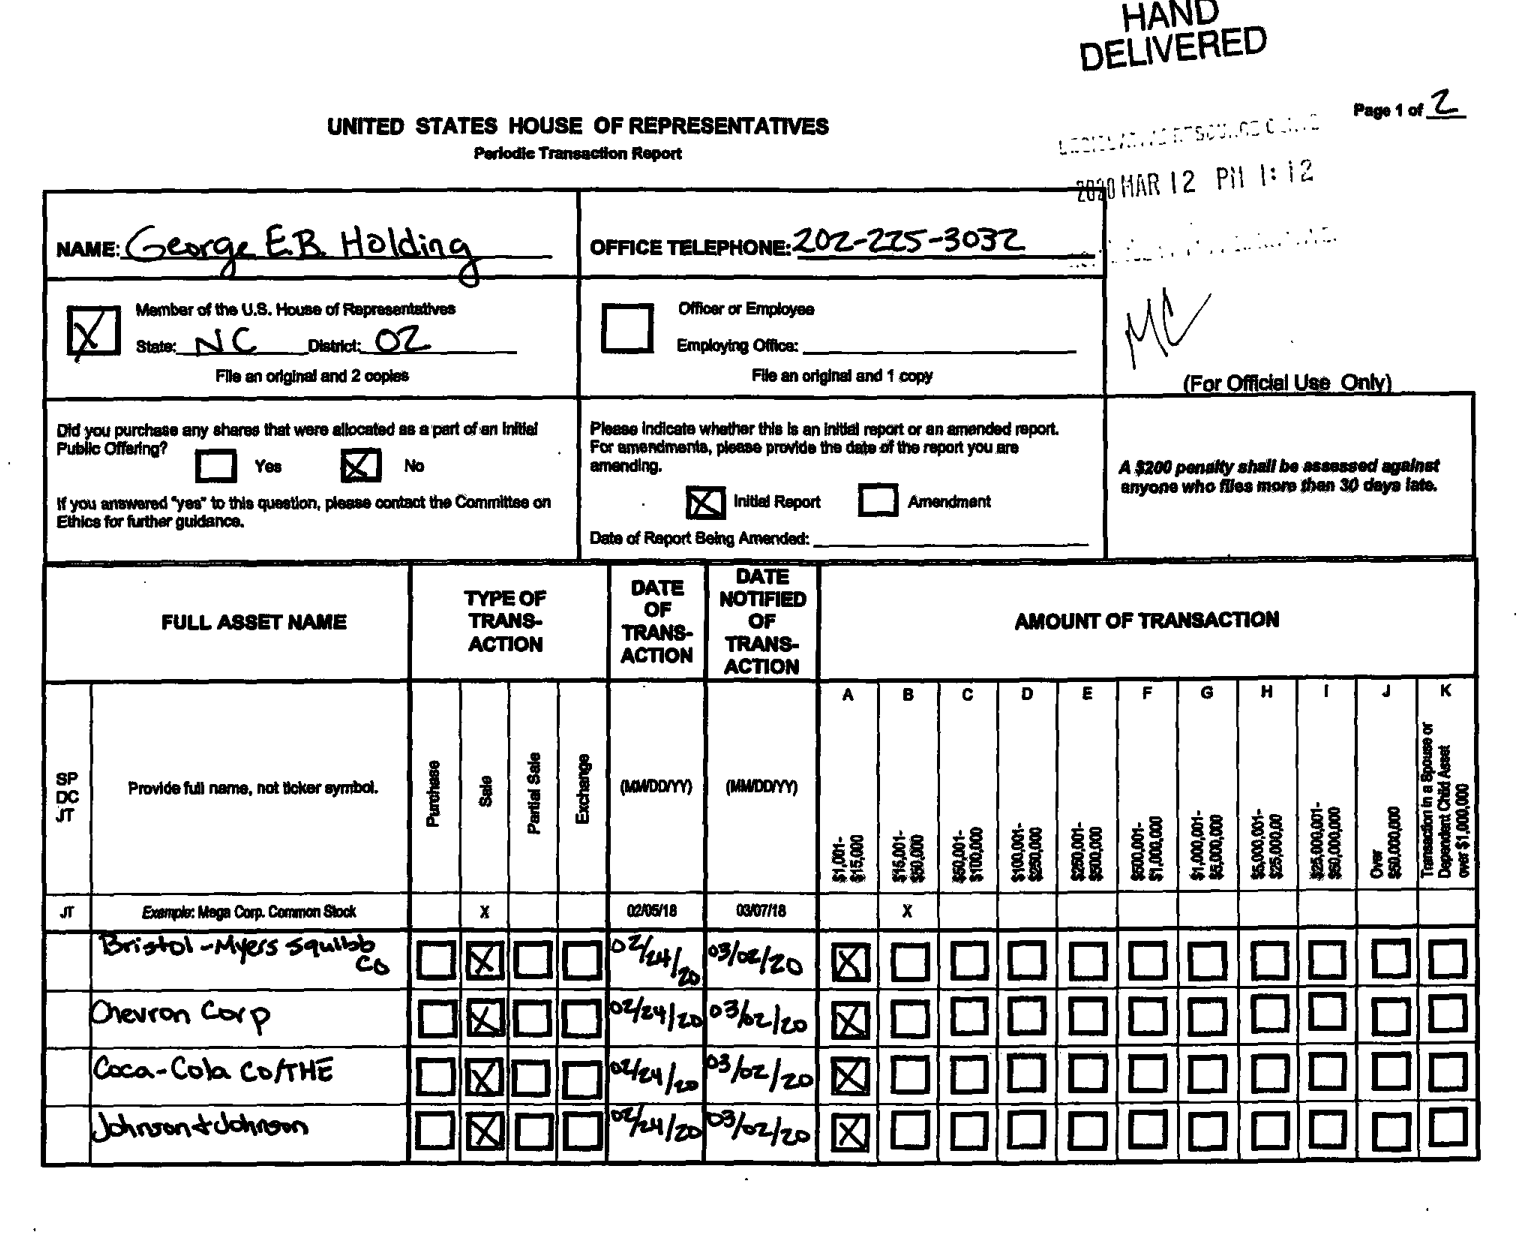
\includegraphics[width=0.9\linewidth,keepaspectratio]{png/figs_deck/scan_full_manuscrit.png}}}\\[0.6mm]
        {\scriptsize\textbf{manuscrit}}
      \end{minipage}
    \end{column}
    \begin{column}{0.58\textwidth}\centering
      {\footnotesize on compare chaque ligne à l'\textbf{ensemble Quiver} : \emph{corroborée}
       si le triplet (\textbf{élu · ticker · sens}) y figure.}\\[3mm]
      {\footnotesize\renewcommand{\arraystretch}{1.25}%
       \begin{tabular}{@{}l c c@{}}
        \toprule
        scan & corroboré & \\
        \midrule
        \textbf{tapé} · 1\,649 & \textbf{67\,\%} & \textcolor{okgreen}{\textbf{gardé}} \\
        \textbf{manuscrit} · 775 & \textbf{12,9\,\%} & \textcolor{alertred}{\textbf{écarté}} \\
        \bottomrule
      \end{tabular}}\\[3mm]
      {\footnotesize\color{black!70} exception : \textbf{193 docs} manuscrits gardés ---
       les \textbf{3 déposants} corroborés par Quiver : Schrader, Lamborn et Harshbarger.}
    \end{column}
  \end{columns}
\end{frame}

% ── 2d · Extraction Sénat, texte ──
\begin{frame}{2c · Sénat · texte --- la donnée arrive déjà en table}
  \begin{columns}[c]
    \begin{column}{0.52\textwidth}\centering
      \fcolorbox{selec}{white}{\clickzoom{senate_digital_2}{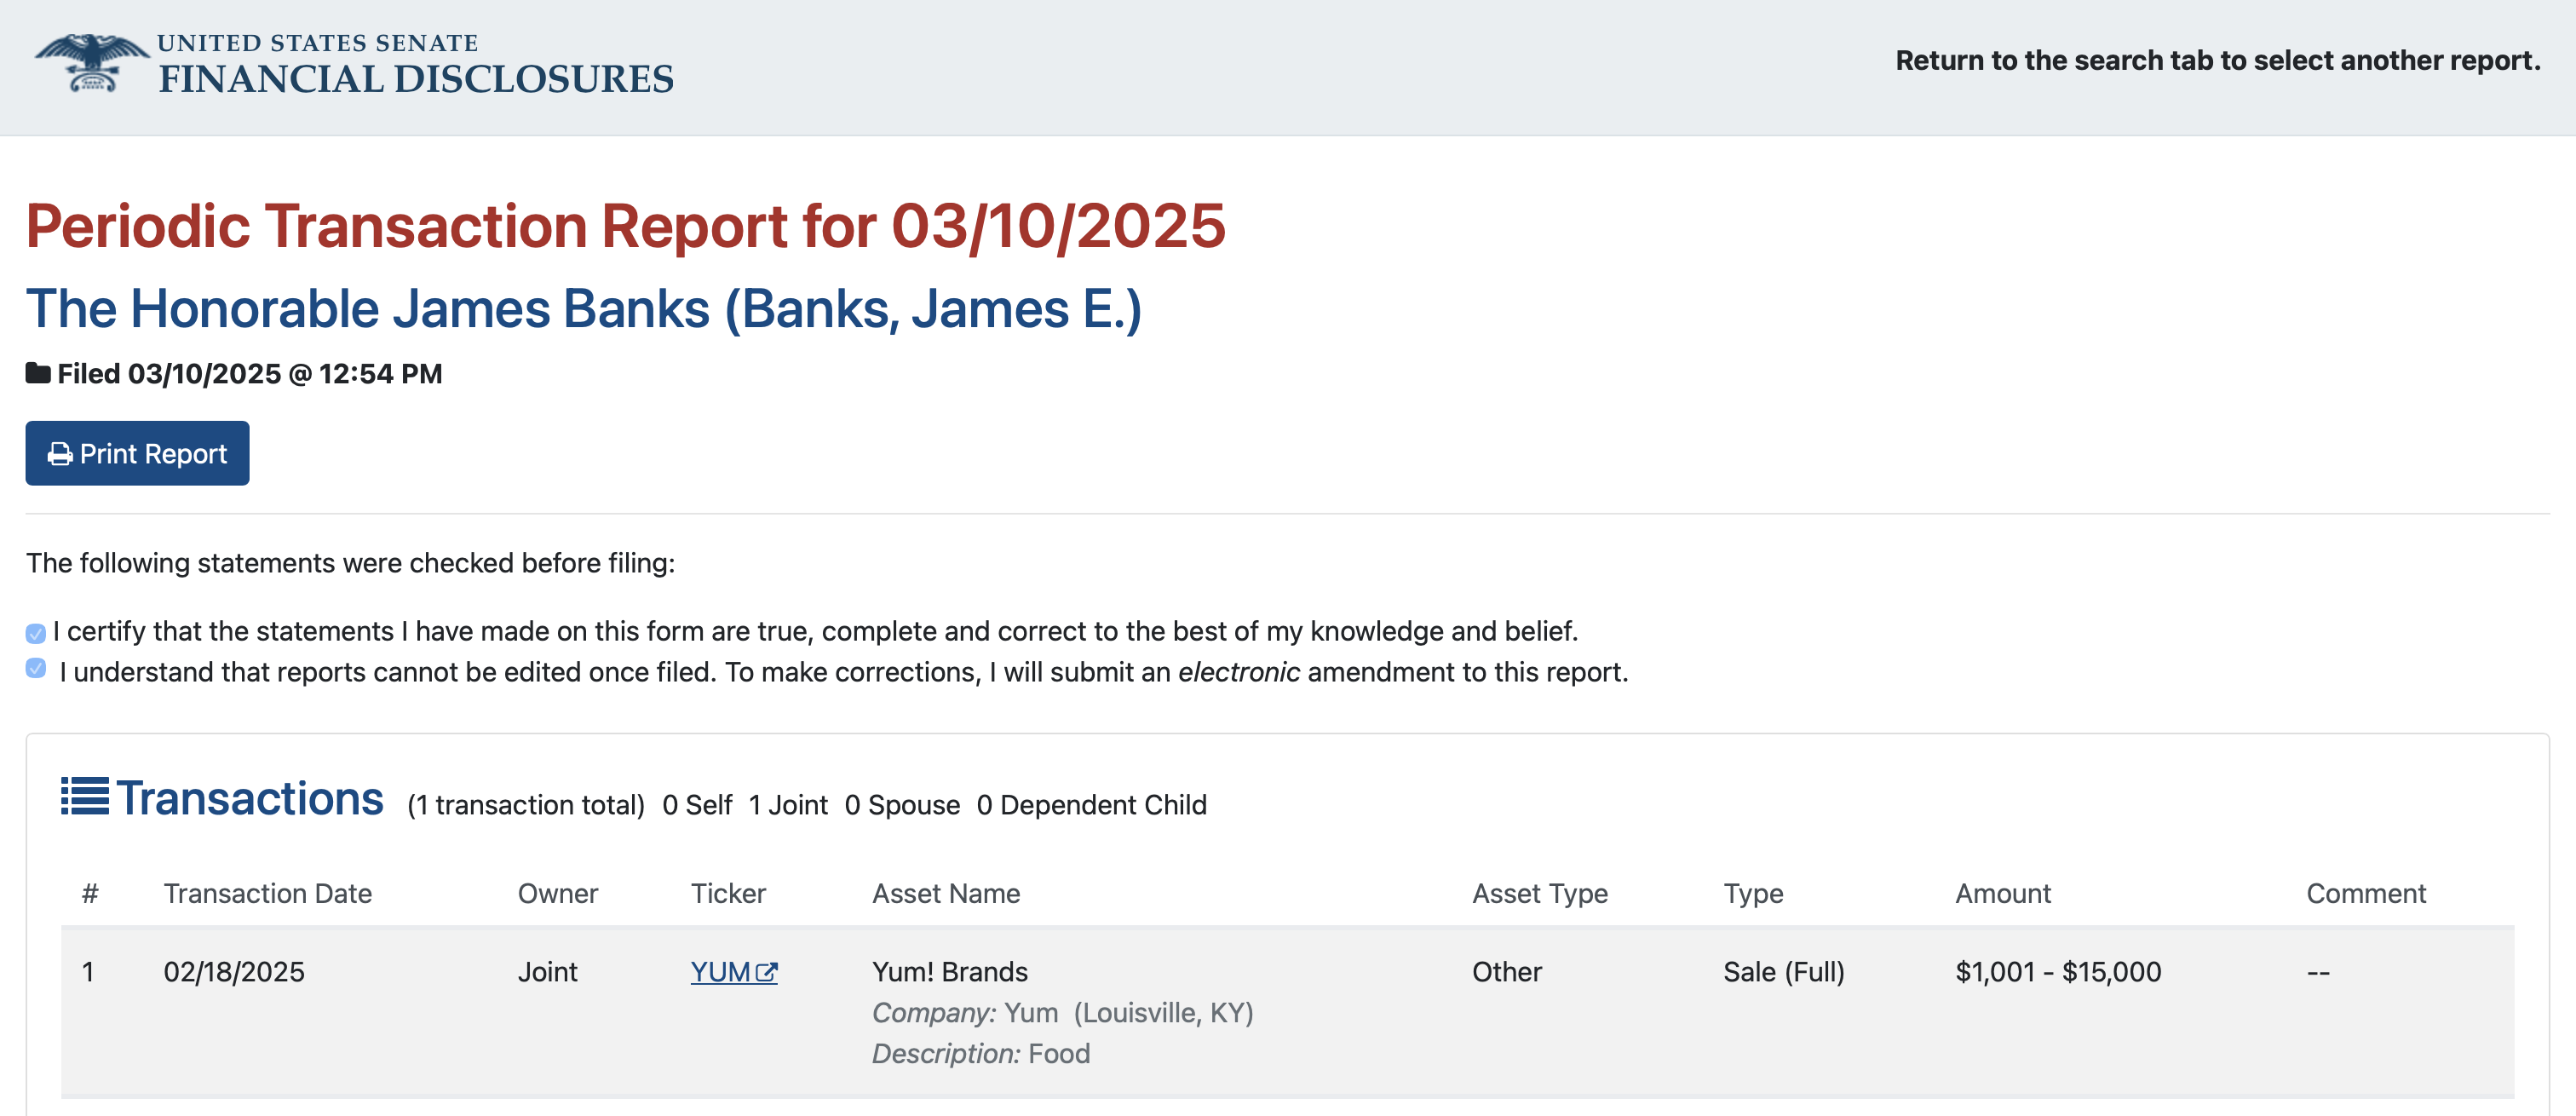
\includegraphics[width=0.96\linewidth,height=0.46\textheight,keepaspectratio]{png/figs_deck/senate_digital.png}}}
    \end{column}
    \begin{column}{0.44\textwidth}
      \badge{selec}{14\,813 lignes → 13\,026 uniques}\\[2.5mm]
      {\footnotesize chaque dépôt est une \textbf{page HTML} : on lit les \textbf{colonnes
       par leurs intitulés} --- gabarit \textbf{stable 2014→2026}, donc \textbf{déterministe
       et sans IA}. Rien à reconstruire.}\\[2.5mm]
      {\scriptsize\color{black!55} l'écart ($-12$\,\%) = re-déclarations annuelles,
       dédoublonnées en (6)}
    \end{column}
  \end{columns}
\end{frame}

% ── Le papier Sénat : composition (galerie des 3 écritures, avant 2e) ──
\begin{frame}{2c · Sénat · image --- le papier, trois écritures}
  \centering
  {\footnotesize un seul formulaire depuis 2014, mais \textbf{trois écritures} du papier ---
   classées au \textbf{Vision}, comptes recoupés avec la sortie OCR :}\\[4.5mm]
  \begin{columns}[T]
    \begin{column}{0.30\textwidth}\centering
      \parbox[t][37mm][c]{\linewidth}{\centering\fcolorbox{socr}{white}{\clickzoom{sp_tape}{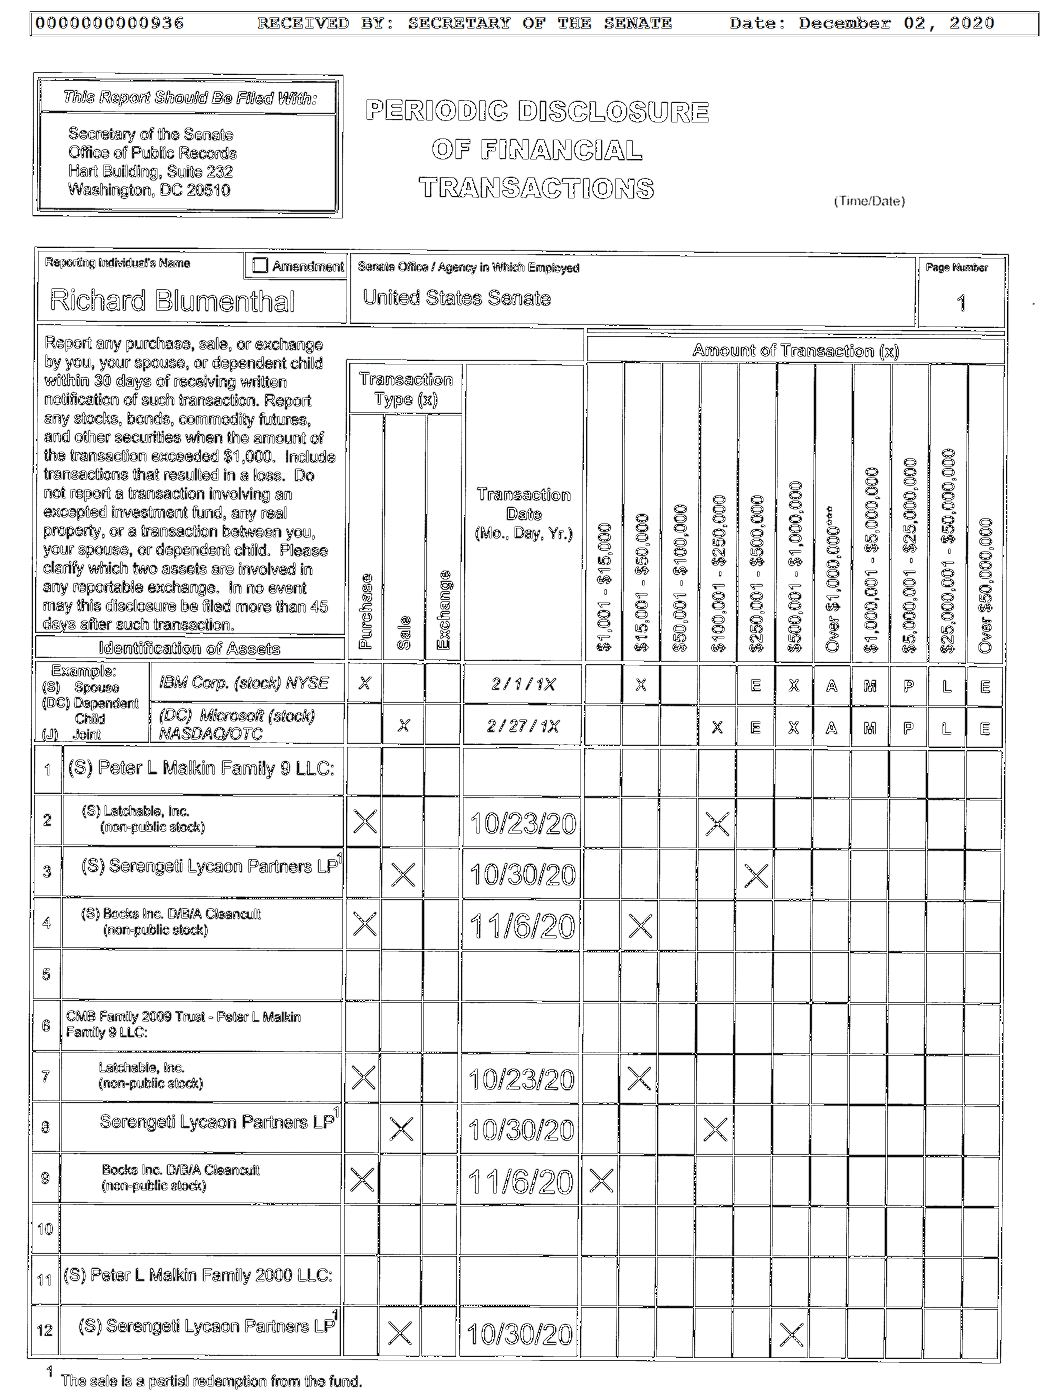
\includegraphics[width=0.8\linewidth,height=35mm,keepaspectratio]{png/figs_deck/senat_papier_droit.png}}}}\\[1.5mm]
      {\scriptsize\textbf{tapé}}\\[0.4mm]{\textbf{254}~{\scriptsize\color{black!55}69\,\%}}
    \end{column}
    \begin{column}{0.30\textwidth}\centering
      \parbox[t][37mm][c]{\linewidth}{\centering\fcolorbox{socr}{white}{\clickzoom{sp_manu}{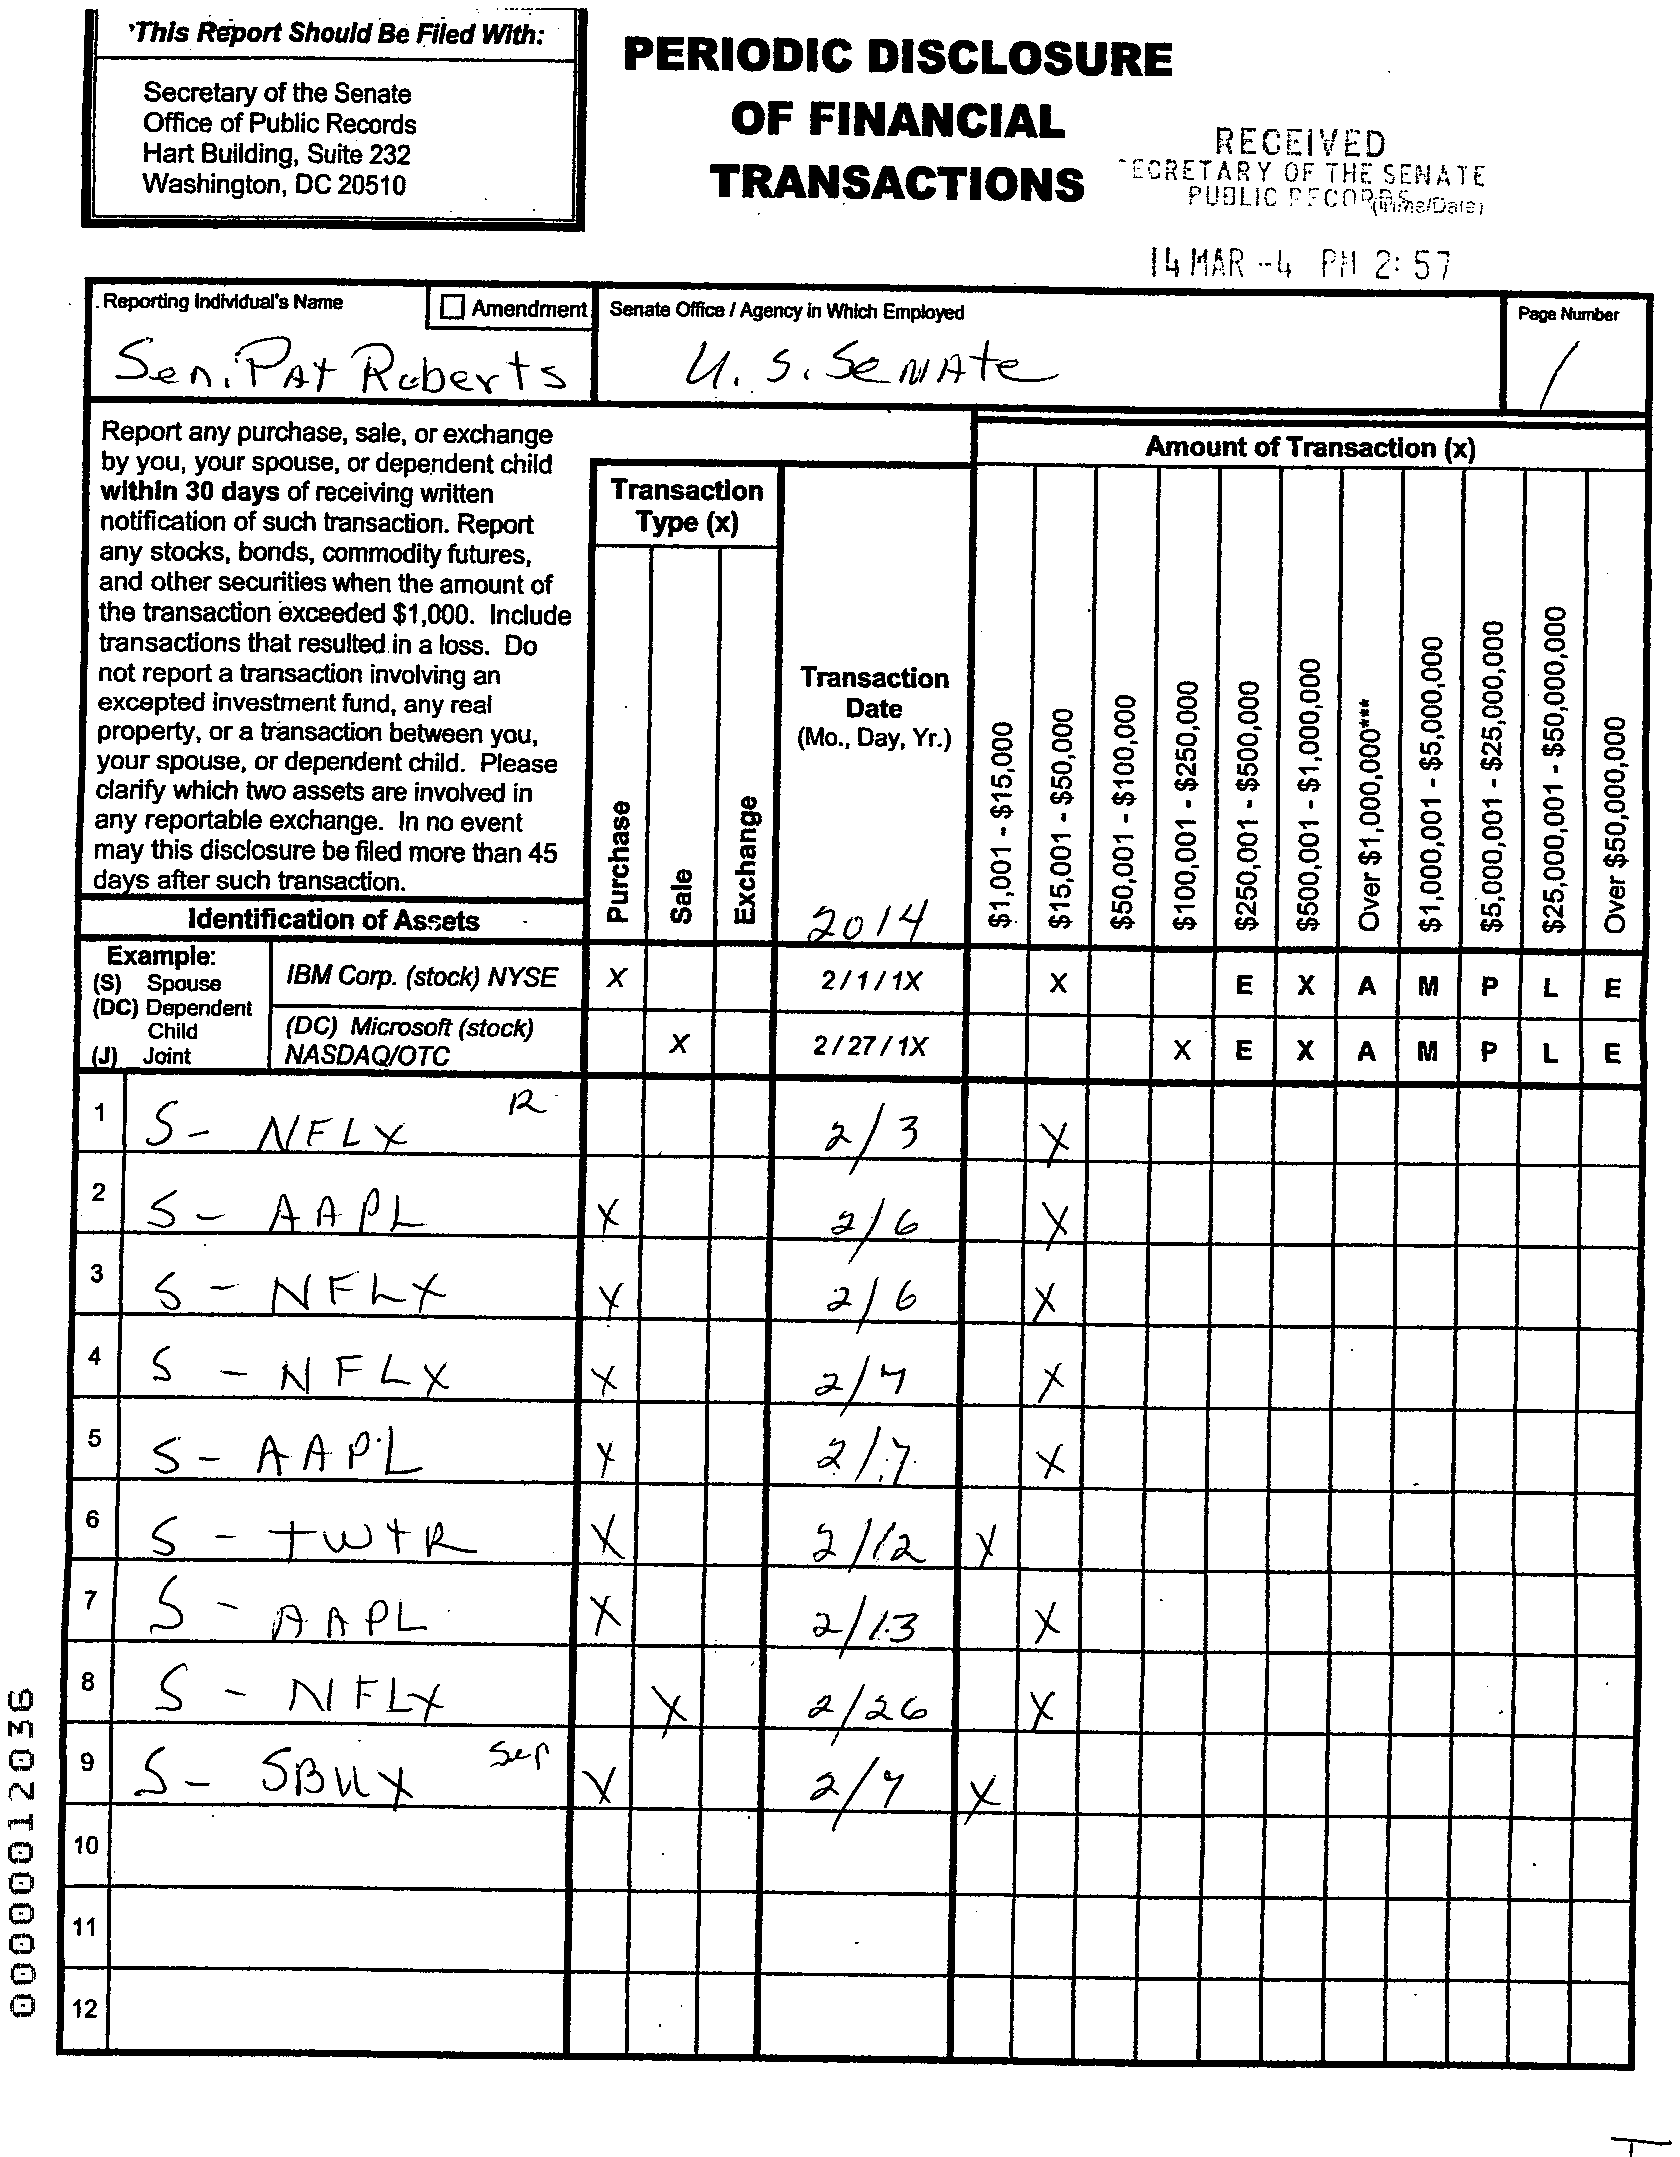
\includegraphics[width=0.8\linewidth,height=35mm,keepaspectratio]{png/figs_deck/senat_papier_manuscrit.png}}}}\\[1.5mm]
      {\scriptsize\textbf{manuscrit}}\\[0.4mm]{\textbf{11}~{\scriptsize\color{black!55}3\,\%}}
    \end{column}
    \begin{column}{0.30\textwidth}\centering
      \parbox[t][37mm][c]{\linewidth}{\centering\fcolorbox{socr}{white}{\clickzoom{sp_annexe}{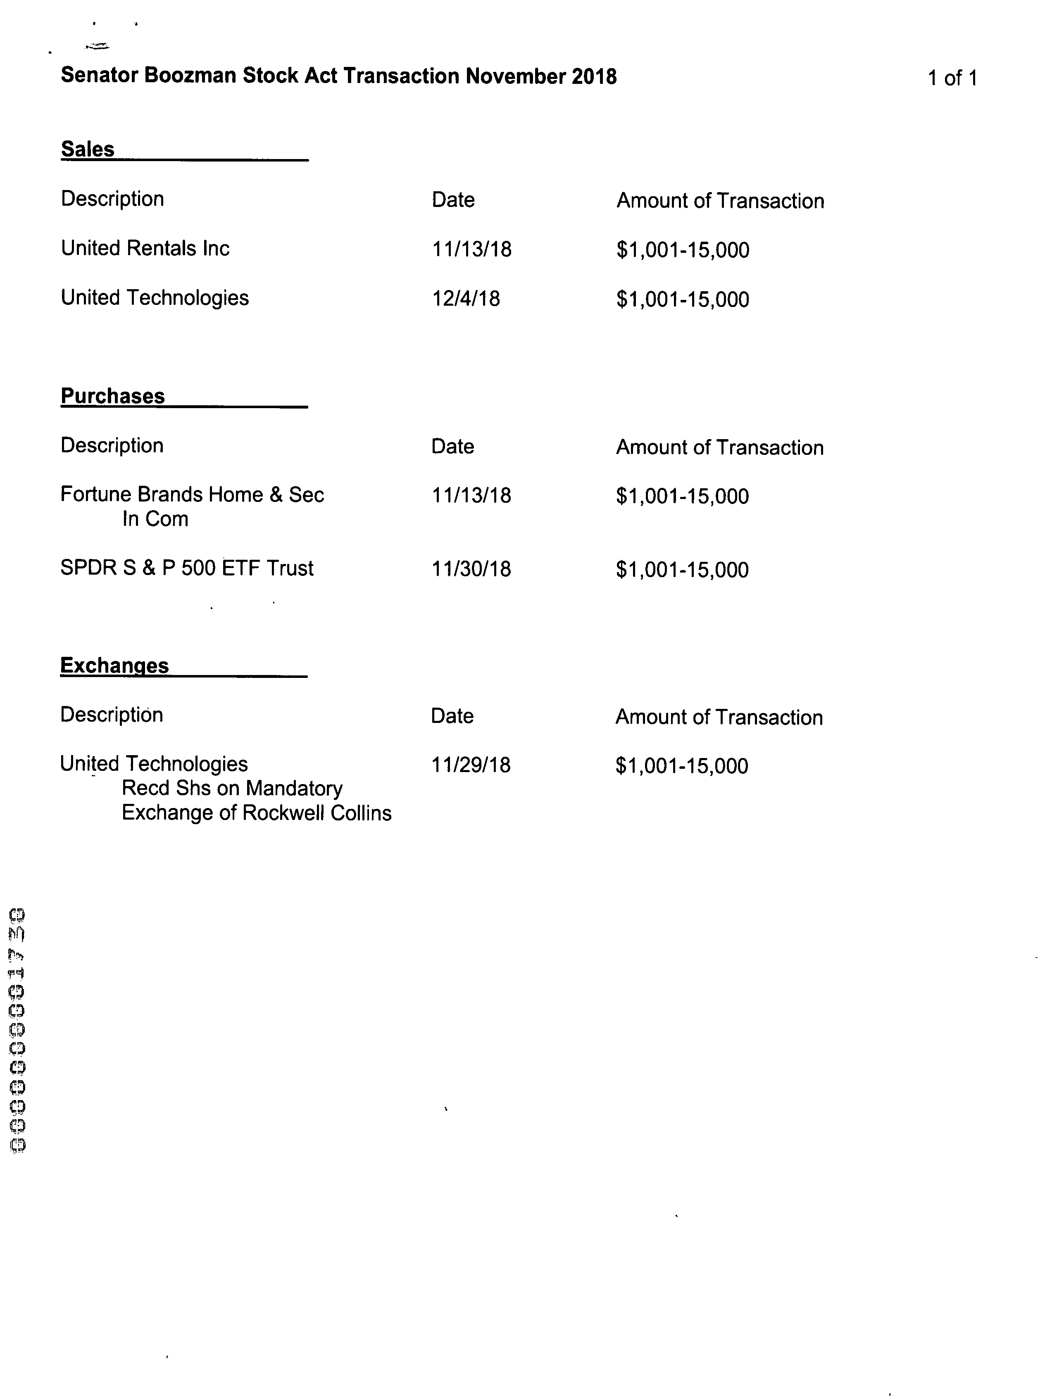
\includegraphics[width=0.8\linewidth,height=35mm,keepaspectratio]{png/figs_deck/senat_papier_annexe_v.png}}}}\\[1.5mm]
      {\scriptsize\textbf{annexe courtier}}\\[0.4mm]{\textbf{101}~{\scriptsize\color{black!55}28\,\%}}
    \end{column}
  \end{columns}
  \vspace{4.5mm}
  {\footnotesize les \textbf{trois écritures} portent les \textbf{3\,985 transactions} du papier
   Sénat (\textbf{2,4\,\%} du corpus).}
\end{frame}

% ── 2e · Extraction Sénat, image ──
\begin{frame}{2c · Sénat · image --- Quiver ne peut rien vérifier, donc on garde tout}
  \begin{columns}[c]
    \begin{column}{0.42\textwidth}\centering
      \fcolorbox{black!30}{white}{\clickzoom{senat_papier_droit_2}{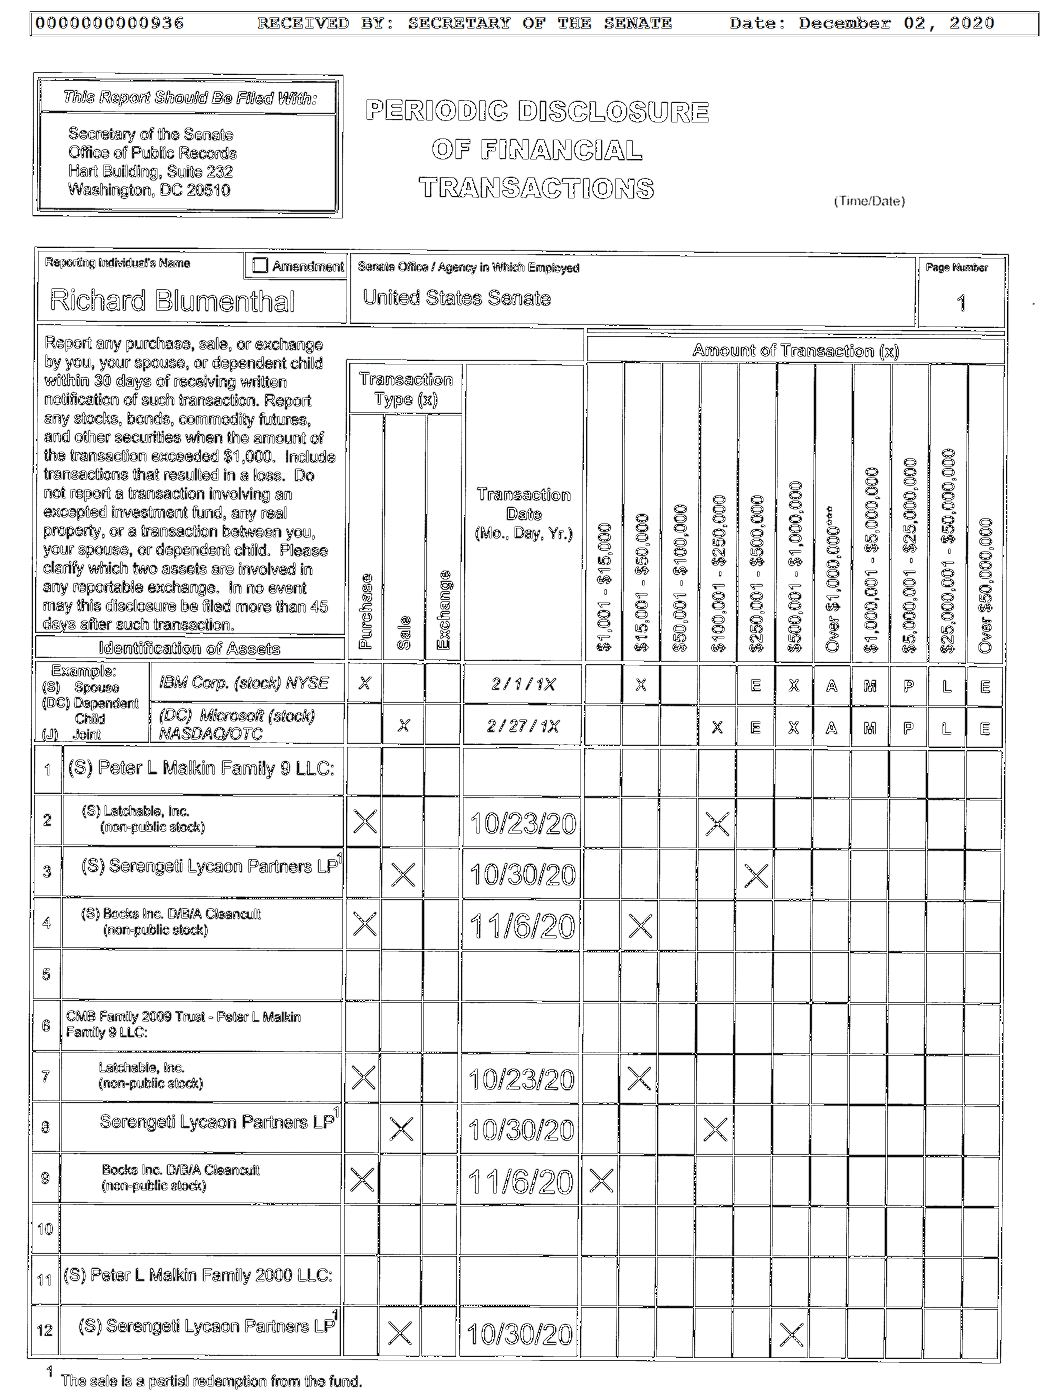
\includegraphics[width=0.92\linewidth,height=0.60\textheight,keepaspectratio]{png/figs_deck/senat_papier_droit.png}}}\\[0.6mm]
      {\scriptsize\color{black!60} papier Blumenthal (\textbf{38,7\,\%} de la voie) --- actifs
       \textbf{non cotés} : LLC, parts privées}
    \end{column}
    \begin{column}{0.54\textwidth}
      \badgel{socr}{3\,985 lignes --- 14 déposants --- 2,4\,\% du corpus}\\[2.5mm]
      {\footnotesize \textbf{Quiver n'a que des actions cotées}. Or le papier Sénat est
       \textbf{surtout du non-coté} ($\sim$60\,\% : LLC, munis) --- hors de son
       périmètre.}\\[2.5mm]
      \colorbox{socr!35}{\parbox{0.96\linewidth}{\footnotesize\vspace{0.5mm}
        et même le \textbf{coté} (40\,\%) n'apparaît pas chez Quiver : \textbf{0\,\% du
        papier retrouvé} (mesuré, chaque année) → aucun mètre externe → on \textbf{garde
        tout}. À la Chambre, à l'inverse, le papier est du coté que \textbf{Quiver possède}
        (Khanna) → on \textbf{mesure} et on écarte le manuscrit (12,9\,\%).\vspace{0.5mm}}}
    \end{column}
  \end{columns}
\end{frame}

% (slide « Le corpus extrait » déplacée en annexe A8 : à ce stade on n'a encore ni l'identité (3)
%  ni la dédup (6), qu'elle présuppose --- Alice 2026-07-19)

% ════ 3 · IDENTITÉ ════
\pipeslide{3}{3 · Identité}%
  {À qui appartient chaque ligne, quand le formulaire n'offre qu'un nom libre ?}%
  {\textbf{100\,\%} des lignes rattachées à un élu officiel}

% ── 3 · Identité ──
\begin{frame}{3 · Identité --- un même élu, écrit de mille façons → un seul ID officiel}
  \begin{columns}[T]
    \begin{column}{0.50\textwidth}
      {\footnotesize dans le corpus, un même élu apparaît sous \textbf{plusieurs graphies} ---
       ex. \textbf{Neal Dunn} (Chambre), \textbf{5 formes} du même nom :}\\[1.5mm]
      {\scriptsize\ttfamily\color{black!75}
       Neal P. Dunn\\
       Neal Patrick Dunn MD, FACS\\
       Neal Patrick Dunn, MD, FACS\\
       Neal Patrick MD, FACS Dunn\\
       Neal Patrick MD, Facs Dunn}\\[2mm]
      \centering{\Large\color{okgreen}$\Downarrow$}\\[1.5mm]
      \colorbox{okgreen}{\parbox{0.86\linewidth}{\centering\vspace{0.4mm}
        {\color{white}\textbf{\co{D000628}} · Neal Dunn}\vspace{0.4mm}}}\\[1.5mm]
      {\scriptsize\color{black!60} un seul \textbf{bioguide} --- l'identifiant officiel unique
       de l'élu au Congrès}
    \end{column}
    \begin{column}{0.46\textwidth}
      {\footnotesize on relie chaque nom à son bioguide via l'\textbf{annuaire public
       \emph{congress-legislators}} (noms, surnoms, parti, commissions), en cascade :}\\[2mm]
      {\footnotesize
       \textbf{1.} \textbf{nettoyer} le nom --- accents, titres (\emph{Hon., Dr.}),
       suffixes (\emph{Jr, III}), surnoms\\[0.8mm]
       \textbf{2.} \textbf{correspondance exacte} dans l'annuaire\\[0.8mm]
       \textbf{3.} repli \textbf{nom de famille} s'il ne désigne qu'un élu \;·\; au \senat{},
       désambiguïsation en plus (chambre, titulaire en exercice)}\\[3mm]
      \badge{okgreen}{100\,\% des lignes rattachées}\\[1.2mm]
      {\footnotesize \textbf{367} élus Chambre · \textbf{78} Sénat --- avec leur \textbf{parti}
       et leurs \textbf{commissions}}
    \end{column}
  \end{columns}
\end{frame}

% ════ 4 · TICKERS ════
\pipeslide{4}{4 · Tickers}%
  {« Apple Computer Inc » : comment retrouver le symbole boursier derrière un nom écrit à la main ?}%
  {le ticker sur \textbf{84,1\,\%} des lignes Chambre · \textbf{77,9\,\%} Sénat}

% ── 4 · Tickers ──
\begin{frame}{4 · Tickers --- d'où vient le symbole boursier, et comment il évolue}
  \centering
  \vspace{0.5mm}
  {\footnotesize \textbf{d'où vient le ticker de chaque ligne ?} \; (du plus sûr au moins sûr)}\\[2mm]
  {\scriptsize\renewcommand{\arraystretch}{1.05}%
   \begin{tabular}{@{}l >{\raggedright\arraybackslash}p{9.5cm} r@{}}
    \toprule
    \textbf{source} & \textbf{exemple} & \textbf{part} \\
    \midrule
    \textbf{explicite} & imprimé dans le document, à côté du nom : «\,Apple Inc \textbf{(AAPL)}\,» --- on le \textbf{lit} & \textbf{38\,\%} \\
    \textbf{dictionnaire} & «\,nom = ticker\,» \textbf{appris de l'électronique}, réappliqué au papier : «\,Microsoft Corp\,» → \textbf{MSFT} & \textbf{21\,\%} \\
    \textbf{IA (Claude)} & on interroge l'\textbf{API Claude} : «\,Palantir\,» → \textbf{PLTR} (si cotée) ; une passe \textbf{vérifiée} rattrape ses oublis & \textbf{24,5\,\%} \\
    \emph{aucun} & actif \textbf{non coté} (obligation, LLC privée) --- pas de ticker & \textbf{16,5\,\%} \\
    \bottomrule
  \end{tabular}}\\[3mm]
  {\footnotesize \textbf{et le symbole peut changer dans le temps} \; --- \textbf{84 cas} suivis}\\[2mm]
  {\scriptsize\renewcommand{\arraystretch}{1.05}%
   \begin{tabular}{@{}l >{\raggedright\arraybackslash}p{8.2cm} r@{}}
    \toprule
    \textbf{le changement} & \textbf{→ le prix} & \textbf{cas} \\
    \midrule
    \textbf{renommée / fusionnée} & nouveau symbole (Facebook → \textbf{META}) → \textbf{prix continu} & \textbf{32} \\
    \textbf{rachetée / faillite} & quitte la Bourse (Twitter → X, privé) → \textbf{délisté} & \textbf{48} \\
    \textbf{symbole recyclé} & mêmes lettres, 2 sociétés (Hertz réémis) → prix \textbf{par période} & \textbf{4} \\
    \bottomrule
  \end{tabular}}
\end{frame}

% ════ 5 · SECTEURS ════
\pipeslide{5}{5 · Secteurs}%
  {Dans quel secteur joue chaque titre --- et par quel panier coté peut-on l'approcher ?}%
  {le secteur sur \textbf{79,8\,\%} des lignes Chambre · \textbf{70,4\,\%} Sénat}

% ── 5 · Secteurs ──
\begin{frame}{5 · Secteurs --- chaque action : un secteur, puis son ETF}
  \centering
  {\footnotesize Investir \textbf{par secteur} = acheter l'\textbf{ETF} du secteur. On traduit donc chaque action :}\\[1mm]
  \begin{tikzpicture}[node distance=6mm]
    \node[bande=helec, text width=2.8cm, align=center] (a) {« Apple Inc »\\[0.2mm]\co{AAPL}};
    \node[bande=dataC, text width=3.4cm, align=center, right=of a] (b)
      {\textbf{Information Technology}\\[0.2mm]{\scriptsize 1 des 11 secteurs GICS}};
    \node[bande=okgreen, text width=2.9cm, align=center, right=of b] (c)
      {ETF \textbf{XLK}\\[0.2mm]{\scriptsize le fonds coté du secteur}};
    \draw[arr] (a) -- (b); \draw[arr] (b) -- (c);
  \end{tikzpicture}\\[0.5mm]
  {\scriptsize\color{black!70} contre-exemple : « obligation municipale » → \textbf{non cotée} →
   \textbf{aucun secteur} (par nature, pas un raté)}\\[0.5mm]
  \begin{columns}[T]
    \begin{column}{0.53\textwidth}\footnotesize
      \textbf{d'où vient le secteur} de chaque ligne ? 3 méthodes, en cascade :\\[1.5mm]
      {\renewcommand{\arraystretch}{1.1}%
       \begin{tabular}{@{}>{\raggedright\arraybackslash}p{5.7cm}r@{}}
        \toprule \textbf{méthode} & \textbf{part} \\ \midrule
        \textbf{base boursière} (Yahoo Finance) --- le secteur officiel de l'entreprise & $\approx$67\,\% \\
        \textbf{IA} (Claude) --- si absent : choisit 1 des 11 secteurs, refuse si non coté & $\approx$12\,\% \\
        \textbf{à la main} --- quelques cas connus (ex.\ l'ETF SPY : pas de secteur) & $<$1\,\% \\
        \bottomrule
      \end{tabular}}\\[1.5mm]
      \badge{dataC}{secteur = ETF renseigné}\quad{\footnotesize \textbf{79,8\,\%} Ch.\ · \textbf{70,4\,\%} Sén.}
    \end{column}
    \begin{column}{0.45\textwidth}\footnotesize
      \textbf{GICS} = la nomenclature boursière : \textbf{11 secteurs}, chacun avec \textbf{un}
      ETF SPDR \emph{Select Sector} :\\[1mm]
      {\ttfamily\footnotesize Energy→XLE · Materials→XLB · Industrials→XLI · Cons.\ Discr.→XLY ·
       Cons.\ Staples→XLP · Health Care→XLV · Financials→XLF · Info.\ Tech.→XLK ·
       Comm.\ Services→XLC · Utilities→XLU · Real Estate→XLRE}
    \end{column}
  \end{columns}
\end{frame}

% ════ 6 · DÉDUP ════
\pipeslide{6}{6 · Dédup}%
  {Un trade re-déclaré dans un amendement : comment le compter une fois --- sans effacer les vrais lots ?}%
  {\textbf{169\,000} transactions uniques (170\,920 lignes brutes, \textbf{−1\,920})}

% ── 6 · Dédup ──
\begin{frame}{6 · Dédup --- une transaction = 7 champs : l'empreinte dédoublonne sans détruire}
  \begin{columns}[T]
    \begin{column}{0.55\textwidth}\footnotesize
      \textbf{les 7 champs} :\\
      {\scriptsize \textbf{qui} (déclarant) · \textbf{quand} (date du trade) ·
       \textbf{quoi} (actif) · \textbf{sens} · \textbf{montant} (fourchette) ·
       \textbf{pour qui} (détenteur) · \textbf{chambre}}\\[2mm]
      {\scriptsize elle exclut \textbf{délibérément} :\\
       · le \textbf{ticker} --- ajouté après coup (4), sa présence rendrait
         l'empreinte instable\\
       · la \textbf{date de divulgation} --- un dépôt et son amendement portent le
         \emph{même} trade → une seule transaction}\\[2.5mm]
      \choixbox{dédup \textbf{non destructrice} : deux dépôts de même empreinte = un seul
       trade ; un \textbf{vrai lot répété} (même titre, plusieurs comptes) reste
       \textbf{distingué par un compteur d'occurrence}.}
    \end{column}
    \begin{column}{0.43\textwidth}
      \centering
      \begin{tikzpicture}[node distance=3mm]
        \node[bande=grisC, text width=4.9cm] (a) {\textbf{170\,920} lignes brutes (× 28 col.)};
        \node[bande=grisC, text width=4.9cm, below=of a] (b) {re-divulgations dédoublonnées \textbf{−1\,920}};
        \node[bande=dataC, fill=dataC!14, text width=4.9cm, below=of b] (c)
          {\textbf{169\,000 transactions uniques}};
        \draw[arr] (a) -- (b); \draw[arr] (b) -- (c);
      \end{tikzpicture}\\[2mm]
      \idem{\scriptsize \textbf{une seule empreinte} pour les deux chambres --- c'est
       elle qui permet de \textbf{fusionner les 4 voies} sans compter deux fois.}
    \end{column}
  \end{columns}
\end{frame}

% ════ 7 · ENTONNOIR ════
\pipeslide{7}{7 · Entonnoir}%
  {Un backtest exige un prix de marché : que faut-il retirer, et sur quelle preuve ?}%
  {\textbf{deux entonnoirs} --- les \textbf{lignes} (169\,000 → \textbf{134\,464} exploitables),
   puis les \textbf{symboles} (\textbf{3\,289} avec un prix) → \textbf{118\,029} trades
   \textbf{backtestables} : le livrable}

% ── 7a · Entonnoir ──
\begin{frame}{7a · Entonnoir des lignes --- de 169\,000 à 134\,464 : on ne retire que l'avéré inutilisable}
  \begin{columns}[T]
    \begin{column}{0.58\textwidth}
      \centering
      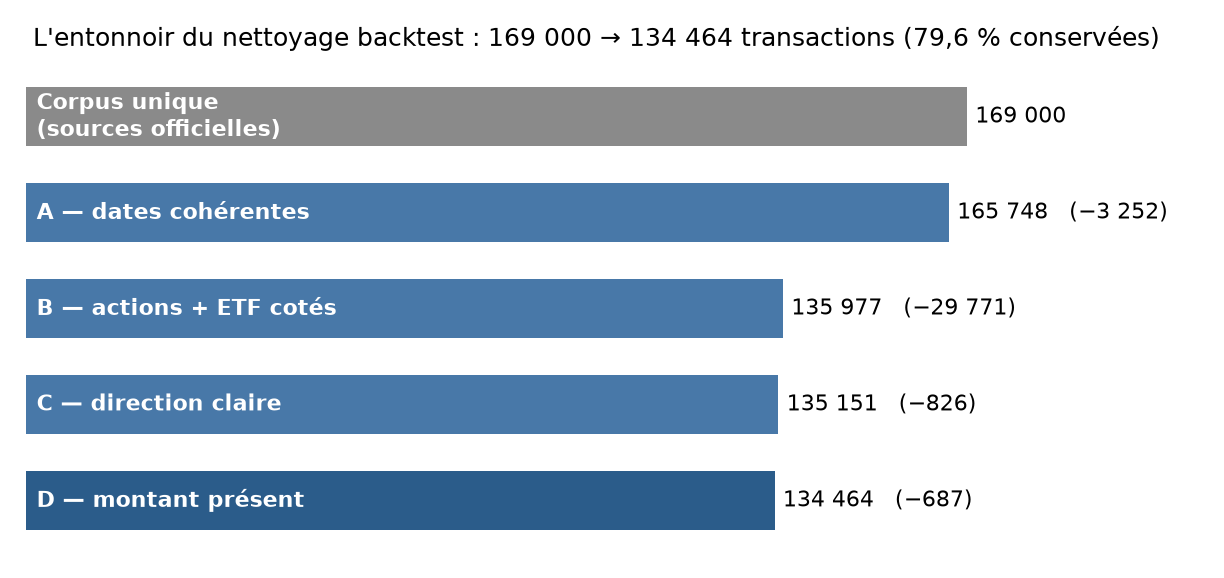
\includegraphics[width=\linewidth]{png/figs_deck/entonnoir_backtest.png}
    \end{column}
    \begin{column}{0.40\textwidth}
      {\footnotesize \textbf{quatre portes} --- ce que chacune vérifie :}\\[1mm]
      {\scriptsize
      \textbf{A · dates cohérentes} : divulgation \textbf{après} la transaction (sinon impossible), année plausible\\[0.6mm]
      \textbf{B · actions/ETF cotés} : ticker \textbf{vraiment coté} (pas obligation/muni/option) --- \textbf{gros filtre} (−29\,771)\\[0.6mm]
      \textbf{C · sens clair} : \textbf{achat ou vente} (pas un échange)\\[0.6mm]
      \textbf{D · montant présent} : la \textbf{fourchette} est renseignée}\\[2mm]
      \colorbox{okgreen!10}{\parbox{0.96\linewidth}{\scriptsize
        \textbf{\textcolor{okgreen}{sauvetage « ticker-first »}} --- \textbf{21\,878}
        lignes à case « type d'actif » vide \textbf{gardées} : le \textbf{ticker coté}
        fait foi, pas la case déclarée}}
    \end{column}
  \end{columns}
  \vspace{1.5mm}
  \centering
  \choixbox{on ne retire que l'\textbf{avéré inutilisable} ; le doute est
   \textbf{flagué, jamais retiré} (late filing 12,2\,\%, délistés, lots multi-comptes).}
\end{frame}

% ── 7b · Du symbole au prix ──
\begin{frame}{7b · Entonnoir des symboles --- 118\,029 trades ont un prix fiable ($\approx$88\,\% des 134\,464)}
  \begin{columns}[T]
    \begin{column}{0.58\textwidth}
      \centering
      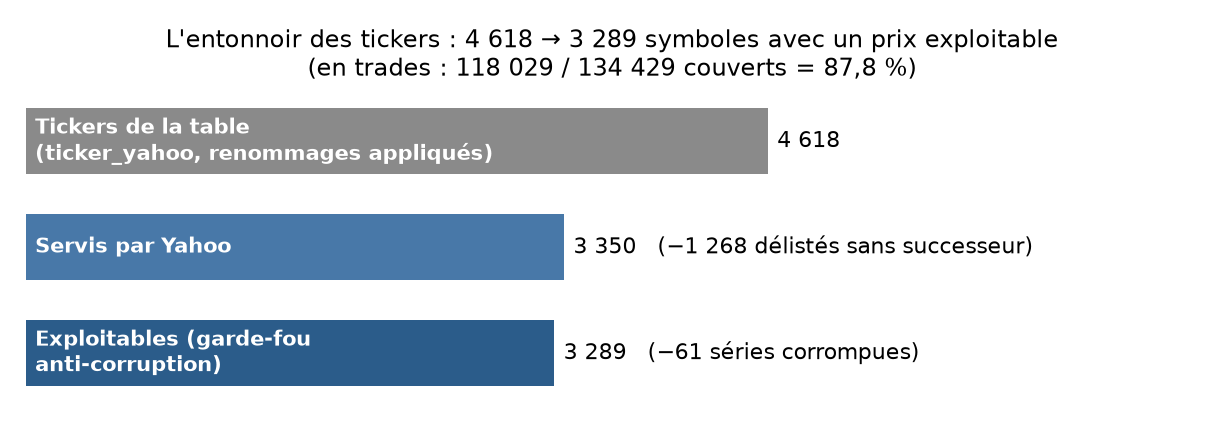
\includegraphics[width=\linewidth]{png/figs_deck/entonnoir_tickers.png}
    \end{column}
    \begin{column}{0.40\textwidth}
      {\footnotesize pour valoriser un trade, il faut un \textbf{vrai cours} --- chaque symbole est
       demandé à \textbf{Yahoo Finance} :}\\[1.5mm]
      {\scriptsize
      \textbf{délisté sans successeur} : société morte (faillite/rachat) → \textbf{plus aucun cours}\\[0.8mm]
      \textbf{série corrompue} : prix aberrants, écartés par garde-fou}\\[2.5mm]
      \badge{okgreen}{118\,029 / 134\,464 backtestables ($\approx$88\,\%)}\\[3mm]
      \colorbox{warnorange!12}{\parbox{0.96\linewidth}{\scriptsize\vspace{0.5mm}
        \textbf{\textcolor{warnorange}{biais de survie assumé}} --- on ne peut valoriser que les titres
        \textbf{encore cotés} : couverture \textbf{74\,\%} en 2014 → \textbf{99\,\%} en 2026\vspace{0.5mm}}}
    \end{column}
  \end{columns}
  \vspace{1.5mm}
  \centering
  \choixbox{les lignes sans prix restent dans le \textbf{corpus livré}, flaguées.}
\end{frame}

% ════ 8 · TABLE FINALE ════
\pipeslide{8}{8 · Table finale}%
  {Au bout du pipeline : à quoi ressemble, concrètement, une ligne livrée ?}%
  {la table de recherche --- \textbf{118\,029 trades backtestables}, limites écrites}

% ── 8 · La table finale ── (ferme la Partie I)
\begin{frame}{8 · À quoi ressemble la valeur finale : 118\,029 trades backtestables × 36 colonnes}
  \centering
  \colorbox{helec}{\parbox{0.9\textwidth}{\scriptsize\color{white}\centering\vspace{0.5mm}
    la table de recherche --- \textbf{118\,029 trades backtestables} (× 36 colonnes) ·
    372 élus · chaque ligne traçable à son document source\vspace{0.5mm}}}\\[6mm]
  {\setlength{\tabcolsep}{3.5pt}\small
  \resizebox{\textwidth}{!}{%
  \begin{tabular}{@{}lllllllrllll@{}}
    \toprule
    \textbf{membre} & \textbf{chambre} & \textbf{parti} & \textbf{comités} & \textbf{date trade} & \textbf{date div.} & \textbf{sens} & \textbf{montant \$} & \textbf{type} & \textbf{ticker} & \textbf{secteur} & \textbf{ETF} \\
    \midrule
    Bob Gibbs & House & R & Transport. & 2014-12-30 & 2015-01-26 & buy & 8\,000,5 & action & INTC & Info.\ Tech. & XLK \\
    Greg Gianforte & House & R & Ress.\ nat. & 2018-12-12 & 2019-01-14 & sell & 32\,500,5 & action & BBAVY & Cons.\ base & XLP \\
    Kim Schrier & House & D & Agriculture & 2021-11-15 & 2021-12-13 & buy & 375\,000,5 & action & AAPL & Info.\ Tech. & XLK \\
    \bottomrule
  \end{tabular}}}\\[6mm]
  {\footnotesize\textbf{12 champs garantis} sur chaque ligne, dans les 2 chambres --- chaque valeur traçable à son document source}
\end{frame}

% ══════════════════ ÉTAPE 9 · VÉRIFIER (fin de Partie I) ══════════════════
% ════ corroboration externe : Quiver + autres preuves ════

% ── Slide-repère « vous êtes ici » : étape 9 (comme les étapes 1-8) ──
\pipeslide{9}{9 · Vérifier}%
  {La table est-elle fiable ? On la confronte à des \textbf{tiers indépendants}.}%
  {corroboration externe : \textbf{Quiver} retrouvé à $>$\,92\,\%, et on en est le sur-ensemble}




% ── 9 · Quiver (on retrouve la base du tiers) ──
\begin{frame}{9 · Quiver --- nous retrouvons $>$\,92\,\% de sa base, et nous en sommes le sur-ensemble}
  \begin{columns}[c]
    \begin{column}{0.46\textwidth}\centering
      \begin{tikzpicture}
        \begin{scope}[fill opacity=0.5]
          \fill[helec!35] (0,0) circle (1.42);
          \fill[dataC!35] (1.97,0) circle (1.42);
        \end{scope}
        \draw[helec, line width=1.1pt] (0,0) circle (1.42);
        \draw[dataC, line width=1.1pt] (1.97,0) circle (1.42);
        \node[font=\footnotesize\bfseries, text=helec] at (-0.9,1.62) {NOUS (169\,000)};
        \node[font=\footnotesize\bfseries, text=dataC] at (2.9,1.62) {QUIVER};
        \node[align=center, font=\scriptsize, text width=1.5cm] at (-0.75,0)
          {\textbf{nous seuls}\\{\color{helec}\textbf{$\approx$\,26\,500}}\\{\tiny (sur-ensemble)}};
        \node[align=center, font=\scriptsize, text width=1.5cm] at (0.985,0)
          {\textbf{retrouvés}\\\mbox{\textbf{93,5\,\%} Ch.}\\\mbox{\textbf{92,1\,\%} Sén.}};
        \node[align=center, font=\scriptsize, text width=1.6cm] at (2.78,0)
          {\textbf{Quiver seul}\\\mbox{\textbf{38} → {\color{alertred}\textbf{27+11}}}\\{\tiny vrais trous documentés}};
      \end{tikzpicture}\\[1mm]
      {\scriptsize\color{black!60} au niveau (élu, ticker, sens) : \textbf{93,5\,\% /
       92,1\,\%} des combinaisons \emph{de Quiver} sont retrouvées \emph{chez nous}}
    \end{column}
    \begin{column}{0.52\textwidth}\footnotesize
      {\scriptsize\color{black!60} Quiver = fournisseur commercial des mêmes données ---
       notre mètre externe}\\[1.5mm]
      \textbf{trois crans de strictesse} --- on serre la vis :\\[1mm]
      {\scriptsize
      \badge{helec}{1 · exister} même élu, même titre, même sens\\[0.8mm]
      \badge{helec}{2 · dater} même date ($\leq$10 j) --- appariés un à un\\[0.8mm]
      \badge{helec}{3 · concorder} sens \textbf{96,8\,\%} · montant \textbf{94,2\,\%} (Chambre)}\\[2mm]
      \choixbox{Quiver est une \textbf{vérité-terrain jamais réinjectée} : il
       \textbf{mesure} la table, ne la remplit jamais --- et en cas de désaccord de
       date, \textbf{le PDF officiel arbitre toujours} (annexe A6).}
    \end{column}
  \end{columns}
\end{frame}

% ── 9 · Quiver — corroboration par année (l'autre sens : nous → Quiver) ──
\begin{frame}{9 · Quiver --- la corroboration monte avec le temps : peu de vérité-terrain avant 2017}
  \begin{columns}[c]
    \begin{column}{0.58\textwidth}\centering
      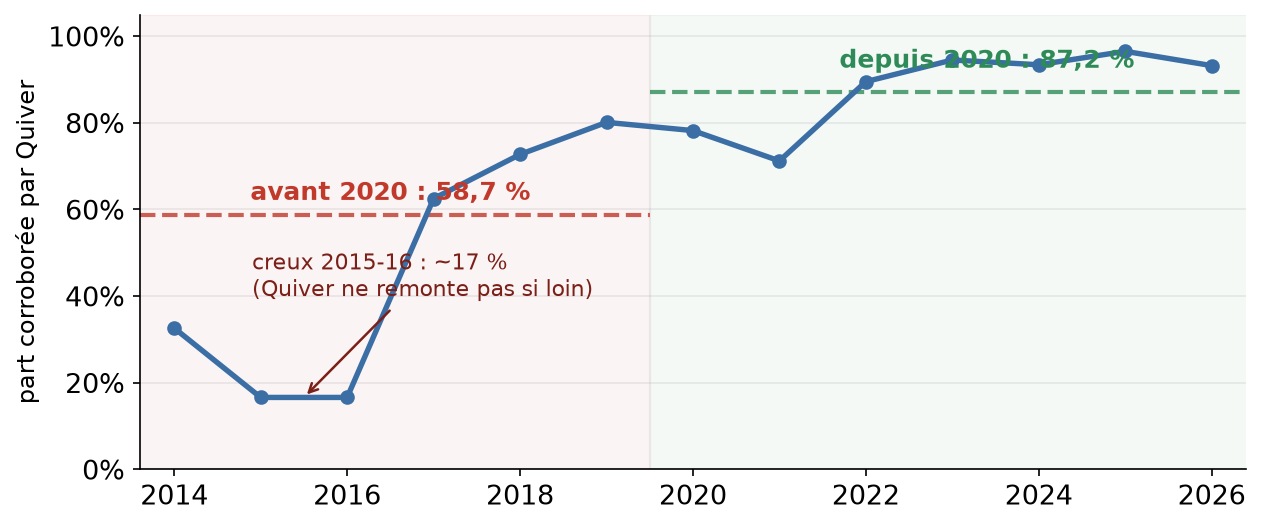
\includegraphics[width=\linewidth]{png/figs_deck/corroboration_par_annee.png}\\[0.5mm]
      {\scriptsize\color{black!60} part de \textbf{nos} actions (Chambre, \co{Stock})
       que Quiver possède aussi --- par année civile de dépôt}
    \end{column}
    \begin{column}{0.40\textwidth}\footnotesize
      {\scriptsize\color{black!60} l'\textbf{autre sens} que la slide précédente :
       elle mesurait « combien de Quiver \textbf{retrouve-t-on} ? » (\textbf{92\,\%}) ;
       \textbf{ici}, « combien de \textbf{nos} actions Quiver \textbf{confirme-t-il} ? »}\\[2mm]
      {le taux global \textbf{lisse} une forte hétérogénéité : \mbox{\textbf{58,7\,\%}}
       avant 2020, \mbox{\textbf{87,2\,\%}} depuis --- creux \textbf{2015-16} à
       $\sim$17\,\%.}\\[2mm]
      \colorbox{alertred!10}{\parbox{0.96\linewidth}{\scriptsize
        nos \textbf{15\,015} actions « en plus » d'avant 2020 portent des \textbf{tickers réels
        et d'époque} : ce n'est pas notre erreur, c'est \textbf{Quiver qui est mince avant
        $\sim$2017} --- \textbf{\textcolor{alertred}{à retenir pour le backtest}} : moins de
        vérité-terrain externe sur l'ancien.}}
    \end{column}
  \end{columns}
\end{frame}

% ── 9 · Les autres preuves (ferme l'étape 9) ──
\begin{frame}{9 · Les autres preuves --- deux collectes tierces confirment nos lignes}
  \centering
  \vspace{0.5mm}
  {\footnotesize deux collectes publiques \textbf{indépendantes} re-lisent les mêmes PTR officiels ---
   comparées \textbf{ligne à ligne} (déposant · ticker · sens · date, \emph{montant hors clé}) :}\\[3.5mm]
  \begin{columns}[T]
    \begin{column}{0.47\textwidth}
      \carte{selec}{\senat{} --- senate-stock-watcher}{sur \textbf{5\,524} transactions d'actions,
        \textbf{99,7\,\%} retrouvées chez nous \textbf{à la transaction près}}
    \end{column}\hfill
    \begin{column}{0.47\textwidth}
      \carte{helec}{\chambre{} --- house-stock-watcher}{sur \textbf{23\,437} transactions d'actions,
        \textbf{99,6\,\%} retrouvées chez nous \textbf{à la transaction près}}
    \end{column}
  \end{columns}
  \vspace{2.5mm}

  {\scriptsize\color{black!60} deux lectures indépendantes qui \textbf{convergent} $\rightarrow$ notre
   lecture est robuste ; le reliquat ($<$0,4\,\%) = tickers exotiques + fonds/ETF que notre pipeline filtre}\\[4mm]
  \repband{\textbf{dehors} : $>$\,99,6\,\% de nos lignes d'actions retrouvées par 2 collectes tierces ·
   \textbf{dedans} : \textbf{368} tables reproduites à l'\textbf{octet} · et \textbf{rien n'est réinjecté}.}
\end{frame}

\section{Partie II · Proposition : le backtest}
\partdivider{helec}{PARTIE II}{Proposition : le backtest}{les élus battent-ils le marché\,? --- ce qu'on voit, ce qu'on a essayé}

\begin{frame}{Le point de départ : la table construite en Partie I}
  \centering\vfill
  {\large On dispose de \textbf{118\,029 transactions} exploitables (ticker coté + prix fiable),\\[1mm] \textbf{372 membres}, sur \textbf{2014--2026}.}\\[5mm]
  {\footnotesize Ici on ne refait pas la donnée : on regarde \textbf{à quoi ressemblent ces portefeuilles},\\ et \textbf{ce qu'on observe} quand on essaie de les copier.}
  \vfill
\end{frame}

% ═════════════════════════ SECTION A ═════════════════════════
\chapdivider{Étape A}{À quoi ressemble la population}{qui sont ces gens, et comment tradent-ils ?}

\begin{frame}{La population de trades dans le temps}
  \centering
  
\includegraphics[width=0.97\textwidth,height=0.60\textheight,keepaspectratio]{png/figs_pop/P1_population_temps.png}\\[2mm]
  \defl{\textbf{à gauche} : le nombre de membres qui passent au moins un trade dans l'année (une centaine environ) — la population active monte jusqu'en 2020 puis reflue. \textbf{à droite} : achats (vert) vs ventes (rouge), un flux globalement équilibré.}\\[1mm]
  \kpi{helec}{118\,029}{trades exploitables sur 2014--2026}\hspace{10mm}%
  \kpi{dataC}{$\sim$110}{membres actifs par an (372 au total)}
\end{frame}

\begin{frame}{Une poignée de membres fait l'essentiel des trades}
  \centering
  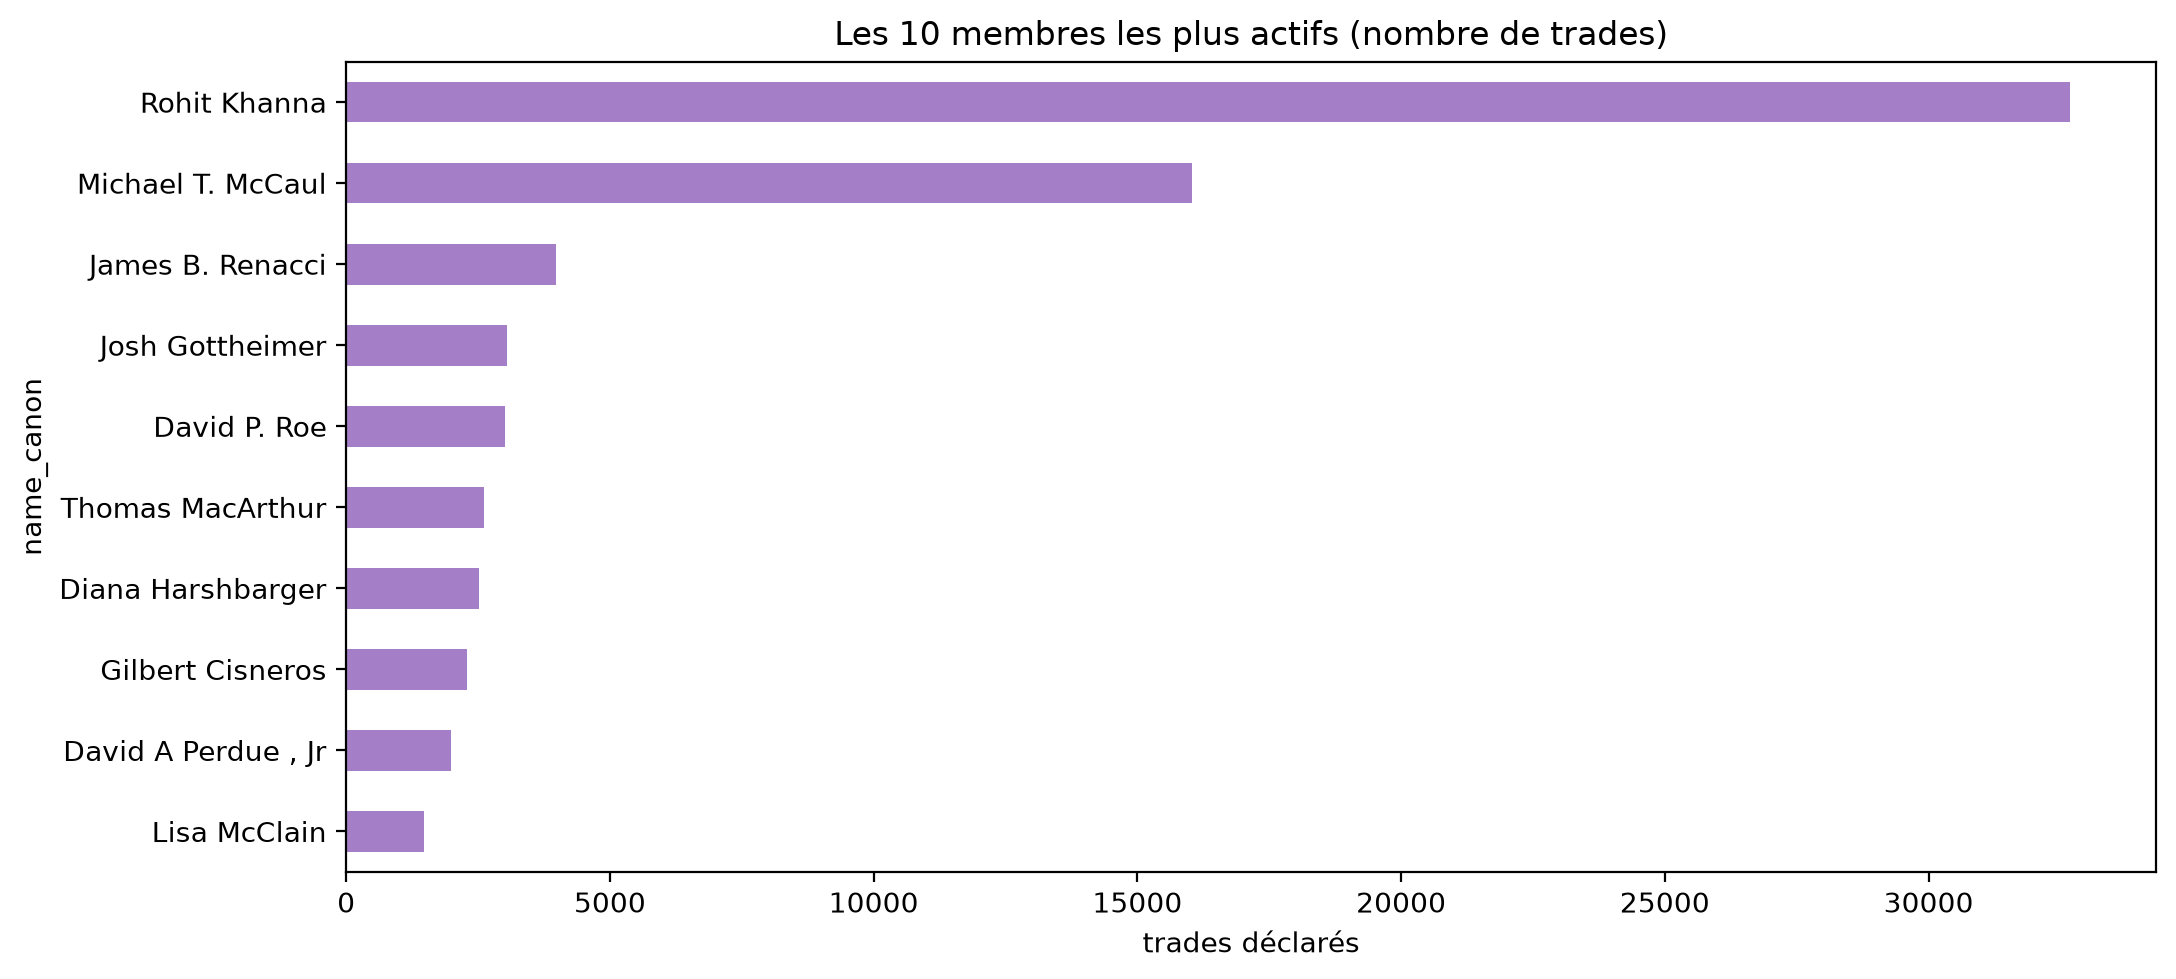
\includegraphics[width=0.9\textwidth,height=0.68\textheight,keepaspectratio]{png/figs_pop/P2_top_membres.png}\\[2.5mm]
  \kpi{alertred}{41\,\%}{des trades viennent des 2 plus actifs (Khanna, McCaul)}
\end{frame}

\begin{frame}{Les deux plus gros déposants ne tradent pas eux-mêmes}
  \centering
  {\footnotesize Le STOCK Act compte des \textbf{lignes déclarées} : chaque transaction \textgreater{}\,1\,000\,\$ du \emph{foyer} (élu, conjoint, enfants) = une ligne. Une fortune familiale en gestion déléguée en génère des milliers.}\\[1.5mm]
  \begin{tabular}{@{}l r r r@{}}
    \toprule
     & Khanna & McCaul & Pelosi (contraste)\\\midrule
    lignes déclarées & \textbf{35\,046} & \textbf{20\,296} & 141\\
    passées par l'élu lui-même & 2,3\,\% & 0,0\,\% & 28,4\,\%\\
    conjoint + enfants & 97,7\,\% & 100\,\% & 71,6\,\%\\
    tickers distincts & 1\,195 & 776 & 38\\
    taille médiane d'un trade & 8\,000\,\$ & 8\,000\,\$ & 375\,000\,\$\\
    rythme moyen & $\sim$3\,700/an & $\sim$1\,600/an & $\sim$12/an\\
    \bottomrule
  \end{tabular}\\[1.5mm]
  \kpi{alertred}{41,2\,\%}{de toutes les lignes viennent de ces 2 membres}\hspace{8mm}%
  \kpi{dataC}{100\,\%}{de leurs dépôts sont en papier scanné (OCR)}\\[1mm]
  \defl{fortunes familiales en trusts gérés par des professionnels (épouses héritières — Clear Channel côté McCaul) : le gérant rebalance un portefeuille très diversifié → des micro-lignes à la taille minimale. « Plus gros déposant » $\ne$ « plus gros trader ».}
\end{frame}

\begin{frame}{Et souvent, c'est le conjoint qui passe l'ordre}
  \centering
  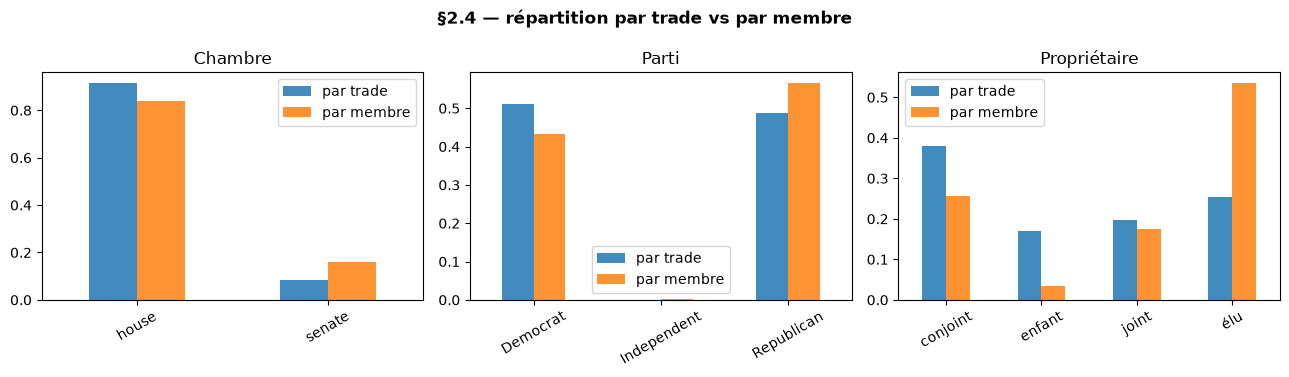
\includegraphics[width=0.95\textwidth,height=0.56\textheight,keepaspectratio]{png/figs_deck/A3_proprietaires.png}\\[2mm]
  \begin{tabular}{@{}l c c c c@{}}
    \toprule
    Propriétaire du compte & conjoint & élu & joint & enfant\\\midrule
    Part des trades & \textbf{37,9\,\%} & 25,4\,\% & 19,7\,\% & 17,0\,\%\\
    \bottomrule
  \end{tabular}\\[1.5mm]
  \defl{parts calculées sur \emph{l'ensemble des trades de tous les membres} (une moyenne de population, pas un membre en particulier) : le conjoint trade plus souvent que l'élu lui-même.}
\end{frame}

\begin{frame}{Les montants sont déclarés par fourchettes}
  {\small $\displaystyle a_j \;=\; \tfrac{1}{2}\bigl(\underline{m}_j+\overline{m}_j\bigr)$}\hspace{6mm}
  \defl{la loi ne déclare qu'un intervalle $[\underline{m}_j,\overline{m}_j]$ (STOCK Act) — on retient le milieu $a_j$ comme montant du trade $j$.}\\[1.5mm]
  \centering
  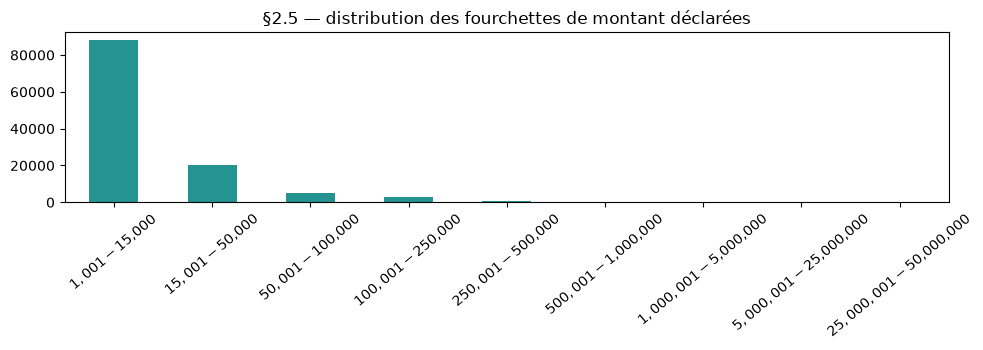
\includegraphics[width=0.95\textwidth,height=0.54\textheight,keepaspectratio]{png/figs_deck/A4_tailles.png}\\[2mm]
  \kpi{helec}{75\,\%}{des trades dans la 1\up{re} tranche (milieu 8\,000\,\$)}
\end{frame}

\begin{frame}{Ils déclarent en moyenne 27 jours après le trade}
  {\small $\displaystyle \mathrm{lag}_j \;=\; \delta_j-\tau_j \;\le\; 45\text{ j (délai légal)}$}\hspace{6mm}
  \defl{$\tau_j$ = date de la transaction (inaccessible en direct) ; $\delta_j$ = date de divulgation (la seule qu'un copieur voit).}\\[1.5mm]
  \centering
  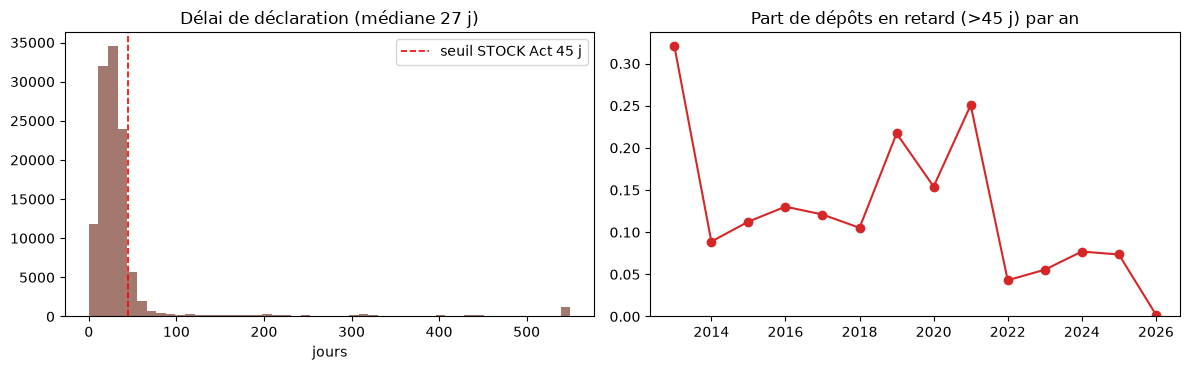
\includegraphics[width=0.95\textwidth,height=0.52\textheight,keepaspectratio]{png/figs_deck/A5_delai.png}\\[2mm]
  \kpi{helec}{27 j}{délai médian trade → divulgation}\hspace{10mm}%
  \kpi{warnorange}{11,7\,\%}{déclarations en retard ($>45$ j)}
\end{frame}

\begin{frame}{Achètent-ils dans les secteurs qu'ils régulent ?}
  \centering
  {\small $\displaystyle \text{align}_m \;=\; \frac{\#\{\text{achats de }m : \text{secteur}_{\text{GICS}}\in \text{juridiction de ses comités}\}}{\#\text{achats de }m}$}\\[1mm]
  \defl{chaque comité (via sa « jurisdiction » officielle) est relié à des secteurs GICS ; on regarde si le secteur du titre acheté en fait partie.}\\[2mm]
  
\includegraphics[width=0.97\textwidth,height=0.46\textheight,keepaspectratio]{png/figs_pop/P4c_conflit.png}\\[1.5mm]
  \kpi{helec}{16\,\%}{des achats tombent dans un secteur régulé par leurs comités}\hspace{5mm}%
  \kpi{warnorange}{quelques-uns}{très alignés (Hickenlooper $\sim$90\,\%)}\\[1mm]
  \repband{marché ultra-concentré (2 membres = 41\,\%), souvent via le conjoint (38\,\%), déclaré $\sim$27 j après ; alignement comité faible en moyenne (16\,\%).}
\end{frame}

% ═════════════════════════ SECTION B ═════════════════════════
\chapdivider{Étape B}{À quoi ressemble un portefeuille}{on ne déclare que des transactions ; on reconstruit le reste}

\begin{frame}{Un portefeuille se reconstruit trade par trade (FIFO)}
  \begin{columns}[T]
    \begin{column}{0.44\textwidth}
      \small
      \textbf{Achat} / \textbf{vente} du titre $i$, montant $a$ :\\[-4mm]
      \begin{align*}
        q &= \frac{a}{P_i(\tau)}\qquad\text{(achat)}\\
        q^- &= \min\!\Bigl(\tfrac{a}{P_i(\tau)},\, n_i(\tau^-)\Bigr)\quad\text{(vente)}
      \end{align*}
      \textbf{Positions et valeur} :\\[-4mm]
      \begin{align*}
        n_i(t) &= \textstyle\sum_{\text{achats}} q-\sum_{\text{ventes}} q^-\\
        V(t)   &= \textstyle\sum_i n_i(t)\,P_i(t)
      \end{align*}
      \defl{$\tau$ = 1\up{er} jour coté $\ge$ date du trade ; $P_i(t)$ = prix ajusté (dividendes, splits). $V(t)$ saute à chaque apport → figure.}
\end{column}
    \begin{column}{0.54\textwidth}\centering
      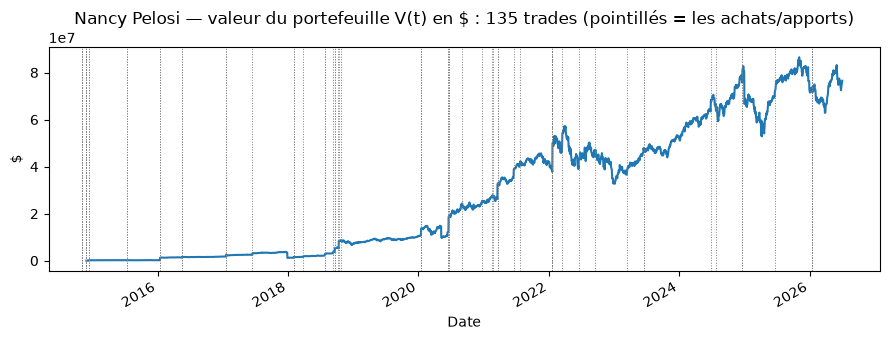
\includegraphics[width=\linewidth,height=0.72\textheight,keepaspectratio]{png/figs_deck/B1_vt_membre.png}
    \end{column}
  \end{columns}
\end{frame}

\begin{frame}{Le rendement « en parts » : un apport n'est jamais une performance}
  \begin{columns}[T]
    \begin{column}{0.44\textwidth}
      \small
      \textbf{Rendement time-weighted} (parts de la veille), puis \textbf{NAV} :\\[-4mm]
      \begin{align*}
        r_P(t) &= \frac{\sum_i n_i(t{-}1)\,P_i(t)}{\sum_i n_i(t{-}1)\,P_i(t{-}1)}-1\\
        \mathrm{NAV}(t) &= 100\textstyle\prod_{s\le t}\bigl(1+r_P(s)\bigr)
      \end{align*}
      \defl{\textbf{winsorisation} : on plafonne chaque rendement journalier à $\pm50\,\%$ — pour qu'un prix aberrant ou un saut ponctuel ne fausse pas la mesure.}\\[1.5mm]
      \begin{tabular}{@{}l r@{}}
        \toprule
        Les 266 portefeuilles & médiane\\\midrule
        CAGR & 12,8\,\%\\
        Volatilité & 21,6\,\%\\
        Sharpe & 0,71\\\bottomrule
      \end{tabular}
    \end{column}
    \begin{column}{0.54\textwidth}\centering
      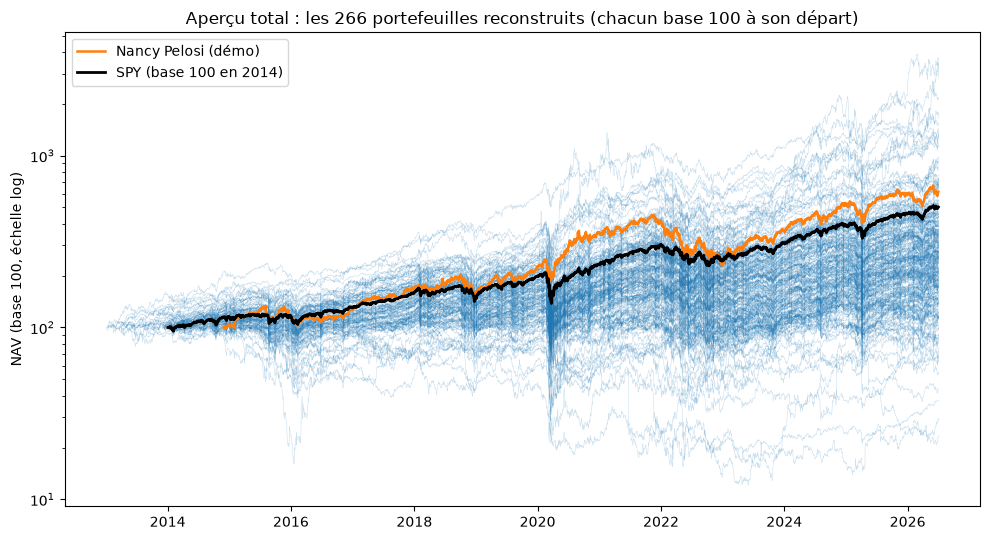
\includegraphics[width=\linewidth,height=0.64\textheight,keepaspectratio]{png/figs_deck/B2_spaghetti.png}
    \end{column}
  \end{columns}
\end{frame}

\begin{frame}{Ils gardent leurs positions longtemps}
  {\small $\displaystyle \text{durée}_i \;=\; \delta^{\text{vente}}_i - \delta^{\text{achat}}_i \quad(\text{appariement FIFO})$}\hspace{6mm}
  \defl{on apparie chaque vente au plus ancien achat non soldé (FIFO) ; la durée = l'écart entre les deux dates.}\\[1.5mm]
  \centering
  
\includegraphics[width=0.9\textwidth,height=0.56\textheight,keepaspectratio]{png/figs_pop/P5b_duree.png}\\[1.5mm]
  \kpi{helec}{$\sim$1 an}{avant de revendre (médiane 390 j)}\hspace{8mm}%
  \kpi{dataC}{44\,\%}{des positions ne sont jamais revendues}
\end{frame}

\begin{frame}{Chacun a ses secteurs de prédilection}
  \begin{columns}[T]
    \begin{column}{0.30\textwidth}
      \small Part du notional par secteur (heatmap membre $\times$ GICS, top-30 des membres).\\[3mm]
      \kpi{helec}{82}{membres à dominante informatique}\\[2mm]
      \kpi{dataC}{54}{membres à dominante finance}\\[2mm]
      \defl{la ligne = un membre ; la couleur = la part de ses achats dans le secteur.}
    \end{column}
    \begin{column}{0.68\textwidth}\centering
      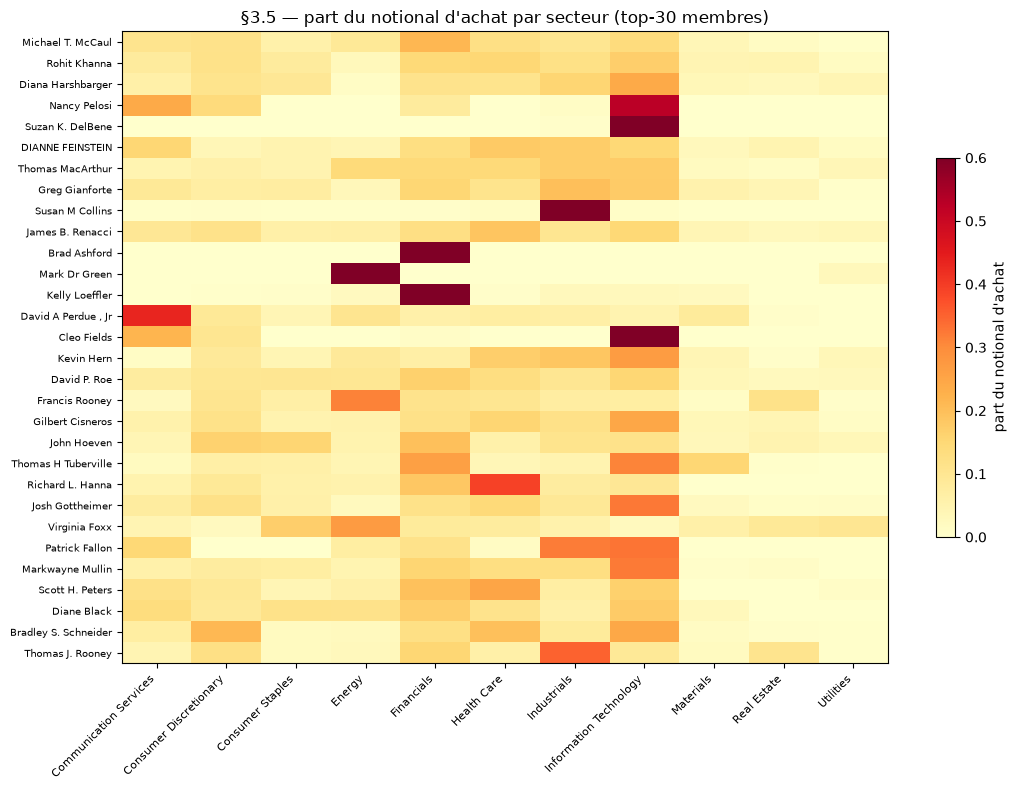
\includegraphics[width=\linewidth,height=0.70\textheight,keepaspectratio]{png/figs_deck/B6_secteurs.png}
    \end{column}
  \end{columns}
  \vspace{1mm}
  \repband{portefeuilles tenus longtemps ($\sim$1 an, 44\,\% jamais revendues), marqués par secteur.}
\end{frame}

% ═════════════════════════ SECTION C — LES STRATÉGIES ═════════════════════════
\chapdivider{Étape C}{Ce qu'on a essayé — une échelle de tests}{une seule question : peut-on gagner en copiant les mieux classés ?}

\begin{frame}{La question naïve : le Congrès bat-il le marché ?}
  \centering
  
\includegraphics[width=0.97\textwidth,height=0.58\textheight,keepaspectratio]{png/figs_pop/P7a_distributions.png}\\[2mm]
  \kpi{helec}{34\,\%}{des éligibles battent le SPY sur leur fenêtre}\hspace{8mm}%
  \kpi{dataC}{0,72 / 0,83}{Sharpe médian membres / SPY}
\end{frame}

% ── porte d'entrée (version V2) ──
\begin{frame}{La porte d'entrée : 223 membres sur 266 sont jugeables}
  \centering
  {\footnotesize éligible $\iff$ $n_{\text{trades}} \geq 10$ \textbf{et} $n_{\text{jours}} \geq 126$ ($\sim$ 6 mois de bourse)}\\[2mm]
  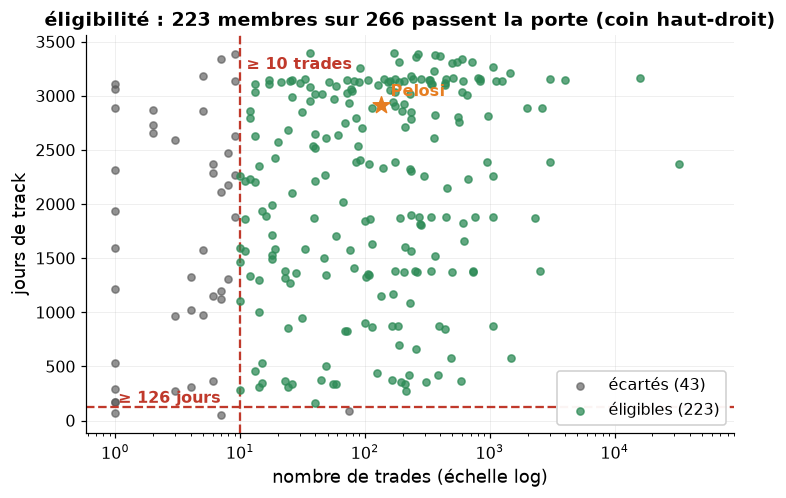
\includegraphics[height=0.62\textheight]{png/figs_deck/fig_05b_eligibilite.png}\\[1.5mm]
  \defl{sous les seuils : trop court pour distinguer chance et talent — \textbf{exclus du jugement}, pas des données.}
\end{frame}

% ── les deux mètres (version V2) ──
\begin{frame}{Deux mètres pour « battre le SPY » : l'écart brut (IR) ou l'alpha ajusté du $\beta$}
  \begin{columns}[T]
    \begin{column}{0.54\textwidth}
      {\color{helec}\footnotesize\textbf{Mètre 1 · IR — suppose $\beta = 1$}\; {\color{black!60}($x$ = excès quotidien / SPY)}}
      $$x(t)=r_P(t)-r_{\mathrm{SPY}}(t)\qquad \mathrm{IR}=\frac{\overline{x}}{\sigma(x)}\sqrt{252}$$
      \vspace{-2.5mm}
      {\color{dataC}\footnotesize\textbf{Mètre 2 · appraisal — estime $\beta$ (MCO), le retire}}
      $$r_P=\alpha+\beta\,r_{\mathrm{SPY}}+\varepsilon$$
      \vspace{-3.5mm}
      $$\beta=\frac{\mathrm{Cov}(r_P,r_{\mathrm{SPY}})}{\mathrm{Var}(r_{\mathrm{SPY}})}\qquad
        \mathrm{appr}=\frac{\alpha}{\sigma(\varepsilon)}\sqrt{252}$$
      \vspace{-2.5mm}
      {\color{black!70}\footnotesize\textbf{Le test}\; {\color{black!55}($n$ = jours de bourse du membre ; unilatéral)}}
      $$t_{\mathrm{IR}}=\mathrm{IR}\,\sqrt{\tfrac{n}{252}}\qquad
        t_{\mathrm{appr}}=\frac{\alpha}{\sigma(\varepsilon)}\sqrt{n}\qquad
        \text{seuil } t>1{,}645$$
      \centering
      \defl{$\beta=1 \ \Rightarrow\ $ appraisal $=$ IR}
    \end{column}
    \begin{column}{0.44\textwidth}\centering
      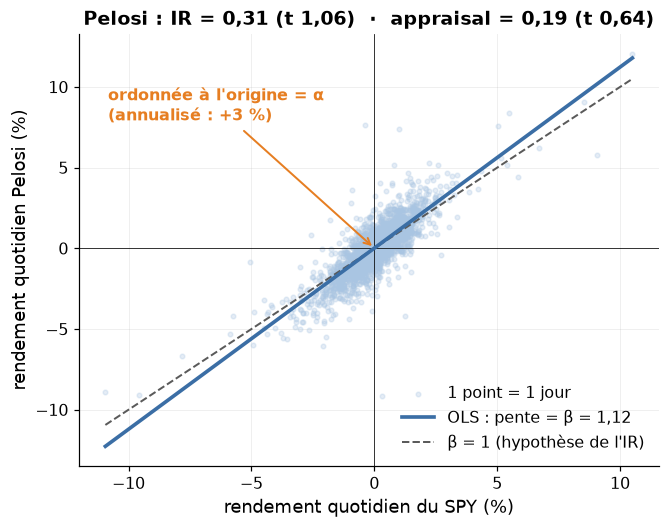
\includegraphics[width=0.93\linewidth]{png/figs_deck/fig_05b_regression_demo.png}\\[0.5mm]
      \defl{la pente absorbe le marché ; l'ordonnée à l'origine, c'est le talent.}
    \end{column}
  \end{columns}
\end{frame}

% ── la mesure : 20 -> 12 -> 11 (version V2, 2 histogrammes) ──
\begin{frame}{La mesure ne trouve presque rien : 20 « gagnants », 12 après le $\beta$, 11 par hasard}
  \centering
  \defl{diagnostic \textbf{rétrospectif} (\emph{in-sample}) : tout l'historique jugé d'un coup ($\approx$ 2014 → mi-2026), sur les \textbf{223 éligibles} — \emph{pas} encore de walk-forward.}\\[1.5mm]
  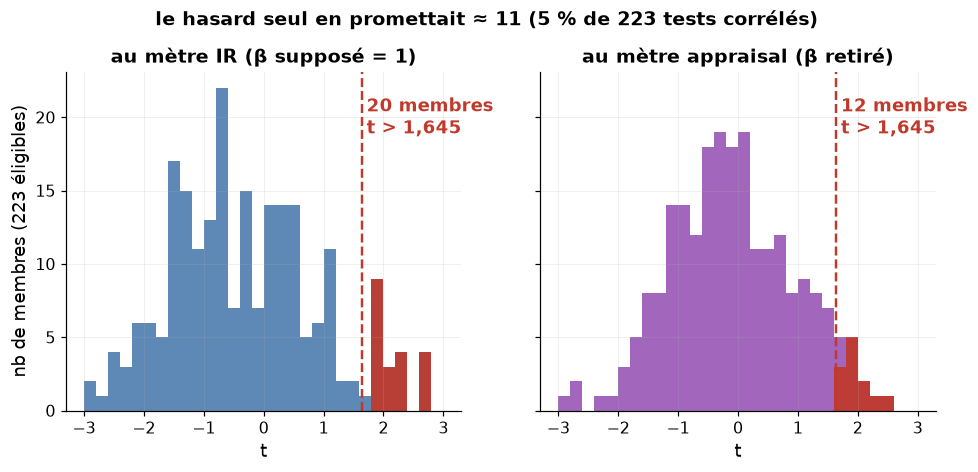
\includegraphics[height=0.54\textheight]{png/figs_deck/fig_05b_hist_t.png}\\[2mm]
  {\footnotesize \textbf{20} membres battent le SPY à l'IR, \textbf{12} seulement une fois le $\beta$ retiré (appraisal) — pour \textbf{$\approx$11} attendus par pur hasard (5 \% de 223).}
\end{frame}

% ── le tableau de sortie : les 20 (IR) et 12 (appraisal) + métriques ──
% ── tableau 1 : les 20 à l'IR ──
\begin{frame}{Les 20 « gagnants » à l'écart brut (IR)}
  \centering
  {\scriptsize
  \begin{columns}[T]
    \begin{column}{0.49\textwidth}\centering
      \begin{tabular}{@{}l r r r r r r@{}}
        \toprule
        Membre & $n$ & $\beta$ & IR & $t_{\mathrm{IR}}$ & appr & $t_{\mathrm{appr}}$\\\midrule
        Comstock & 85 & 1,20 & 0,90 & 2,77 & 0,66 & 2,03\\
        McGarvey & 24 & 1,53 & 1,50 & 2,76 & 1,08 & 1,99\\
        Suozzi & 662 & 1,22 & 0,90 & 2,68 & 0,59 & 1,75\\
        Fetterman & 10 & 1,17 & 2,48 & 2,64 & 2,24 & 2,38\\
        DelBene & 157 & 1,15 & 0,66 & 2,30 & 0,52 & 1,81\\
        Lawrence & 19 & 1,50 & 0,72 & 2,24 & 0,43 & 1,34\\
        Warner & 15 & 1,78 & 0,80 & 2,22 & 0,65 & 1,80\\
        Babin & 20 & 1,18 & 0,69 & 2,21 & 0,62 & 1,99\\
        Rouzer & 26 & 1,47 & 0,75 & 2,15 & 0,46 & 1,32\\
        Whitehouse & 718 & 1,04 & 0,57 & 2,07 & 0,51 & 1,85\\
        \bottomrule
      \end{tabular}
    \end{column}
    \begin{column}{0.49\textwidth}\centering
      \begin{tabular}{@{}l r r r r r r@{}}
        \toprule
        Membre & $n$ & $\beta$ & IR & $t_{\mathrm{IR}}$ & appr & $t_{\mathrm{appr}}$\\\midrule
        Moody & 23 & 1,79 & 1,67 & 2,01 & 1,36 & 1,64\\
        Kustoff & 10 & 1,44 & 0,79 & 1,99 & 0,54 & 1,37\\
        Gutierrez & 21 & 1,16 & 0,56 & 1,98 & 0,43 & 1,52\\
        Rooney & 597 & 1,14 & 0,56 & 1,94 & 0,48 & 1,67\\
        Wyden & 231 & 1,40 & 0,77 & 1,92 & 0,31 & 0,77\\
        McClain & 1\,479 & 1,76 & 1,26 & 1,92 & 0,83 & 1,27\\
        Evans & 173 & 1,08 & 0,61 & 1,89 & 0,47 & 1,46\\
        Sullivan & 100 & 1,57 & 1,00 & 1,89 & 0,43 & 0,82\\
        Roberts & 446 & 1,14 & 0,53 & 1,87 & 0,42 & 1,48\\
        Long & 49 & 1,24 & 0,57 & 1,82 & 0,29 & 0,94\\
        \bottomrule
      \end{tabular}
    \end{column}
  \end{columns}}\par\medskip
  \defl{les 223 éligibles → \textbf{20} passent le seuil à l'IR ($t_{\mathrm{IR}}>1{,}645$). Mais l'IR suppose $\beta=1$ ; en retirant le $\beta$, le classement change — \emph{tableau suivant}.}
\end{frame}

% ── tableau 2 : les 12 à l'appraisal (pas les mêmes membres) ──
\begin{frame}{Les 12 « gagnants » à l'alpha ajusté (appraisal) — pas les mêmes}
  \centering
  {\scriptsize $\dagger$ = absent des 20 de l'IR ($\beta$ faible : l'écart brut les sous-estimait)}\\[1mm]
  {\footnotesize
  \begin{tabular}{@{}l r r r r r r@{}}
    \toprule
    Membre & $n$ & $\beta$ & IR & $t_{\mathrm{IR}}$ & appr & $t_{\mathrm{appr}}$\\\midrule
    Ruiz\,$\dagger$ & 10 & 0,09 & $-$0,05 & $-$0,16 & 0,80 & 2,40\\
    Fetterman & 10 & 1,17 & 2,48 & 2,64 & 2,24 & 2,38\\
    Comstock & 85 & 1,20 & 0,90 & 2,77 & 0,66 & 2,03\\
    Sessions\,$\dagger$ & 361 & 0,93 & 0,31 & 1,15 & 0,55 & 2,01\\
    McGarvey & 24 & 1,53 & 1,50 & 2,76 & 1,08 & 1,99\\
    Babin & 20 & 1,18 & 0,69 & 2,21 & 0,62 & 1,99\\
    Hollingsworth\,$\dagger$ & 18 & 0,43 & 0,21 & 0,52 & 0,79 & 1,92\\
    Whitehouse & 718 & 1,04 & 0,57 & 2,07 & 0,51 & 1,85\\
    DelBene & 157 & 1,15 & 0,66 & 2,30 & 0,52 & 1,81\\
    Warner & 15 & 1,78 & 0,80 & 2,22 & 0,65 & 1,80\\
    Suozzi & 662 & 1,22 & 0,90 & 2,68 & 0,59 & 1,75\\
    Rooney & 597 & 1,14 & 0,56 & 1,94 & 0,48 & 1,67\\
    \bottomrule
  \end{tabular}}\\[2mm]
  \defl{\textbf{9} des 12 étaient déjà dans les 20 de l'IR ; \textbf{3} sont nouveaux ($\dagger$).}
\end{frame}

\begin{frame}{On va copier les mieux classés — cinq réglages à tester}
  \centering
  {\small On ne cherche pas à conclure : on \textbf{empile des tests}. Chaque test ne change \textbf{qu'un seul réglage} ; on monte d'un cran tant que l'excès \textbf{ne décroche pas} du marché (SPY).}\\[3mm]
  \resizebox{0.95\textwidth}{!}{%
  \begin{tikzpicture}
    \node[rung] (a) at (0,0)     {\textbf{Test 1}\\ QUI copier\\ {\scriptsize le top-4}};
    \node[rung] (b) at (3.3,0.7) {\textbf{Test 2}\\ COMBIEN\\ {\scriptsize le nombre $K$}};
    \node[rung] (c) at (6.6,1.4) {\textbf{Test 3}\\ QUAND\\ {\scriptsize la cadence}};
    \node[rung] (d) at (9.9,2.1) {\textbf{Test 4}\\ COMMENT\\ {\scriptsize les poids}};
    \node[rung] (e) at (13.2,2.8){\textbf{Test 5}\\ la RÈGLE\\ {\scriptsize le Sharpe}};
    \draw[-{Latex[length=2mm]},gray!70,line width=1pt] (a)--(b);
    \draw[-{Latex[length=2mm]},gray!70,line width=1pt] (b)--(c);
    \draw[-{Latex[length=2mm]},gray!70,line width=1pt] (c)--(d);
    \draw[-{Latex[length=2mm]},gray!70,line width=1pt] (d)--(e);
  \end{tikzpicture}}\\[3mm]
  {\footnotesize à chaque barreau : \textbf{la question · ce qu'on change · ce qu'on observe} — toujours face au même repère, le SPY.}
\end{frame}

% ── Test 1 · qui copier (walk-forward) ── [porté du deck données, fig_05b_*]
\begin{frame}{Test 1 · qui copier : le top-$K$, sans jamais regarder le futur}
  \begin{columns}[T]
    \begin{column}{0.51\textwidth}
      {\footnotesize \textbf{walk-forward} : à chaque coupe fin $Y$, on classe les éligibles
       ($t_{\text{crit}}>1{,}645$) et on tient le top-$K$ toute l'année $Y{+}1$ —
       \textbf{aucune info postérieure à la coupe}}\\[3.5mm]
      {\footnotesize \textbf{en parts} : chaque élu $k$ = un fonds de prix $\mathrm{NAV}^k$ ;
       à la coupe on \textbf{redéploie} le capital $W$ sur la nouvelle sélection, puis
       buy-and-hold jusqu'à la coupe suivante}\\[3.5mm]
      {\scriptsize\color{black!60} 11 coupes, fin 2015 → fin 2025 ; autofinancé (la NAV est
       continue) — \textbf{la mécanique en 3 temps, ci-après}}
    \end{column}
    \begin{column}{0.47\textwidth}\centering
      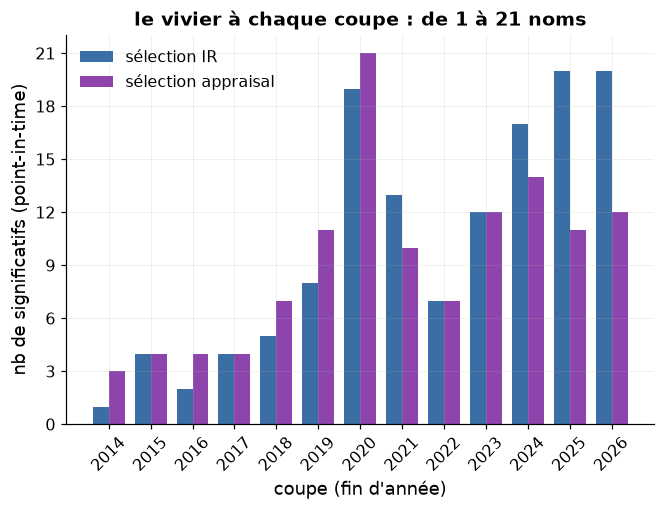
\includegraphics[width=\linewidth]{png/figs_deck/fig_05b_nsig_par_an.png}\\[1mm]
      {\scriptsize\color{black!60} le vivier à chaque coupe :
       de quoi alimenter un top-$K$ chaque année}
    \end{column}
  \end{columns}
\end{frame}

% ── Test 1 · le moteur en parts, en détail (3 temps) ──
\begin{frame}{Test 1 · le moteur en parts : compter, redéployer, tenir}
  \centering
  {\footnotesize membre $k$ = un fonds au prix de part $\mathrm{NAV}^k(t)=\prod_{s\le t}(1+r_k(s))$ ;
   on en détient $\mathrm{nbr}^k$ parts ; poids cibles $w_k=1/|S_Y|$ ; capital initial $W = 100$}\\[4mm]
  \resizebox{0.98\textwidth}{!}{%
  \begin{tikzpicture}[node distance=7mm]
    \node[step=grisC, text width=4.4cm] (n1)
      {\textbf{(i) COMPTER} à la coupe $t^R_Y$\\[1.5mm]
       $\displaystyle W=\!\!\sum_{k\in S_{Y-1}}\!\!\mathrm{nbr}^k_{Y-1}\,\mathrm{NAV}^k(t^R_Y)$};
    \node[step=helec, text width=4.0cm, right=of n1] (n2)
      {\textbf{(ii) REDÉPLOYER} sur la nouvelle sélection $S_Y$\\[1.5mm]
       $\displaystyle \mathrm{nbr}^k_Y=\frac{w_k\,W}{\mathrm{NAV}^k(t^R_Y)}$};
    \node[step=okgreen, text width=5.0cm, right=of n2] (n3)
      {\textbf{(iii) TENIR} (buy-and-hold, parts figées)\\[1.5mm]
       $\displaystyle \mathrm{NAV}(t)=\sum_{k\in S_Y}\mathrm{nbr}^k_Y\,\mathrm{NAV}^k(t)$\\[1mm]
       $\displaystyle r_{\text{strat}}(t)=\frac{\mathrm{NAV}(t)}{\mathrm{NAV}(t{-}1)}-1$};
    \draw[arr] (n1) -- (n2);
    \draw[arr] (n2) -- (n3);
    \draw[arr] (n3.south) .. controls +(0,-1.1) and +(0,-1.1) .. (n1.south)
      node[midway, below, font=\scriptsize\bfseries, gray] {coupe suivante};
  \end{tikzpicture}}\\[4mm]
  \badge{okgreen}{autofinancé — aucun apport, aucun retrait : la NAV est continue}\;
  \badge{warnorange}{entre deux coupes les poids DÉRIVENT (buy-and-hold, pas constant-mix)}
\end{frame}

% ── Test 1 · ce qu'on observe (top-4, 4 tuiles) ──
\begin{frame}{Test 1 · ce qu'on observe : +3,1 \%/an, mais porté par le $\beta$}
  \centering
  {\footnotesize\color{helec!85}\textbf{Test 1 · réglage de base} — $K=4$ fixe, équipondéré, annuel}\\[0.8mm]
  {\footnotesize 1 année civile = 1 observation :
   $x_Y=\prod_{t\in Y}(1+r_{\text{strat}})-\prod_{t\in Y}(1+r_{\mathrm{SPY}})$ ;\;
   $t=\overline{x}/\sigma(x)\cdot\sqrt{11}$ ; seuil $t_{10}\approx 1{,}81$}\\[1mm]
  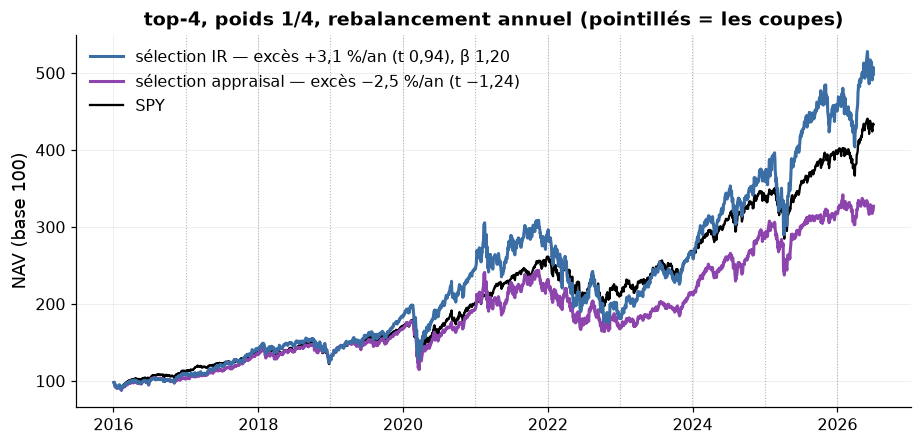
\includegraphics[height=0.40\textheight]{png/figs_deck/fig_05b_nav_top4.png}\\[2mm]
  \tuile{helec}{+3,1 \%/an}{excès brut\\7/11 années}\hfill
  \tuile{alertred}{t = 0,94}{sous le seuil\\1,81}\hfill
  \tuile{warnorange}{$\beta$ = 1,20}{l'excès = du style,\\pas du talent}\hfill
  \tuile{grisC}{$\alpha \approx 0$}{$t_{\text{appr}}$ −0,13 ;\\appraisal −2,5 \%/an}
\end{frame}

% ── Tests 2 & 3 · combien copier (K), et à quelle cadence ──
\begin{frame}{Tests 2 \& 3 · combien copier ($K$), et à quelle cadence}
  \centering
  {\footnotesize\color{helec!85}\textbf{Tests 2 \& 3} · on fait varier \textbf{COMBIEN} ($K$) et \textbf{QUAND} (cadence)}\\[0.8mm]
  {\footnotesize le top-4 ne passe pas → on laisse $K$ \textbf{s'ajuster chaque année}
   ($K^{*}(Y)=\arg\max_{K\in[4,20]}$ score sur le passé, walk-forward) et on rebalance tous les 6 mois}\\[1mm]
  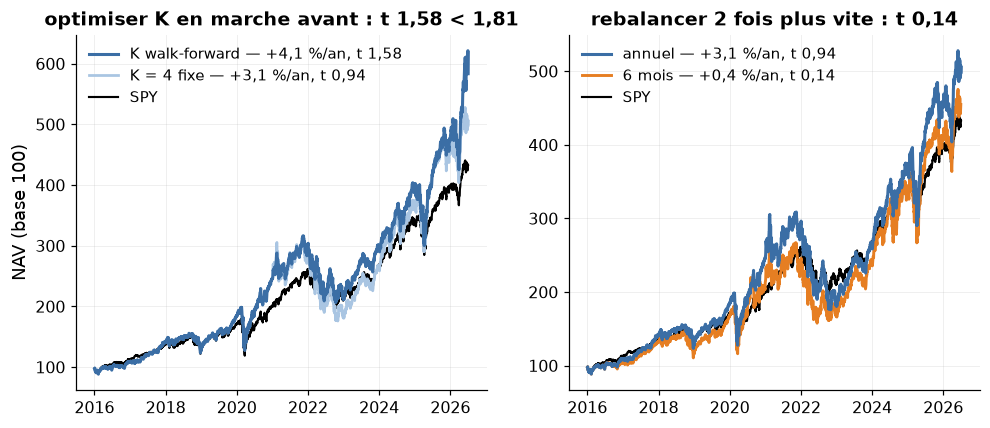
\includegraphics[width=0.55\textwidth]{png/figs_deck/fig_05b_k_et_cadence.png}\\[1.5mm]
  \badge{helec}{COMBIEN — $K$ walk-forward, annuel : +4,1 \%/an, t = 1,58}\\[1mm]
  \badge{warnorange}{QUAND — top-4 fixe, 6 mois : +0,4 \%/an, t = 0,14}\\[1.2mm]
  {\scriptsize\color{black!60} plus de liberté sur $K$ et la cadence — le $t$ monte un peu, ne passe jamais le seuil (1,81)}
\end{frame}

% ── Test 4 · comment répartir le capital ──
\begin{frame}{Test 4 · comment répartir le capital entre les copiés}
  {\footnotesize\color{black!80} jusqu'ici capital \textbf{à parts égales} ($1/K$). Mêmes membres (\textbf{top-4 fixe}) —
   on change seulement le \textbf{découpage du capital}, par le \textbf{risque}}
  {\scriptsize\color{black!55} (cadre : $w_k\ge 0$, $\textstyle\sum_k w_k=1$ ; $\Sigma_{ij}=\rho_{ij}\,\sigma_i\sigma_j$)}

  \vspace{1mm}
  \begin{columns}[T]
    \begin{column}{0.47\textwidth}
      {\footnotesize\color{helec}\textbf{inverse-vol}}\; {\scriptsize $\sigma_k=\mathrm{std}(r_k)\sqrt{252}$}
      $$w_k=\frac{1/\sigma_k}{\sum_j 1/\sigma_j}$$
      \vspace{-3mm}
      {\footnotesize\color{helec}\textbf{ERC}}\; {\scriptsize contributions au risque égales}
      $$w_k(\Sigma w)_k=w_j(\Sigma w)_j\ \ \forall\,k,j$$
      \vspace{-3mm}
      {\footnotesize\color{helec}\textbf{GMV}}\; {\scriptsize variance minimale, long-only}
      $$w^\star=\arg\!\min_{\sum w=1,\ w\ge 0}\ w^{\top}\Sigma w$$
      \vspace{-1mm}
      {\scriptsize\color{black!60} + $\Sigma$ stabilisée par shrinkage (Ledoit-Wolf) — annexe}
    \end{column}
    \begin{column}{0.51\textwidth}\centering
      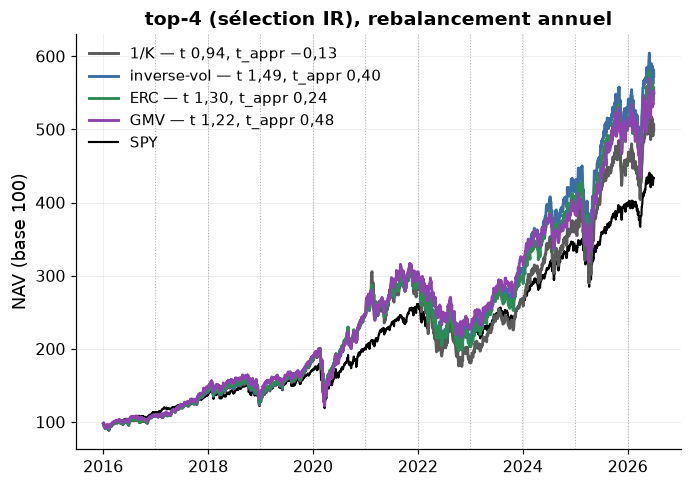
\includegraphics[width=0.92\linewidth]{png/figs_deck/fig_05b_ponderations.png}
    \end{column}
  \end{columns}
  \vspace{0.5mm}
  \centering
  {\scriptsize\color{black!60} GMV × sél. appraisal \textbf{sur-ajuste} (−4,5 \%/an) — \textbf{max $t_{\text{appr}} = +0{,}48$}, aucune ne fait apparaître d'$\alpha$}
\end{frame}

% ── Test 5 · changer la règle : le Sharpe brut ──
\begin{frame}{Test 5 · changer la règle de sélection : le Sharpe brut}
  \centering
  {\footnotesize\color{selec}\textbf{Test 5} · on change \textbf{QUI} (la règle de sélection) — les réglages restent les mêmes}\\[0.8mm]
  {\footnotesize $\mathrm{Sharpe}=\dfrac{\overline{r_P}}{\sigma(r_P)}\sqrt{252}$ ;\quad
   éligible v2 $\iff n_{\text{jours}}\ge 126$ \textbf{et} $\mathrm{Sharpe}>0{,}4$ — \textbf{plus aucun test t}}\\[1.5mm]
  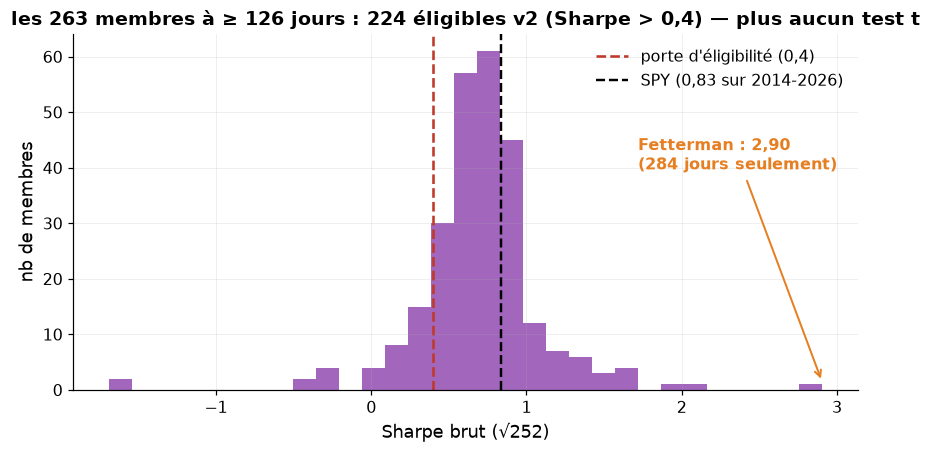
\includegraphics[height=0.48\textheight]{png/figs_deck/fig_05b_hist_sharpe.png}\\[1.5mm]
  {\footnotesize \textbf{224} éligibles (vs 223 en stratégie 1 — presque les mêmes) ;
   \textbf{même moteur} de copie en parts, seule la règle de classement change}\\[0.4mm]
  {\scriptsize\color{black!60} au prix d'admettre des historiques courts en tête (Fetterman 284 j, Sewell 4 trades)}
\end{frame}

% ── Test 5 · ce qu'on observe (balayage K) ──
\begin{frame}{Test 5 · ce qu'on observe : le $t$ plafonne à 1,22, loin du seuil}
  \centering
  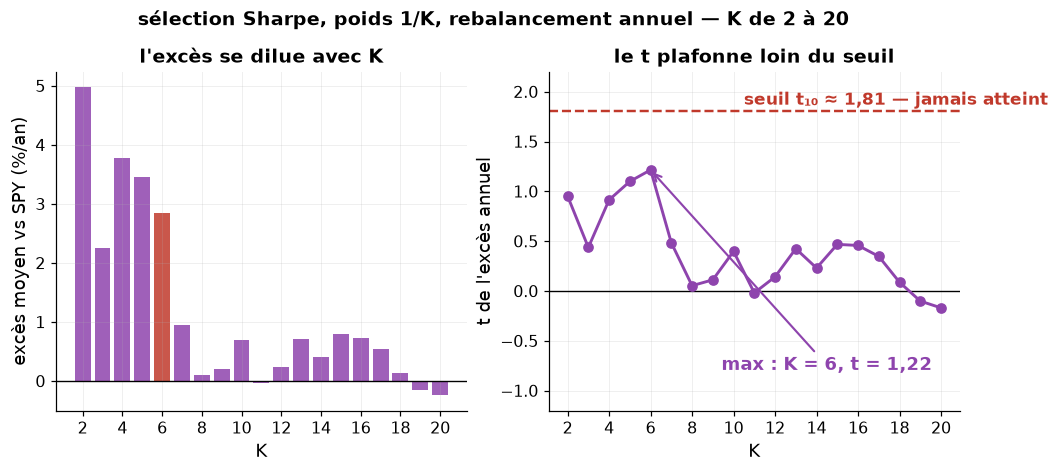
\includegraphics[width=0.62\textwidth]{png/figs_deck/fig_05b_balayage_k.png}\\[2mm]
  {\footnotesize balayage $K$ de 2 à 20 (poids $1/K$, annuel), plus 5 pondérations × 2 cadences
   ($K=5/10/20$) : le meilleur cas reste $K=6$, \textbf{$t=1{,}22$} ($<1{,}81$) ; l'excès se dilue quand $K$ grandit}\\[0.6mm]
  {\scriptsize\color{black!60} Sharpe 0,93 vs SPY 0,87 (fenêtre de tenue) — changer la règle ne fait pas non plus
   décrocher l'excès du marché}
\end{frame}

% ── grille récap : les 5 tests, sans verdict ──
\begin{frame}{Le bilan : cinq réglages testés, une même mesure}
  \centering
  {\footnotesize on lit \emph{ce qu'on change} et \emph{ce qu'on observe} (excès vs SPY, en $t$) — pas une sentence, une trace.}\\[2.5mm]
  {\footnotesize
  \begin{tabular}{@{}c l l l@{}}
    \toprule
     & On teste… & Ce qu'on change & Ce qu'on observe\\\midrule
    1 & copier le top-4 & --- (walk-forward, en parts) & $+3{,}1\,\%$/an, $\beta$ 1,20, t 0,94\\
    2 & combien copier & le nombre $K$ & meilleur cas t 1,58\\
    3 & quand rebalancer & la cadence (6 mois) & t 0,14\\
    4 & comment répartir & les poids (vol / corrélations) & rien ne décroche\\
    5 & qui mettre en tête & la règle (Sharpe brut) & t plafonne à 1,22\\
    \bottomrule
  \end{tabular}}\\[3mm]
  \kpi{grisC}{aucun}{réglage ne fait décrocher l'excès du marché}\hspace{7mm}%
  \kpi{helec}{un protocole}{de test réutilisable, prêt pour la suite}\\[2.5mm]
  {\footnotesize\color{black!60}\textbf{Ce qui reste à tester} : l'analyse par \emph{ticker} (le titre, pas la personne) · le \emph{drift court} juste après la divulgation.}
\end{frame}

% ═════════════════════════ SECTION D — LES PORTRAITS ═════════════════════════
\begin{frame}[plain]
  \centering\vfill
  {\color{helec!85}\large\textbf{Étape D}}\\[3mm]
  {\color{black!88}\fontsize{27}{31}\selectfont\textbf{Les portraits}}\\[3.5mm]
  {\color{helec!45}\rule{0.30\textwidth}{1.2pt}}\\[3.5mm]
  {\color{black!55}\large le classement a un « top » — qui sont ces membres, vraiment ?}\\[6mm]
  {\footnotesize\color{black!60} Chaque portrait suit le \textbf{même gabarit} : \textbf{(A)} NAV vs SPY (log) + drawdown · \textbf{(B)} trades (vert achat / rouge vente) · \textbf{(C)} poids des 8 positions · \textbf{(D)} excès annuel — et \textbf{toutes les stats en titre}.}
  \vfill
\end{frame}

\begin{frame}{Nancy Pelosi — $+3{,}4\,\%$/an vs SPY, mais non significatif ($\alpha$ t 0,64)}
  \centering
  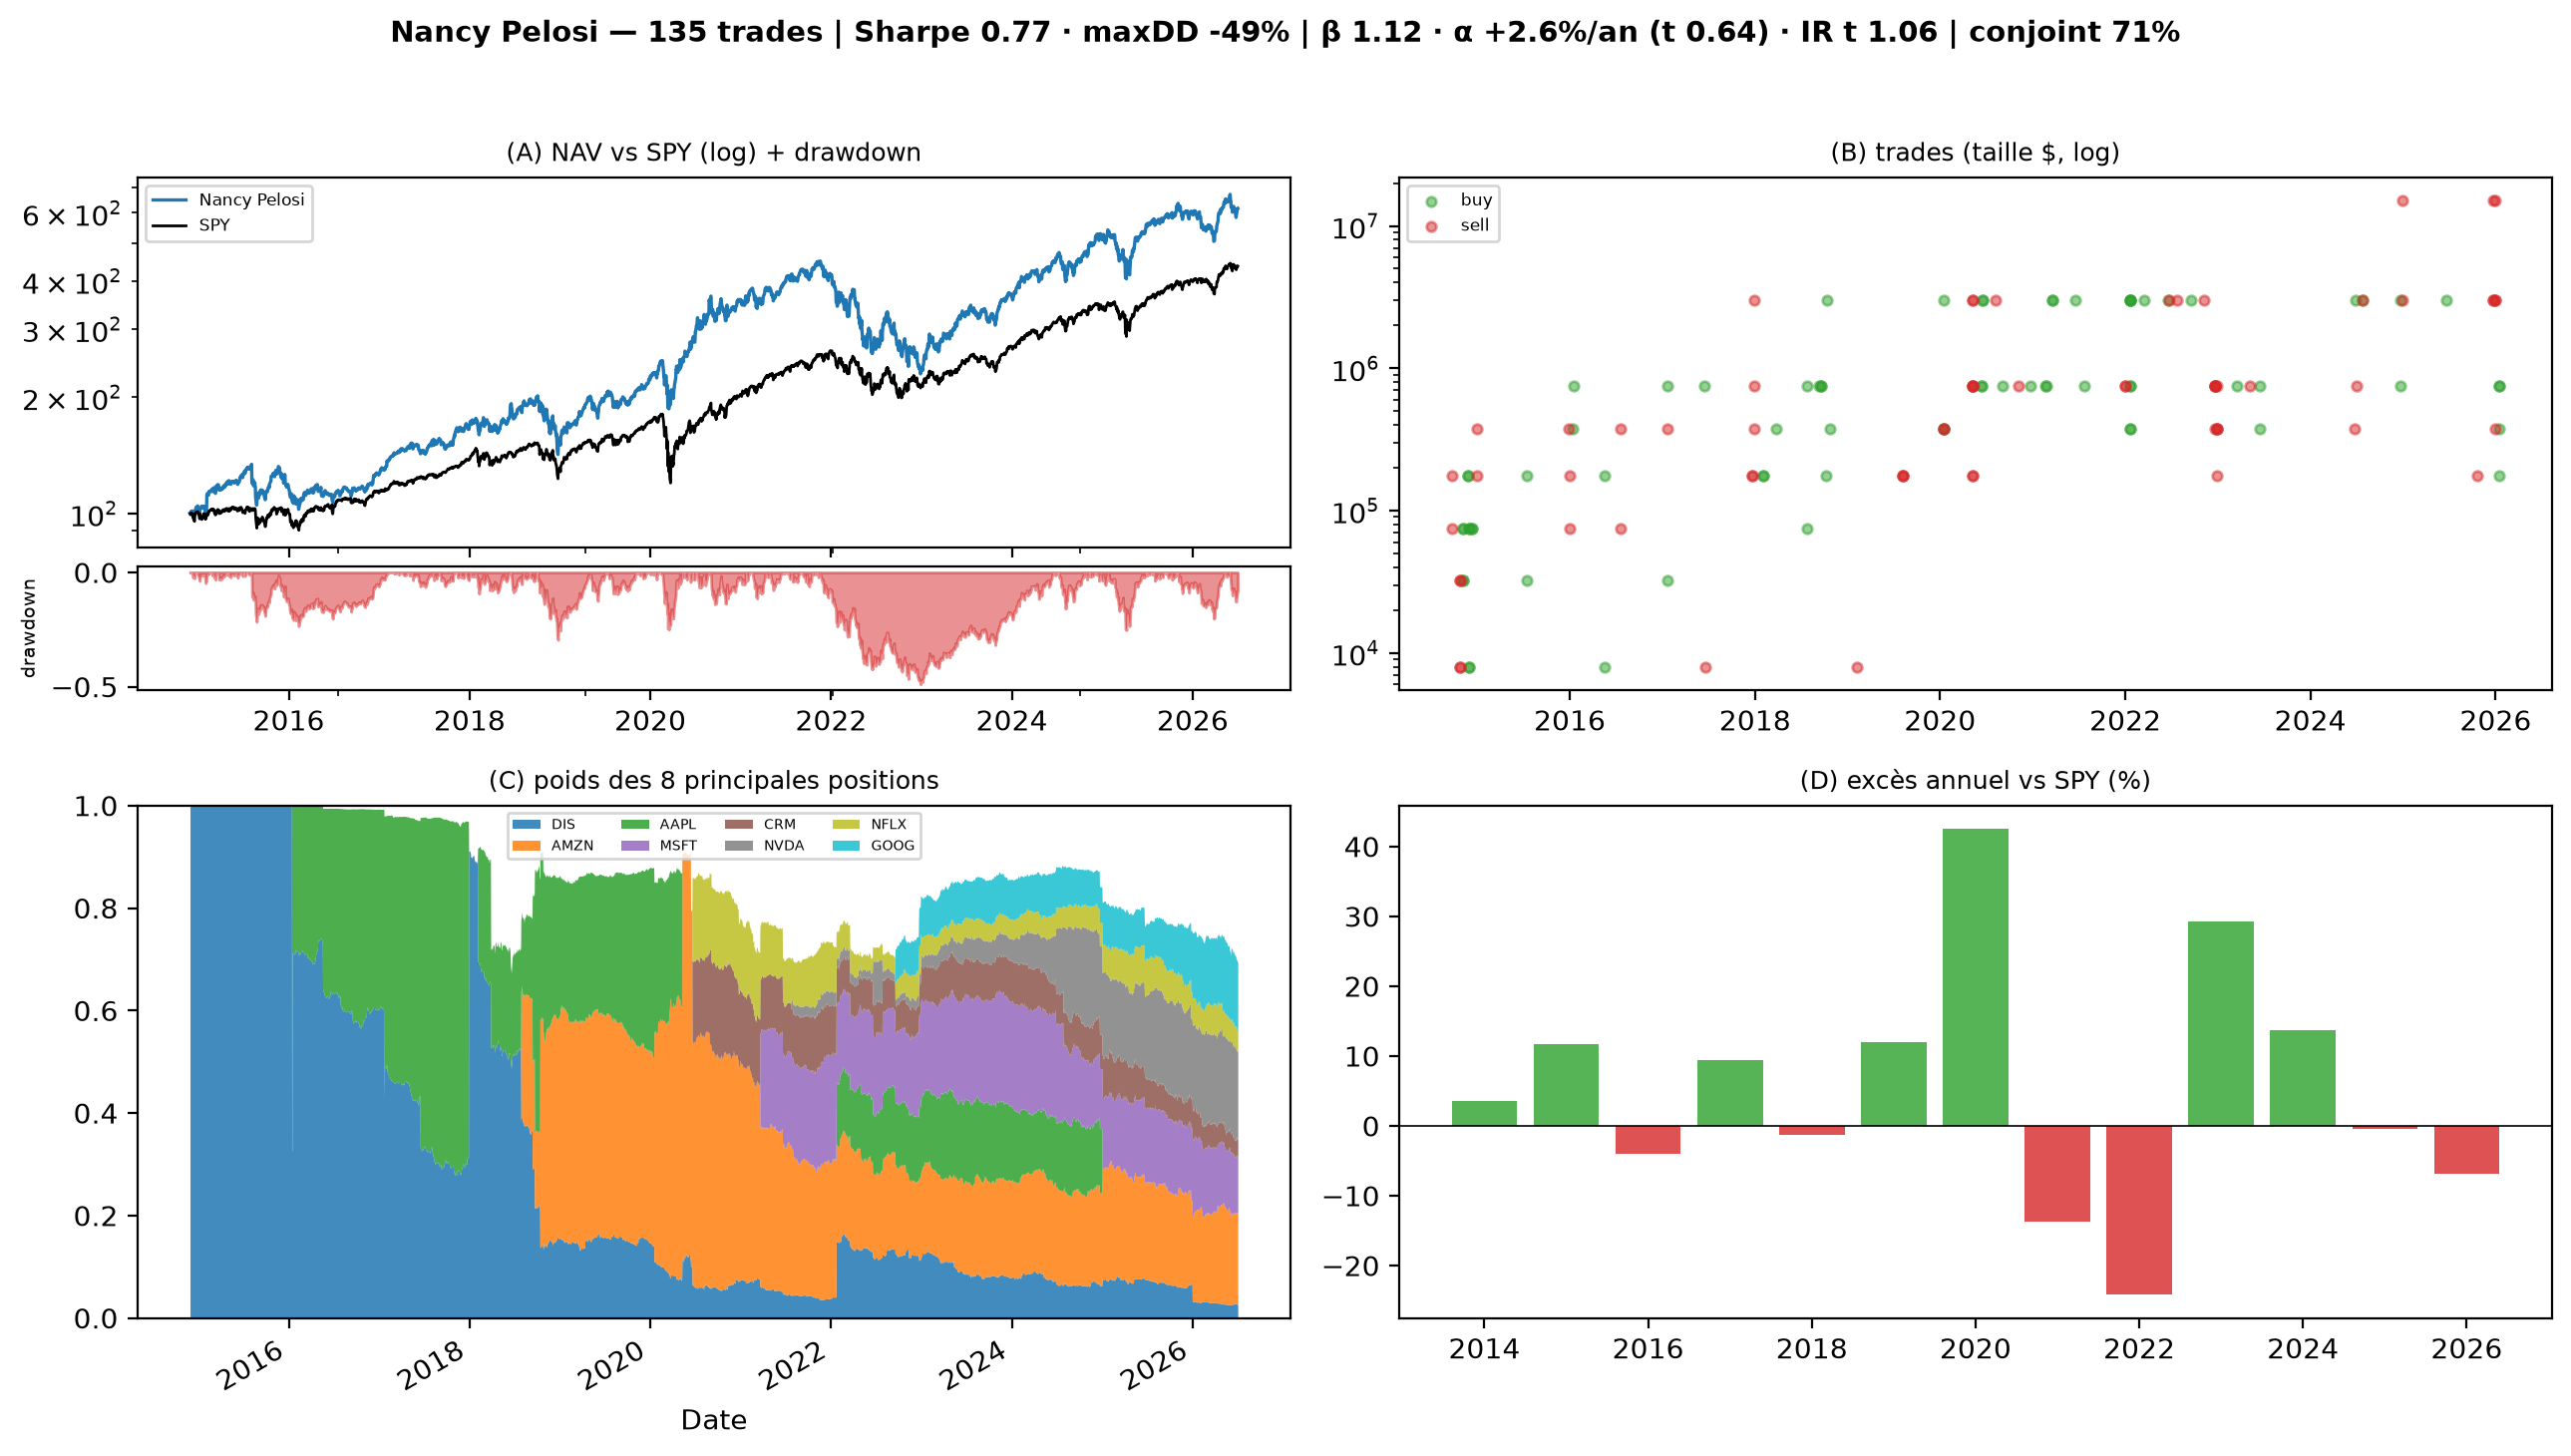
\includegraphics[width=0.98\textwidth,height=0.72\textheight,keepaspectratio]{png/figs_pop/G_P000197_portrait.png}\\[1mm]
  \kpi{helec}{$+3{,}4\,\%$/an}{de croissance au-dessus du SPY}\hspace{8mm}%
  \kpi{warnorange}{$\alpha$ t 0,64 · IR t 1,06}{indiscernable de la chance}
\end{frame}

\begin{frame}{Ro Khanna — 32\,700 trades, aucun avantage au niveau du trade (PF 0,88)}
  \centering
  
\includegraphics[width=0.98\textwidth,height=0.74\textheight,keepaspectratio]{png/figs_pop/G_K000389_portrait.png}\\[1mm]
  \kpi{helec}{$\sim$32\,700 trades}{Sharpe 0,87}\hspace{10mm}%
  \kpi{alertred}{PF 0,88 · IR t 0,13}{au niveau du trade, il perd contre le marché}
\end{frame}

\begin{frame}{John Fetterman — premier du classement, mais sur 10 trades et 1 an}
  \centering
  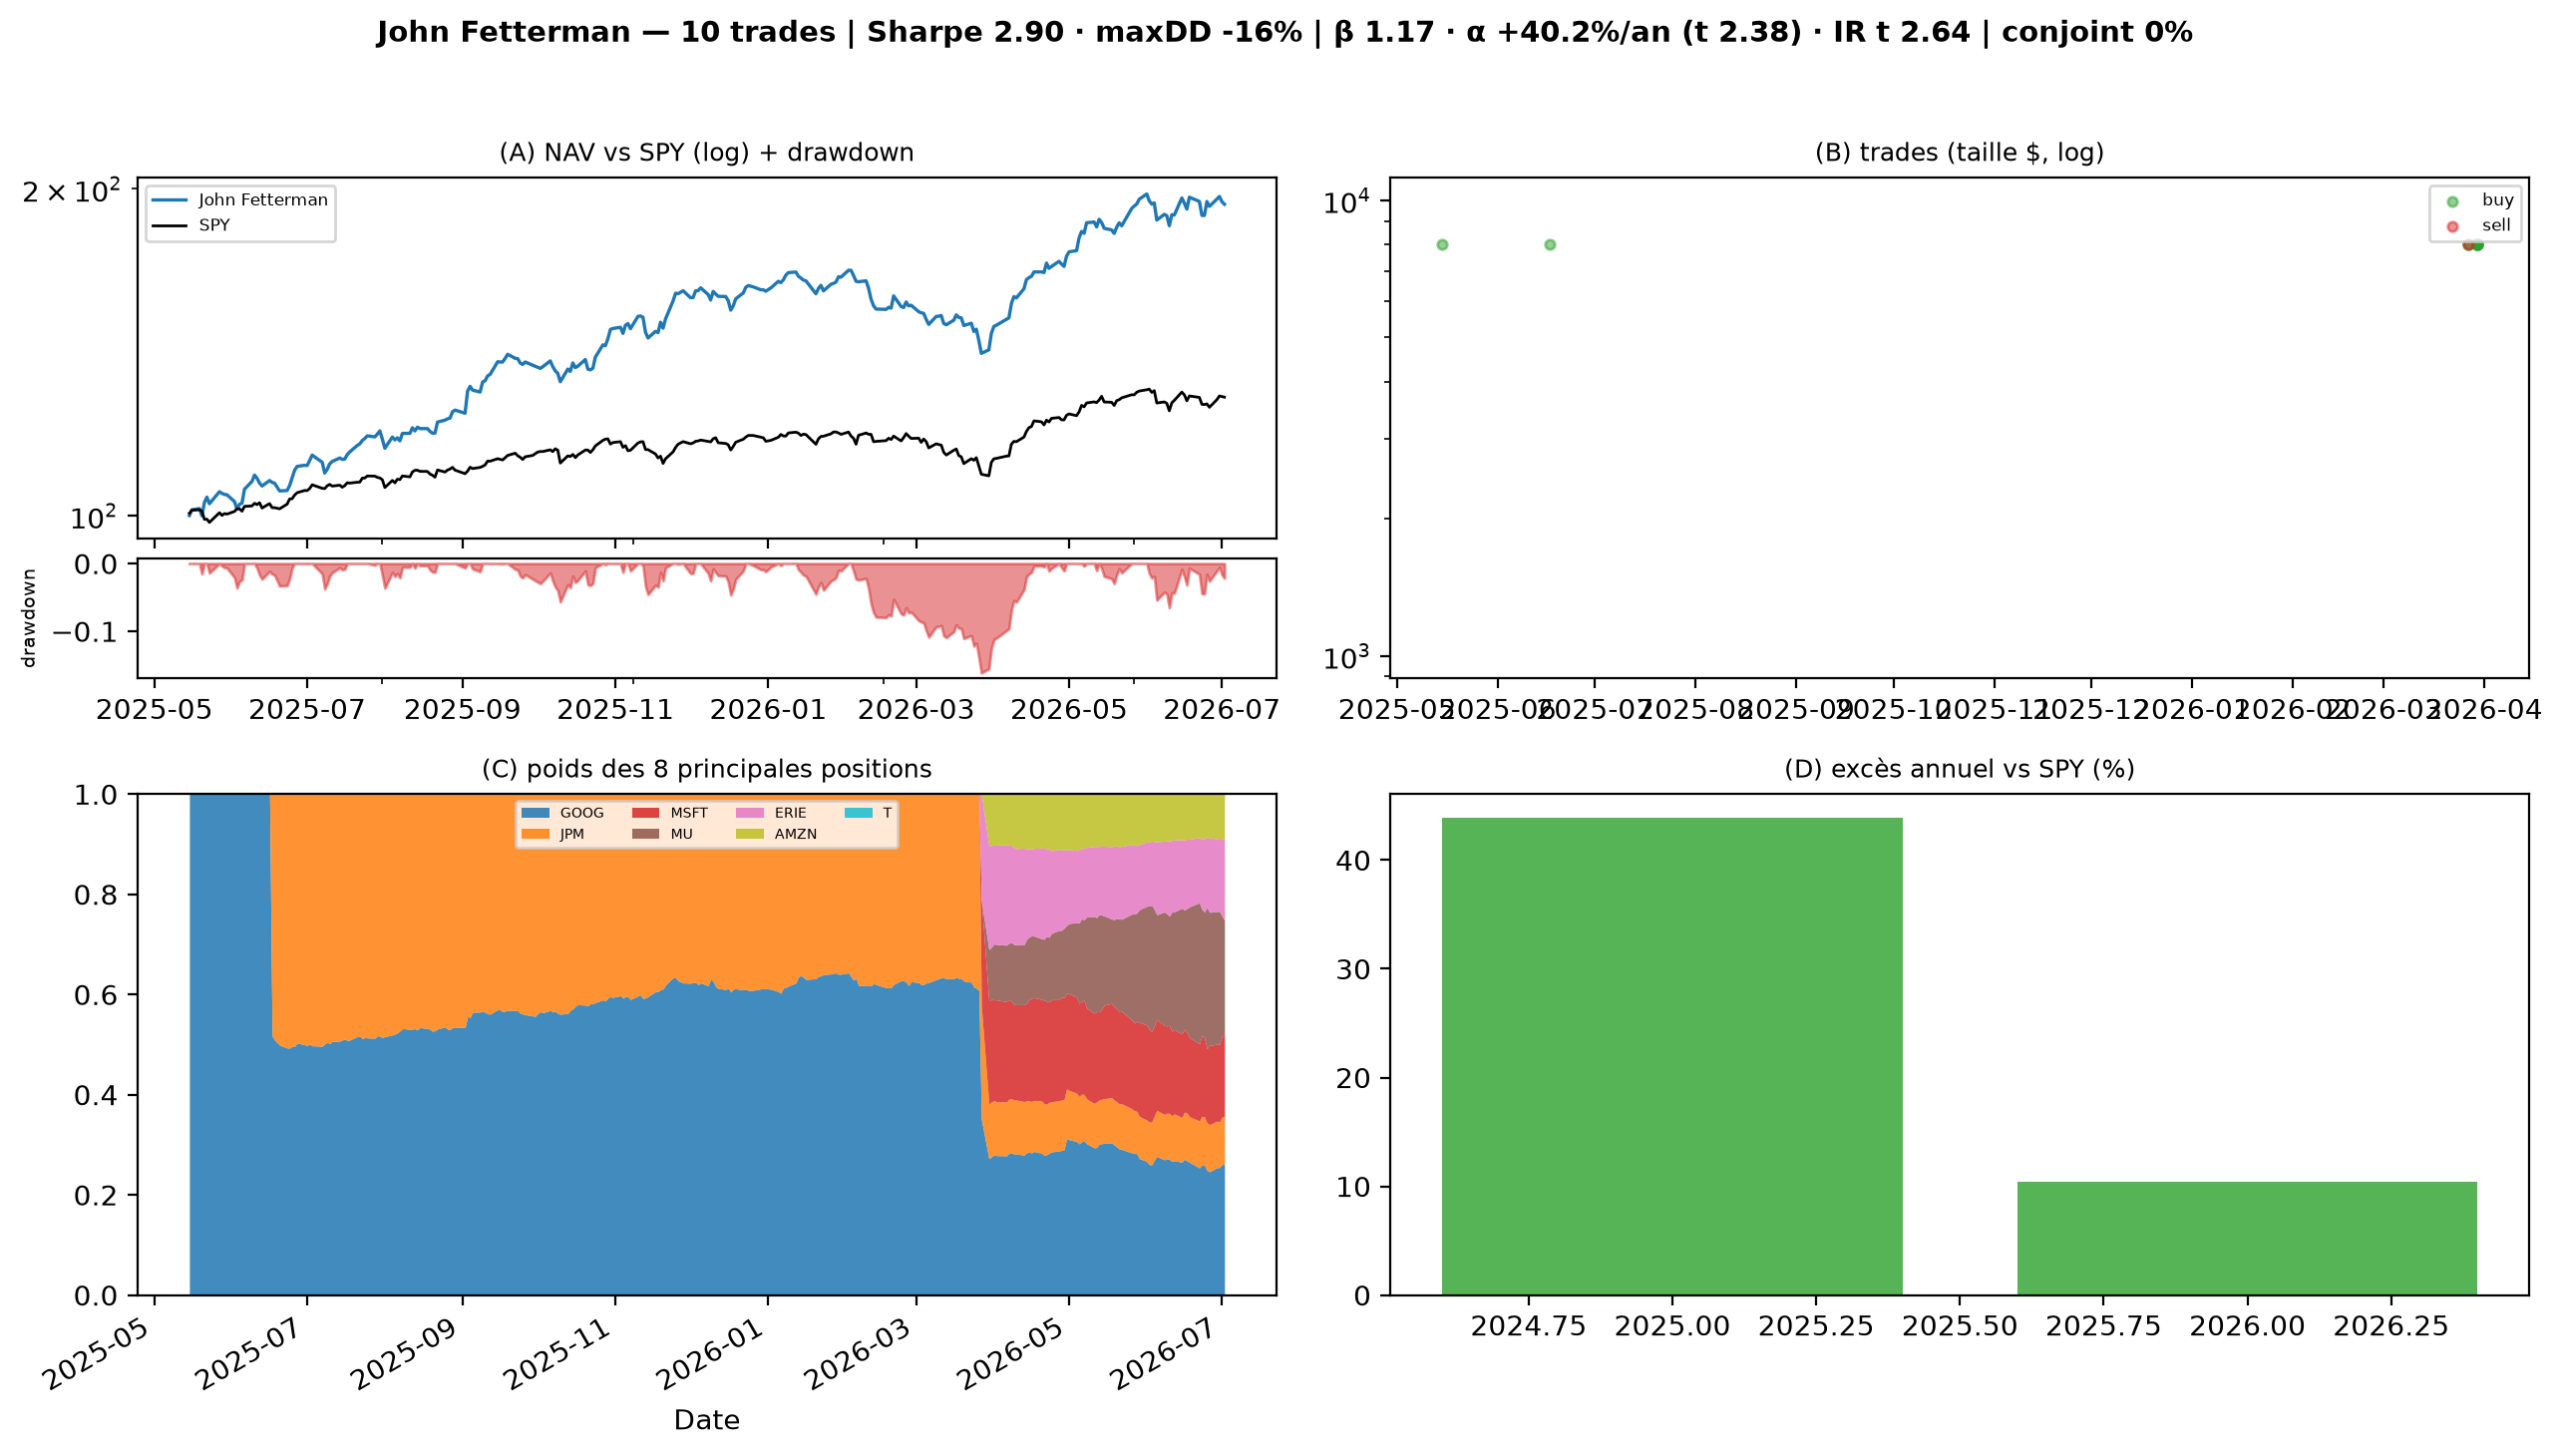
\includegraphics[width=0.98\textwidth,height=0.74\textheight,keepaspectratio]{png/figs_pop/G_F000479_portrait.png}\\[1mm]
  \kpi{okgreen}{Sharpe 2,90}{le plus haut du Congrès, en tête des 3 mètres}\hspace{6mm}%
  \kpi{alertred}{10 trades · 1 an}{l'outlier de queue — rien de reproductible}
\end{frame}

\begin{frame}{Sheldon Whitehouse — significatif sur 718 trades (le plus robuste), pour $+6\,\%$/an}
  \centering
  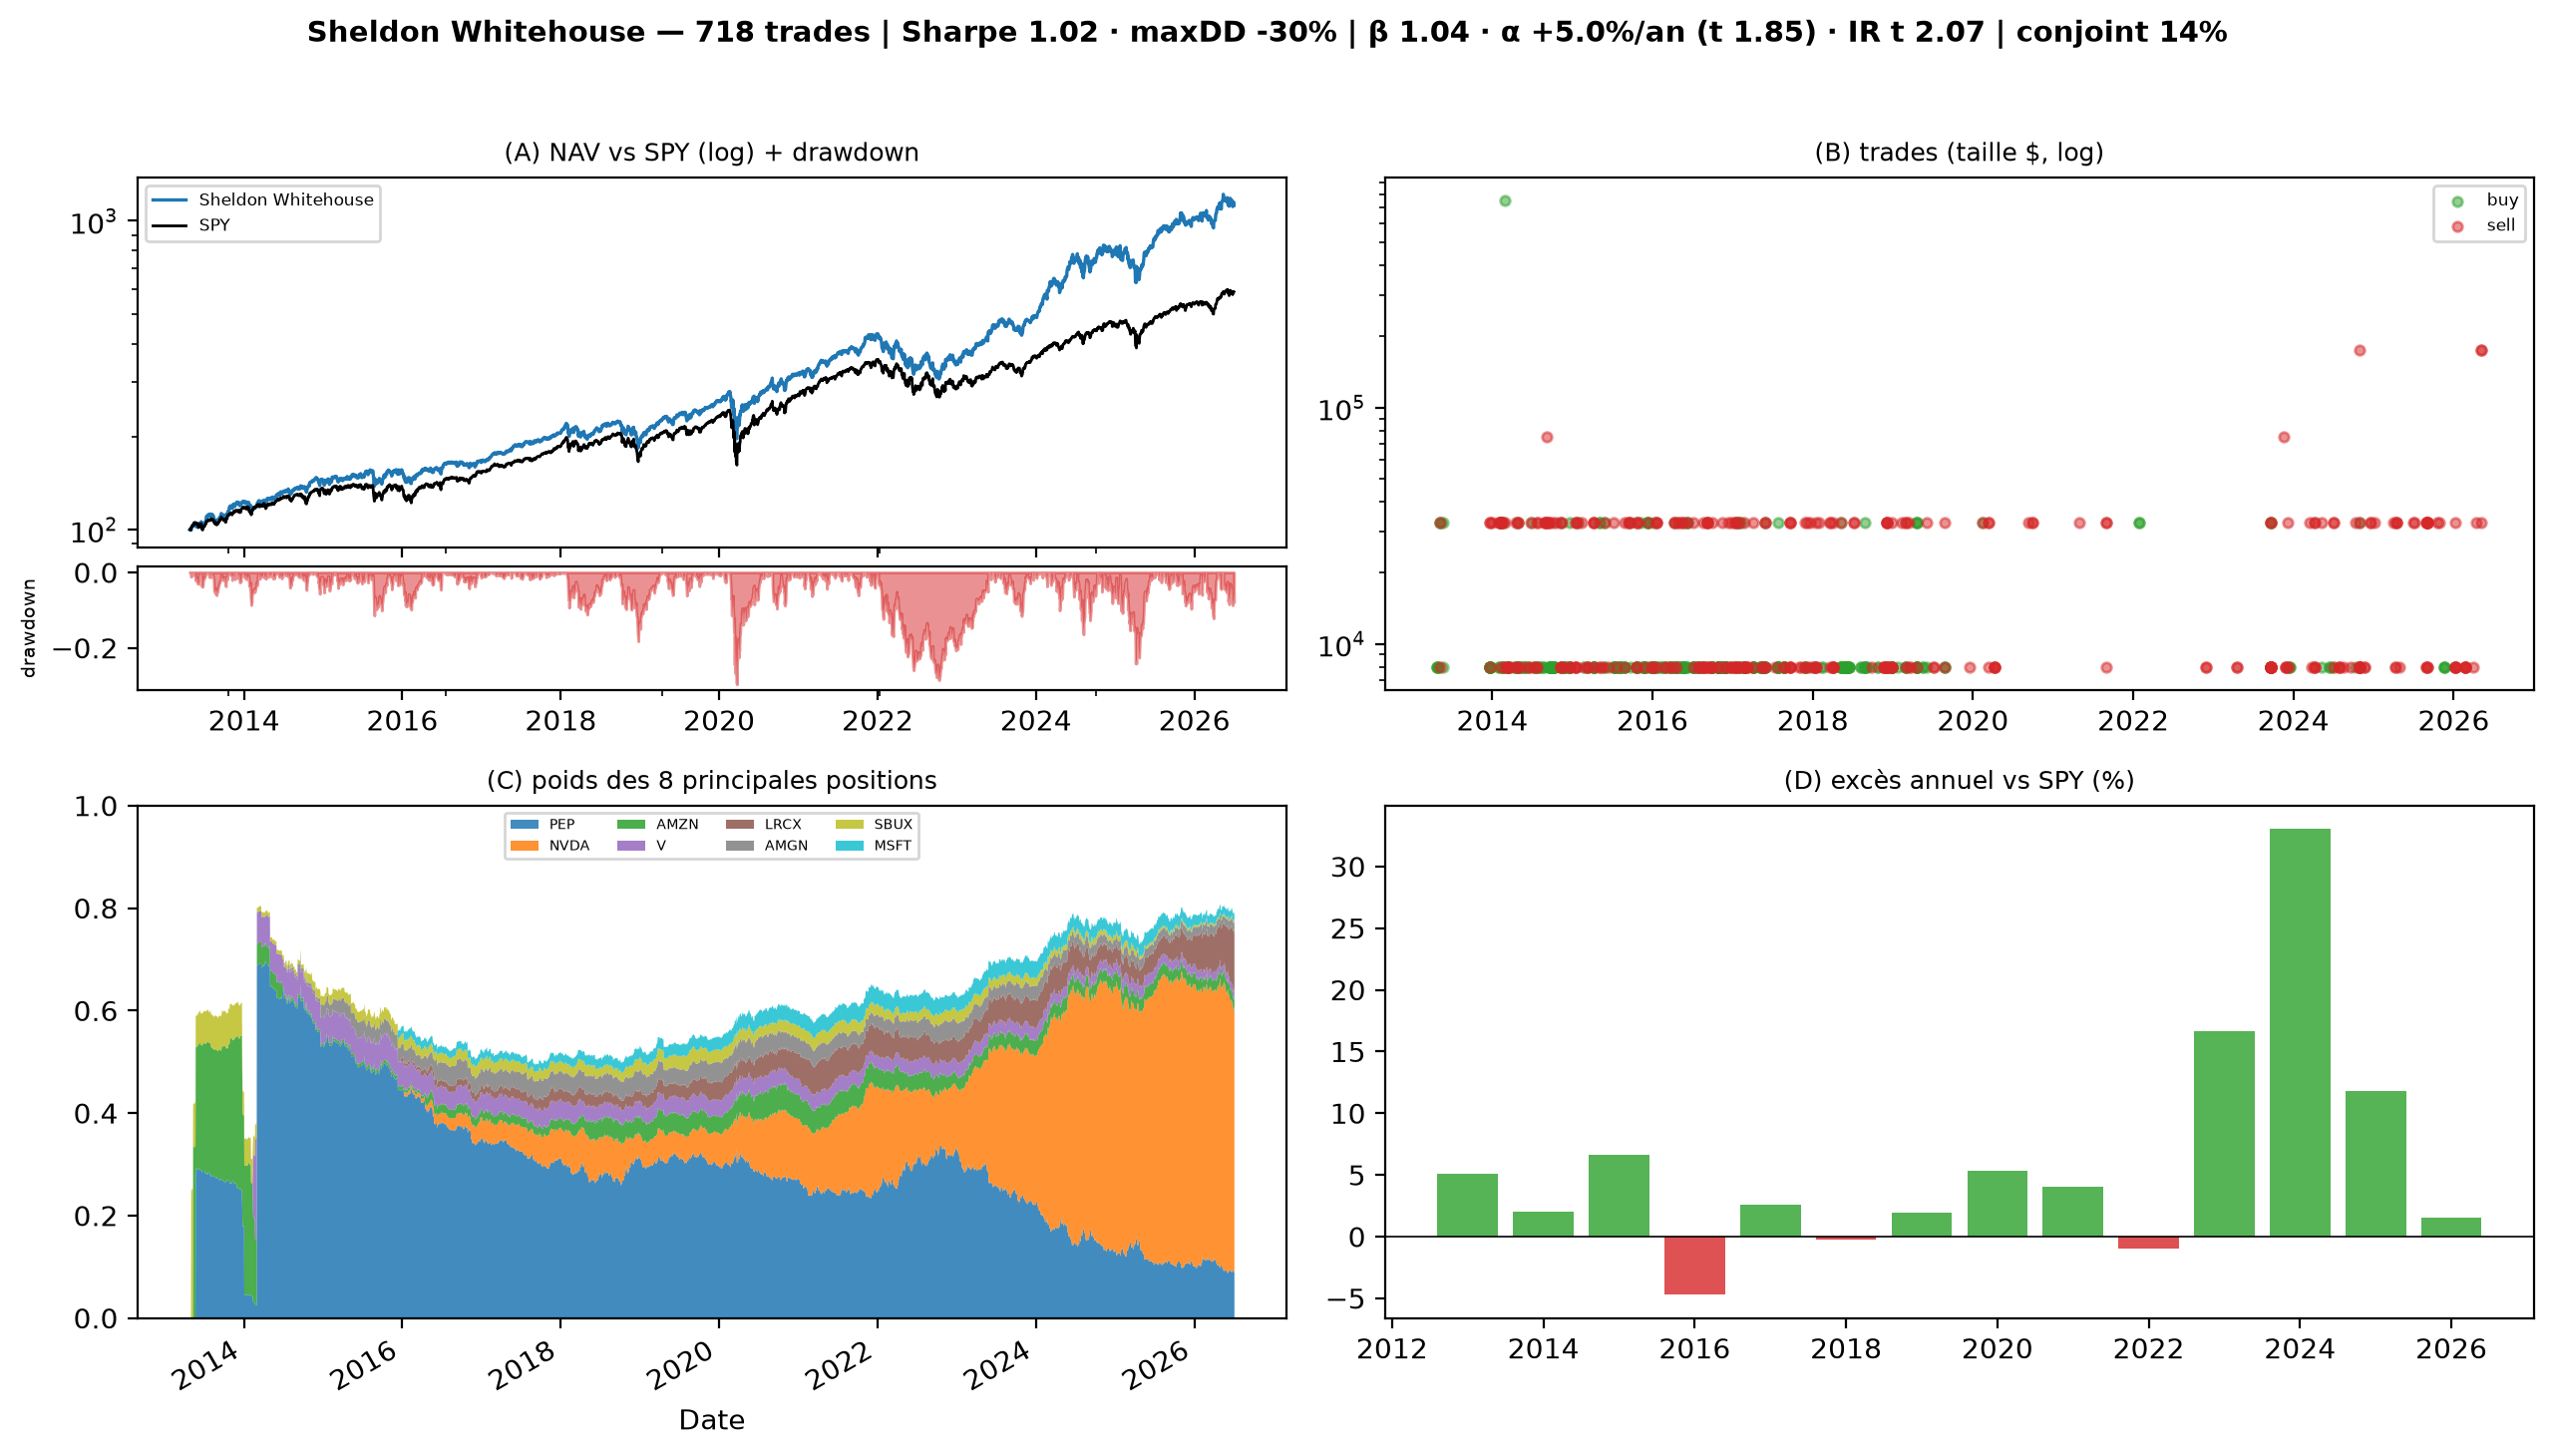
\includegraphics[width=0.98\textwidth,height=0.74\textheight,keepaspectratio]{png/figs_pop/G_W000802_portrait.png}\\[1mm]
  \kpi{helec}{IR t 2,07 · appr t 1,85}{significatif aux deux mètres, sur 718 trades}\hspace{6mm}%
  \kpi{dataC}{$+6\,\%$/an}{le candidat le plus sérieux — et pourtant modeste}
\end{frame}

\begin{frame}{Lisa McClain — $+41\,\%$/an porté par le $\beta$ (1,76), pas par l'alpha}
  \centering
  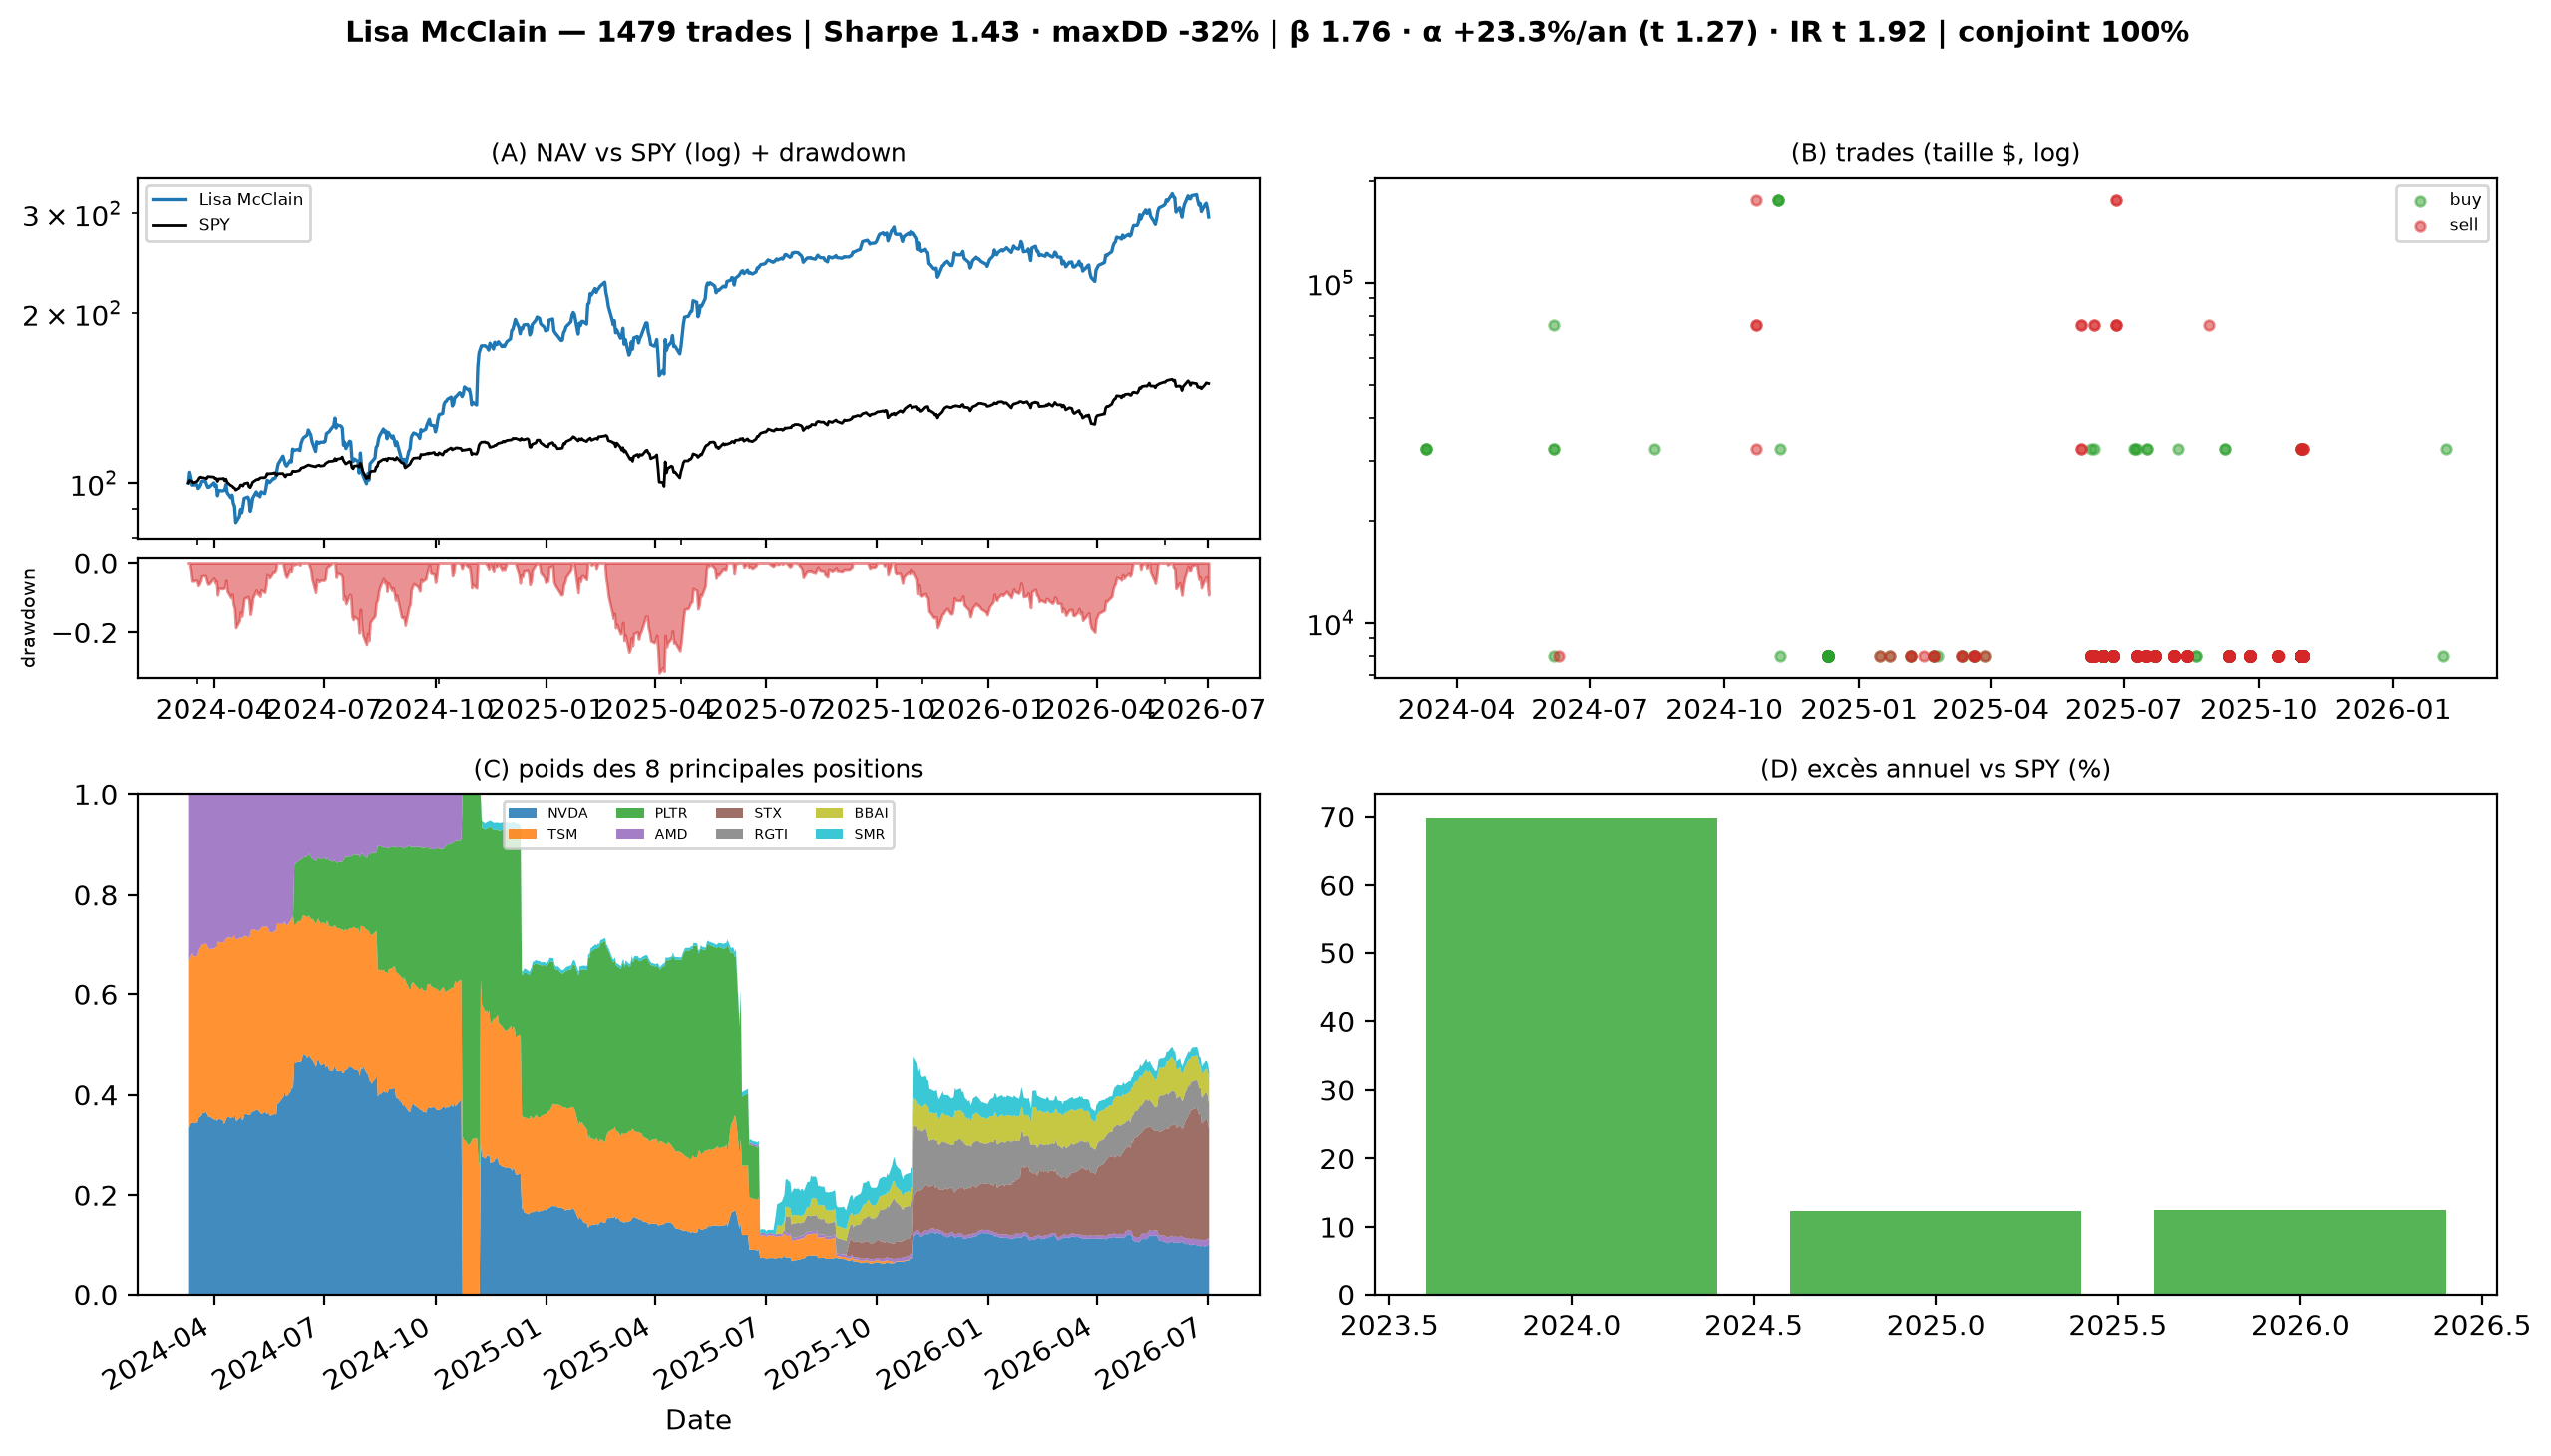
\includegraphics[width=0.98\textwidth,height=0.74\textheight,keepaspectratio]{png/figs_pop/G_M001136_portrait.png}\\[1mm]
  \kpi{helec}{1\,479 trades · IR t 1,92}{$+41\,\%$/an d'excès}\hspace{8mm}%
  \kpi{alertred}{$\beta$ 1,76 → $t_{\text{appr}}$ 1,27}{l'excès, c'est du levier, pas du talent}
\end{frame}

\begin{frame}{Raul Ruiz — « significatif » à l'appraisal sur 10 trades : un faux positif}
  \centering
  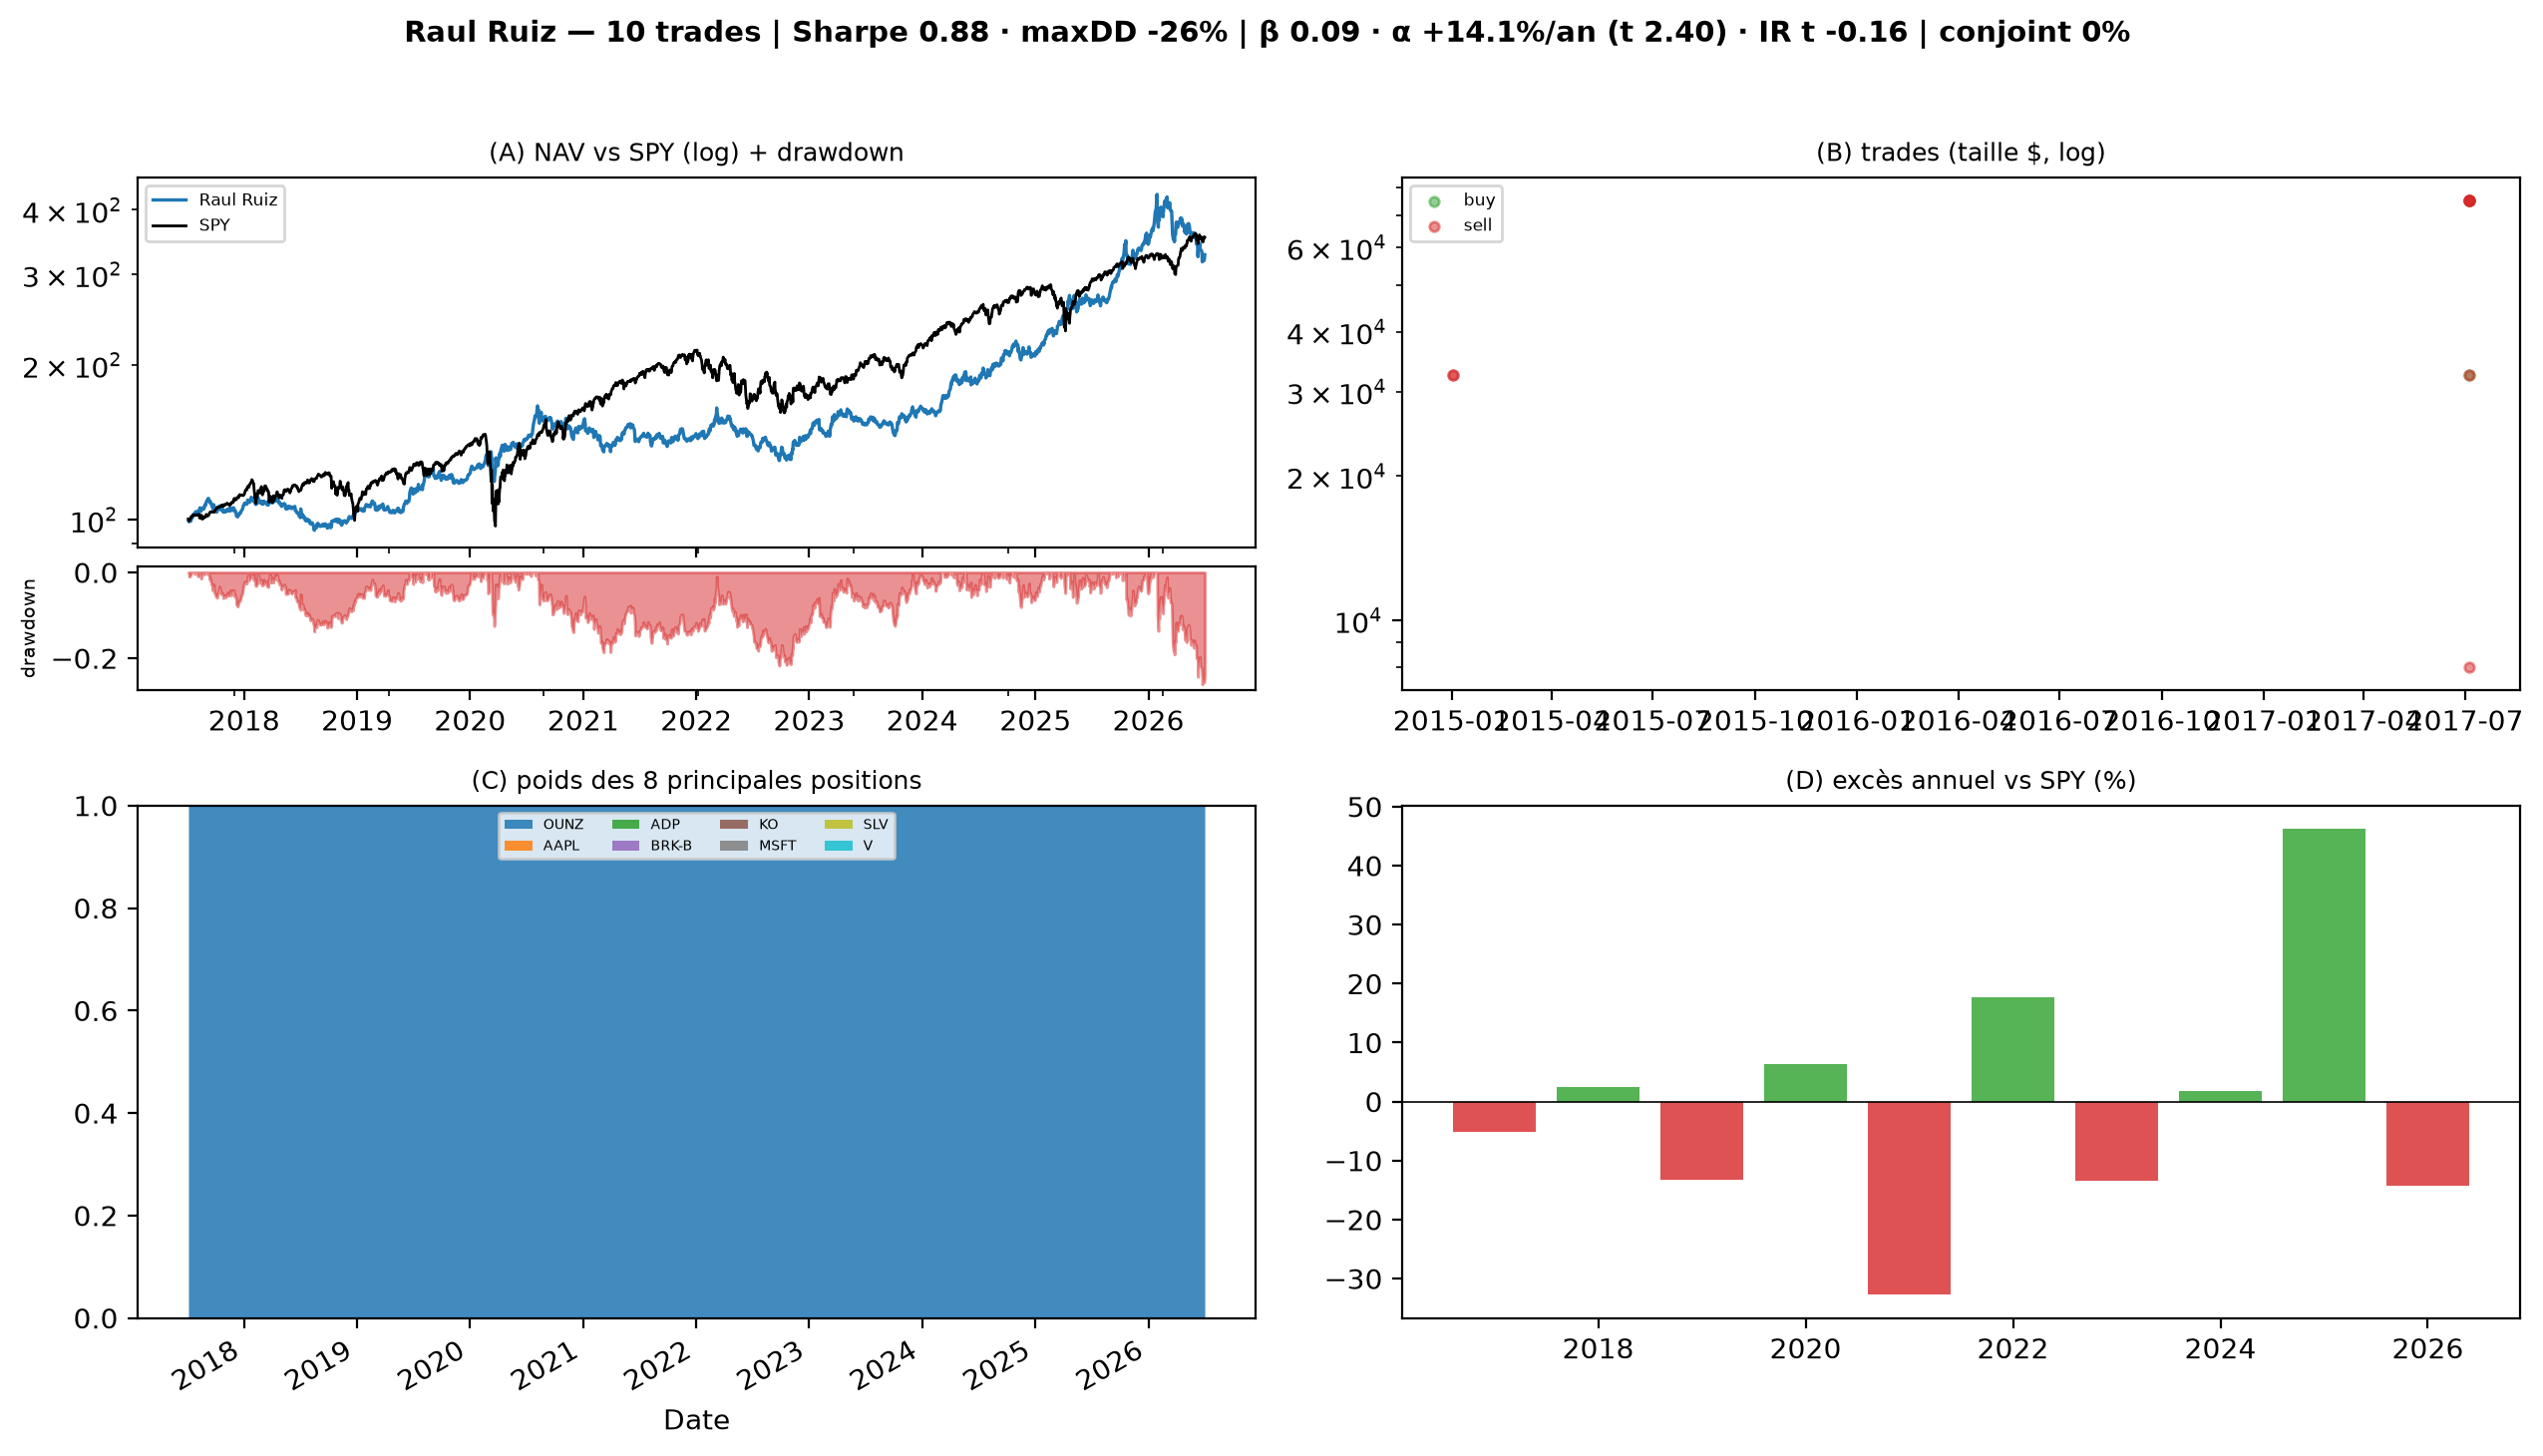
\includegraphics[width=0.98\textwidth,height=0.74\textheight,keepaspectratio]{png/figs_pop/G_R000599_portrait.png}\\[1mm]
  \kpi{warnorange}{appraisal t 2,40}{« significatif »\ldots}\hspace{8mm}%
  \kpi{alertred}{10 trades · $\beta$ 0,09}{0\,\% de trades gagnants : un faux positif}
\end{frame}

\begin{frame}{David Trott — 8\,\% de trades gagnants, $-9\,\%$/an}
  \centering
  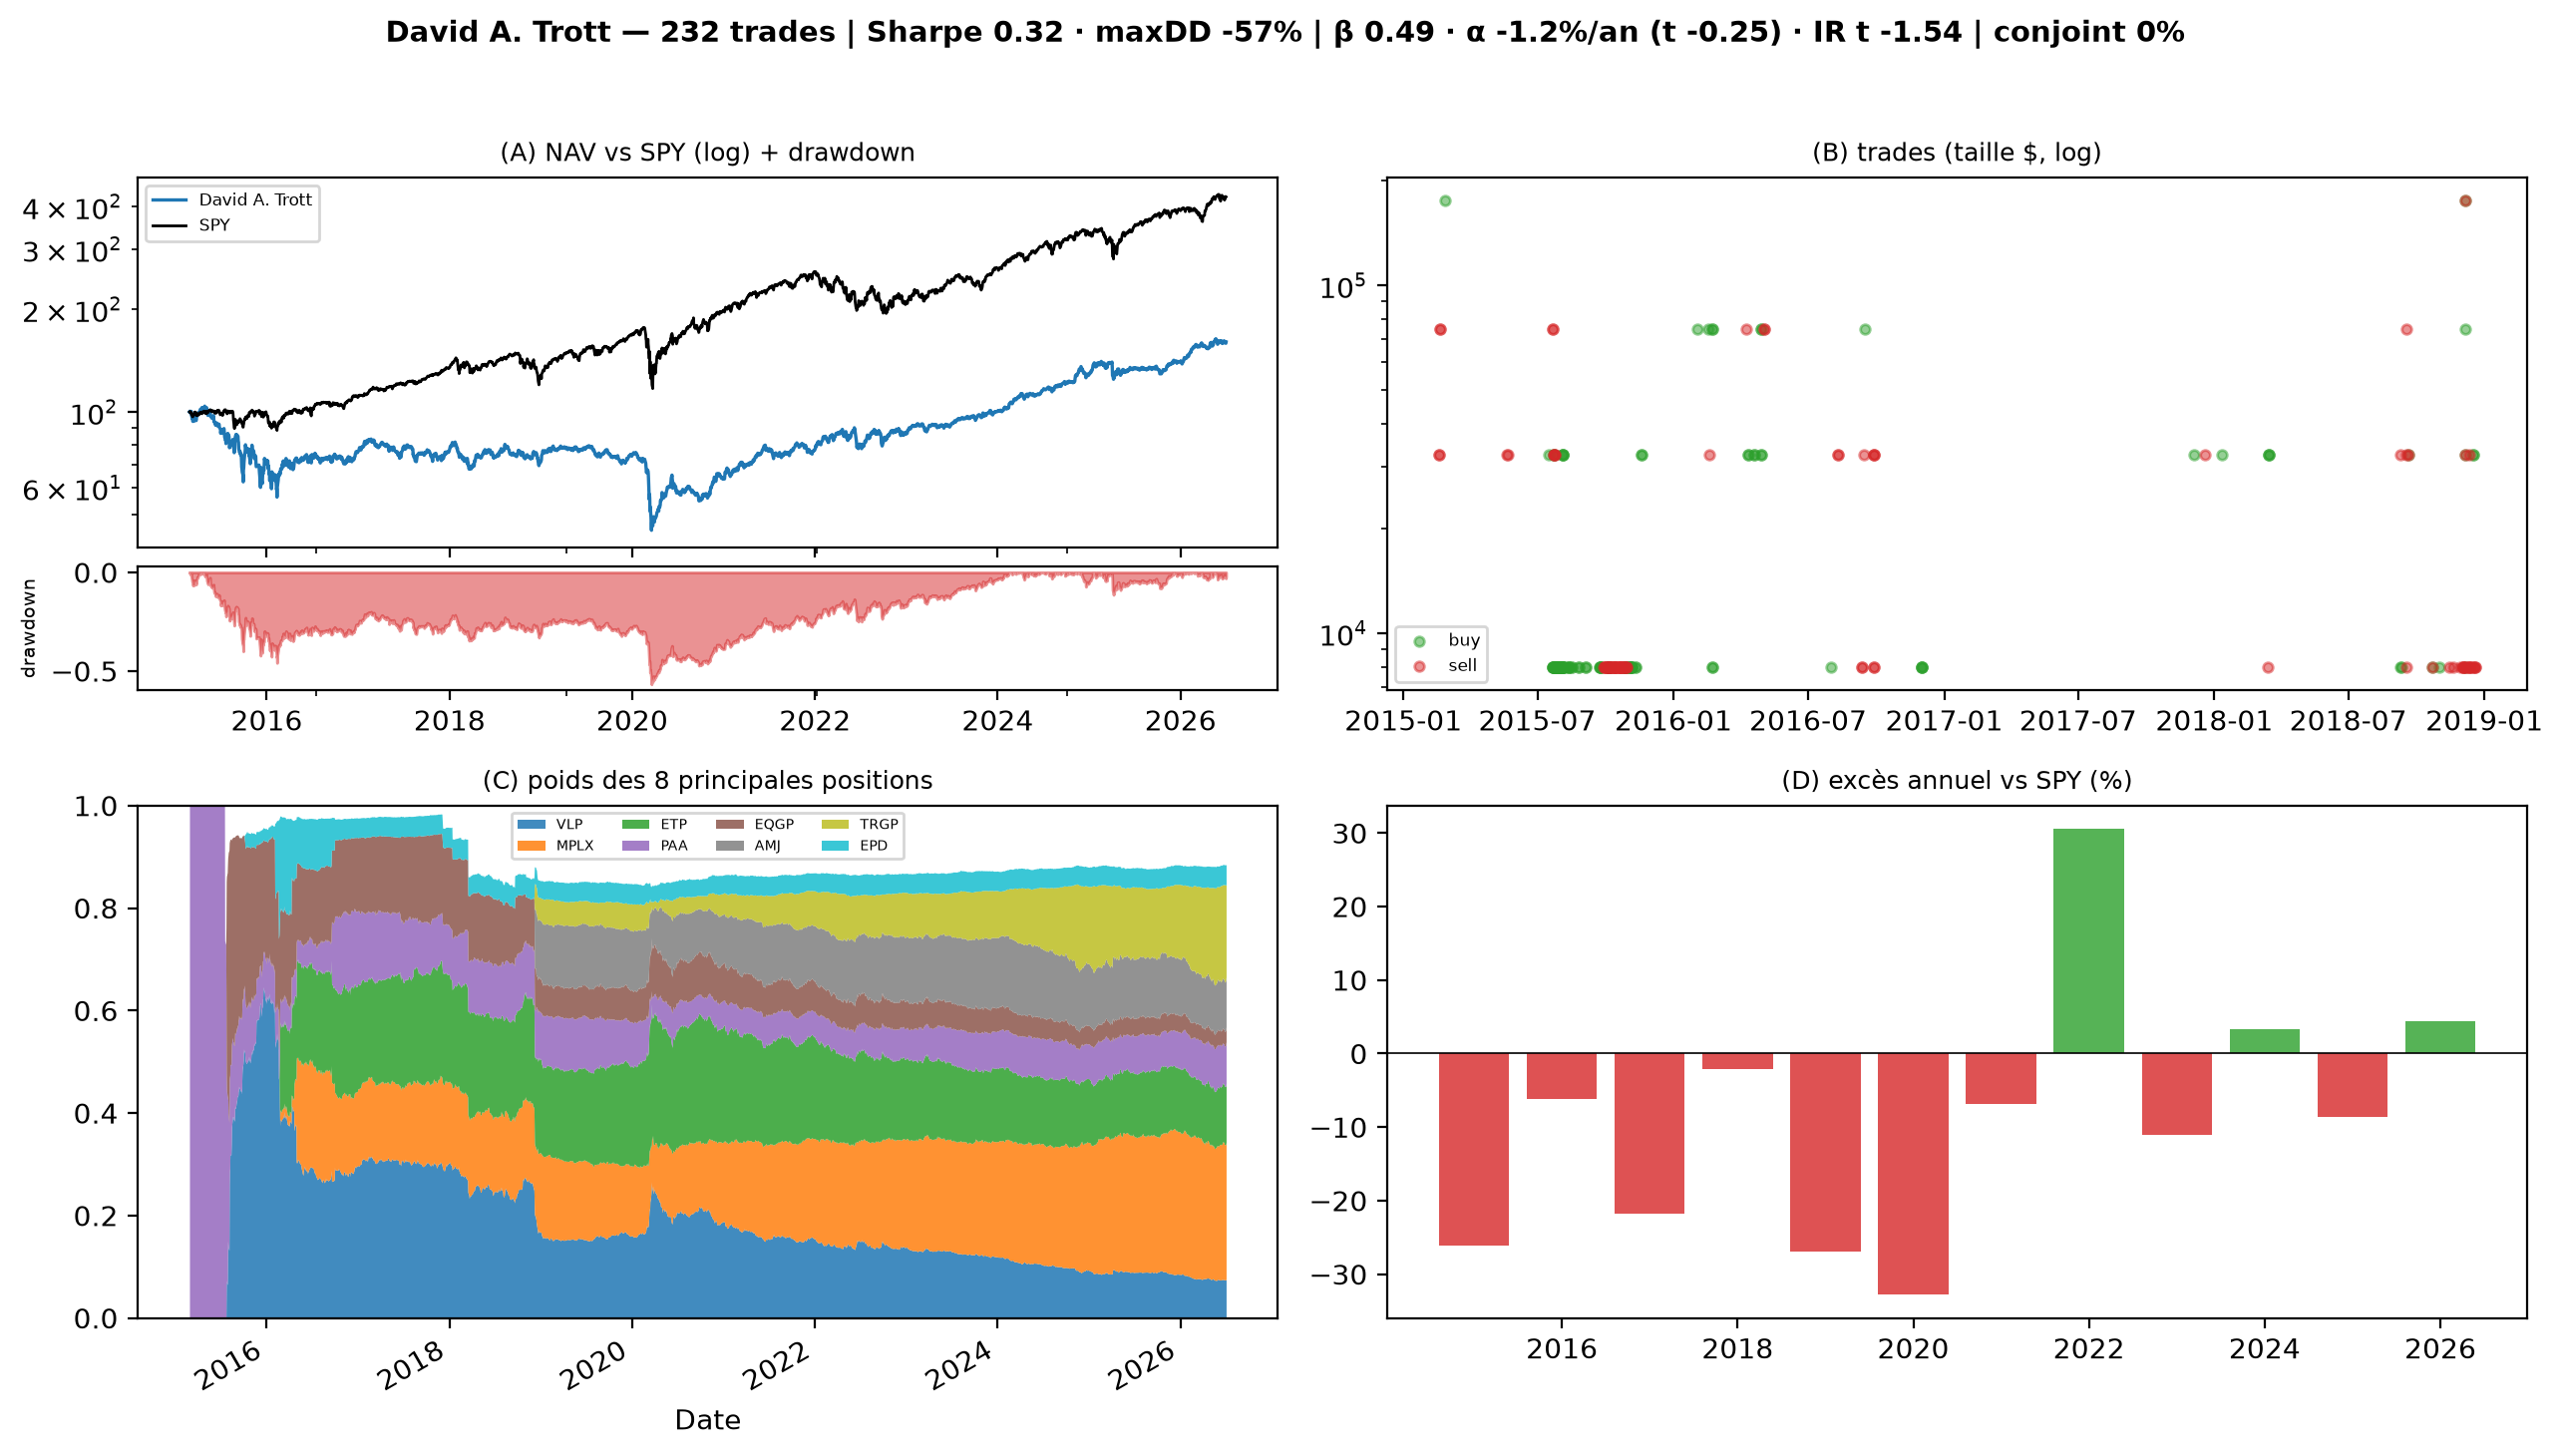
\includegraphics[width=0.98\textwidth,height=0.74\textheight,keepaspectratio]{png/figs_pop/G_T000475_portrait.png}\\[1mm]
  \kpi{alertred}{8\,\%}{de ses achats battent le marché}\hspace{8mm}%
  \kpi{alertred}{$-9{,}4\,\%$/an · PF 0,08}{l'autre extrême du classement}
\end{frame}

\begin{frame}{Richard Burr — les ventes de février 2020 (enquête COVID)}
  \centering
  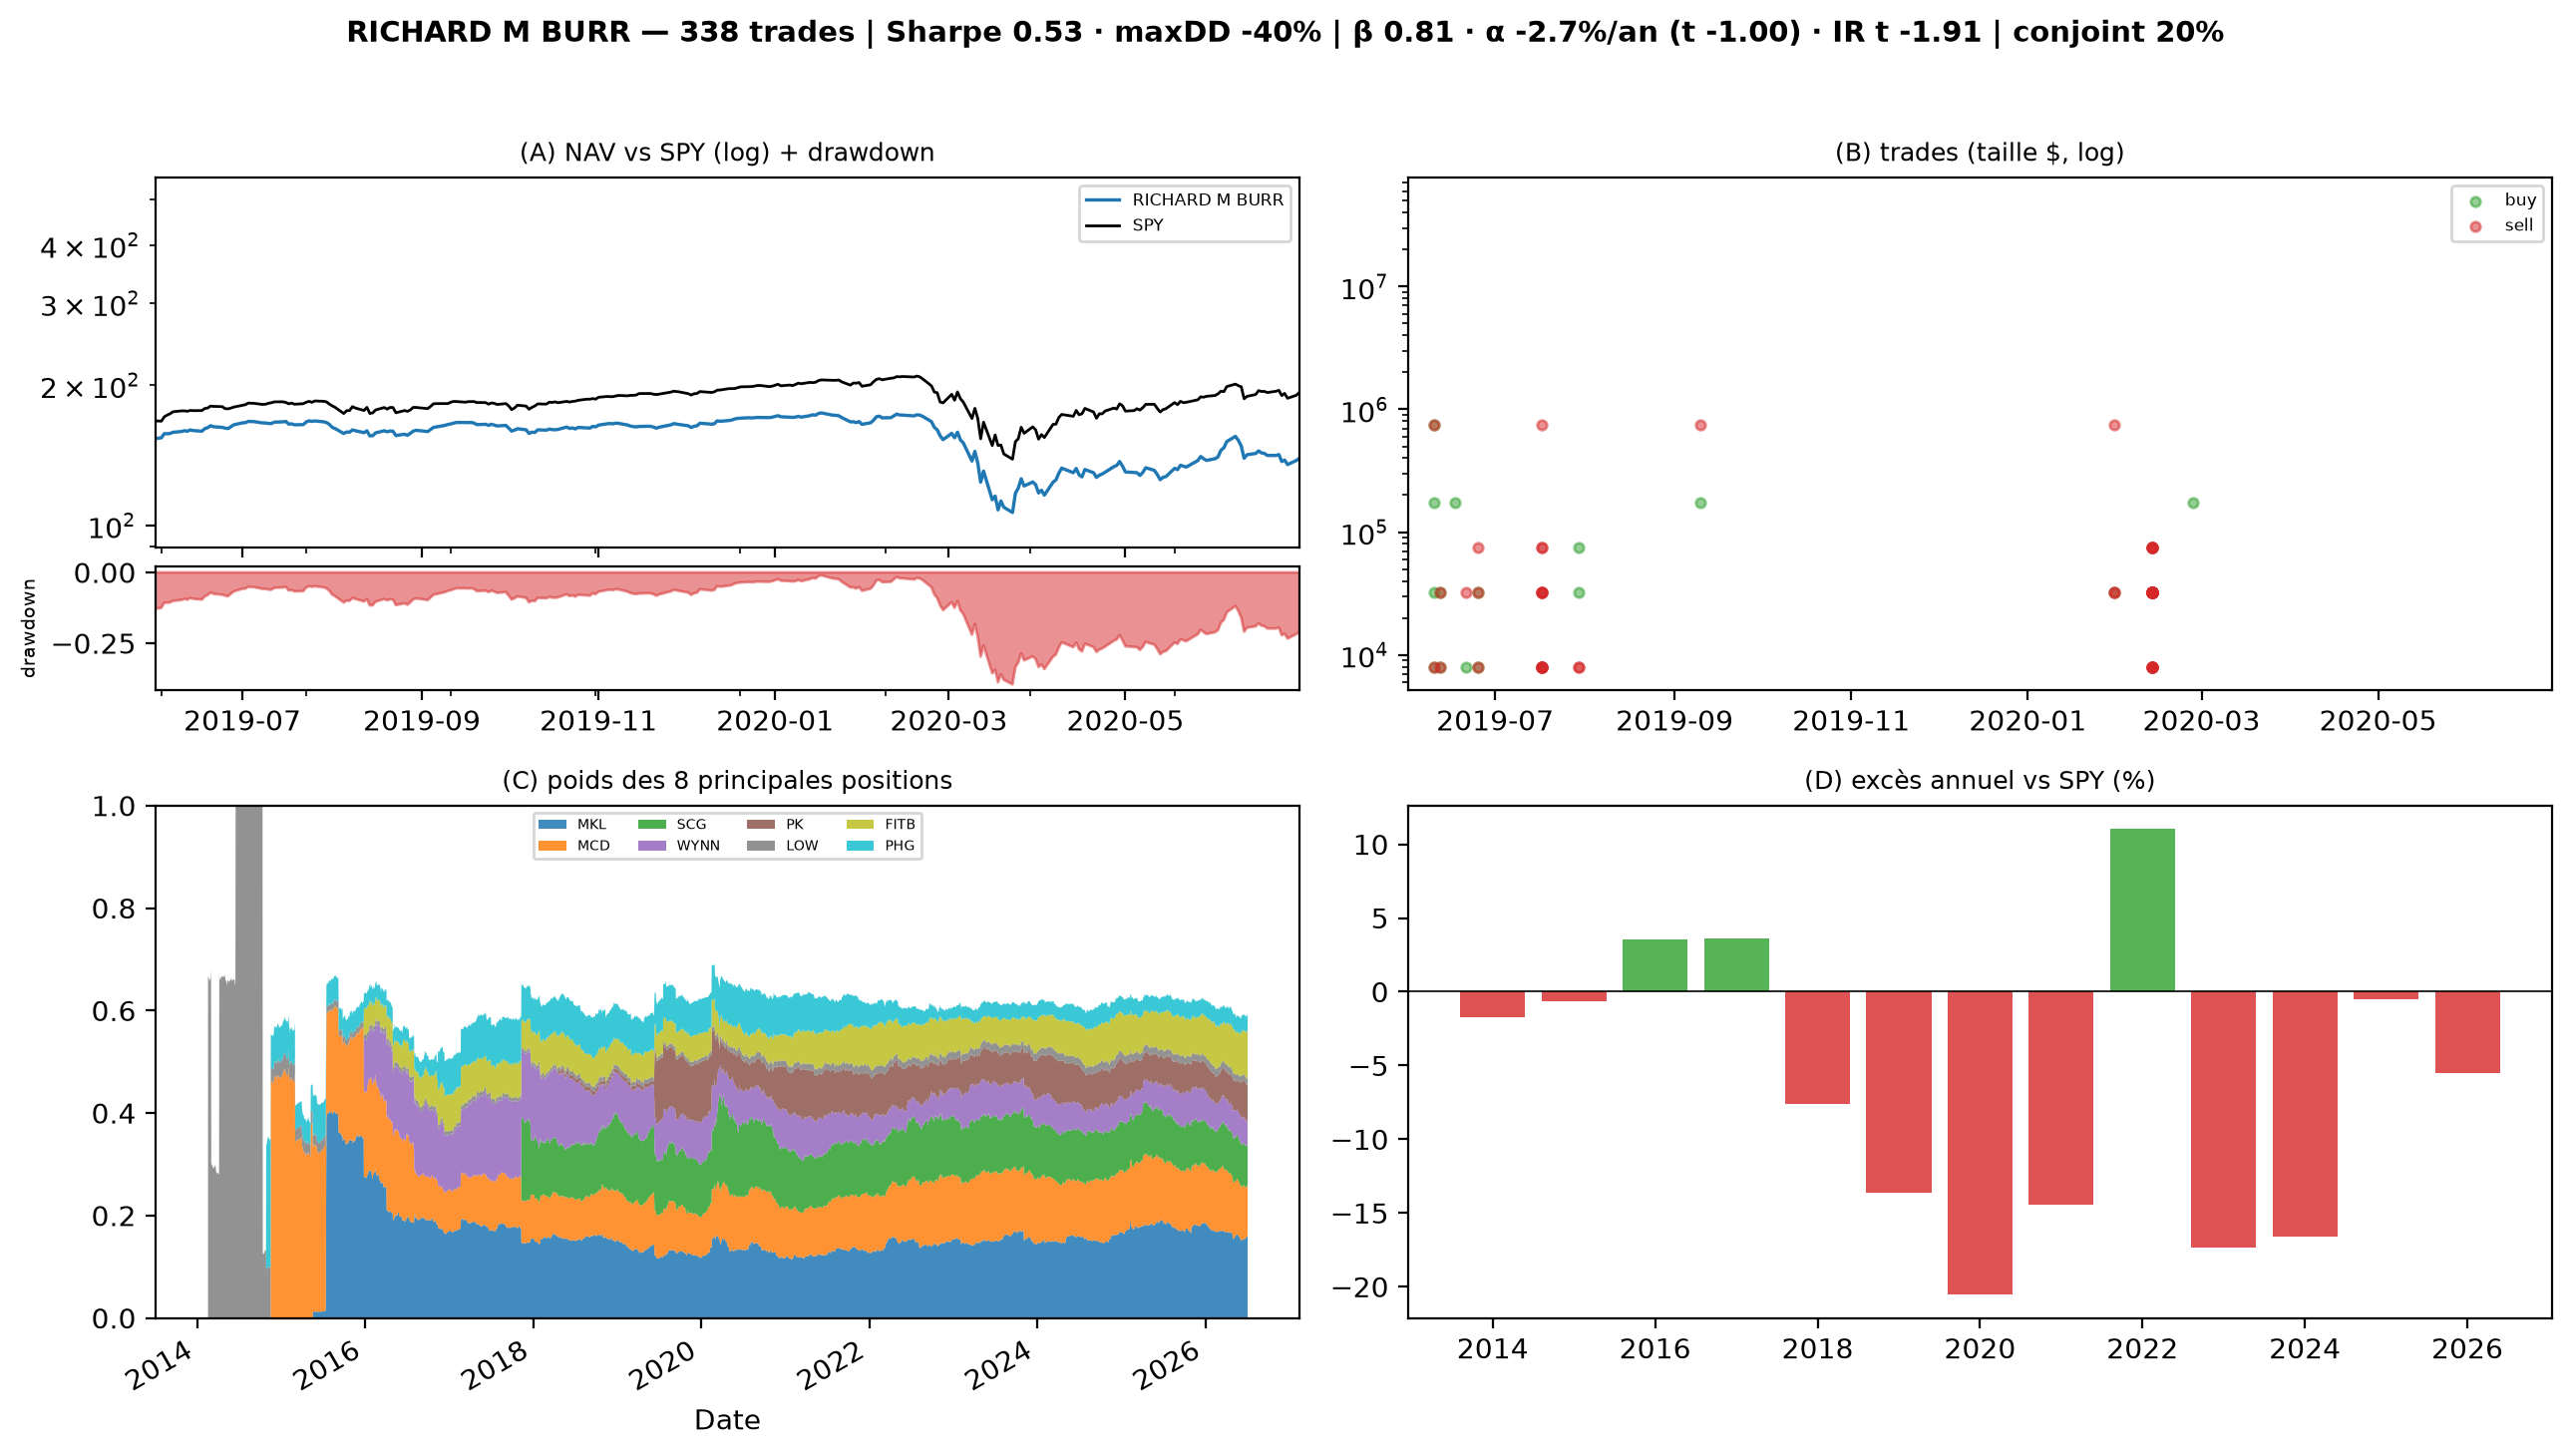
\includegraphics[width=0.98\textwidth,height=0.74\textheight,keepaspectratio]{png/figs_pop/G_B001135_portrait.png}\\[1mm]
  \defl{ventes juste avant le krach (zoom juin 2019 – juin 2020) ; enquêtes DOJ/SEC classées sans charge — le cas éthique, hors performance.}
\end{frame}

\begin{frame}{La galerie en chiffres — les 8 portraits}
  \centering
  {\footnotesize
  \begin{tabular}{@{}l l r r r r r r@{}}
    \toprule
    Membre & profil & Sharpe & $\beta$ & $\alpha$\,\%/an (t) & hit & PF & excès/an\\\midrule
    Pelosi     & médiatisée       & 0,77 & 1,12 & $+2{,}6$ (0,64)    & 63\,\% & 2,39 & $+3{,}4\,\%$\\
    Khanna     & médiatisé        & 0,87 & 0,98 & $+0{,}6$ (0,36)    & 40\,\% & 0,88 & $+0{,}2\,\%$\\
    Fetterman  & 1\up{er} IR/appr & 2,90 & 1,17 & $+40{,}2$ (\textbf{2,38}) & 44\,\% & 6,42 & $+54{,}7\,\%$\\
    Whitehouse & signif. robuste  & 1,02 & 1,04 & $+5{,}0$ (1,85)    & 45\,\% & 1,42 & $+5{,}7\,\%$\\
    McClain    & IR gonflé $\beta$ & 1,43 & 1,76 & $+23{,}3$ (1,27)  & 30\,\% & 0,80 & $+40{,}9\,\%$\\
    Ruiz       & faux positif     & 0,88 & 0,09 & $+14{,}1$ (\textbf{2,40}) & \phantom{0}0\,\% & 0,00 & $-1{,}0\,\%$\\
    Trott      & extrême bas      & 0,32 & 0,49 & $-1{,}2$ ($-$0,25) & \phantom{0}8\,\% & 0,08 & $-9{,}4\,\%$\\
    Burr       & médiatisé        & 0,53 & 0,81 & $-2{,}7$ ($-$1,00) & 46\,\% & 0,70 & $-6{,}1\,\%$\\
    \bottomrule
  \end{tabular}}\\[2mm]
  \kpi{helec}{deux}{$|t|>2$ (Fetterman \& Ruiz) — tous deux sur 10 trades}\hspace{6mm}%
  \kpi{grisC}{aucun}{signal copiable qui ressort}\\[1.5mm]
  \defl{$x_j$ = excès d'un achat vs SPY sur sa fenêtre de détention · \textbf{hit} $=$ part des achats où $x_j>0$ · \textbf{PF} $=\bigl(\textstyle\sum x_j^{+}\bigr)\big/\bigl|\textstyle\sum x_j^{-}\bigr|$, plafonné à 10.}\\[1mm]
  \repband{des styles radicalement différents, des chiffres parfois spectaculaires — mais aucun ne passe le seuil de façon crédible : on mesure des personnes, pas « le Congrès ».}
\end{frame}

\section{Partie III · Les autres dépôts}
\partdivider{dataC}{PARTIE III}{Les autres dépôts}{au-delà des PTR : le patrimoine, sa reconstruction, sa vérification --- Chambre}

% ══════════════════════════════════════════════════════════════════════════
%  Arc : le problème → le catalogue (2) → ce qu'ils apportent (2) →
%        reconstruire (3) → vérifier (2) → les cas → le bilan → teaser
%  Chiffres re-sourcés sur 01_autres_filing_types/cache/tables/*.csv + ANALYSE_FILING_TYPES_HOUSE.md
% ══════════════════════════════════════════════════════════════════════════

% ── III.1 · Le problème ──────────────────────────────────────────────────
\begin{frame}{Le problème --- un type de dépôt lu sur douze}
  \begin{columns}[c]
    \begin{column}{0.40\textwidth}\centering
      \colorbox{okgreen!18}{\parbox{0.92\linewidth}{\centering\footnotesize\vspace{0.4mm}
        \textbf{\large 8\,267} PTR (\co{P})\\{\scriptsize le seul type lu jusqu'ici}\vspace{0.4mm}}}\\[2mm]
      \colorbox{grisC!12}{\parbox{0.92\linewidth}{\centering\footnotesize\vspace{0.4mm}
        \textbf{\large 27\,110} autres dépôts\\{\scriptsize \textbf{11 types}, jamais lus\\(sur 35\,377 recensés)}\vspace{0.4mm}}}
    \end{column}
    \begin{column}{0.58\textwidth}
      {\footnotesize\textbf{L'angle mort} --- d'où viennent les titres détenus à la
       \emph{sortie} d'un mandat ?}\\[1.5mm]
      \begin{tikzpicture}[node distance=1.6mm]
        \node[rectangle, rounded corners=2pt, draw=alertred, fill=alertred, line width=0.8pt,
              align=left, font=\scriptsize, text width=6.4cm, minimum height=0.68cm] (a)
          {\color{white}\textbf{33,2\,\%} déjà détenus \textbf{à l'entrée} --- \textbf{invisibles} d'un backtest qui part de zéro};
        \node[bande=helec, text width=6.4cm, below=of a] (b)
          {\textbf{45,5\,\%} achetés en cours de mandat --- vus par les PTR};
        \node[bande=grisC, text width=6.4cm, below=of b] (c)
          {\textbf{21,3\,\%} restaient à expliquer};
      \end{tikzpicture}\\[1.5mm]
      \choixbox{un tiers du patrimoine de sortie n'a \textbf{jamais} été tradé pendant
       le mandat : sans le patrimoine d'\textbf{entrée}, il est perdu. C'est ce que les
       \textbf{autres dépôts} vont nous rendre.}
    \end{column}
  \end{columns}
\end{frame}

% ── III.2 · Le catalogue : la famille patrimoine (O/C/H/T/A) ─────────────
\begin{frame}{1 · Le catalogue --- à quoi correspond chaque type}
  \centering
  {\footnotesize cinq types, un socle commun (le \emph{Financial Disclosure Report}) --- les
   \textbf{transactions (Schedule B) n'existent que dans \co{O}, \co{T} et leurs amendements \co{A}} :}\\[2mm]
  \begin{columns}[T]
    \begin{column}{0.19\textwidth}\centering
      \href{https://disclosures-clerk.house.gov/public_disc/financial-pdfs/2023/10059952.pdf}{\fcolorbox{black!30}{white}{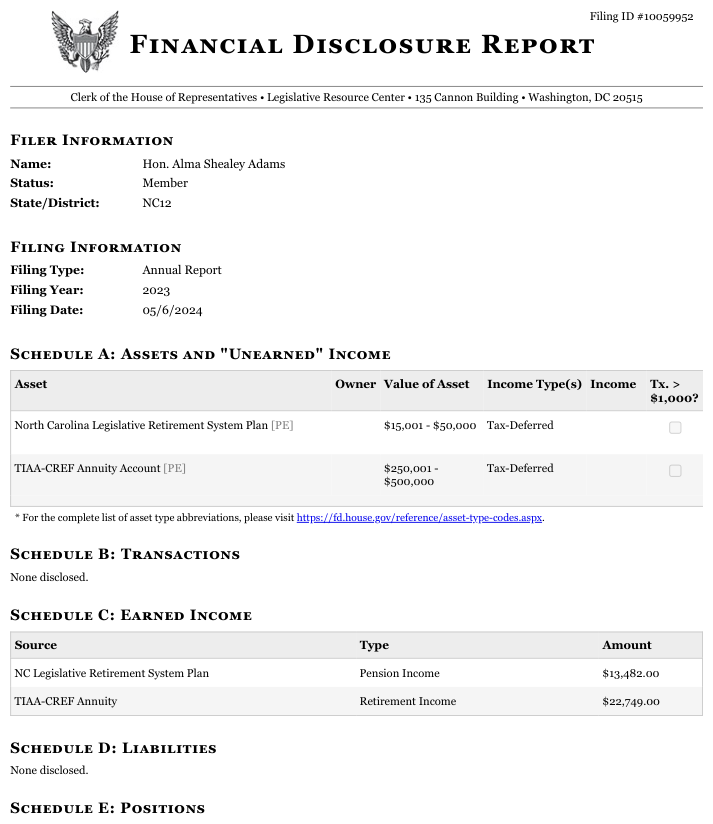
\includegraphics[height=29mm]{png/figs_deck/ftype_o.png}}}\\[0.8mm]
      {\footnotesize\textbf{O — Annual}}\\{\scriptsize bilan annuel · \textbf{4\,626}}
    \end{column}
    \begin{column}{0.19\textwidth}\centering
      \href{https://disclosures-clerk.house.gov/public_disc/financial-pdfs/2023/10056211.pdf}{\fcolorbox{black!30}{white}{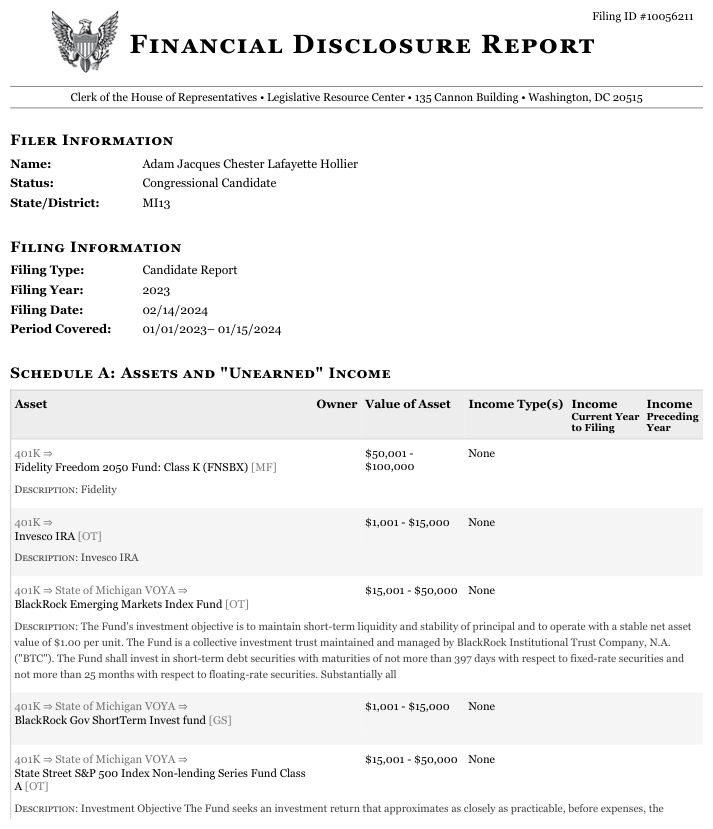
\includegraphics[height=29mm]{png/figs_deck/ftype_c.png}}}\\[0.8mm]
      {\footnotesize\textbf{C — Candidate}}\\{\scriptsize candidat · \textbf{10\,129}}
    \end{column}
    \begin{column}{0.19\textwidth}\centering
      \href{https://disclosures-clerk.house.gov/public_disc/financial-pdfs/2023/10062638.pdf}{\fcolorbox{black!30}{white}{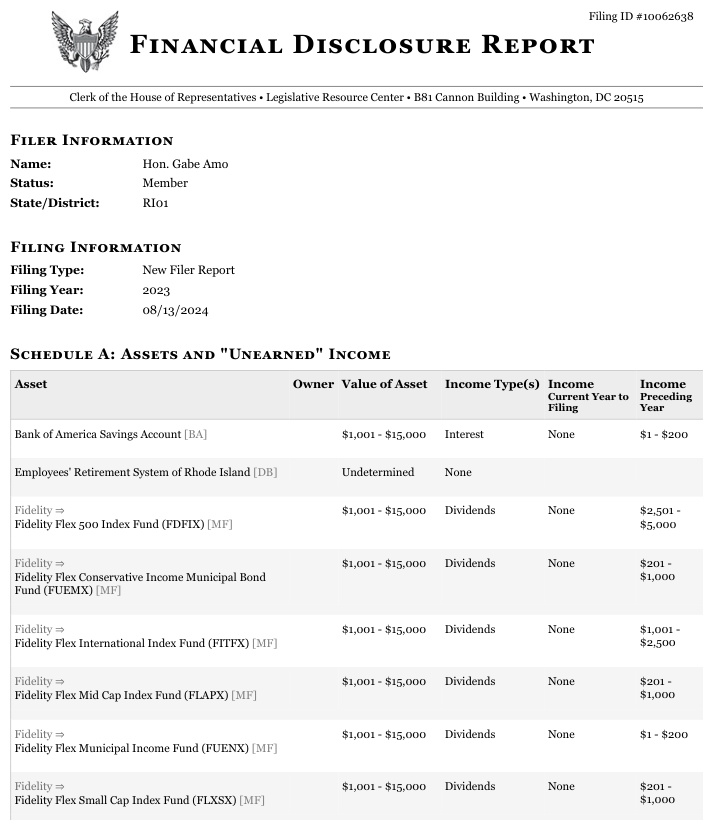
\includegraphics[height=29mm]{png/figs_deck/ftype_h.png}}}\\[0.8mm]
      {\footnotesize\textbf{H — New Filer}}\\{\scriptsize 1\iere{} déclaration · \textbf{395}}
    \end{column}
    \begin{column}{0.19\textwidth}\centering
      \href{https://disclosures-clerk.house.gov/public_disc/financial-pdfs/2023/10050798.pdf}{\fcolorbox{black!30}{white}{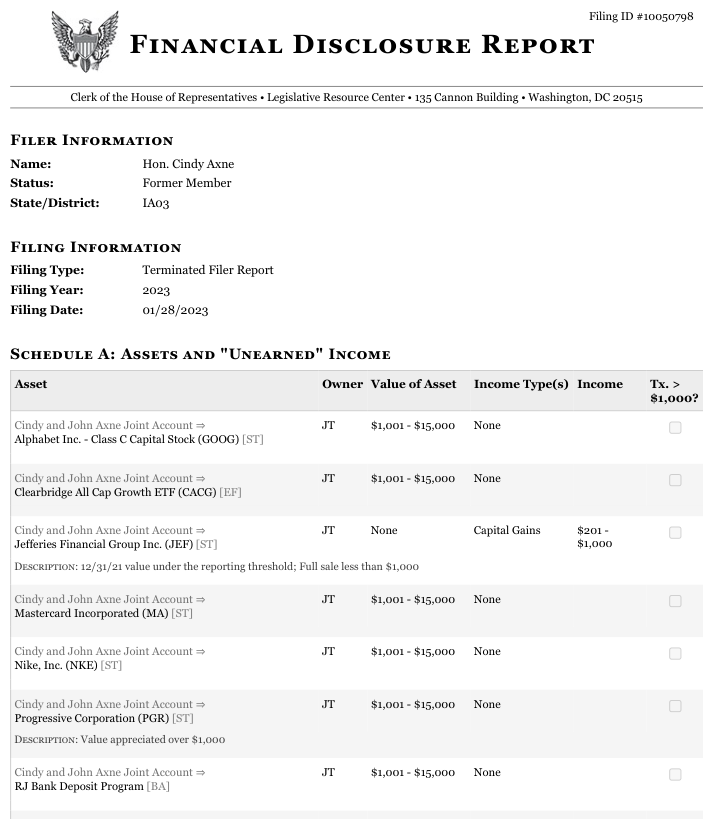
\includegraphics[height=29mm]{png/figs_deck/ftype_t.png}}}\\[0.8mm]
      {\footnotesize\textbf{T — Termination}}\\{\scriptsize départ · \textbf{394}}
    \end{column}
    \begin{column}{0.19\textwidth}\centering
      \href{https://disclosures-clerk.house.gov/public_disc/financial-pdfs/2023/10062190.pdf}{\fcolorbox{black!30}{white}{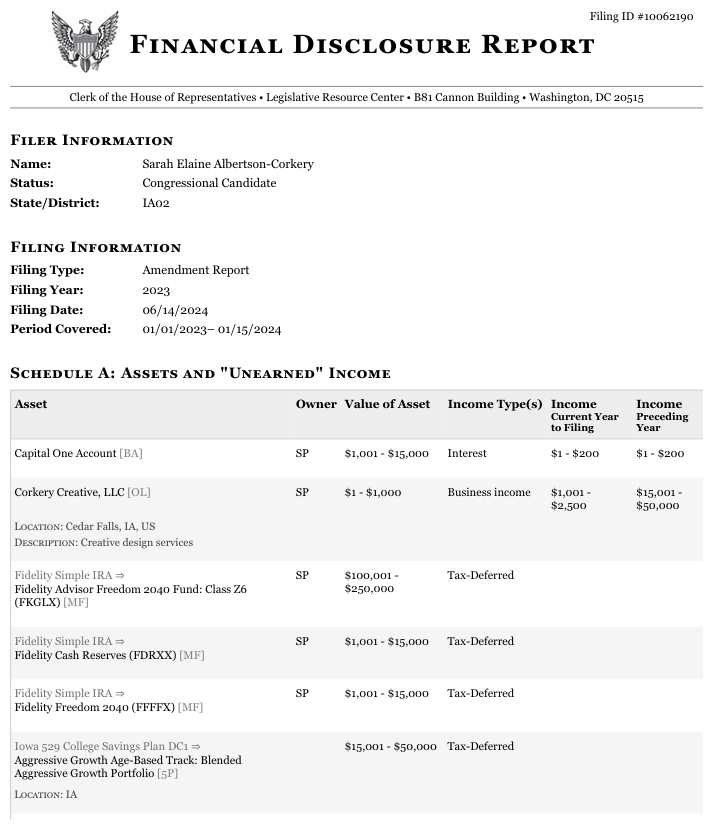
\includegraphics[height=29mm]{png/figs_deck/ftype_a.png}}}\\[0.8mm]
      {\footnotesize\textbf{A — Amendment}}\\{\scriptsize correction · \textbf{2\,305}}
    \end{column}
  \end{columns}
  \vspace{2.5mm}
  \badge{dataC}{chaque vignette est cliquable → ouvre le vrai document}\quad
  {\scriptsize\color{black!60} le chiffre sous chaque type = \textbf{nombre de dépôts} recensés · significations vérifiées en ouvrant les documents}
\end{frame}

% ── III.3 · Le catalogue : les types sans transaction (X/D/W/E/G + B) ────
\begin{frame}{1 · Le catalogue --- les types sans transaction}
  \centering
  {\footnotesize cinq types \textbf{sans aucune transaction} :}\quad{\scriptsize\color{black!55} chaque vignette ouvre le vrai PDF}\\[1.5mm]
  \begin{columns}[T]
    \begin{column}{0.19\textwidth}\centering
      \href{https://disclosures-clerk.house.gov/public_disc/financial-pdfs/2023/30019473.pdf}{\fcolorbox{black!30}{white}{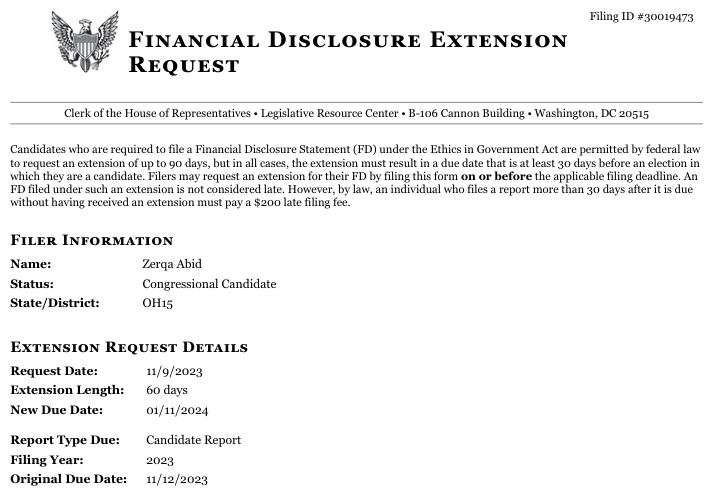
\includegraphics[height=21mm]{png/figs_deck/ftype_x.png}}}\\[0.6mm]
      {\scriptsize\textbf{X — Extension}\\demande de délai}
    \end{column}
    \begin{column}{0.19\textwidth}\centering
      \href{https://disclosures-clerk.house.gov/public_disc/financial-pdfs/2023/40003491.pdf}{\fcolorbox{black!30}{white}{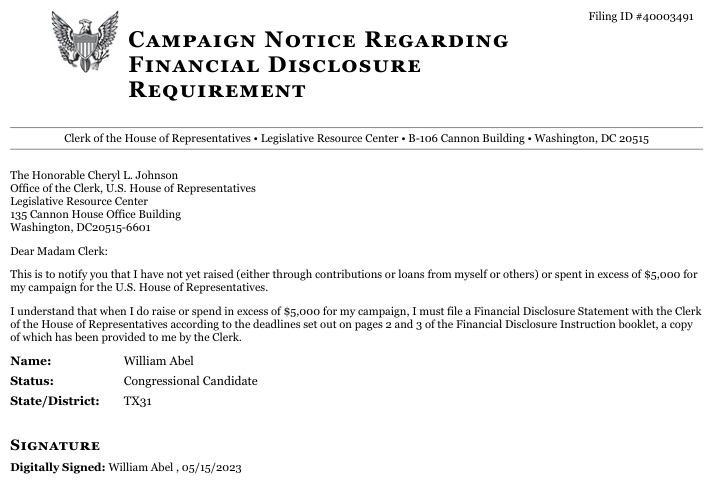
\includegraphics[height=21mm]{png/figs_deck/ftype_d.png}}}\\[0.6mm]
      {\scriptsize\textbf{D — Campaign Notice}\\« < 5\,000 \$ »}
    \end{column}
    \begin{column}{0.19\textwidth}\centering
      \href{https://disclosures-clerk.house.gov/public_disc/financial-pdfs/2023/8219940.pdf}{\fcolorbox{black!30}{white}{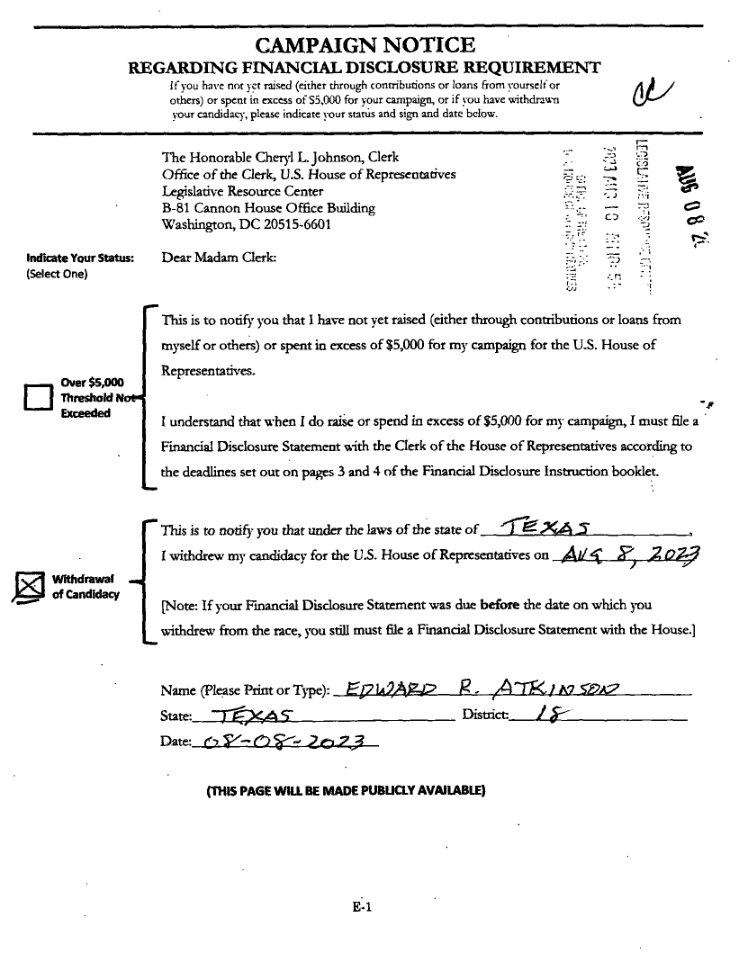
\includegraphics[height=21mm]{png/figs_deck/ftype_w.png}}}\\[0.6mm]
      {\scriptsize\textbf{W — idem, papier}\\(ou retrait)}
    \end{column}
    \begin{column}{0.19\textwidth}\centering
      \href{https://disclosures-clerk.house.gov/public_disc/financial-pdfs/2023/8219324.pdf}{\fcolorbox{black!30}{white}{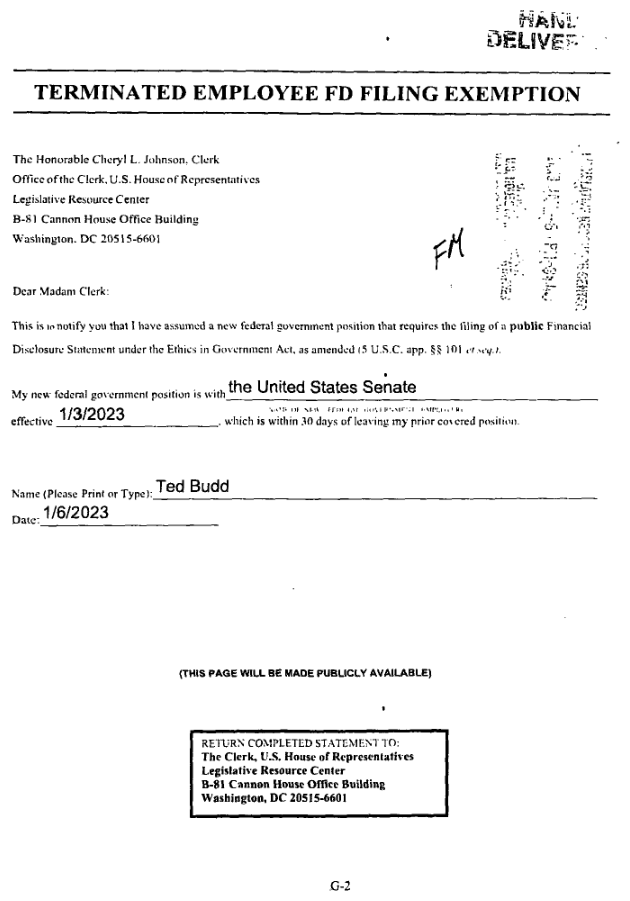
\includegraphics[height=21mm]{png/figs_deck/ftype_e.png}}}\\[0.6mm]
      {\scriptsize\textbf{E — Exemption}\\départ, poste fédéral}
    \end{column}
    \begin{column}{0.19\textwidth}\centering
      \href{https://disclosures-clerk.house.gov/public_disc/financial-pdfs/2023/8219737.pdf}{\fcolorbox{black!30}{white}{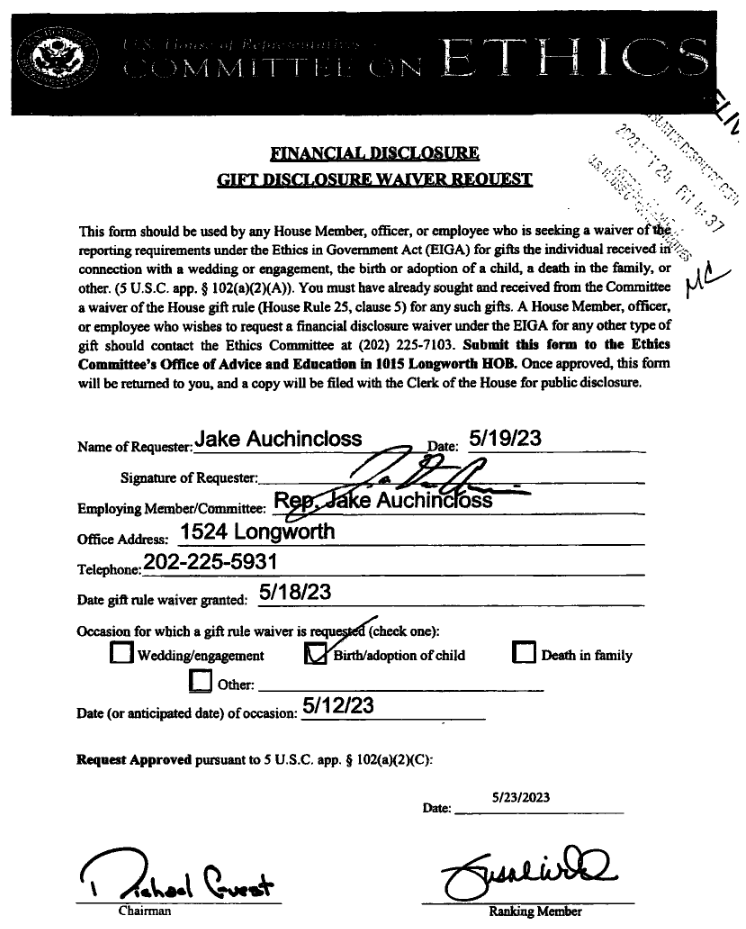
\includegraphics[height=21mm]{png/figs_deck/ftype_g.png}}}\\[0.6mm]
      {\scriptsize\textbf{G — Gift Waiver}\\dérogation cadeau}
    \end{column}
  \end{columns}
  \vspace{2.5mm}
  \begin{columns}[c]
    \begin{column}{0.14\textwidth}\centering
      \href{https://disclosures-clerk.house.gov/public_disc/financial-pdfs/2023/8219364.pdf}{\fcolorbox{alertred}{white}{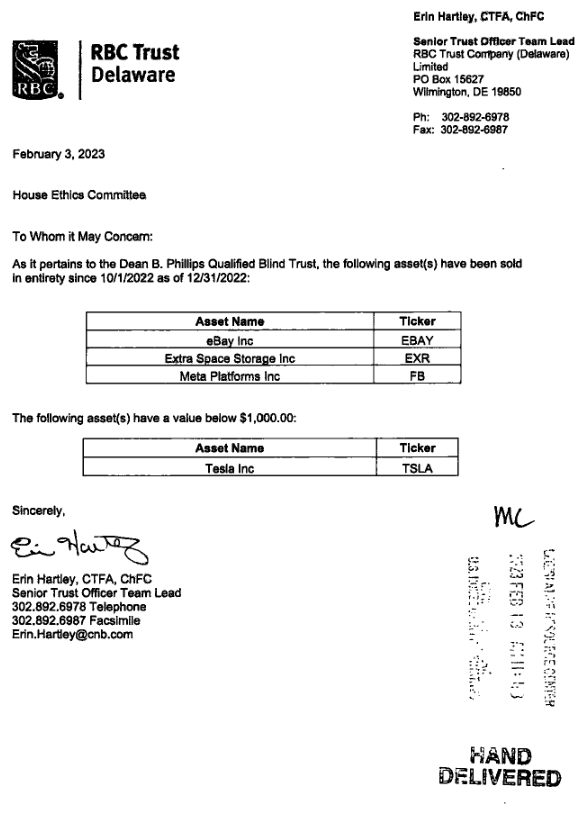
\includegraphics[height=20mm]{png/figs_deck/ftype_b.png}}}
    \end{column}
    \begin{column}{0.82\textwidth}
      \colorbox{alertred!10}{\parbox{0.97\linewidth}{\footnotesize\raggedright\vspace{0.5mm}
        \textbf{\textcolor{alertred}{B — Blind Trust}} (23 dépôts) : la banque du \emph{trust}
        liste de vraies ventes (eBay, Meta, Tesla…), mais \textbf{pas décidées par l'élu} :
        la fiducie aveugle (cf.\ le cas Phillips, plus loin).\vspace{0.5mm}}}
    \end{column}
  \end{columns}
\end{frame}

% ── III.2 · Le catalogue : la vie déclarative (frise cycle de vie) ───────
\begin{frame}{1 · Le catalogue --- la vie déclarative d'un élu}
  \centering
  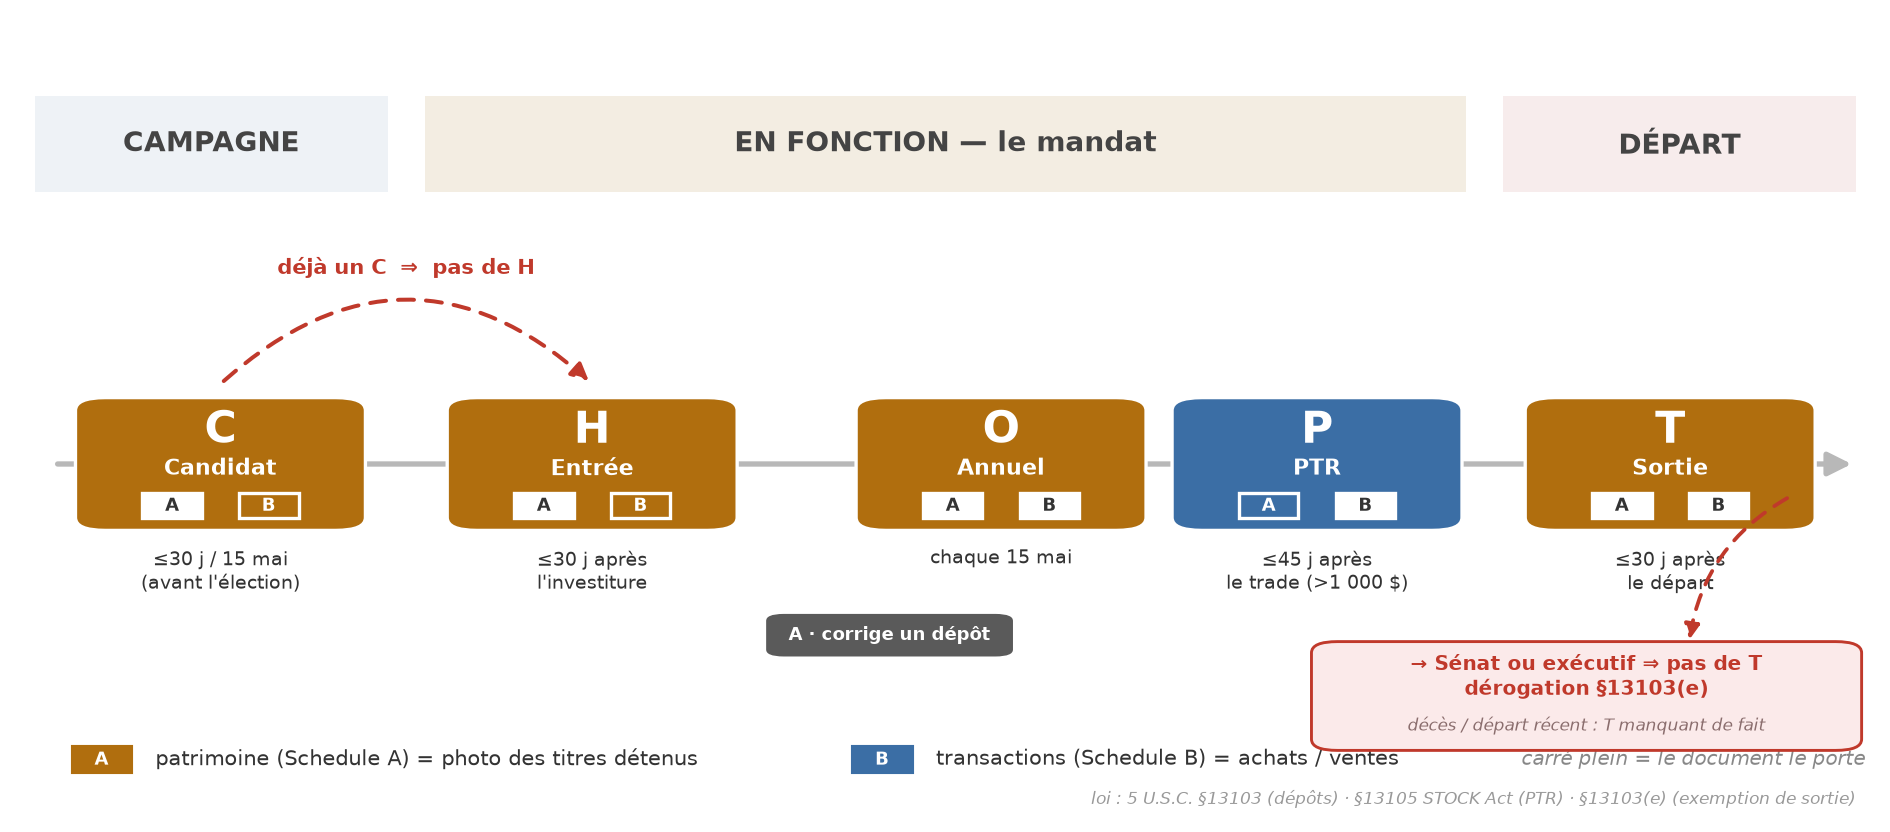
\includegraphics[width=0.84\textwidth]{png/figs_deck/fig_house_loi_cycle.png}\\[1mm]
  {\footnotesize les \textbf{photos} (\co{C}\,·\,\co{H}\,·\,\co{O}\,·\,\co{T}) disent ce qu'il
   \textbf{possède}, le \co{P} ce qu'il \textbf{fait} --- chaque étape a son dépôt \textbf{et son
   délai légal}}
\end{frame}

% ── III.3a-bis · couverture des entrées/sorties (remontée de l'annexe A7) ────
\begin{frame}{La couverture des entrées et des sorties (Chambre)}
  \centering\vspace{2mm}
  {\footnotesize
  \begin{tabular}{@{}p{0.22\linewidth} p{0.62\linewidth}@{}}
    \toprule
    \textbf{470 entrées} depuis 2014 & 82\,\% ont déposé un \textbf{H} (photo d'entrée) ·
      16\,\% un \textbf{C} à la place → \textbf{98\,\% couverts} \\
    \midrule
    \textbf{463 sorties} définitives & 81\,\% ont déposé un \textbf{T} (photo de sortie) ;
      les 86 sans T : partis au Sénat/exécutif (dispensés), décès \\
    \bottomrule
  \end{tabular}}\\[3mm]
  {\footnotesize la photo d'entrée : \textbf{252} ancrés par un H · \textbf{32} par un C
   = \textbf{284} portefeuilles d'entrée datés}
\end{frame}

% ── III.3b · Le catalogue : les sections du formulaire (Schedule A/B) ────
\begin{frame}{1 · Le catalogue --- le même formulaire, des sections en commun}
  \centering
  {\footnotesize un dépôt est découpé en \textbf{Schedules} --- des sections, de \co{A} à \co{J} ---
   chacune sa catégorie : \co{A} patrimoine · \co{B} transactions · \co{C} revenus · \co{D} dettes
   · \co{E} postes… ; la matrice montre \textbf{lesquelles apparaissent selon le type} :}\\[1mm]
  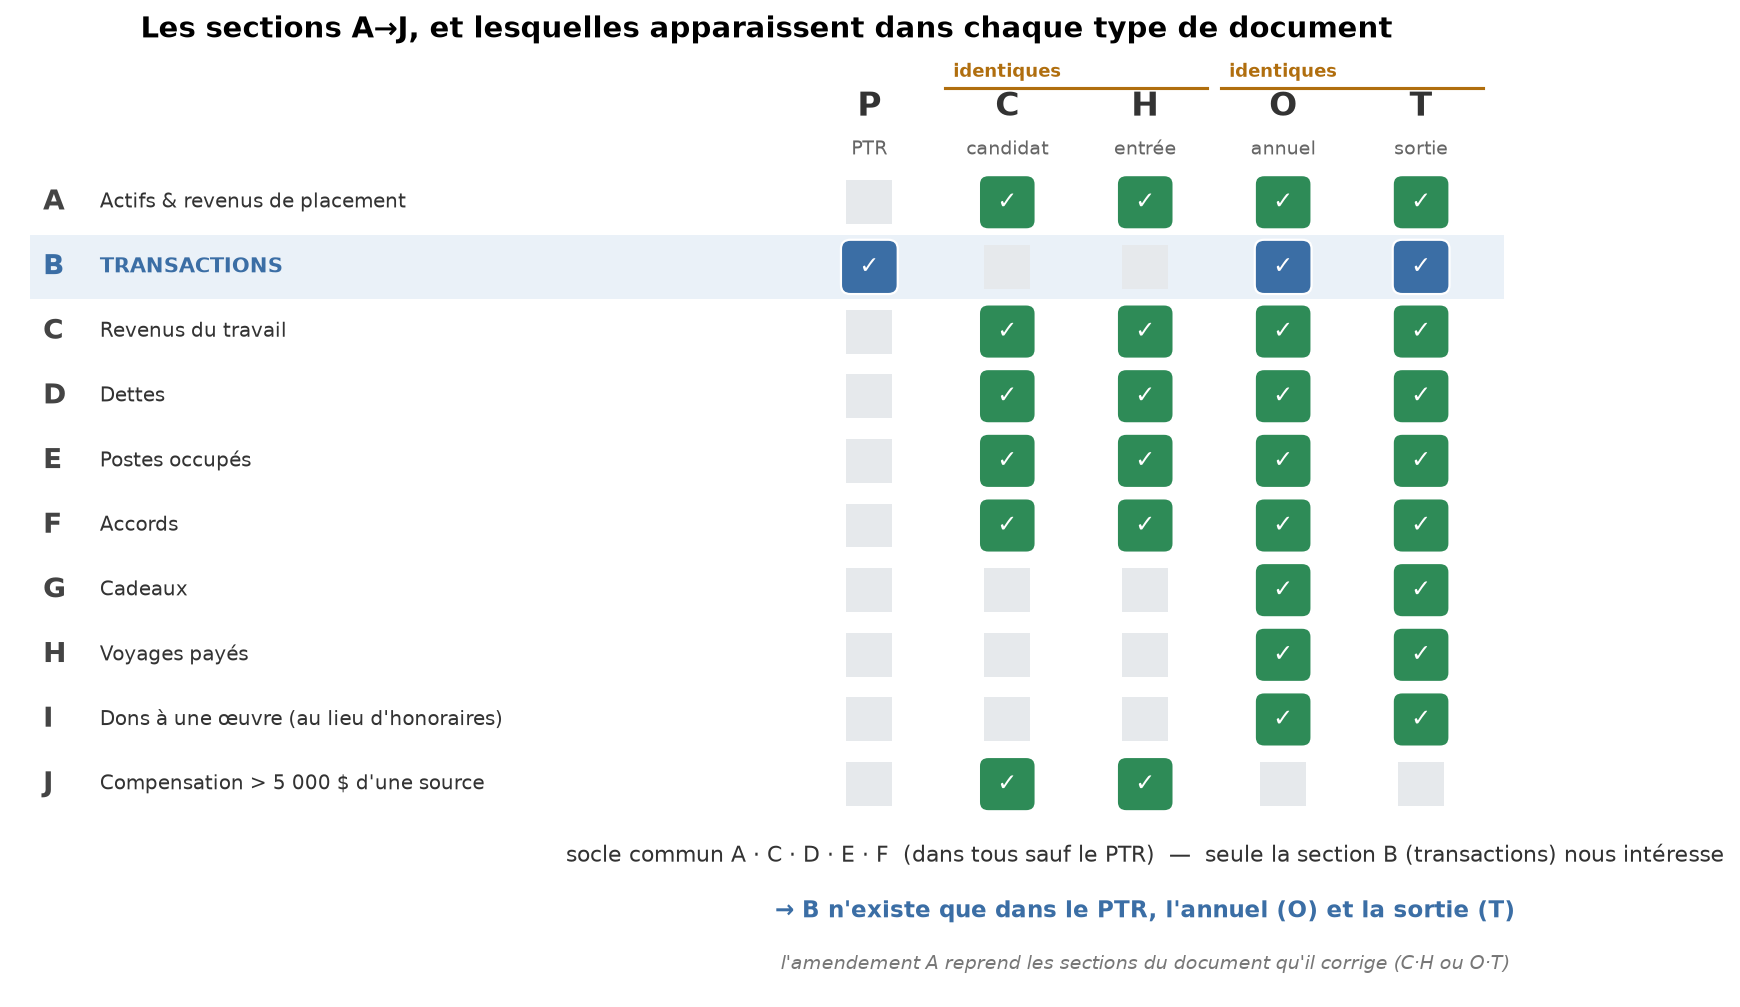
\includegraphics[height=0.54\textheight]{png/figs_deck/fig_sections_matrix.png}\\[0.5mm]
  {\footnotesize seules \textbf{deux} nous servent : la \textbf{\co{B}} = les transactions (on trade ça) ;
   la \textbf{\co{A}} (patrimoine) sert à \emph{vérifier} --- le reste est un socle commun}
\end{frame}

% ── III.4 · Le patrimoine : le stock (Schedule A) ───────────────────────
\begin{frame}{2 · Le patrimoine --- la matière première}
  \begin{columns}[c]
    \begin{column}{0.5\textwidth}
      \colorbox{dataC!12}{\parbox{0.95\linewidth}{\footnotesize\vspace{0.6mm}
        \textbf{Schedule A --- le patrimoine déclaré}\\[0.6mm]
        {\Large\textbf{420\,916}} lignes élec \textbf{+ 188\,970} papier OCR\\
        {\scriptsize les « photos » d'entrée, annuelles et de sortie}\vspace{0.6mm}}}\\[3mm]
      {\footnotesize\color{black!70} les rapports \co{O}/\co{A}/\co{T} ajoutent aussi des
       \textbf{mouvements datés} (surtout fonds \& ETF), superposés entre les photos}
    \end{column}
    \begin{column}{0.48\textwidth}
      {\footnotesize Ce n'est pas un \emph{signal} (trop tardif), mais c'est la
       \textbf{matière première} qui manquait :}\\[2mm]
      \choixbox{le \textbf{stock} détenu à chaque instant. Avec lui, on peut
       \textbf{reconstruire le portefeuille daté} de chaque membre --- et le
       \textbf{vérifier}.}\\[2mm]
      {\scriptsize\color{black!60} rappel : le \textbf{signal} daté au trade reste les
       \textbf{161\,076} transactions PTR (Partie I)}
    \end{column}
  \end{columns}
\end{frame}

% ── III.5 · Deux compteurs ───────────────────────────────────────────────
\begin{frame}{3 · Reconstruire --- deux compteurs : 822 $\neq$ 56}
  \begin{columns}[c]
    \begin{column}{0.48\textwidth}\centering
      \colorbox{helec!12}{\parbox{0.94\linewidth}{\centering\footnotesize\vspace{0.6mm}
        \textbf{RECONSTRUIRE}\\{\scriptsize le portefeuille daté de \emph{chaque} membre}\\[1mm]
        {\Huge\textbf{822}}\\{\scriptsize membres à $\geq$ 2 photos datées}\vspace{0.6mm}}}
    \end{column}
    \begin{column}{0.48\textwidth}\centering
      \colorbox{okgreen!18}{\parbox{0.94\linewidth}{\centering\footnotesize\vspace{0.6mm}
        \textbf{VÉRIFIER}\\{\scriptsize l'identité entrée\,+\,flux\,$\supseteq$\,sortie}\\[1mm]
        {\Huge\textbf{56}}\\{\scriptsize cycles complets, testables des deux côtés}\vspace{0.6mm}}}
    \end{column}
  \end{columns}
  \vspace{2.5mm}
  {\footnotesize pourquoi si différents ? \textbf{vérifier} exige les \textbf{deux} photos
   (entrée \emph{et} sortie) \textbf{et} des actions cotées des deux côtés --- rare. Ce sont
   \textbf{deux périmètres distincts} : reconstruire ($\geq$ 2 photos) $\neq$ vérifier
   (cycle complet testable, détaillé au \textbf{§4}).}\\[1.5mm]
  {\scriptsize\color{black!60} fil rouge : \textbf{Dean Phillips} (Minnesota, entré 2019) fait
   partie des \textbf{56} --- on le suivra jusqu'au bout}
\end{frame}

% ── III.6 · La photo de départ ───────────────────────────────────────────
\begin{frame}{3 · Reconstruire --- la photo d'ancrage : 284 = 252 + 32}
  \centering
  \begin{tikzpicture}[node distance=6mm]
    \node[step=helec, text width=3.2cm, minimum height=1.5cm, font=\footnotesize] (h)
      {\textbf{\large 252}\\{\scriptsize par un \co{H}\\(New Filer)}};
    \node[step=dataC, text width=3.2cm, minimum height=1.5cm, font=\footnotesize, right=of h] (c)
      {\textbf{\large 32}\\{\scriptsize par la \textbf{porte \co{C}}\\(3 garde-fous)}};
    \node[step=okgreen, text width=3.2cm, minimum height=1.5cm, font=\footnotesize, right=of c] (t)
      {\textbf{\large 284}\\{\scriptsize membres \textbf{ancrés}}};
    \node[step=grisC, text width=3.2cm, minimum height=1.5cm, font=\footnotesize, right=of t] (z)
      {\textbf{\large 616}\\{\scriptsize sans photo d'entrée}};
    \draw[arr] (h) -- (c); \draw[arr] (c) -- (t);
  \end{tikzpicture}\\[3mm]
  {\footnotesize \textbf{284 + 616 = 900}. La \textbf{porte \co{C}} récupère 32 candidats devenus
   élus, sous 3 garde-fous : dépôt \textbf{électronique}, \textbf{tickérisé}, déposé \textbf{$\leq$ 1 an}
   avant la prise de poste (sinon c'est une photo de réélection, pas d'entrée).}\\[1.5mm]
  {\scriptsize\color{black!60} Dean Phillips : photo d'entrée déposée à son arrivée en \textbf{2019}}
\end{frame}

% ── III.7 · Le moteur ────────────────────────────────────────────────────
\begin{frame}{3 · Reconstruire --- le moteur : 822 portefeuilles datés}
  \centering
  \begin{tikzpicture}[node distance=8mm]
    \node[step=helec, text width=3.4cm, minimum height=1.5cm, font=\footnotesize] (a)
      {\textbf{Ancrer}\\{\scriptsize sur la photo d'entrée}};
    \node[step=dataC, text width=3.4cm, minimum height=1.5cm, font=\footnotesize, right=of a] (b)
      {\textbf{Appliquer}\\{\scriptsize les flux datés\\(PTR + O/A/T)}};
    \node[step=okgreen, text width=3.4cm, minimum height=1.5cm, font=\footnotesize, right=of b] (c)
      {\textbf{Recaler}\\{\scriptsize à chaque nouvelle photo\\(le document fait foi)}};
    \draw[arr] (a) -- (b); \draw[arr] (b) -- (c);
  \end{tikzpicture}\\[3mm]
  {\footnotesize d'une photo à la suivante, \textbf{66,7\,\%} des positions sont directement
   \textbf{confirmées} :}\\[1.5mm]
  \choixbox{le patrimoine déclaré est en réalité \textbf{très stable}. Le « churn » apparent
   venait des \textbf{noms} de lignes qui changent, pas des positions.}
\end{frame}

% ── III.8 · Le test (équation) --- CONSERVÉ ──────────────────────────────
\begin{frame}{4 · Vérifier --- le test : la sortie dans l'entrée + les achats}
  \hfill{\scriptsize\color{black!55} Chambre uniquement ($\sim$90\,\% du corpus)}\\[1mm]
  \centering
  {\footnotesize \textbf{photo} = le patrimoine déclaré (Schedule A, aux entrées/sorties) ·
   \textbf{flux} = nos transactions --- l'équation \textbf{H\,+\,$\Sigma$P\,$\supseteq$\,T} ne se
   teste que si l'on a \textbf{les deux photos} :}\\[3mm]
  \resizebox{0.97\textwidth}{!}{%
  \begin{tikzpicture}[node distance=7mm]
    \node[step=grisC, text width=3.1cm, minimum height=1.4cm, font=\footnotesize] (a)
      {\textbf{\large 900}\\{\scriptsize membres passés par la Chambre 2014--2026}};
    \node[step=dataC, text width=3.1cm, minimum height=1.4cm, font=\footnotesize, right=of a] (b)
      {\textbf{\large 149}\\{\scriptsize entrés PUIS sortis\\(cycle complet)}};
    \node[step=helec, text width=3.1cm, minimum height=1.4cm, font=\footnotesize, right=of b] (c)
      {\textbf{\large 106}\\{\scriptsize les DEUX photos réellement déposées}};
    \node[step=okgreen, text width=3.1cm, minimum height=1.4cm, font=\footnotesize, right=of c] (d)
      {\textbf{\large 56}\\{\scriptsize actions cotées des deux côtés → \textbf{testables}}};
    \draw[arr] (a) -- (b); \draw[arr] (b) -- (c); \draw[arr] (c) -- (d);
  \end{tikzpicture}}\\[3mm]
  {\footnotesize la loi elle-même limite l'échantillon : \textbf{439} étaient déjà en
   poste en 2014 (pas de photo d'entrée), \textbf{437} sont encore en poste (pas de
   photo de sortie) ; la moitié des 106 ne détient \textbf{aucune action cotée}}\\[1.5mm]
  {\scriptsize\color{black!55} c'est \textbf{la même population de 900}, découpée ici
   \textbf{par testabilité} --- on la reverra découpée \emph{par force de preuve} (le bilan)}
\end{frame}

% ── III.9 · Le résultat --- CONSERVÉ ─────────────────────────────────────
\begin{frame}{4 · Vérifier --- le résultat : 87,8\,\% expliquées, 3,3\,\% non}
  \hfill{\scriptsize\color{black!55} Chambre uniquement}\\[0.3mm]
  \begin{columns}[c]
    \begin{column}{0.44\textwidth}\centering
      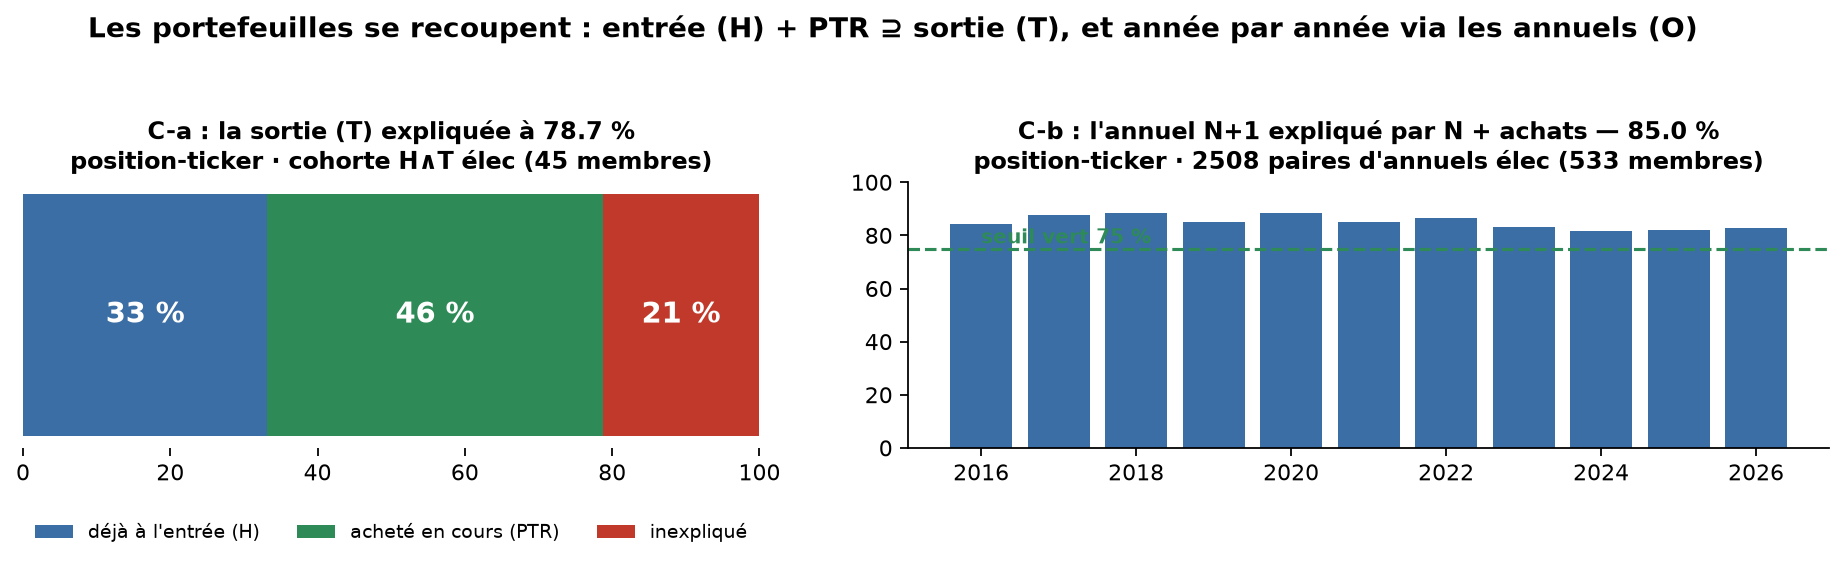
\includegraphics[width=\linewidth,height=0.42\textheight,keepaspectratio]{png/figs_deck/fig_v1_coherence.png}\\[0.5mm]
      {\scriptsize\color{black!60} premier passage : entrée + achats PTR expliquent
       \textbf{78,7\,\%} des \textbf{1\,371} positions de sortie de la \textbf{cohorte
       électronique} (H \emph{et} T déposés) → \textbf{292} inexpliquées}
    \end{column}
    \begin{column}{0.54\textwidth}
      \centering
      \begin{tikzpicture}[node distance=2mm]
        \node[bande=grisC, text width=6.6cm] (a) {\textbf{292 positions inexpliquées} \mbox{(21,3\,\%)} --- instruites \textbf{une par une} :};
        \node[bande=helec, text width=6.6cm, below=of a] (b)
          {\textbf{−125 déclarées AILLEURS} (annuels, sorties, PTR papier)\\
           {\tiny le taux monte : 78,7 → \textbf{87,8\,\%}}};
        \node[bande=dataC, text width=6.6cm, below=of b] (c)
          {\textbf{−122 structurelles} (comptes gérés, petites lignes, ETF exemptés)};
        \node[rectangle, rounded corners=2pt, draw=alertred, fill=alertred, line width=0.8pt,
              align=center, font=\scriptsize, text width=6.6cm, minimum height=0.62cm, below=of c] (d)
          {\color{white}\textbf{45 positions} vraiment inexpliquées = 3,3\,\% (14 membres)};
        \draw[arr] (a) -- (b); \draw[arr] (b) -- (c); \draw[arr] (c) -- (d);
      \end{tikzpicture}\\[0.6mm]
      \choixbox{chaque position inexpliquée est \textbf{classée par preuve documentaire}
       (table nominative conservée), pas éliminée statistiquement.}\\[0.6mm]
      {\scriptsize\color{black!55} −125 = 74 annuels + 49 sorties + 2 PTR papier ·
       −122 = 59 gérés + 32 $\leq$ 15\,k\$ + 30 ETF + 1 renommage}
    \end{column}
  \end{columns}
\end{frame}

% ── III.10 · Les cas ─────────────────────────────────────────────────────
\begin{frame}{4 · Vérifier --- deux cas qui éclairent}
  \begin{columns}[c]
    \begin{column}{0.5\textwidth}
      \colorbox{alertred!10}{\parbox{0.95\linewidth}{\footnotesize\raggedright\vspace{0.6mm}
        \textbf{\textcolor{alertred}{Le blind trust}} --- Dean Phillips sort en \textbf{2025} :
        \textbf{la totalité de ses titres cotés} devient \textbf{1 seule ligne} opaque
        (« Qualified Blind Trust »).\\[1mm]
        C'est une \textbf{disparition de couverture}, \emph{pas} un écart de conservation :
        la fiducie n'est plus dirigée par l'élu.\vspace{0.6mm}}}\\[2mm]
      {\scriptsize\color{black!60} 23 dépôts \co{B}, 5 élus ; Tom Malinowski (34 → 0) quitte
       ainsi la cohorte des testables}
    \end{column}
    \begin{column}{0.48\textwidth}\centering
      \fcolorbox{black!25}{white}{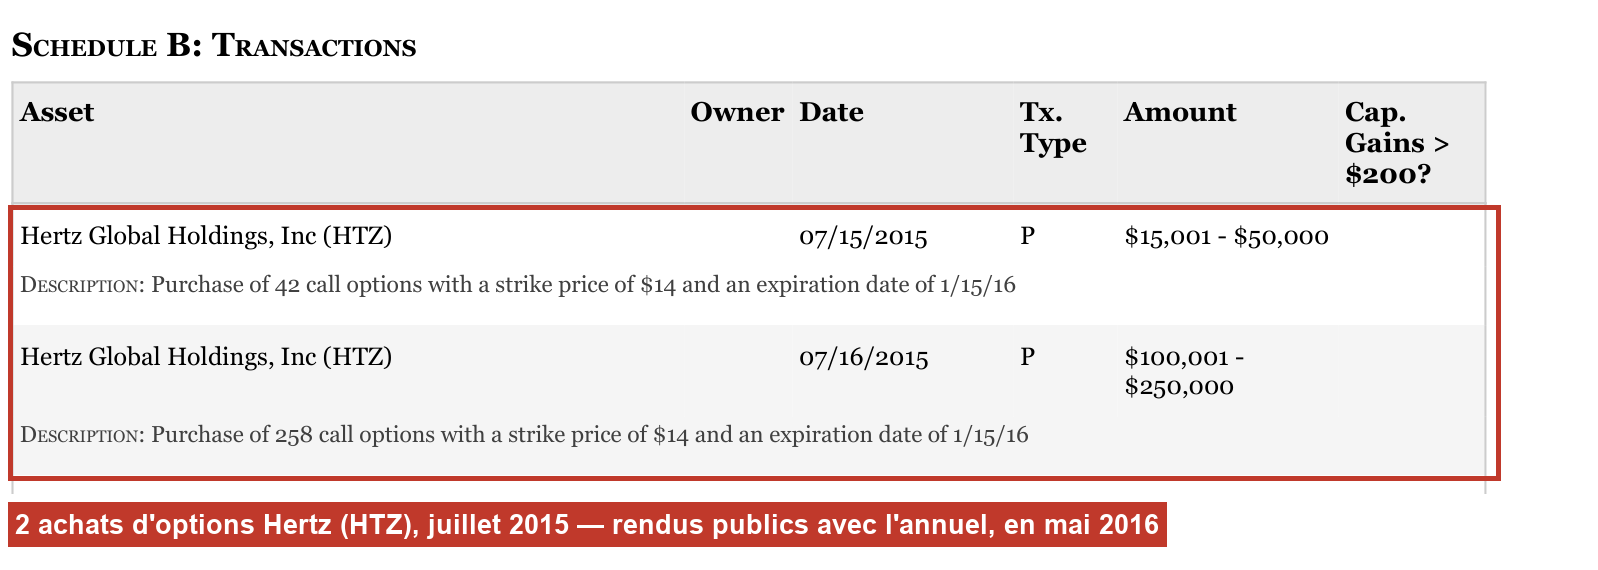
\includegraphics[width=0.9\linewidth,height=34mm,keepaspectratio]{png/figs_deck/fig_pelosi_schedb.png}}\\[1mm]
      {\footnotesize\textbf{La répétition} --- un amendement \co{A} re-déclare les trades
       de l'annuel qu'il corrige}\\[1mm]
      {\scriptsize\color{black!60} Pelosi 2014 : le même trade \textbf{3 fois} (\co{O}+\co{A}+\co{A})
       → dédoublonné par la clé naturelle}
    \end{column}
  \end{columns}
\end{frame}

% ── III.11 · Le bilan (registre) --- CONSERVÉ ────────────────────────────
\begin{frame}{4 · Vérifier --- le bilan : un statut par membre}
  \hfill{\scriptsize\color{black!55} Chambre uniquement}\\[1mm]
  \centering
  {\footnotesize chacun des \textbf{900} membres reçoit \textbf{un seul statut} --- du
   moins au plus exigeant :}\\[1mm]
  \begin{tikzpicture}[node distance=2mm]
    \node[rectangle, rounded corners=2pt, draw=grisC, fill=grisC!10, line width=0.8pt,
          text width=12.4cm, align=left, font=\scriptsize, inner sep=4.5pt] (r1)
      {\makebox[0.85cm][r]{\normalsize\textbf{20}}\;\; \textbf{hors d'atteinte} --- rien d'exploitable
       (patrimoine 100\,\% non coté, blind trust)};
    \node[rectangle, rounded corners=2pt, draw=dataC, fill=dataC!10, line width=0.8pt,
          text width=12.4cm, align=left, font=\scriptsize, inner sep=4.5pt, below=of r1] (r2)
      {\makebox[0.85cm][r]{\normalsize\textbf{715}}\;\; \textbf{reconstructible partiel} --- au moins
       une photo \textbf{ou} des transactions → des \textbf{morceaux datés}};
    \node[rectangle, rounded corners=2pt, draw=helec, fill=helec!10, line width=0.8pt,
          text width=12.4cm, align=left, font=\scriptsize, inner sep=4.5pt, below=of r2] (r3)
      {\makebox[0.85cm][r]{\normalsize\textbf{109}}\;\; \textbf{reconstructible complet} --- série
       datée de bout en bout\ldots{} mais pas de photo de \textbf{sortie} : \textbf{non testable}};
    \node[rectangle, rounded corners=2pt, draw=okgreen, fill=okgreen, line width=0.8pt,
          text width=12.4cm, align=left, font=\scriptsize, inner sep=4.5pt, below=of r3] (r4)
      {\color{white}\makebox[0.85cm][r]{\normalsize\textbf{56}}\;\; \textbf{vérifiable strict} ---
       les \textbf{deux} photos + actions cotées → l'équation \textbf{réellement testée}
       (le 87,8\,\% mesuré sur le sous-ensemble \textbf{électronique}) --- \emph{dont Dean Phillips}};
  \end{tikzpicture}\\[1.5mm]
  {\scriptsize\color{black!60} 20 + 715 + 109 + 56 = \textbf{900} --- une partition, rien ne se recouvre ·
   \textbf{autre découpage} des mêmes 900, cette fois \emph{par force de preuve} (et non par nombre de photos comme les 822)}\\[1.5mm]
  \choixbox{on affiche le \textbf{périmètre réel du test} (56 membres) plutôt que de
   laisser croire à une vérification universelle --- $\sim$9 reconstruits sur 10 restent
   \textbf{sans preuve}.}
\end{frame}

% ── III.12 · Teaser ──────────────────────────────────────────────────────
\begin{frame}{La suite --- à quoi sert ce patrimoine}
  \begin{columns}[c]
    \begin{column}{0.52\textwidth}
      {\footnotesize Un backtest qui part de \textbf{zéro} ignore le tiers « déjà là, jamais
       tradé » (les \textbf{33,2\,\%} du début).}\\[2.5mm]
      \choixbox{en \textbf{initialisant} chaque portefeuille à sa \textbf{photo d'entrée}
       plutôt qu'à zéro, on rend visible tout le patrimoine dès le départ.}\\[2.5mm]
      {\footnotesize c'est la piste du \textbf{backtest « adapté »} --- une direction de
       recherche ouverte, à explorer séparément.}
    \end{column}
    \begin{column}{0.46\textwidth}\centering
      \begin{tikzpicture}[node distance=5mm]
        \node[bande=grisC, text width=5.0cm] (a) {backtest \textbf{à zéro}\\{\scriptsize un tiers du patrimoine manque}};
        \node[bande=okgreen, text width=5.0cm, below=of a] (b) {backtest \textbf{ancré à l'entrée}\\{\scriptsize le patrimoine complet, dès J0}};
        \draw[arr] (a) -- (b);
      \end{tikzpicture}\\[2mm]
      {\scriptsize\color{black!55} sans nouveau chiffre ici : le verdict du backtest adapté
       ne fait pas partie de la couche \emph{données}}
    \end{column}
  \end{columns}
\end{frame}

\section{Annexes}

\begin{frame}[plain]
  \centering\vfill
  {\color{helec!85}\large\textbf{Annexes}}\\[2mm]
  {\color{black!88}\fontsize{29}{33}\selectfont\textbf{La réserve pour questions}}\\[4mm]
  {\color{helec!45}\rule{0.30\textwidth}{1.2pt}}\\[4mm]
  {\color{black!55}\large A1--A7 : documents exemples · détails des cascades · cas particuliers}
  \vfill
\end{frame}

% ── A1 · Le PTR lisible en grand ──
\begin{frame}{A1 --- Le document lisible : un PTR électronique}
  \begin{columns}[T]
    \begin{column}{0.55\textwidth}\centering
      \fcolorbox{helec}{white}{\clickzoom{fig_ptr_digital}{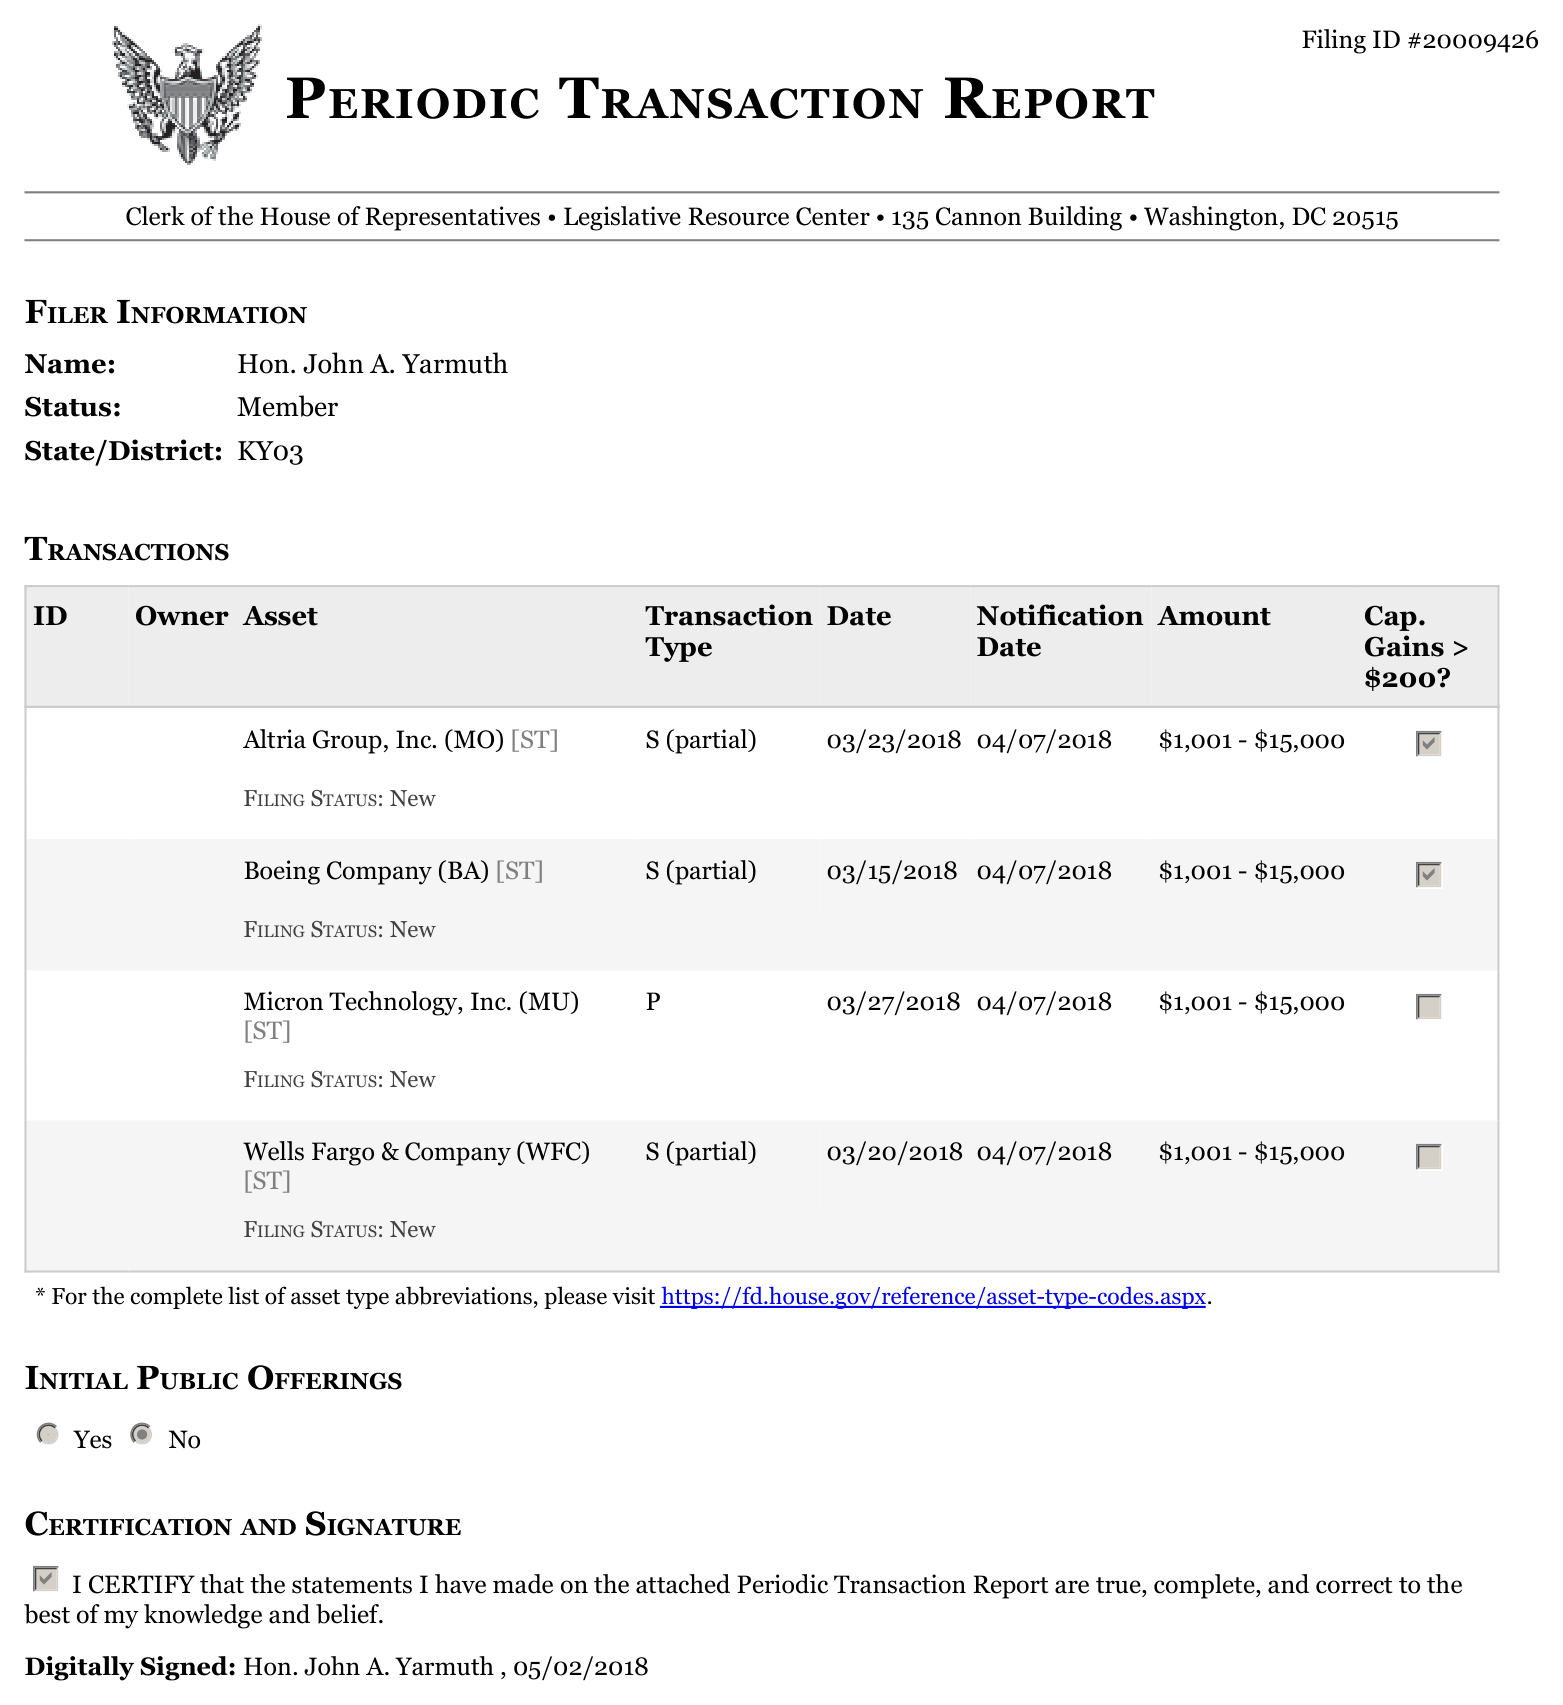
\includegraphics[width=0.92\linewidth,height=64mm,keepaspectratio]{png/figs_deck/fig_ptr_digital.png}}}\\[0.5mm]
      {\scriptsize\color{black!60} PTR électronique complet (Hon.\ John A.\ Yarmuth, KY03)}
    \end{column}
    \begin{column}{0.43\textwidth}
      {\footnotesize
      · un PDF \textbf{lisible par machine} (couche texte)\\[1.5mm]
      · le ticker est imprimé \textbf{entre parenthèses} : \co{(BA)},
        le type d'actif entre crochets : \co{[ST]}\\[1.5mm]
      · deux dates par ligne (trade / notification --- cette dernière est jetée)
        + fourchette de montant\\[1.5mm]
      · \textbf{7\,996} lignes au montant coupé en deux, recollées avant lecture}
    \end{column}
  \end{columns}
\end{frame}

% ── A2 · La liste eFD, en détail ──
\begin{frame}{A2 --- Le portail du Sénat : ce que rend la recherche}
  \centering
  \fcolorbox{black!25}{white}{\clickzoom{site_senate_results}{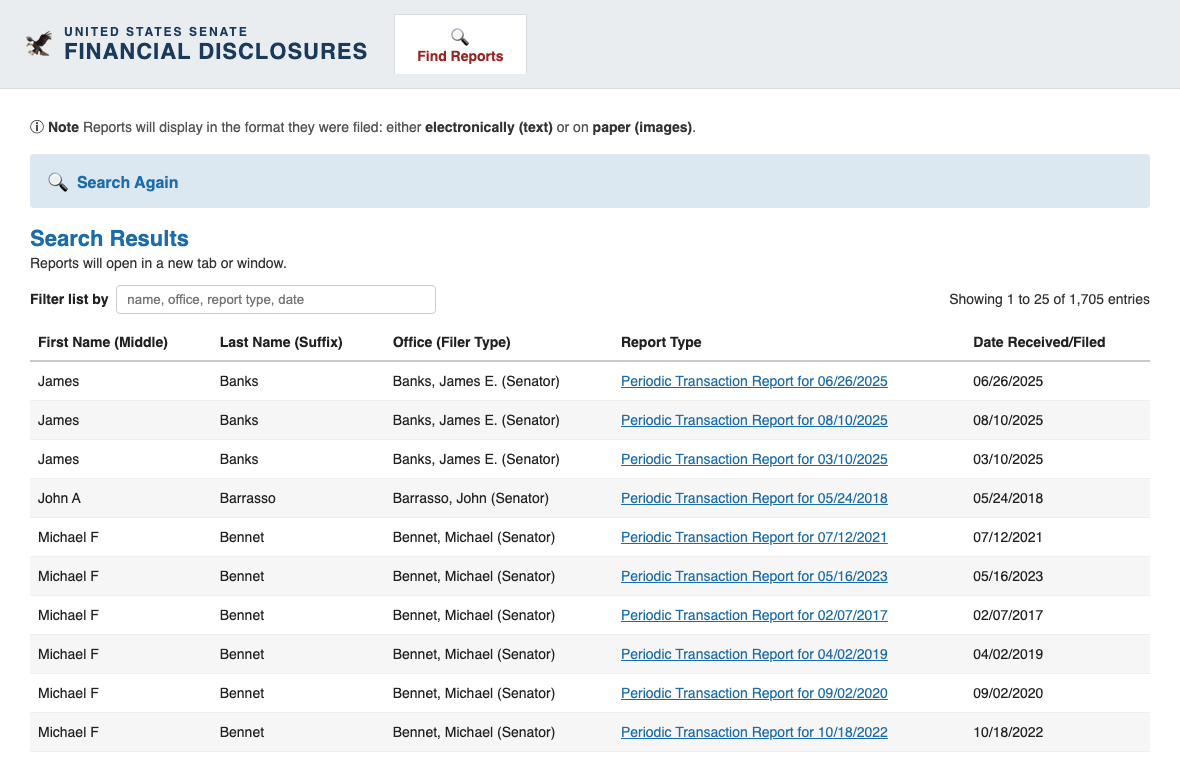
\includegraphics[width=0.78\textwidth,height=0.60\textheight,keepaspectratio]{png/figs_deck/site_senate_results.png}}}\\[1.5mm]
  {\footnotesize la liste réelle des dépôts (1b) --- \textbf{un lien par dépôt} :
   chacun s'ouvre en \textbf{page web} ou en \textbf{papier scanné}, c'est là que se décide la
   voie d'extraction}\\[1mm]
  {\scriptsize\color{black!60} les PTR sont \textbf{un type parmi d'autres} au Sénat
   aussi (annuels, extensions, \emph{blind trusts}…) --- on ne demande que les PTR}
\end{frame}

% ── A3 · La matrice des sections ──
\begin{frame}{A3 --- Le même formulaire, des sections en commun}
  \centering
  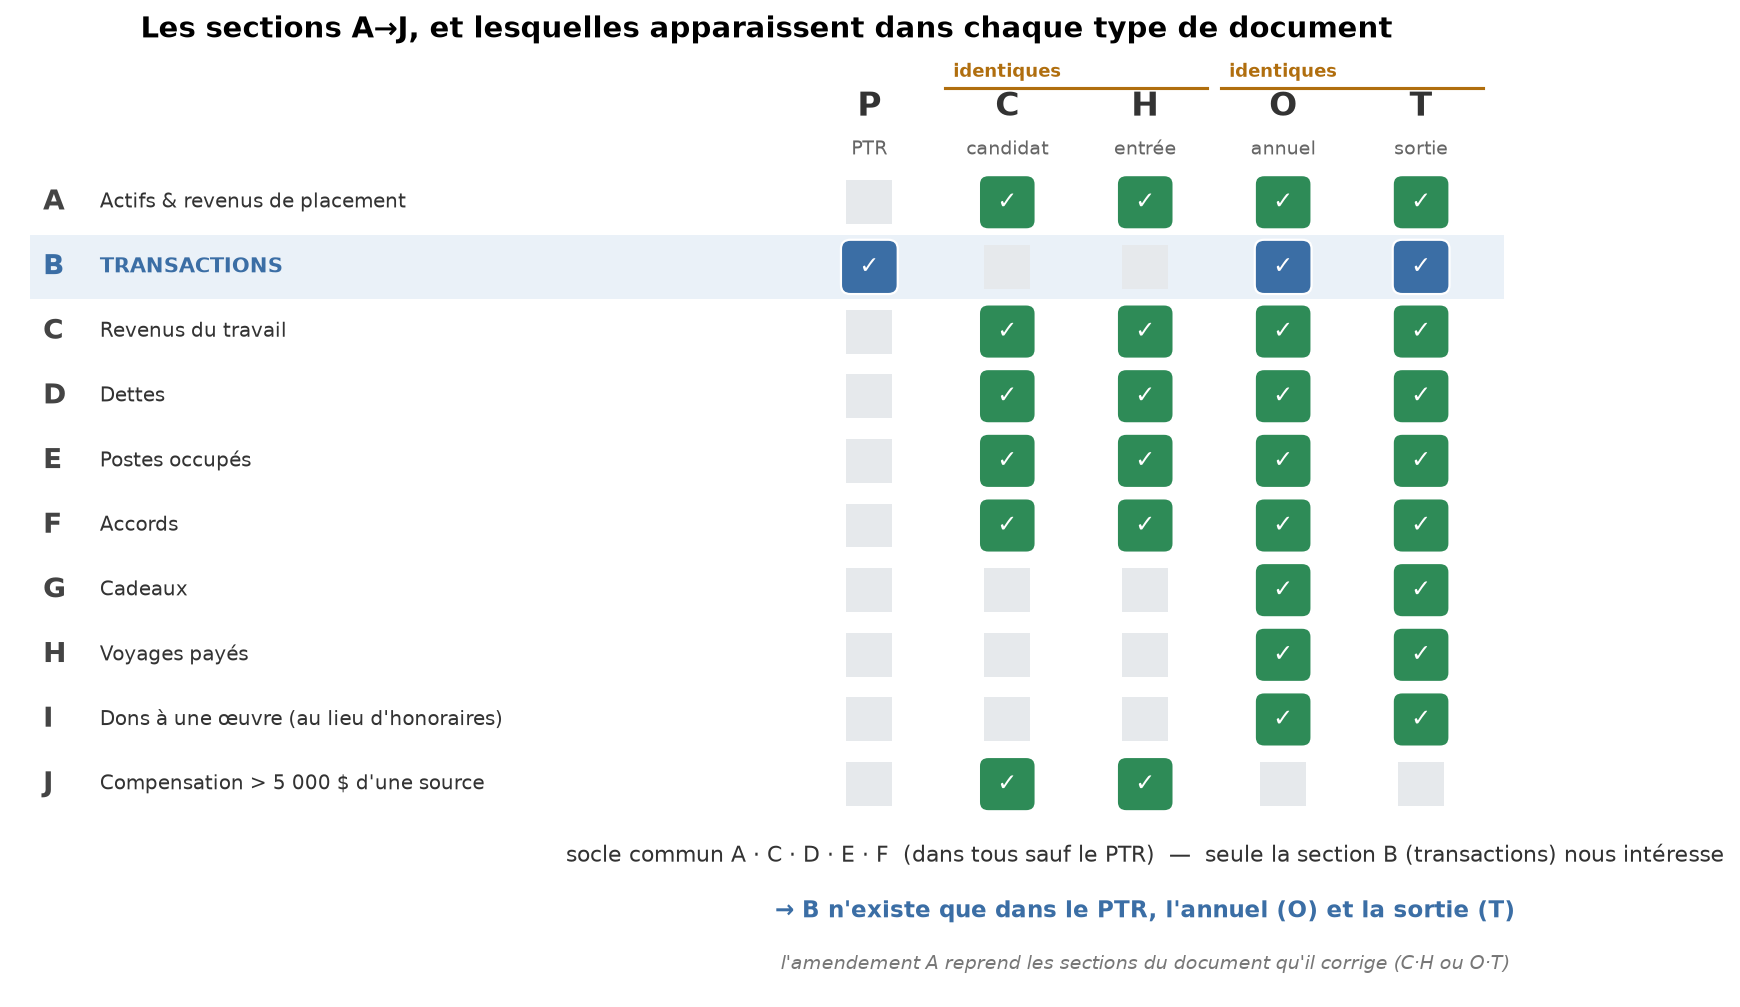
\includegraphics[height=0.61\textheight]{png/figs_deck/fig_sections_matrix.png}\\[0.5mm]
  {\footnotesize la \textbf{section B} = les transactions ; le reste est un socle
   commun, la \textbf{A} (patrimoine) sert à \emph{vérifier}}
\end{frame}

% ── A6 · Les dates arbitrées au PDF ──
\begin{frame}{A6 --- Qui a raison sur les dates ? Le PDF officiel arbitre toujours}
  \centering
  {\footnotesize pour un même (élu, ticker, sens), quand notre date et celle de Quiver
   divergent dans un même dépôt, \textbf{545 candidats} méritent l'œil → on
   \textbf{rouvre le PDF} :}\\[2mm]
  {\footnotesize
  \begin{tabular}{@{}>{\raggedright\arraybackslash}p{0.34\linewidth}>{\raggedright\arraybackslash}p{0.24\linewidth}>{\raggedright\arraybackslash}p{0.30\linewidth}@{}}
    \toprule
    \textbf{le PDF montre…} & \textbf{exemple réel} & \textbf{traitement} \\
    \midrule
    coquille du déposant, prouvable & \ttfamily 3031-04-30 & corrigée → 2021 \\[0.6mm]
    coquille littérale & \ttfamily 01/35/22 & \textcolor{okgreen}{\textbf{transcrite telle quelle}} \\[0.6mm]
    notre OCR s'est trompé & Khanna/COST \ttfamily 09-31 & re-lue au PDF → \ttfamily 08-16 \\[0.6mm]
    désaccord Quiver & McCaul/GOOGL $\Delta$11 j & arbitré au PDF \\
    \bottomrule
  \end{tabular}}\\[2.5mm]
  {\scriptsize\color{black!60} principe : le \textbf{PDF officiel} arbitre toujours ---
   on reste fidèle à la source, même à ses coquilles littérales}
\end{frame}

% ── A7 · Détails ──
\begin{frame}{A7 --- Détails : la couverture des entrées/sorties, les pièges d'identité}
  \begin{columns}[T]
    \begin{column}{0.48\textwidth}\footnotesize
      \textbf{couverture des entrées/sorties (Chambre)} :\\[1mm]
      {\scriptsize
      \begin{tabular}{@{}p{0.30\linewidth} p{0.60\linewidth}@{}}
        \toprule
        \textbf{470 entrées} depuis 2014 & 82\,\% ont déposé un \textbf{H} (photo
          d'entrée) · 16\,\% un \textbf{C} à la place → \textbf{98\,\% couverts} \\
        \midrule
        \textbf{463 sorties} définitives & 81\,\% ont déposé un \textbf{T} (photo de
          sortie) ; les 86 sans T : partis au Sénat/exécutif (dispensés), décès \\
        \bottomrule
      \end{tabular}}\\[1.5mm]
      {\scriptsize la photo d'entrée : \textbf{252} ancrés par un H · \textbf{32} par
       un C = \textbf{284} portefeuilles d'entrée datés}
    \end{column}
    \begin{column}{0.48\textwidth}\footnotesize
      \textbf{pièges d'identité réels, réparés} (3) :\\[1mm]
      {\scriptsize
      · l'homonyme \textbf{Bob Casey} (\co{C000228} → \co{C001070}) : deux vraies
        personnes --- un représentant du Texas, un sénateur de Pennsylvanie\\[1mm]
      · \textbf{42 lignes d'Angie Craig} sans identifiant, réparées à la lecture ---
        le fichier extrait, lui, reste figé}\\[3mm]
      \textbf{cascade secteur} (5) :\\[1mm]
      {\scriptsize yfinance (le secteur factuel) → LLM contraint GICS → overrides
       manuels pour les cas connus}
    \end{column}
  \end{columns}
\end{frame}

% ── A8 --- Le corpus extrait (déplacé de l'Extraction : présuppose l'identité (3) et la dédup (6)) ──
\begin{frame}{A8 --- Le corpus extrait : 170\,920 transactions --- dont $\sim$40\,\% de deux élus}
  \centering
  {\footnotesize les quatre voies réunies donnent \textbf{170\,920 transactions
   extraites} (2014--2026), ramenées à \textbf{169\,000 uniques} au dédoublonnage
   (6) --- et cette matière est \textbf{très déséquilibrée} :}\\[1.2mm]
  \begin{tikzpicture}
    \draw[fill=helec, draw=none] (0,0) rectangle (4.125,0.5);
    \draw[fill=hocr, draw=none] (4.125,0) rectangle (10.677,0.5);
    \draw[fill=selec, draw=none] (10.677,0) rectangle (11.717,0.5);
    \draw[fill=socr, draw=none] (11.717,0) rectangle (12.0,0.5);
    \node[font=\scriptsize, color=white] at (2.06,0.25) {\textbf{Chambre élec.\ 34,4\,\%}};
    \node[font=\scriptsize, color=black!75] at (7.40,0.25) {\textbf{Chambre OCR 54,6\,\%}};
    \node[font=\tiny, color=white] at (11.20,0.25) {\textbf{8,7}};
    \node[font=\tiny, color=black!75, above=1mm of {(11.86,0.5)}] {Sénat OCR 2,4\,\%};
  \end{tikzpicture}\\[2mm]
  \begin{columns}[T]
    \begin{column}{0.55\textwidth}\centering
      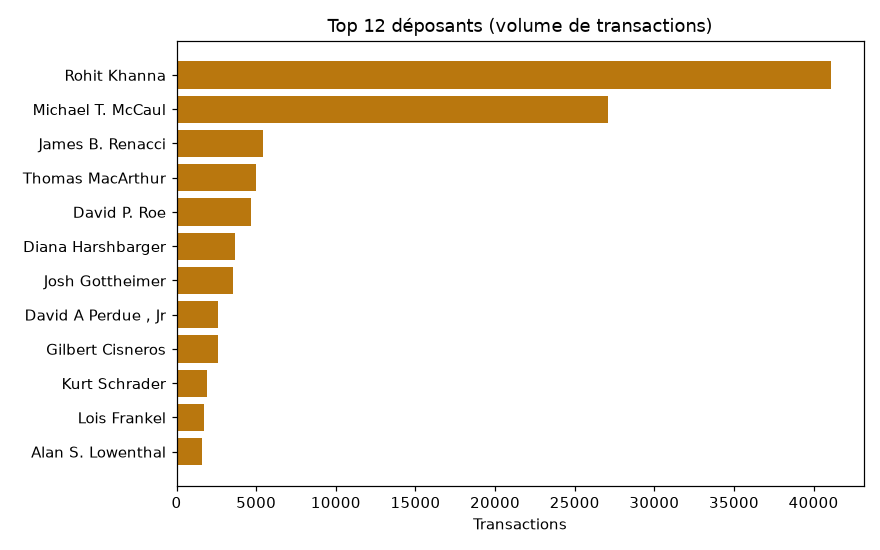
\includegraphics[width=0.74\linewidth]{png/quality/top_deposants.png}
    \end{column}
    \begin{column}{0.43\textwidth}
      \colorbox{warnorange!12}{\parbox{0.96\linewidth}{\footnotesize\vspace{0.5mm}
        \textbf{\textcolor{warnorange}{très concentré}} --- Khanna
        (\textbf{41\,080} txns) et McCaul (\textbf{27\,123}) pèsent à eux deux
        \textbf{$\sim$40\,\%} du corpus, et déclarent \textbf{exclusivement sur
        papier} (\mbox{100\,\%} OCR)\vspace{0.5mm}}}\\[1.5mm]
      {\footnotesize le papier n'est pas un détail : c'est \textbf{la majorité du
       corpus} --- d'où l'effort d'OCR de 2c et 2e}
    \end{column}
  \end{columns}
\end{frame}

% ════ ANNEXE BACKTEST — déplacée de la Partie II (sous le capot + tables) ════
\chapdivider{Annexe · Backtest}{Sous le capot}{le détail technique : shrinkage de $\Sigma$, et la contre-preuve membre par membre}

% ── An3 · Ledoit-Wolf (ex-S3-14) ──
\begin{frame}{Le shrinkage répare l'estimateur de $\Sigma$ — pas la stratégie}
  \centering
  {\footnotesize $\Sigma_{\text{shrink}}=\delta\,F+(1-\delta)\,\Sigma_{\text{emp}}$,\;
   $\delta=\frac{\pi-\rho}{T\gamma}$ borné à $[0,1]$ —
   3 cibles $F$ : diagonale (LW 2004) · single-factor (LW 2001) · corrélation constante (LW 2003)}\\[1mm]
  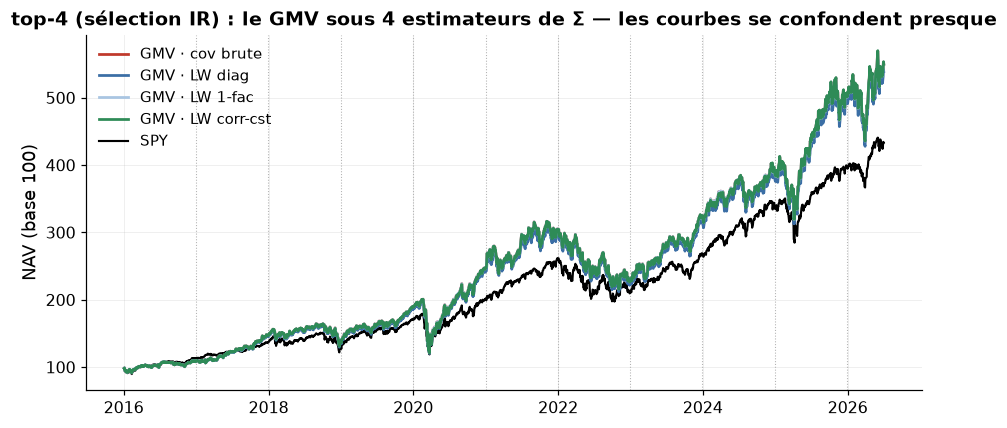
\includegraphics[height=0.40\textheight]{png/figs_deck/fig_05b_gmv_ledoitwolf.png}\\[1.5mm]
  \tuile{okgreen}{−4,5 → −4,3}{\%/an : l'artefact GMV\\(sél. appr) tempéré}\hfill
  \tuile{okgreen}{−2,76 → −2,46}{le t remonte…\\sans devenir positif}\hfill
  \tuile{helec}{50 → 25}{conditionnement\\de $\Sigma$ (LW diag)}\hfill
  \tuile{grisC}{0,67 → 0,55}{concentration HHI\\du panier GMV}\\[1.5mm]
  {\scriptsize\color{black!60} intensité mesurée $\delta_{\text{LW}} \approx 0{,}05$ —
   verdict invariant à l'estimateur : \textbf{$\beta$ de style $\approx$ 1,20, zéro $\alpha$}}
\end{frame}

% ── An4 · Contre-preuve IR ↔ β (ex-S3-8) ──
\begin{frame}{La contre-preuve point par point : la queue droite de l'IR, c'était du $\beta$}
  \centering
  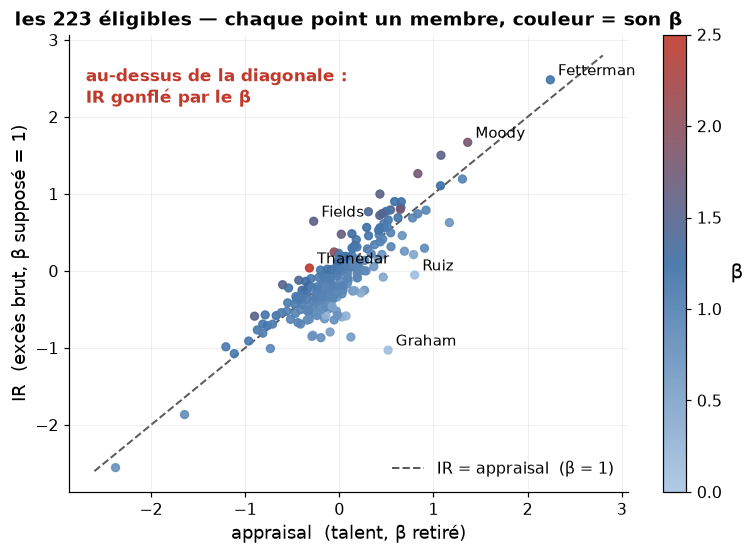
\includegraphics[height=0.63\textheight]{png/figs_deck/fig_05b_ir_vs_appraisal.png}\\[1mm]
  {\footnotesize au-dessus de la diagonale : classé par l'IR \textbf{grâce à son $\beta$} —
   l'ajustement dégonfle la queue droite}\\[0.8mm]
  {\scriptsize\color{black!60} c'est la version « membre par membre » du 20 → 12 :
   on juge chaque stratégie en excès brut \textbf{et} en $t_{\mathrm{appr}}$}
\end{frame}

% ══════════════════════════════════════════════════════════════════
% PARTIE III — TABLES DE DONNÉES  (notebook 09 : membres · tickers · panel)
% Figures : png/figs_deck/fig_09_*.png (régénérées du notebook, fidèles aux inline)
% ══════════════════════════════════════════════════════════════════
% ── Séparateur · PARTIE III ──

\chapdivider{Annexe · Backtest}{Tables membres, tickers, panel}{la donnée qui porte le backtest, membre par membre}


% ── T1 · Les 4 livrables ──
\begin{frame}{Quatre tables livrées — chaque colonne a une histoire}
  \centering
  \vspace{2mm}
  \tuile{dataC}{372 × 94}{\co{membres.csv}\\1 ligne = 1 élu}\hfill
  \tuile{dataC}{4\,618 × 40}{\co{tickers.csv}\\1 ligne = 1 titre}\hfill
  \tuile{dataC}{2\,628 × 11}{\co{membres\_annees.csv}\\1 ligne = (élu, année)}\hfill
  \tuile{grisC}{145}{colonnes documentées\\(le dictionnaire)}\\[7mm]
  {\footnotesize aucune stratégie ici : de la donnée \textbf{propre, comprise et auditable} —
   cette partie raconte l'histoire visuelle derrière ces colonnes, une figure par famille}
\end{frame}

% ── T2 · L'entonnoir ──
\begin{frame}{Rien n'entre dans les tables sans passer l'entonnoir}
  \centering
  \bmaths{deux portes : le trade exploitable, puis l'élu jugeable}%
    {\text{reconstruit}\iff r_m\ \text{calculable}\qquad
     \text{éligible}\iff n_{\text{trades}}\ge 10\ \text{et}\ n_{\text{jours}}\ge 126}
  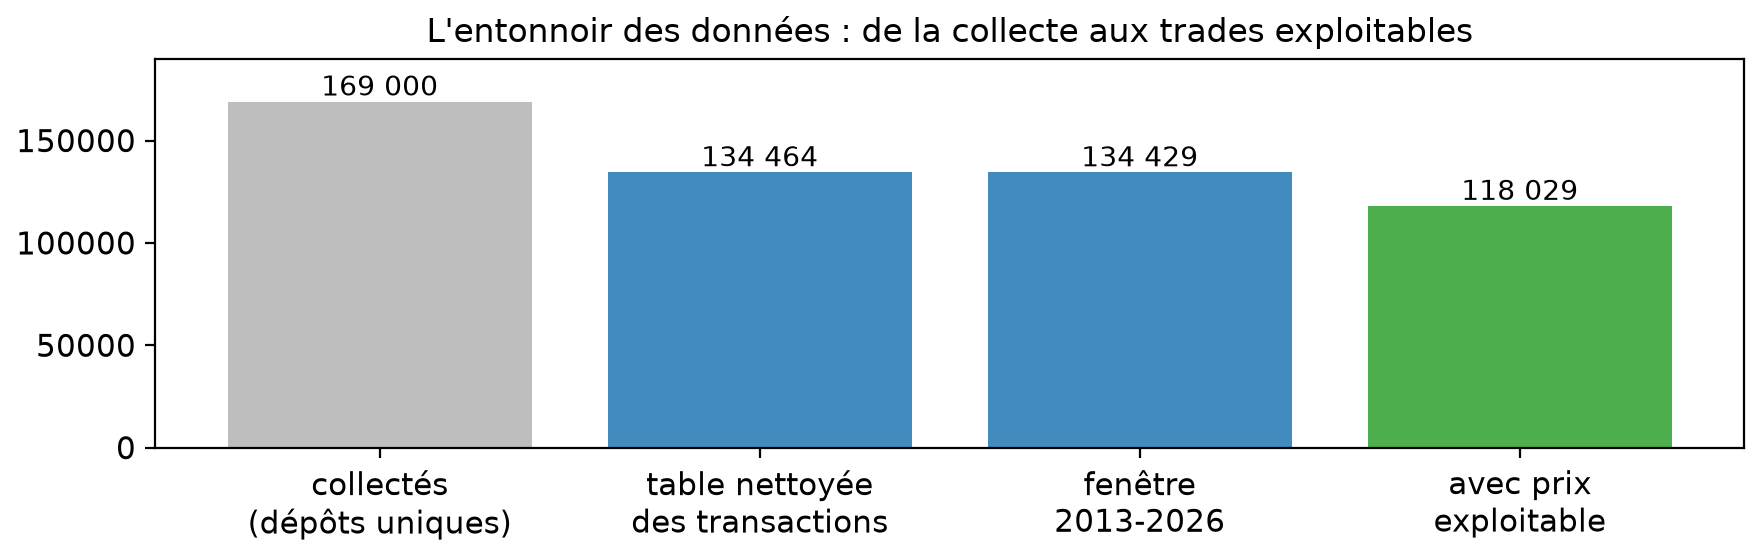
\includegraphics[width=0.80\textwidth,height=0.52\textheight,keepaspectratio]{png/figs_deck/fig_09_entonnoir.png}\\[2mm]
  {\footnotesize des 169\,000 dépôts bruts, seuls les trades à \textbf{prix exploitable} alimentent
   les quatre tables — et la chaîne des élus suit : 372 → 359 → 266 reconstruits → 223 éligibles}\\[1.5mm]
  \badge{helec}{118\,029 trades exploitables}\;
  \badge{helec}{223 élus éligibles}
\end{frame}

% ── T2bis · Le moteur : ce qu'on reconstruit ──
\begin{frame}{Ce qu'on reconstruit : du trade déclaré au portefeuille quotidien}
  \centering
  {\footnotesize chaque trade a \textbf{deux dates} : $\tau_j$ = \textbf{transaction} (reconstruit
   le portefeuille) ; $\delta_j$ = \textbf{divulgation} (la transparence) —
   $\mathrm{lag}_j=\delta_j-\tau_j$, loi $\le 45$ j}\\[3mm]
  \resizebox{0.98\textwidth}{!}{%
  \begin{tikzpicture}[node distance=6mm]
    \node[step=grisC, text width=4.0cm] (n1)
      {\textbf{LE TRADE}\\[1mm]
       $j=(m_j,\,k_j,\,d_j,\,\tau_j,\,\delta_j,\,A_j)$\\[0.8mm]
       {\tiny élu · titre · buy/sell · 2 dates ·\\montant (milieu de fourchette)}};
    \node[step=helec, text width=3.2cm, right=of n1] (n2)
      {\textbf{COMPTER (FIFO)}\\[1mm]
       $n_k^m(t)$ parts\\[0.8mm]
       {\tiny jamais négatif — on ne\\vend que ce qu'on détient}};
    \node[step=dataC, text width=3.8cm, right=of n2] (n3)
      {\textbf{VALORISER}\\[1mm]
       $V_m(t)=\sum_k n_k^m(t)\,P_k(t)$\\[0.8mm]
       {\tiny et les poids $w_k^m(t)$}};
    \node[step=okgreen, text width=4.7cm, right=of n3] (n4)
      {\textbf{MESURER} (time-weighted)\\[1mm]
       $r_m(t)=\dfrac{\sum_k n_k^m(t{-}1)\,P_k(t)}{\sum_k n_k^m(t{-}1)\,P_k(t{-}1)}-1$};
    \draw[arr] (n1) -- (n2); \draw[arr] (n2) -- (n3); \draw[arr] (n3) -- (n4);
  \end{tikzpicture}}\\[4mm]
  \badge{dataC}{tout \co{membres.csv} dérive de trois objets : $n_k^m(t)$ · $V_m(t)$ · $r_m(t)$}\\[1.2mm]
  {\scriptsize\color{black!55} le moteur de la Partie II, relu membre par membre —
   les 6 familles qui suivent en tirent chacune leurs colonnes}
\end{frame}

% ── T3 · La fiche (1/6) : identité ──
\begin{frame}{La fiche (1/6) — identité : chaque élu a la sienne, suivons-en une}
  \centering
  \bmaths{colonnes \co{comites} · \co{secteurs\_juridiction}}%
    {\mathrm{comites}(m)=\bigcup_{j}\mathrm{codes}_j\qquad
     \mathrm{secteurs\_juridiction}(m)=\bigcup_{c\,\in\,\mathrm{comites}(m)}\mathrm{COMITE\_GICS}[c]}
  
\includegraphics[width=0.78\textwidth,height=0.52\textheight,keepaspectratio]{png/figs_deck/fig_09_identite.png}\\[2mm]
  {\footnotesize 94 colonnes en \textbf{6 familles} (identité, activité, portefeuille, durées,
   risque-perf, comportement) ; pour les incarner, un fil rouge : Nancy Pelosi}\\[1.5mm]
  \badge{dataC}{372 fiches}\;
  \badge{dataC}{6 familles de colonnes}
\end{frame}

% ── T4 · La fiche (2/6) : activité ──
\begin{frame}{La fiche (2/6) — activité : tout tient en une figure}
  \centering
  \bmaths{colonnes \co{buy\_share} · \co{part\_late} (et \co{notional\_total}, \co{lag\_med})}%
    {\mathrm{buy\_share}=\frac{\#\{d_j=\mathrm{buy}\}}{\#j}\qquad
     \mathrm{part\_late}=\mathbb{P}(\delta_j-\tau_j>45\ \text{j})}
  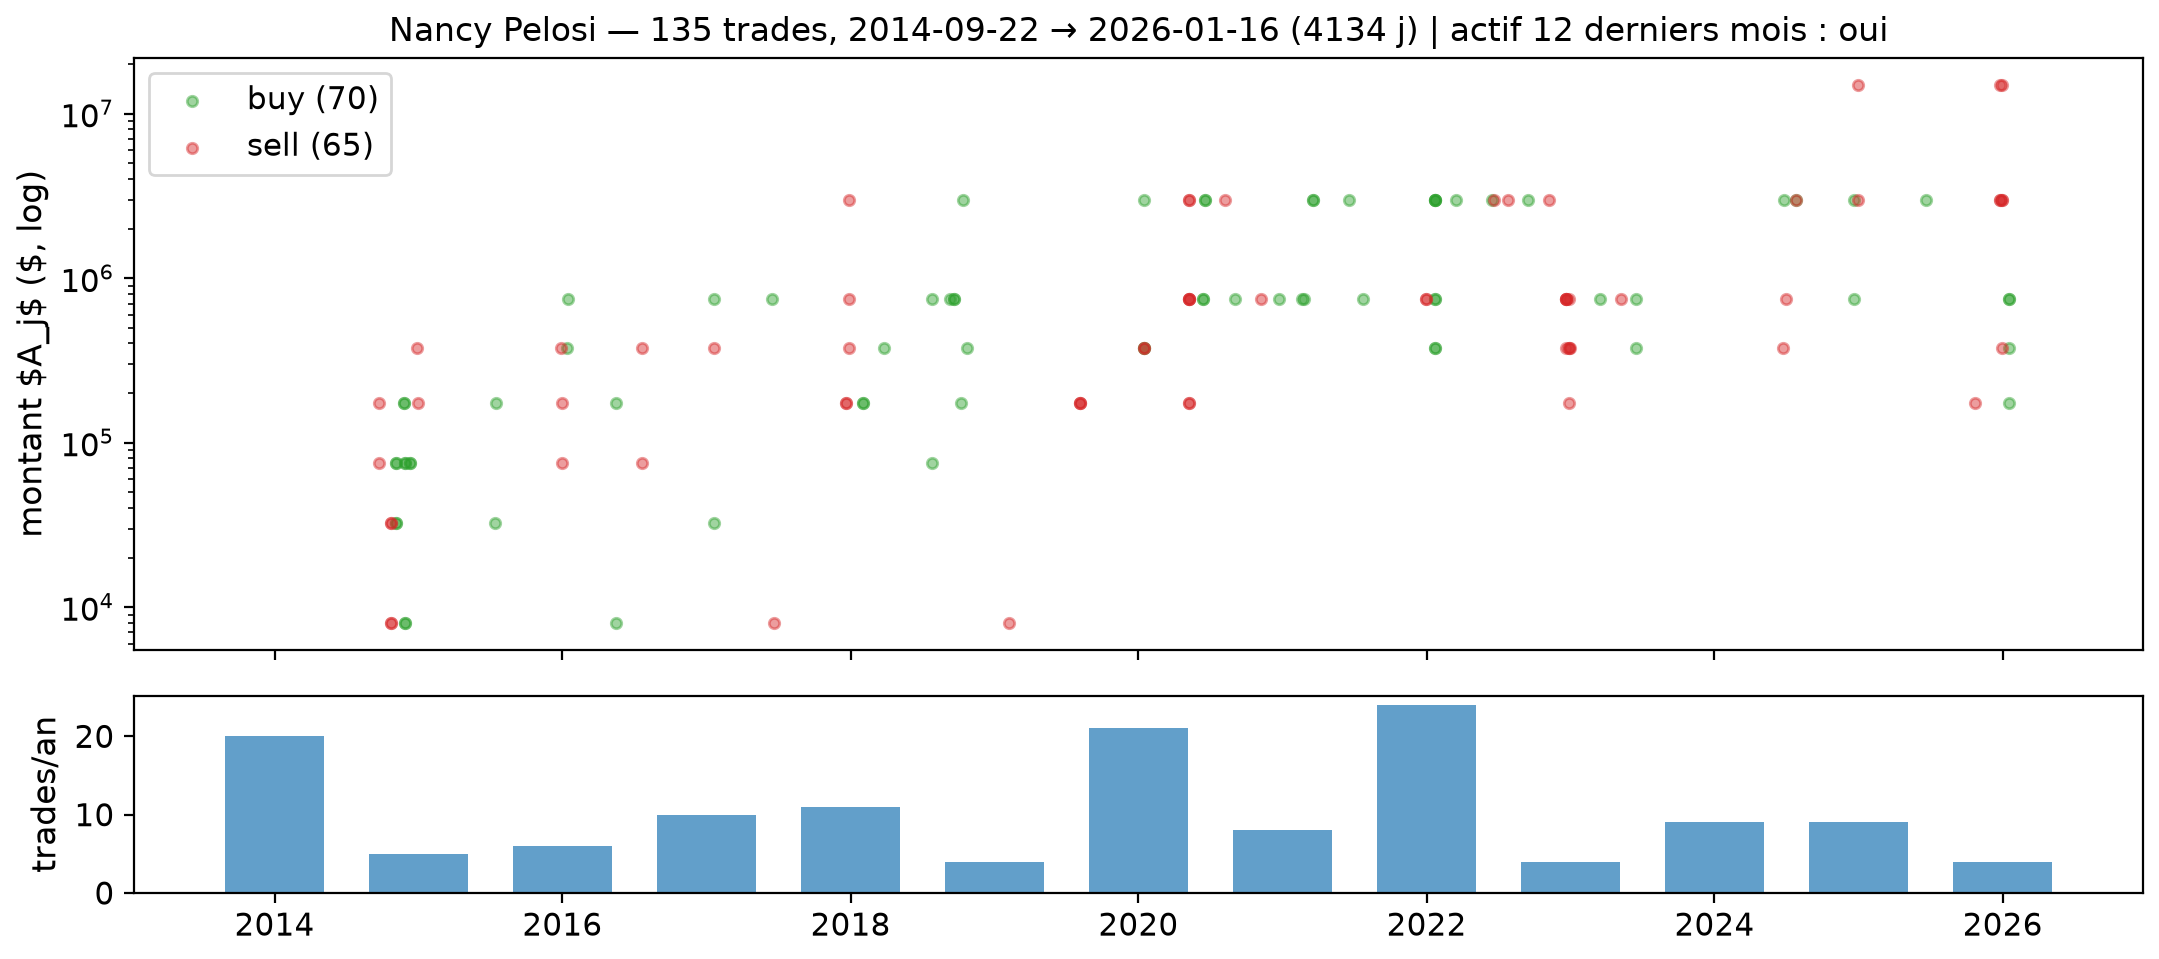
\includegraphics[height=0.52\textheight,width=0.9\textwidth,keepaspectratio]{png/figs_deck/fig_09_activite.png}\\[2mm]
  {\footnotesize chaque point est un trade daté et monté — \textcolor{okgreen}{\textbf{achats en vert}},
   \textcolor{alertred}{\textbf{ventes en rouge}}, montants $A_j$ en échelle log
   (leur somme : \co{notional\_total}) ; en bas, le rythme par année}
\end{frame}

% ── T5 · La fiche (3/6) : portefeuille ──
\begin{frame}{La fiche (3/6) — portefeuille : reconstruit jour après jour}
  \centering
  \bmaths{colonnes \co{hhi} (\co{n\_eff} $=1/$\co{hhi}) · \co{top1\_part} · \co{turnover}}%
    {\mathrm{hhi}=\mathrm{moy}_t\Bigl[\textstyle\sum_k w_k^m(t)^2\Bigr]\qquad
     \mathrm{turnover}=\frac{\sum_j A_j}{2\,\overline{V}_m}\cdot\frac{252}{T_m}}
  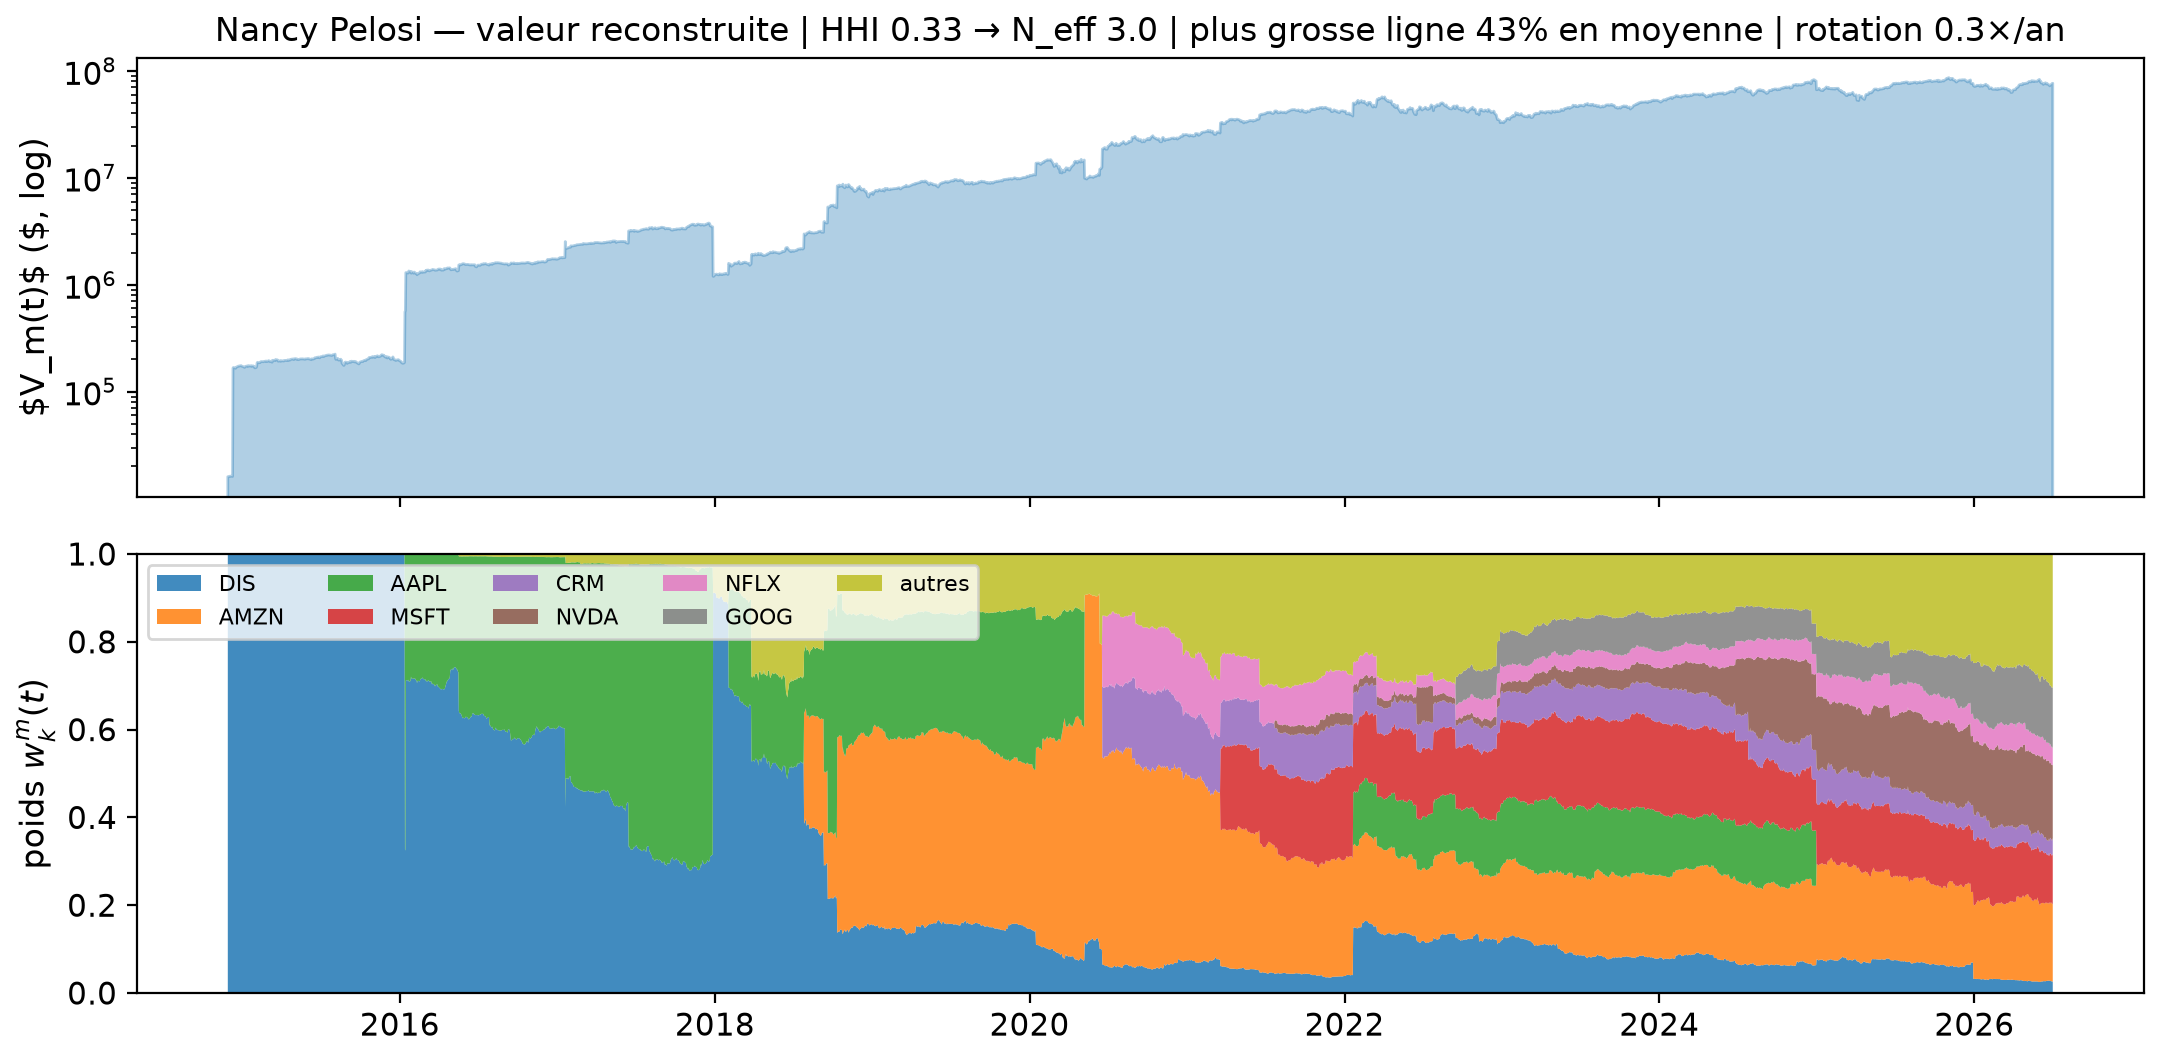
\includegraphics[height=0.46\textheight,width=0.9\textwidth,keepaspectratio]{png/figs_deck/fig_09_portefeuille.png}\\[2mm]
  {\footnotesize la reconstruction \textbf{FIFO datée} donne la valeur $V_m(t)$ et les poids de chaque
   titre à chaque instant — le rendement est \textbf{time-weighted}, jamais estimé}\\[1.5mm]
  \badge{helec}{un portefeuille en parts, valorisé jour par jour}
\end{frame}

% ── T6 · La fiche (4/6) : durées ──
\begin{frame}{La fiche (4/6) — durées : la moitié vit plus de 910 jours}
  \centering
  \bmaths{colonnes \co{duree\_km\_med} · \co{duree\_med\_fermee}}%
    {\hat S_m(t)=\widehat{\mathbb{P}}\bigl(\text{part encore détenue}>t\bigr)\qquad
     \mathrm{km\_med}=\inf\{t:\hat S_m(t)\le 0{,}5\}}
  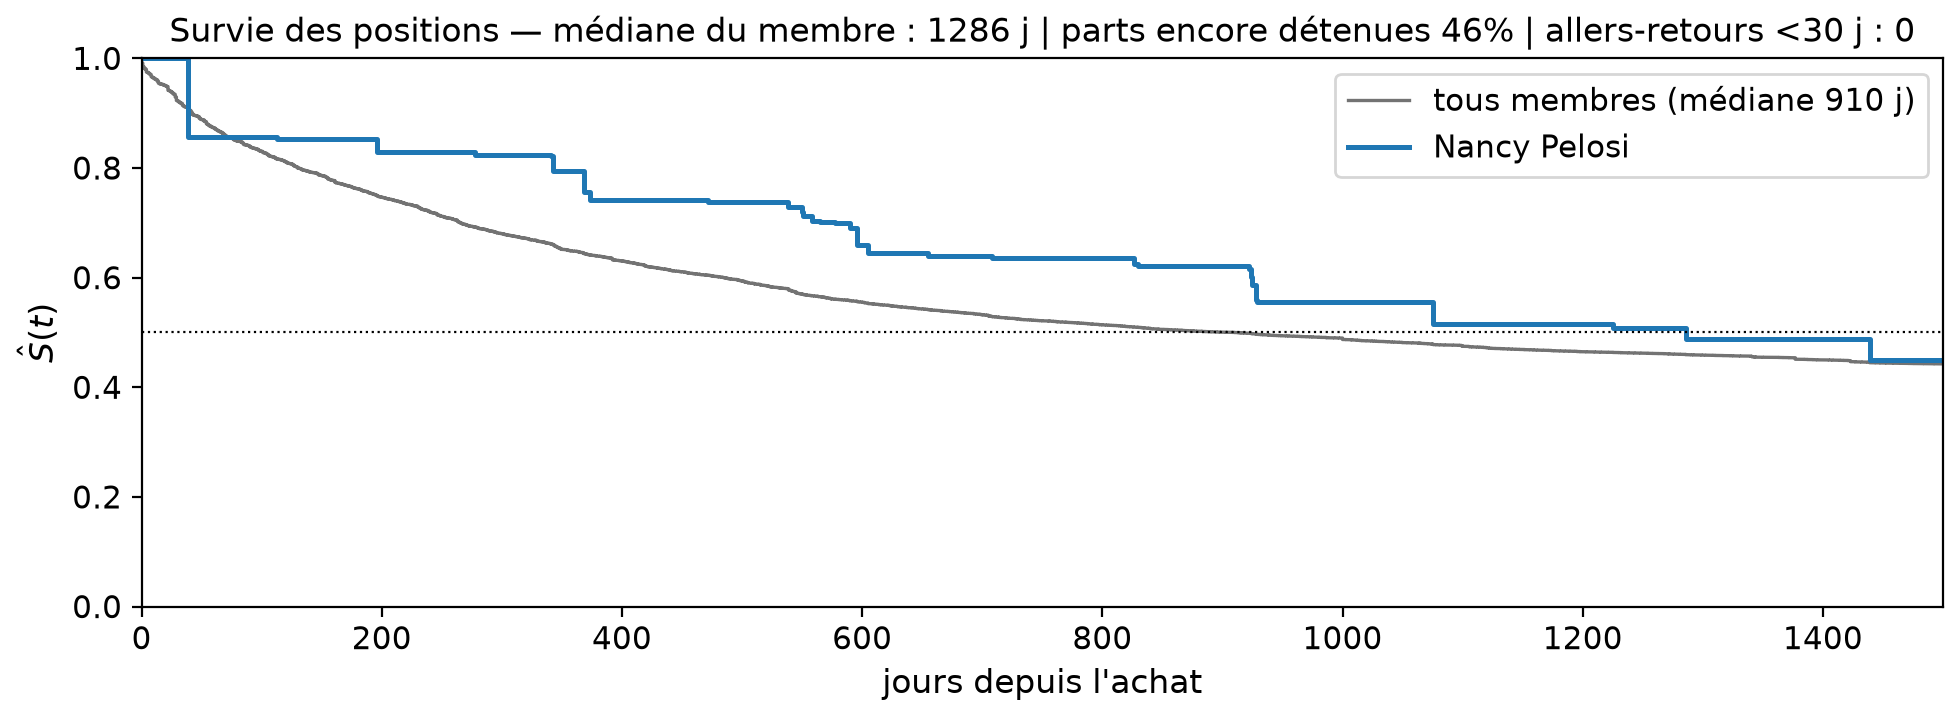
\includegraphics[width=0.72\textwidth,height=0.46\textheight,keepaspectratio]{png/figs_deck/fig_09_km.png}\\[2mm]
  {\footnotesize l'estimateur de \textbf{Kaplan-Meier} traite honnêtement les positions jamais
   revendues : \textbf{censurées}, pas ignorées — sinon les durées seraient sous-estimées}\\[1.5mm]
  \badge{warnorange}{44\,\% des parts jamais revendues (tous élus)}
\end{frame}

% ── T7 · La fiche (5/6) : risque et performance ──
\begin{frame}{La fiche (5/6) — risque \& perf : devant le SPY, sans certitude}
  \centering
  \bmaths{colonnes \co{sharpe} · \co{alpha\_ann} · \co{appraisal} — significatif si $|t|\ge 2$}%
    {\mathrm{sharpe}=\frac{\overline{r_m}}{\sigma(r_m)}\sqrt{252}\qquad
     r_m=\alpha+\beta\,r_{\mathrm{SPY}}+\varepsilon\ \Rightarrow\
     \mathrm{appraisal}=\frac{\alpha}{\sigma(\varepsilon)}\sqrt{252}}
  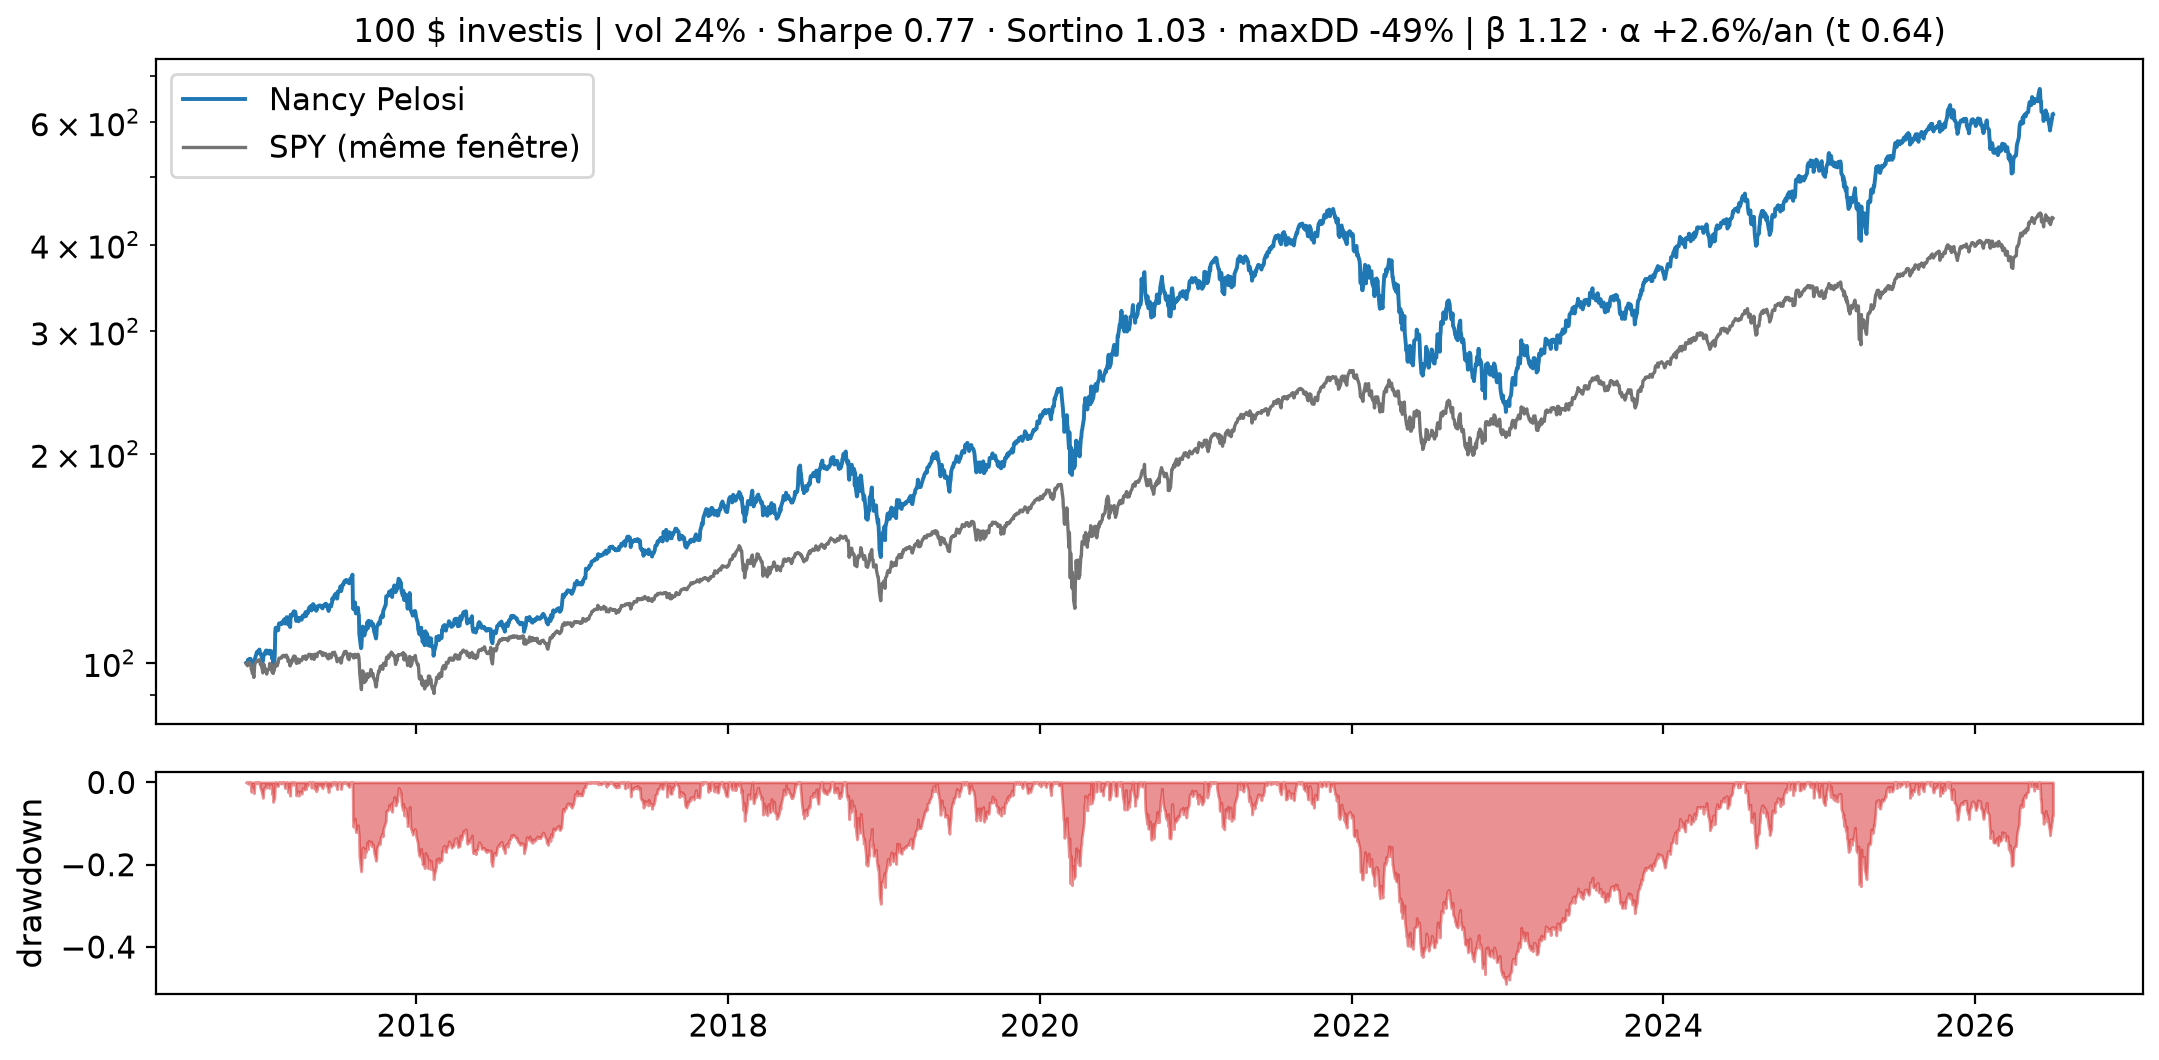
\includegraphics[height=0.40\textheight,width=0.9\textwidth,keepaspectratio]{png/figs_deck/fig_09_nav.png}\\[2mm]
  {\footnotesize +3,4\,\% de croissance par an au-dessus du SPY\ldots{} mais ni l'alpha
   ($t$ = 0,64) ni l'IR ($t$ = 1,06) ne passent le seuil de 2 : \textbf{indiscernable de la chance}}\\[1.5mm]
  \badge{okgreen}{+3,4\,\%/an vs SPY}\;
  \badge{warnorange}{aucun $t$ ≥ 2 — non significatif}
\end{frame}

% ── T9 · La fiche (6/6) : comportement ──
\begin{frame}{La fiche (6/6) — comportement : trois signaux, trois colonnes}
  \centering
  \bmaths{colonnes \co{part\_ci\_achats} · \co{part\_coachat} ($\ge 3$ acheteurs le même mois) ·
          \co{part\_trades\_repetes} (titre déjà tradé)}%
    {\mathrm{part\_ci}=\mathbb{P}\bigl(\mathrm{GICS}(k_j)\in J(\mathrm{comites}_m)\,\big|\,\mathrm{buy}\bigr)}
  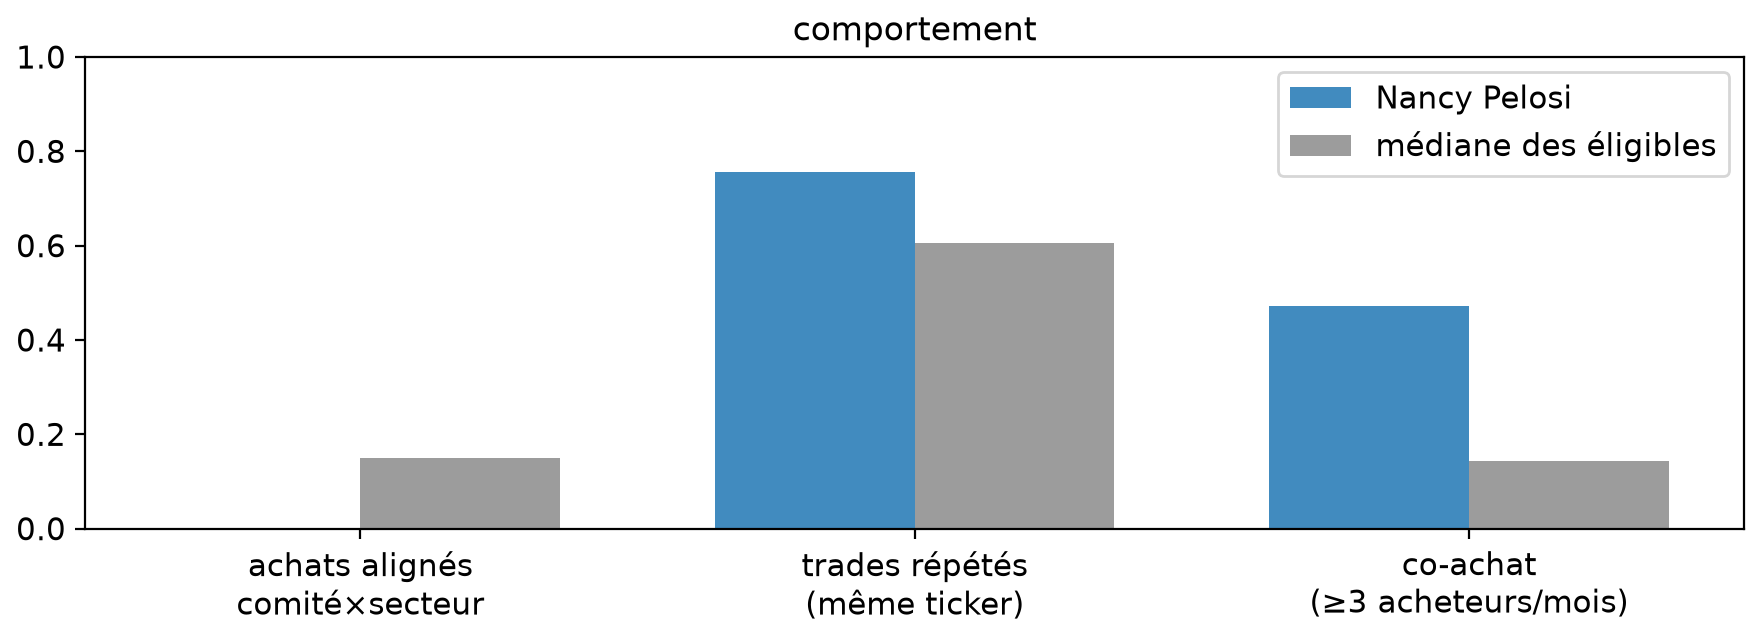
\includegraphics[width=0.64\textwidth,height=0.40\textheight,keepaspectratio]{png/figs_deck/fig_09_comportement.png}\\[2mm]
  {\footnotesize alignement avec ses comités ($J$ = les \co{secteurs\_juridiction} de la famille 1),
   répétition, co-achat : trois signaux mesurés pour chaque élu, comparés à la médiane des 223}\\[1.5mm]
  \badge{warnorange}{16,4\,\% des achats alignés comité (tous élus)}
\end{frame}

% ── T8 · Le pivot vers le panel ──
\begin{frame}{Le duel vs SPY, année par année : le panel annuel}
  \centering
  \bmaths{colonnes \co{ret\_annee} · \co{exces\_spy\_annee} (NaN si $<40$ j cotés dans l'année)}%
    {\mathrm{ret\_annee}=\prod_{t\in Y}\bigl(1+r_m(t)\bigr)-1\qquad
     \mathrm{exces\_spy\_annee}=\mathrm{ret\_annee}-\mathrm{ret\_annee}^{\mathrm{SPY}}\ \text{(mêmes jours)}}
  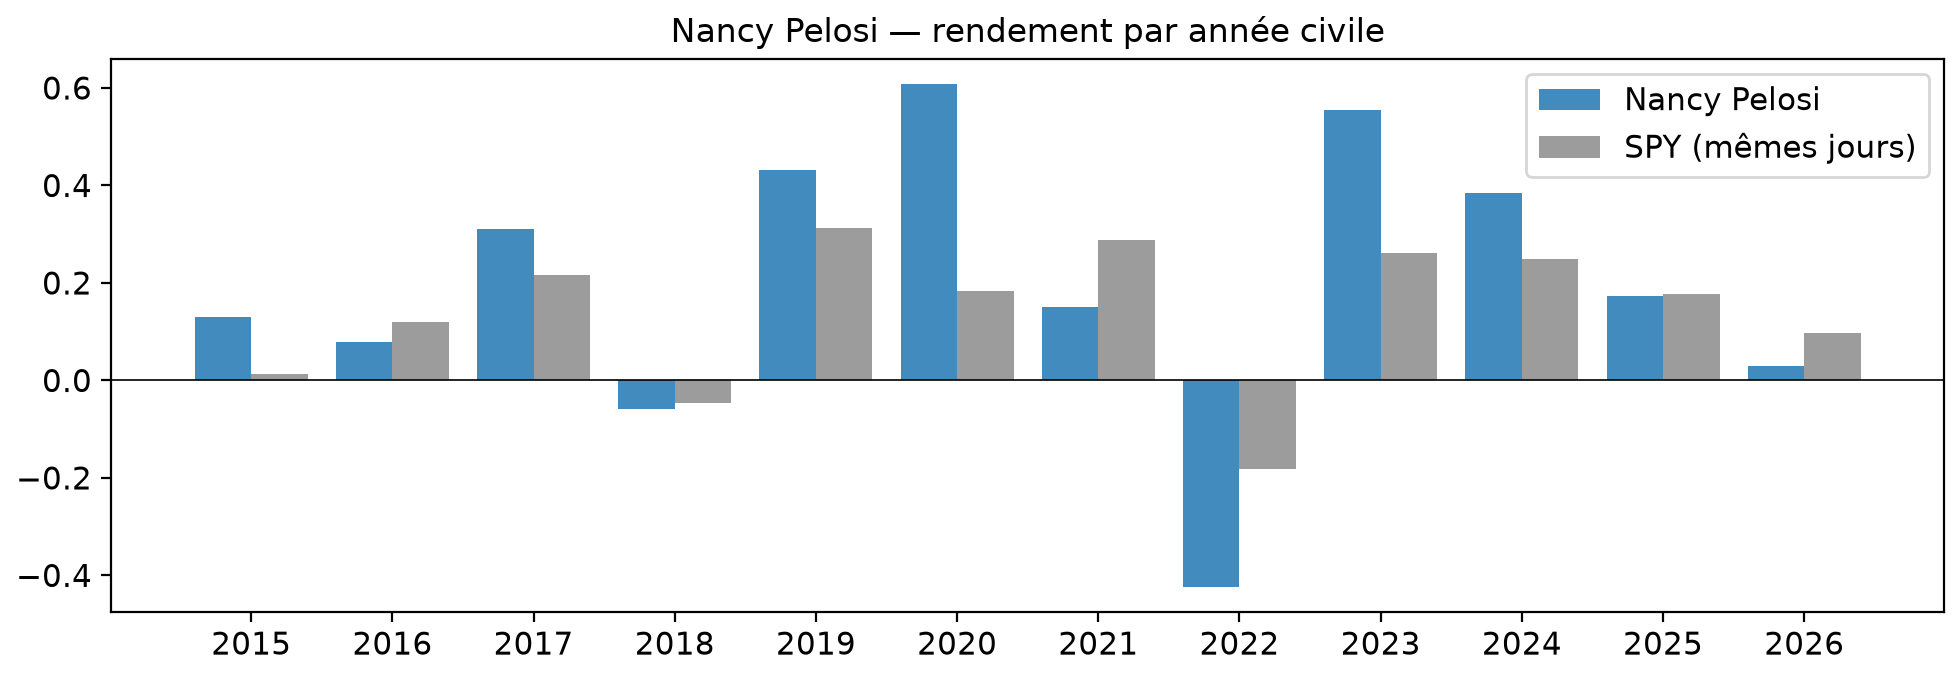
\includegraphics[width=0.76\textwidth,height=0.52\textheight,keepaspectratio]{png/figs_deck/fig_09_annees.png}\\[2mm]
  {\footnotesize chaque barre est une ligne de \co{membres\_annees.csv} —
   2\,628 couples (élu, année) prêts pour l'économétrie}\\[1.5mm]
  \badge{dataC}{2\,628 × 11}
\end{frame}

% ── T10 · Renversement : le ticker ──
\begin{frame}{Le même récit, vu du ticker : NVDA sous l'œil du Congrès}
  \centering
  \bmaths{colonnes \co{notional\_net} · \co{exces\_21j\_moy} / \co{exces\_63j\_moy}}%
    {\mathrm{notional\_net}=\!\!\sum_{d_j=\mathrm{buy}}\!\!A_j\ -\!\!\sum_{d_j=\mathrm{sell}}\!\!A_j\qquad
     \mathrm{exces}_H=\mathrm{moy}\Bigl[\tfrac{P_k(\tau+H)}{P_k(\tau)}-\tfrac{\mathrm{SPY}(\tau+H)}{\mathrm{SPY}(\tau)}\Bigr],\ H\in\{21,63\}\ \text{j}}
  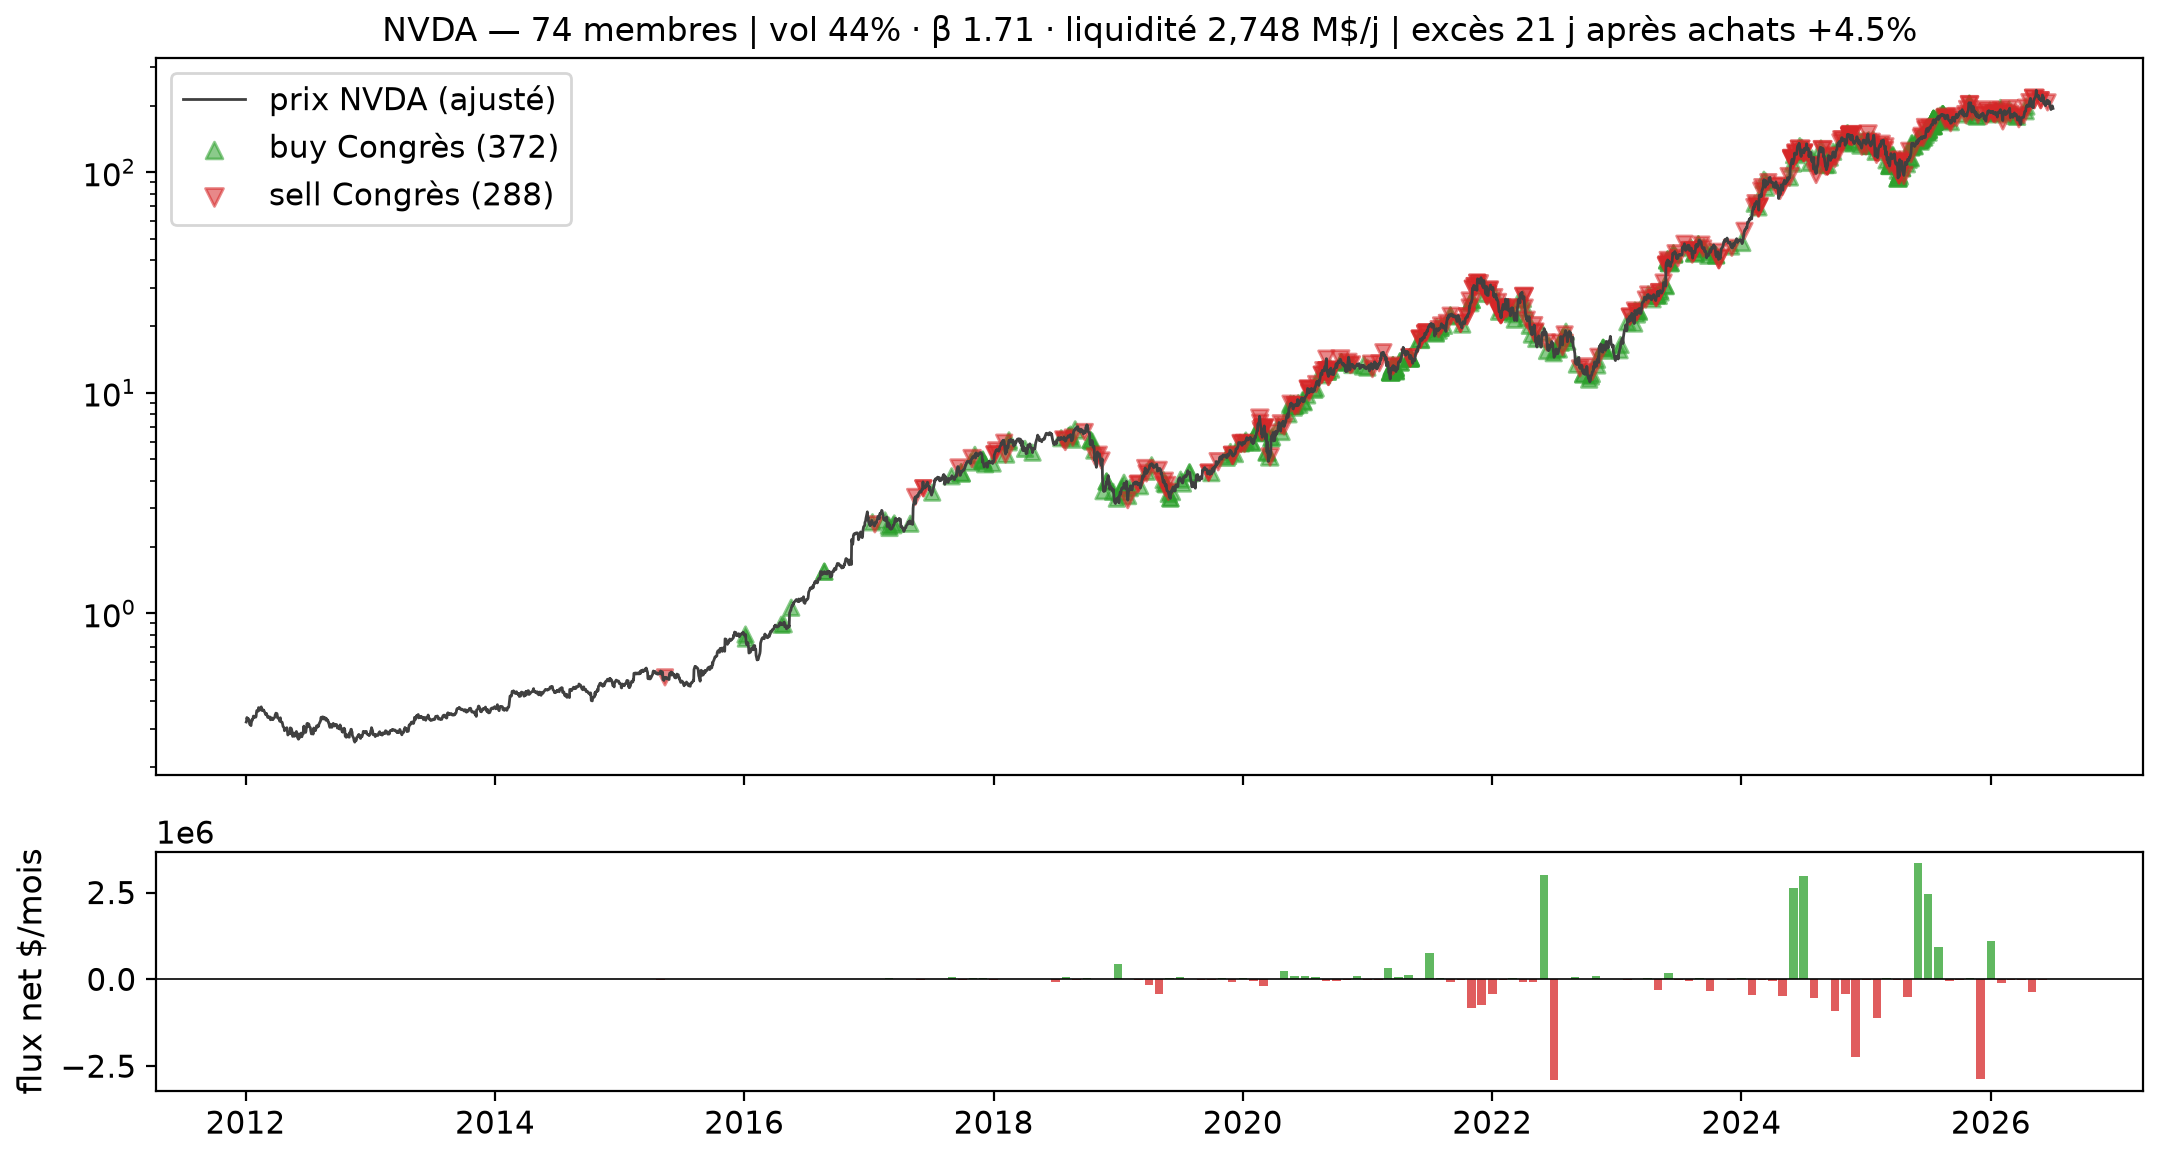
\includegraphics[height=0.44\textheight,width=0.9\textwidth,keepaspectratio]{png/figs_deck/fig_09_ticker_nvda.png}\\[2mm]
  {\footnotesize \co{tickers.csv} renverse la perspective : pour 4\,618 titres,
   \textbf{qui achète, qui vend, et quand} — triangles proportionnels aux montants}\\[1.5mm]
  \badge{dataC}{4\,618 × 40}
\end{frame}

% ── T11 · Renversement : la population ──
\begin{frame}{D'une élue aux 223 : les distributions derrière les fiches}
  \centering
  \bmaths{colonnes \co{vol\_ann} · \co{beta\_spy} (les autres : déjà définies, vues en distribution)}%
    {\mathrm{vol\_ann}=\sigma\bigl(\Delta\log P_k\bigr)\sqrt{252}\qquad
     \beta_{\mathrm{spy}}=\mathrm{cov}(r_k,r_{\mathrm{SPY}})/\mathrm{var}(r_{\mathrm{SPY}})}
  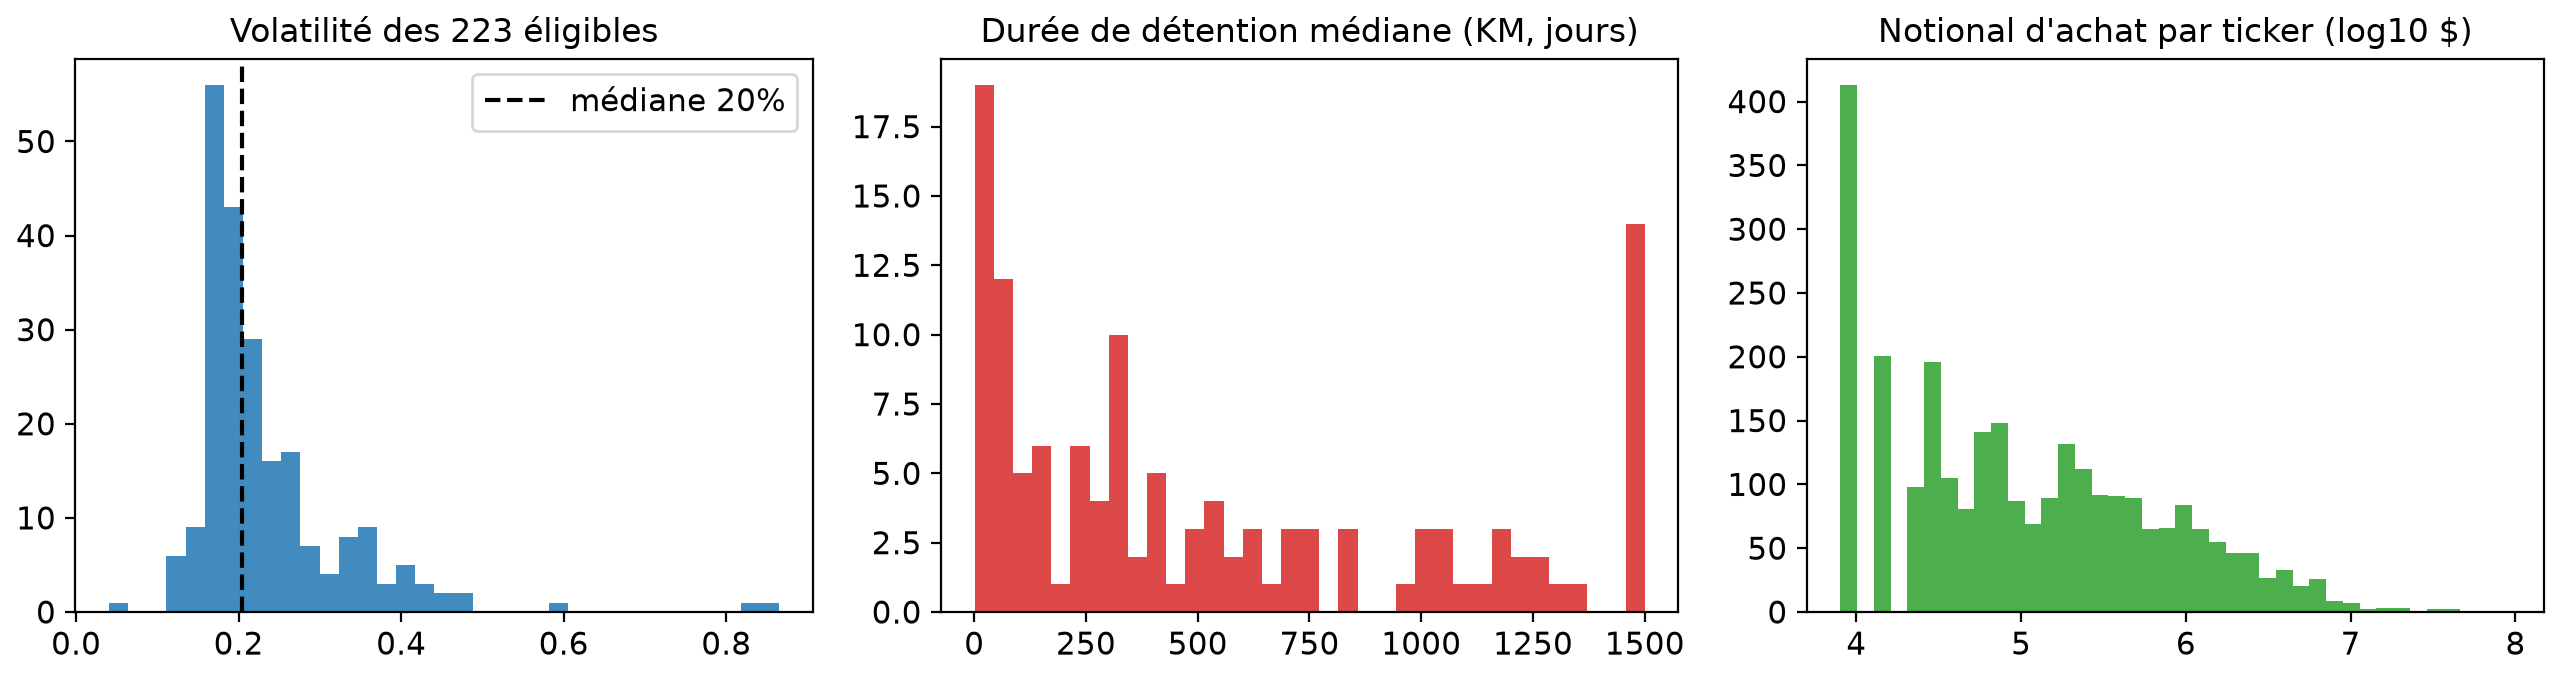
\includegraphics[width=0.84\textwidth,height=0.52\textheight,keepaspectratio]{png/figs_deck/fig_09_distributions.png}\\[2mm]
  {\footnotesize volatilité, durées de détention, notionnels par titre :
   chaque statistique individuelle se lit dans sa distribution}\\[1.5mm]
  \badge{helec}{223 élus éligibles}
\end{frame}

% ── T12 · Le verdict ──
\begin{frame}{Le verdict, trade par trade — 58\,926 achats notés face au SPY}
  \centering
  {\scriptsize\color{black!55} colonnes \co{exces\_med\_trade} · \co{hit\_rate} —
   chaque achat est noté contre le SPY, sur \textbf{sa} fenêtre, \textbf{brut de frais}}\\[0.6mm]
  {\color{helec}\scriptsize\textbf{1 · la sortie} — premier des deux : revente réelle, ou plafond d'un an}\\[0.2mm]
  {\small $t^{s}_j=\min\bigl(\text{1\iere{} vente de }(m_j,k_j)\ \text{après }\tau_j,\ \ \tau_j+252\ \text{j}\bigr)$}\\[0.6mm]
  {\color{dataC}\scriptsize\textbf{2 · la note} — l'excès sur le SPY entre l'achat et la sortie}\\[0.2mm]
  {\small $x_j=\Bigl[\tfrac{P_k(t^{s}_j)}{P_k(\tau_j^{+})}-1\Bigr]
          -\Bigl[\tfrac{\mathrm{SPY}(t^{s}_j)}{\mathrm{SPY}(\tau_j^{+})}-1\Bigr]
          \qquad \mathrm{hit\_rate}=\mathbb{P}(x_j>0)$}\\[2mm]
  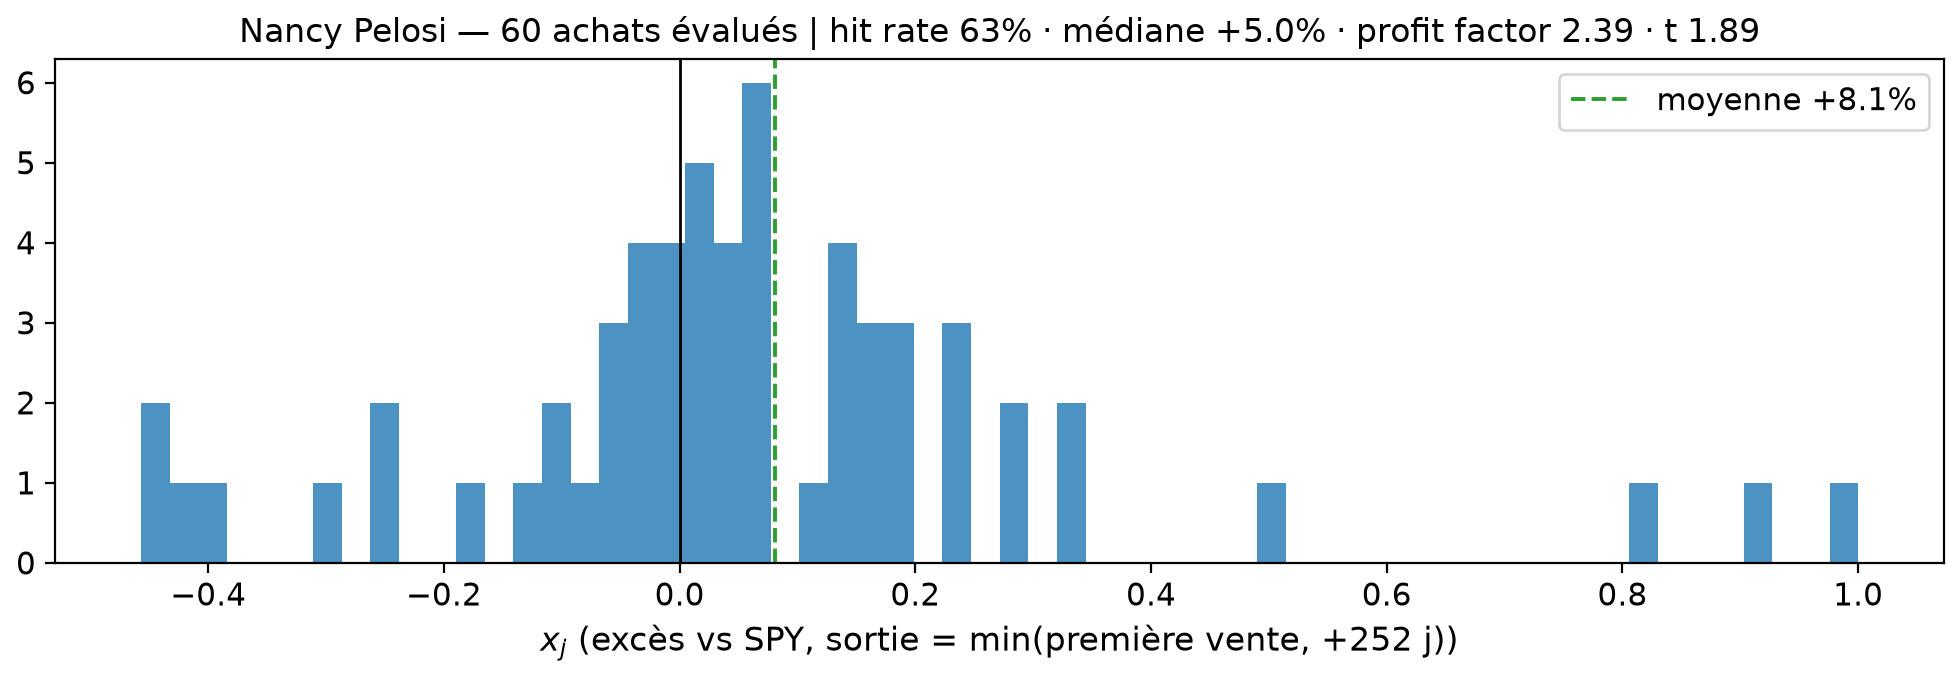
\includegraphics[width=0.60\textwidth,height=0.30\textheight,keepaspectratio]{png/figs_deck/fig_09_exces.png}\\[1.5mm]
  {\footnotesize même pour elle — 63\,\% d'achats gagnants, médiane +5,0\,\% — le $t$ reste
   \textbf{sous 2} ; l'élu médian, lui, sous-performe : \textbf{−1,62\,\%} (58\,926 achats)}\\[1.5mm]
  \badge{warnorange}{elle : $t$ = 1,89 $<$ 2}\;
  \badge{alertred}{tous élus : excès médian −1,62\,\%}
\end{frame}

% ── T13 · Clôture : les garanties ──
\begin{frame}{8 contrôles sur 8 — la valeur de ces tables, c'est leur transparence}
  \centering
  \vspace{1mm}
  \tuile{okgreen}{8\,/\,8}{contrôles croisés\\entre les 3 tables}\hfill
  \tuile{dataC}{4 CSV}{livrés, chaque colonne\\documentée}\hfill
  \tuile{helec}{3 preuves}{recalcul à la main ·\\2\ieme{} méthode · recoupements}\hfill
  \tuile{alertred}{0 alpha}{significatif dans\\les fiches}\\[5mm]
  \fcolorbox{dataC}{white}{\parbox{0.80\textwidth}{\centering\footnotesize
    les 8 contrôles sont des \co{assert} \textbf{bloquants}, exécutés \textbf{avant} l'écriture
    (\S13 puis \S14 du notebook) — les 4 CSV livrés dans \co{tables/} sont, par construction,
    ceux d'une exécution où les \textbf{8/8} sont passés}}\\[4mm]
  {\footnotesize nous ne livrons pas un alpha, nous livrons des \textbf{données comprises} —
   la stratégie peut maintenant commencer}
  \label{endmain}% dernière page de contenu (les zooms ne comptent pas)
\end{frame}




% ══════════════════ FRAMES DE ZOOM (agrandissement des captures, hors comptage) ══════════════════
\zoomframe{scan_full_droit}{png/figs_deck/scan_full_droit.png}
\zoomframe{scan_full_manuscrit}{png/figs_deck/scan_full_manuscrit.png}
\zoomframe{site_house_clerk}{png/figs_deck/site_house_clerk.png}
\zoomframe{fichier_index_xml}{png/figs_deck/fichier_index_xml.png}
\zoomframe{house_digital}{png/figs_deck/house_digital.png}
\zoomframe{house_ocr}{png/figs_deck/house_ocr.png}
\zoomframe{site_senate_form}{png/figs_deck/site_senate_form.png}
\zoomframe{senate_digital_1}{png/figs_deck/senate_digital.png}
\zoomframe{senat_papier_droit_1}{png/figs_deck/senat_papier_droit.png}
\zoomframe{fig_ptr_multiligne}{png/figs_deck/fig_ptr_multiligne.png}
\zoomframe{senate_digital_2}{png/figs_deck/senate_digital.png}
\zoomframe{senat_papier_droit_2}{png/figs_deck/senat_papier_droit.png}
\zoomframe{sp_tape}{png/figs_deck/senat_papier_droit.png}
\zoomframe{sp_manu}{png/figs_deck/senat_papier_manuscrit.png}
\zoomframe{sp_annexe}{png/figs_deck/senat_papier_annexe_v.png}
\zoomframe{fig_pelosi_schedb}{png/figs_deck/fig_pelosi_schedb.png}
\zoomframe{fig_ptr_digital}{png/figs_deck/fig_ptr_digital.png}
\zoomframe{site_senate_results}{png/figs_deck/site_senate_results.png}
\zoomframe{ftype_x}{png/figs_deck/ftype_x.png}
\zoomframe{ftype_d}{png/figs_deck/ftype_d.png}
\zoomframe{ftype_w}{png/figs_deck/ftype_w.png}
\zoomframe{ftype_e}{png/figs_deck/ftype_e.png}
\zoomframe{ftype_g}{png/figs_deck/ftype_g.png}
\zoomframe{ftype_b}{png/figs_deck/ftype_b.png}

\end{document}
